\documentclass[10.5pt, A4paper, openany, uplatex]{book}
\usepackage[dvipdfmx]{graphicx}
\usepackage[dvipdfmx]{color}
\usepackage[dvipdfmx, colorlinks = true, linkcolor = blue, filecolor = blue, urlcolor = blue, citecolor = blue]{hyperref}
\usepackage{amsfonts}
\usepackage{amssymb}
\usepackage{amsmath}
\usepackage{ascmac}
\usepackage{framed}
\usepackage{comment}
\usepackage{latexsym}
\usepackage{endnotes}
\usepackage{mathrsfs}
\usepackage{longtable}
\usepackage[left=2.2cm,top=2cm,right=2.2cm,bottom=2cm]{geometry}
\usepackage{theorem}
\usepackage{lscape}
\usepackage{bm}
\usepackage{url}
\usepackage{listings}
\usepackage{makeidx}
\usepackage[titletoc]{appendix}
\usepackage{fdsymbol}

\DeclareMathOperator*{\plim}{plim}

\newcommand{\mbf}{\mathbf}
\newcommand{\mcl}{\mathcal}
\newcommand{\mbb}{\mathbb}
\newcommand{\mrm}{\mathrm}
\newcommand{\msc}{\mathscr}
\newcommand{\tr}{\top}
\newcommand{\eps}{\varepsilon}
\newcommand{\R}{\textbf{R}}
\newcommand{\E}{\mathbb{E}}
\newcommand{\Var}{\mathrm{Var}}
\newcommand{\Cov}{\mathrm{Cov}}

\renewcommand{\hat}{\widehat}
\renewcommand{\tilde}{\widetilde}
\renewcommand{\bar}{\overline}

\newtheorem{theorem}{Theorem}[section]
\newtheorem{acknowledgement}[theorem]{Acknowledgement}
\newtheorem{algorithm}[theorem]{Algorithm}
\newtheorem{axiom}[theorem]{Axiom}
\newtheorem{case}[theorem]{Case}
\newtheorem{claim}[theorem]{Claim}
\newtheorem{conclusion}[theorem]{Conclusion}
\newtheorem{condition}[theorem]{Condition}
\newtheorem{conjecture}[theorem]{Conjecture}
\newtheorem{corollary}[theorem]{Corollary}
\newtheorem{criterion}[theorem]{Criterion}
\newtheorem{definition}[theorem]{Definition}
\newtheorem{example}[theorem]{Example}
\newtheorem{exercise}[theorem]{Exercise}
\newtheorem{lemma}[theorem]{Lemma}
\newtheorem{notation}[theorem]{Notation}
\newtheorem{problem}[theorem]{Problem}
\newtheorem{proposition}[theorem]{Proposition}
{\theorembodyfont{\upshape}
\newtheorem{remark}{Remark}
}
\newtheorem{solution}[theorem]{Solution}
\newtheorem{summary}[theorem]{Summary}
\newenvironment{proof}[1][Proof]{\textbf{#1.} }{\  \rule{0.5em}{0.5em}}
\newtheorem{assumption}{Assumption}
\oddsidemargin=0cm \evensidemargin=0cm
\numberwithin{equation}{section}
\def \baselinestretch{1.4}

\newcommand{\indep}{\mathrel{\text{\scalebox{1.07}{$\perp\mkern-10mu\perp$}}}}
\DeclareMathOperator*{\argmin}{\arg\!\min}
\DeclareMathOperator*{\argmax}{\arg\!\max}
\DeclareMathOperator*{\argsup}{\arg\!\sup}
\DeclareMathOperator*{\arginf}{\arg\!\inf}

\allowdisplaybreaks

\graphicspath{{./figs/}}
\bibliographystyle{apalike} 

\title{
	\textbf{Advanced Econometrics}\footnote{Updated irregularly. Please check the course page occasionally for the latest version.} \\
	\Large \flushleft{Part I.\hspace{5pt}  Methods of Econometrics} \\
	\Large \flushleft{Part II. Econometric Analysis of Cross-Sectional Dependence Models}	
}

\normalsize

\author{Tadao Hoshino (���싧�Y)\thanks{
		School of Political Science and Economics, Waseda University. 1-6-1 Nishi-waseda, Shinjuku-ku, Tokyo 169-8050, Japan. Email: thoshino@waseda.jp. 
		If you find any typos and errors please let me know.}}
\date{\today}
\makeindex

\begin{document}
\frontmatter
\maketitle
\tableofcontents
\mainmatter 

%%%%%%%%%%%%%%%%%%%%%%%%%%%%%%%%%%%%%%%%%%%%%%%%
\part{Methods of Econometrics}
%%%%%%%%%%%%%%%%%%%%%%%%%%%%%%%%%%%%%%%%%%%%%%%%

\chapter{Consistency and Asymptotic Normality}\label{chap:LLN_CLT}
\section{Convergence of real sequences}
Real numbers are numbers that have points on the number line $\mathbb{R}$.
Let $a$ be a real number and $(a_n)_{n=1}^\infty$ be a sequence of real numbers:
\[
	(a_n)_{n=1}^\infty = a_1, \; a_2, \; a_3, \ldots
\]
For example, a sequence
\[
	a_1 = 1, \; a_2 = 1.4, \; a_3 = 1.41, \; \cdots, \; a_n = 1.4142\ldots, \cdots
\]
gets closer and closer to $\alpha = \sqrt{2} \; (= 1.414213\ldots)$ as $n$ increases.
The number $\alpha$ is called the \textbf{limit\index{limit}} of the sequence $(a_n)_{n=1}^\infty$. 
We say that the sequence $(a_n)_{n=1}^\infty$ \textbf{converges\index{convergence}} to $\alpha$, and write
\begin{align*}
	& \lim_{n\to\infty}a_n = \alpha \\
	\text{or equivalently} \;\; & a_n \to \alpha \;\; (n\to\infty).
\end{align*}

For other examples, the limit of the sequence $a_1 = 1, \; a_2 = 1/2, \; a_3 = 1/3, \; \cdots, \; a_n = 1/n, \cdots$ is clearly $\lim_{n\to\infty}a_n = 0$.
It is well-known that the sequence
\[
	a_1 = (1 + (1/1))^1, \; a_2 = (1 + (1/2))^2, \; \cdots, \; a_n = (1 + (1/n))^n, \cdots
\]
converges to the Napier's constant: $\lim_{n\to\infty}a_n = e \; (=2.718 \cdots)$.
On the other hand, the limit of the sequence $a_1 = 1, \; a_2 = 2, \; a_3 = 3, \;\cdots, \; a_n = n, \cdots$ is infinite: $\lim_{n\to\infty}a_n = \infty$.
When the limit of a sequence is infinite, we say that the sequence is a \textbf{divergent\index{divergent}}.
There are sequences that are neither convergent nor divergent.
For example, the sequence
\[
	a_1 = -1, \; a_2 = 1, \; a_3 = -1, \; \cdots, \; a_n = (-1)^n, \cdots
\]
alternates between $1$ and $-1$.

The statement ``the sequence $(a_n)_{n=1}^\infty$ gets closer to $\alpha$ as $n$ increases'' is rather informal and mathematically unclear.
A formal definition of convergence is as follows.

\begin{definition}\label{def:conv}
We say that a sequence of real numbers $(a_n)_{n=1}^\infty$ converges to a limit $\alpha$ if for any given positive number $\kappa > 0$, there exists a natural number $n(\kappa)$ such that
\begin{equation}
	|a_n - \alpha| < \kappa \;\; \text{for all $n$ satisfying } n(\kappa) \leq n. \label{eq:conv}
\end{equation}
\end{definition}

The interpretation of \eqref{eq:conv} is as follows.
Choose an arbitrary small $\kappa$, say $\kappa < 10^{-100}$ or even smaller.
Even for such a small value of $\kappa$, if we set $n(\kappa)$ sufficiently large, the distance between the terms of the sequence after $a_{n(\kappa)}$ and $\alpha$ can be smaller than $\kappa$ (see Figure \ref{fig:limit}).
 
\begin{figure}[h!]
	\begin{center}
	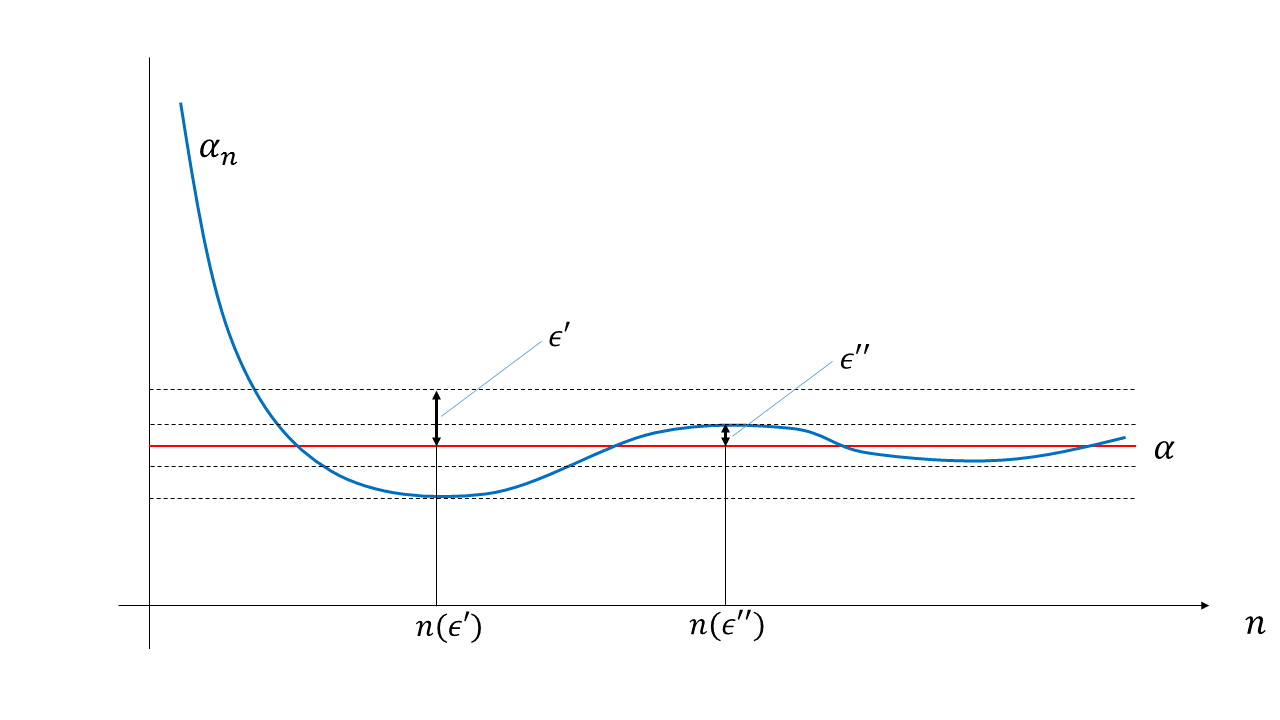
\includegraphics[width=14cm]{Limit.png}\label{fig:limit}
	\caption{Convergence of a real sequence}
	\end{center}
\end{figure}

\begin{framed}
\begin{exercise}\label{ex:seq}\upshape
	What are the limits of the following sequences?
	\begin{enumerate}
		\item $a_n = n^2 - n$
		\item $a_n = (-1)^n/\sqrt{n}$
		\item $a_n = \sqrt{n + 1} - \sqrt{n}$
	\end{enumerate}
\end{exercise}
\begin{exercise}\upshape
	Prove that the infinite decimal $0.999 \ldots$ is equal to one using the notion of convergence and limit.
\end{exercise}
\begin{exercise}\upshape
	Let $S_n = \sum_{k=1}^n a_k$ and $\bar S_n = \sum_{k=1}^n |a_k|$.
	Show that if $\bar S_n$ converges to a finite number, so does $S_n$. (This is called \textbf{absolute convergence}.)
\end{exercise}
\end{framed}

Note  that $a_k \to 0$ as $k \to \infty$ does not ensure the convergence of $S_n = \sum_{k = 1}^n a_k$ at all.
For example, as is well known, $\sum_{k = 1}^n k^{-1}$ diverges to infinity.\footnote{
	Proof: Observe that
	\begin{align*}
		\exp(1 + 2^{-1} + 3^{-1} + \cdots + n^{-1})
		& = \exp(1)\exp(2^{-1})\exp(3^{-1})\cdots\exp(n^{-1}) \ge (1 + 1)(1 + 2^{-1})(1 + 3^{-1})\cdots(1 + n^{-1}) \\
		& = 2 \cdot \frac{3}{2} \cdot \frac{4}{3} \cdots \frac{n + 1}{n} = n + 1,
	\end{align*}
	where we have used the fact $\exp(x) \ge 1 + x$.
	This implies that $1 + 2^{-1} + 3^{-1} + \cdots + n^{-1} \ge \log (n + 1)$, where the right-hand side diverges as $n$ tends to infinity.
}

\section{Convergence in probability}\label{subsec:inprob}

Now let $Z_n \in \mbb{R}$ be a  sequence of ``random variables''.
Recall that random variables are not numbers, but they are functions (rules) that assign some real numbers to random events.
Thus, whether the sequence of random variables $Z_n$ converges to a limit or not is itself a stochastic event, and hence the definition \ref{def:conv} cannot be applied directly.
However, since a probability is a real number, we can still consider the convergence of a sequence of probabilities in the usual sense.
Then, we introduce the notion of ``convergence in probability''.

\begin{definition}
For any given positive number $\kappa > 0$, if
\[
	\lim_{n \to \infty} \Pr(|Z_n - \mu| \le \kappa) = 1
\]
holds, we say that $Z_n$ \textbf{converges in probability\index{convergence in probability}} to $\mu$ as $n \to \infty$, and write 
\begin{align*}
	& \plim_{n \to \infty} Z_n = \mu \\
	\text{or equivalently} \;\; &  Z_n \overset{p}{\to} \mu \;\; (n\to\infty).
\end{align*}
\end{definition}

The above definition can be read as follows: $a_n \equiv \Pr(|Z_n - \mu| \le \kappa)$, which is a real number, converges to one for any $\kappa$ in the sense of Definition \ref{def:conv}.
It is important to note that $\mu$ can be either a random variable or a constant number in this definition.

When $Z_n$ is a sequence of vector-valued random variables, one can use an appropriate norm $||\cdot||$, such as the Euclidean norm, in place of the absolute value $|\cdot|$.\footnote{
	Throughout, when not explicitly mentioned, $||\cdot||$ stands for the Euclidean norm (i.e., the square root of the sum of squared elements).
}
Note that the choice of $\kappa$ is arbitrary, and thus it can be, for example, $\kappa < 10^{-100}$ or even smaller as long as it is larger than 0.
This definition says that the probability of observing the event $\{|Z_n - \mu| \le \kappa\}$ approaches to one as $n$ increases even for such very small $\kappa$. 

Note that a constant is a special case of a random variable.
Therefore, when a sequence of constants converges $a_n \to \alpha$, it trivially holds that $a_n \overset{p}{\to} \alpha$.
Further, for a sequence of random variables that converges in probability $Z_n \overset{p}{\to} \mu$, we also have $a_n Z_n  \overset{p}{\to} \alpha \mu $ because
\begin{align*}
	|a_n Z_n - \alpha \mu| 
	& \le |a_n Z_n - a_n \mu| + |a_n \mu - \alpha \mu|\\
	& = |a_n| \cdot |Z_n - \mu| + |\mu| \cdot |a_n - \alpha| \overset{p}{\to} 0,
\end{align*}
where the inequality follows from the triangle inequality.

\begin{lemma}[Markov's inequality\index{Markov's inequality}]\label{markov}
	For any random variable $Z_n$ and positive constant $\kappa > 0$,
	\begin{equation}\label{eq:markov}
	\Pr\left( |Z_n| > \kappa \right) \leq \frac{\E|Z_n|}{\kappa}.
	\end{equation}
\end{lemma}

\begin{proof}
	First, observe the following equality:
	\begin{align*}
	\Pr( |Z_n| > \kappa ) 
	& = \E[\mbf{1}(|Z_n| > \kappa )] \\
	& = \E\left[\mbf{1}\left(\frac{|Z_n|}{\kappa} > 1 \right)\right]
	\end{align*}
	Since $\frac{|Z_n|}{\kappa}$ is non-negative, we have $\mbf{1}\left(\frac{|Z_n|}{\kappa} > 1 \right) \le \frac{|Z_n|}{\kappa}$.
	Hence,
	\begin{align*}
	\E\left[\mbf{1}\left(\frac{|Z_n|}{\kappa} > 1 \right)\right] \le \frac{\E|Z_n|}{\kappa}.
	\end{align*}
	This implies the desired result.
\end{proof}

As a corollary of Markov's inequality, we can obtain the following useful inequality:
\begin{align}\label{eq:chevyshev}
\Pr( |Z_n - \E Z_n | > \kappa ) = \Pr( (Z_n - \E Z_n)^2 > \kappa^2 ) \leq \frac{\Var(Z_n)}{\kappa^2},
\end{align}
which is known as \textbf{Chebyshev's inequality\index{Chevyshev's inequality}}.
Note that these inequalities do not make any assumptions about the probability distribution of $Z_n$; that is, they are distribution-free inequalities.
When $\E |Z_n|$ and $\Var(Z_n)$ do not exist, such that $\E |Z_n| = \infty$ and $\Var(Z_n) = \infty$, the inequalities  \eqref{eq:markov} and \eqref{eq:chevyshev} hold trivially.
\bigskip

Here, let $X \in \mbb{R}$ be a random variable, and $\bar X_n$ be the sample mean of $X$, where $n$ denotes the sample size.
Chebyshev's inequality implies that, if $\Var(\bar X_n) \to 0$ as $n \to \infty$,
\[
\Pr( |\bar X_n - \E \bar X_n | > \kappa ) \leq \frac{\Var(\bar X_n)}{\kappa^2} \to 0.
\]
In other words, since 
\[
	\Pr( |\bar X_n - \E\bar X_n | \le \kappa ) = 1 - \underbrace{\Pr( |\bar X_n - \E\bar X_n | > \kappa )}_{\to \: 0},
\]
the sample mean converges to its population mean in probability:
\[
\bar X_n \overset{p}{\to} \E\bar X_n.
\]
This result is known as the \textbf{weak law of large numbers\index{weak law of large numbers}} (WLLN).\footnote{	
	Since there is a ``weak'' LLN, there is also a ``strong'' version of LLN (SLLN), which states that $\Pr(\lim_{n \to \infty} \bar X_n = \E \bar X_n) = 1$.
	The proof of SLLN is much more complicated than that of WLLN.
	SLLN implies WLLN.}
As shown above, an easy-to-check sufficient condition for WLLN to hold is that $\Var(\bar X_n)$ converges to zero as $n$ increases.
In the case when the data $\{X_1, \ldots , X_n\}$ are independent and identically distributed (IID), the condition can be easily confirmed by the fact that $\Var(\bar X_n) = \Var(X)/n \to 0$ as $n \to \infty$ as long as $\Var(X)$ is finite.\footnote{
	That said, perhaps somewhat surprisingly, $\Var(X) < \infty$ is not a necessary condition for WLLN in general.
	}
\bigskip

An estimator which converges in probability to its population value is called a \textbf{consistent estimator\index{consistent estimator}}.
That is, letting $\hat\theta_n$ be an estimator of $\theta_0$ obtained from a sample of size $n$, if $\hat\theta_n \overset{p}{\to} \theta_0$, we say that $\hat\theta_n$ is consistent for $\theta_0$.
WLLN states that the sample mean is a consistent estimator of the population mean under IID sampling.

\begin{framed}
\begin{exercise}\upshape
	Suppose that $\{X_1, \ldots, X_n\}$ are independent, and
	\[
	X_n = \left\{\begin{array}{ll}
	0 & \text{ with probability } 1-1/n\\
	n & \text{ with probability } 1/n.
	\end{array}\right.
	\]
	Prove that $X_n$ converges to zero in probability.
\end{exercise}
\begin{exercise}\upshape
	Suppose that we have $n$ IID observations $\{X_1, \ldots, X_n\}$ drawn from $\text{Uniform}[0,1]$.
	Define 
	\[
	a_n \equiv \max\{X_1, \ldots, X_n\}.
	\]
	Prove that $a_n$ converges to one in probability.
\end{exercise}
\begin{exercise}\upshape
	(\textbf{Continuous mapping theorem}) 
	Prove the following claim: Suppose that $g(\cdot)$ is a continuous function.
	Then, if $Z_n \overset{p}{\to} \mu$, we have $g(Z_n) \overset{p}{\to} g(\mu)$.
\end{exercise}
\end{framed}

\section{Laudau's notation: big $O$ and little $o$}

\textbf{Landau's notation} is a convenient tool for representing asymptotic behavior of a sequence, also known as ``Big-$O$, little-$o$ notation'' or ``asymptotic notation''.
Let $a_n$ be a sequence of real numbers, and $p_n$ be a sequence of positive numbers.
We write
\begin{align*}
	a_n = O(p_n)
\end{align*}
if there exists a constant $C$ such that 
\begin{align*}
	|a_n| \le C p_n \;\; \text{for all sufficiently large $n$.}
\end{align*}
When $a_n = O(p_n)$ holds, we say that $a_n$ is of order $p_n$. 
Intuitively, if $p_n \to \infty$, this means that $a_n$ grows not faster than $p_n$.
Similarly, if $p_n \to 0$, $a_n = O(p_n)$ means that $a_n$ converges to zero at the same rate or faster than $p_n$.
For example, $a_n = O(n^{-1})$ implies that $a_n$ converges to zero at a rate at least $n^{-1}$ because $a_n$ does not diverge even if it is multiplied by $n$ (i.e., $n |a_n| \le C$).
When $a_n$ is bounded by some finite constant, then we can write $a_n = O(1)$.

By the definition of $O$ symbol, the following properties can be easily verified:
\begin{lemma}\label{lem:bigo}
\begin{itemize}
	\item $a_n = O(p_n)$ \& $p_n = O(q_n)$ $\Longrightarrow$ $a_n = O(q_n)$
	\begin{itemize}
		\item \upshape \textbf{Proof.} By assumption, $|a_n| \le C_1 p_n$ and $p_n \le C_2 q_n$. Then, $|a_n| \le C_1 C_2 q_n$.
	\end{itemize}
	\item $a_n = O(p_n)$ \& $b_n = O(q_n)$ $\Longrightarrow$ $a_n b_n = O(p_n q_n)$
	\begin{itemize}
		\item \upshape \textbf{Proof.} By assumption, $|a_n| \le C_1 p_n$ and $|b_n| \le C_2 q_n$.
		Then, $|a_n b_n| \le C_1 C_2 p_n q_n$.
	\end{itemize}
	\item $a_n = O(p_n)$ \& $b_n = O(q_n)$ $\Longrightarrow$ $a_n + b_n = O(\max\{p_n, q_n\})$
	\begin{itemize}
		\item \upshape \textbf{Proof.} By assumption, $|a_n| \le C_1 p_n$ and $|b_n| \le C_2 q_n$.
		Then, the triangle inequality gives $|a_n + b_n| \le |a_n| + |b_n| \le C_1 p_n + C_2 q_n \le \max\{C_1, C_2\} (p_n + q_n) \le 2 \max\{C_1, C_2\} \max\{p_n, q_n\}$.
	\end{itemize}
\end{itemize}
\end{lemma}

For illustrations, the orders of the sequences in Exercise \ref{ex:seq} are as follows:
\begin{enumerate}
	\item $a_n = n^2 - n = O(n^2) + O(n) = O(n^2)$
	\item $a_n = (-1)^n/\sqrt{n} = O(n^{-1/2})$
	\item $a_n = \sqrt{n + 1} - \sqrt{n} = O(1)$
\end{enumerate}


Little-$o$ notation $a_n = o(p_n)$ is a special case of Big-$O$ notation $a_n = O(p_n)$.
If
\begin{align*}
	\frac{|a_n|}{p_n} \to 0 \;\; \text{as $n \to \infty$},
\end{align*}
we write
\begin{align*}
	a_n = o(p_n).
\end{align*}
Obviously, if $a_n = o(p_n)$ is true, so is $a_n = O(p_n)$.
If a sequence is $o(1)$, it means that the sequence is just a convergent to zero.
For example, if we have $a_n = o(n^{-1})$, $a_n$ goes to zero so quickly that it can converge to zero even when multiplied by $n$.

By the definitions of $O$ and $o$, the following properties are evident:
\begin{lemma}\label{lem:smallo}
\begin{itemize}
	\item $a_n = o(p_n)$ \& $p_n = o(q_n)$ $\Longrightarrow$ $a_n = o(q_n)$
	\begin{itemize}
		\item \upshape \textbf{Proof.} By assumption, $|a_n|/p_n \to 0$ and $p_n/q_n \to 0$. Then, $|a_n|/q_n = (|a_n|/p_n)(p_n/q_n) \to 0$.
	\end{itemize}
	\item $a_n = o(p_n)$ \& $b_n = o(q_n)$ $\Longrightarrow$ $a_n b_n = o(p_n q_n)$
	\begin{itemize}
		\item \upshape \textbf{Proof.} By assumption, $|a_n|/p_n \to 0$ and $|b_n|/q_n \to 0$.
		Then, $|a_n b_n|/(p_n q_n) \to 0$.
	\end{itemize}
	\item $a_n = o(p_n)$ \& $b_n = o(q_n)$ $\Longrightarrow$ $a_n + b_n = o(\max\{p_n, q_n\})$
	\begin{itemize}
		\item \upshape \textbf{Proof.} By assumption, $|a_n|/p_n \to 0$ and $|b_n|/q_n \to 0$.
		It is clear to see that $|a_n|/\max\{p_n, q_n\} \to 0$ and $|b_n|/\max\{p_n, q_n\} \to 0$.
		Then, the triangle inequality gives $|a_n + b_n|/\max\{p_n, q_n\} \le |a_n|/\max\{p_n, q_n\} + |b_n|/\max\{p_n, q_n\} \to 0$.
	\end{itemize}
	\item[$\spadesuit$] $a_n = o(p_n)$ \& $b_n = O(q_n)$ $\Longrightarrow$ $a_n b_n = o(p_n q_n)$
	\item[$\clubsuit$] $a_n = o(p_n)$ \& $b_n = O(q_n)$ $\Longrightarrow$ $a_n + b_n = O(\max\{p_n, q_n\})$
\end{itemize}
\end{lemma}

\begin{framed}
	\begin{exercise}\upshape
		Prove $\spadesuit$ and $\clubsuit$.
	\end{exercise}
\end{framed}

So far, we have considered asymptotic behavior of real sequences.
If $a_n$ is a sequence of random variables, we write
\begin{align*}
	a_n = O_P(p_n)
\end{align*}
if for any given number $\epsilon > 0$ there exists a constant $C$ such that 
\begin{align*}
	\Pr(|a_n| > C p_n) < \epsilon \;\; \text{for all sufficiently large $n$.}
\end{align*}
In words, $a_n = O_P(p_n)$ means that the probability that $|a_n|/p_n$ is unbounded is arbitrarily small for large $n$.
In particular, a random variable that is bounded in probability is $O_P(1)$.
It is very useful to remember that when we would like to show $a_n = O_P(1)$, we only need to verify $\E|a_n| \le C < \infty$.
Indeed, by Markov's inequality, for any $\kappa > 0$
\begin{align*}
	\Pr\left( |a_n| > \kappa \right) \le \frac{C}{\kappa}.
\end{align*}
Since $\kappa$ is arbitrary, the right-hand side term can be made arbitrarily small. 

We can verify that the same results as those in Lemma \ref{lem:bigo} hold for $O_P$ as well (proofs are omitted).

Now, letting $\hat \theta_n$ be an estimator of $\theta_0$, when $\hat \theta_n - \theta_0 = O_P(n^{-1/2})$ is satisfied (i.e., $\sqrt{n}(\hat \theta_n - \theta_0) = O_P(1)$), we say that $\hat \theta_n$ is \textbf{root-n-consistent}\index{root-n-consistency} for $\theta_0$.
The root-n rate is often also referred to as the ``parametric'' rate.
Most of the estimators introduced in this textbook, except those in Chapter \ref{chap:nonpara}, are root-n-consistent.

The probabilistic version of little $o$ is $o_P$.
We denote
\begin{align*}
	a_n = o_P(p_n)
\end{align*}
if 
\begin{align*}
	\frac{|a_n|}{p_n} \overset{p}{\to} 0 \;\; \text{as $n \to \infty$}.
\end{align*}
Thus, if $\hat \theta_n$ is a consistent estimator for $\theta_0$, we may write $\hat \theta_n - \theta_0 = o_P(1)$.
All the results in Lemma \ref{lem:smallo} hold with $O$ and $o$ replaced with $O_P$ and $o_P$, respectively (proofs are omitted).

\section{Convergence in distribution}\label{subsec:indist}

Let $Z_n \in \mbb{R}$ be a  sequence of random variables, and $Z \in \mbb{R}$ be a random variable with distribution function  $F_Z(z) \equiv \Pr(Z \le z)$.
\begin{definition}
If
\[
	\Pr(Z_n \le z) \to F_Z(z) \;\; \text{for all $z \in \mbb{R}$}
\]
holds, we say that $Z_n$ \textbf{converges in distribution\index{convergence in distribution}} to $Z$ as $n \to \infty$, and write $Z_n \overset{d}{\to} Z$.
\end{definition}
When $Z_n \overset{d}{\to} Z$, $F_Z(\cdot)$ is referred to as $Z_n$'s \textbf{asymptotic distribution\index{asymptotic distribution}} or \textbf{limiting distribution\index{limiting distribution}}.
Throughout the rest of this section, $Z$ is assumed to be continuous for simplicity of discussion.

\begin{center}
		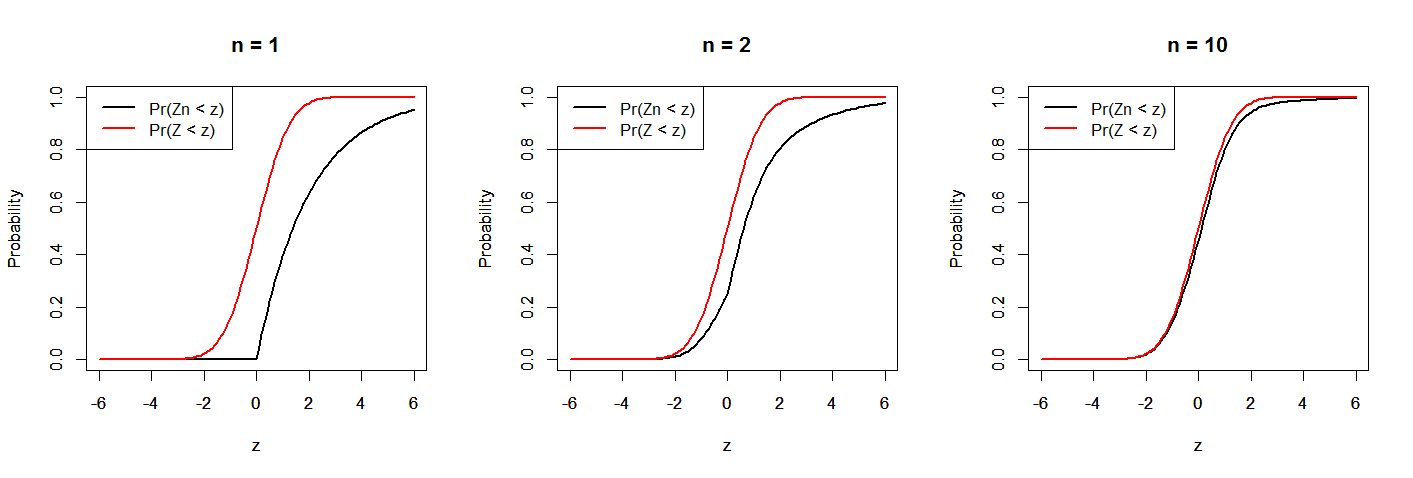
\includegraphics[width = 16cm]{probconv.png}
\end{center}


Note that convergence in probability is a stronger concept than convergence in distribution.
That is, $Z_n \overset{p}{\to} Z$ implies $Z_n \overset{d}{\to} Z$, but the converse is not true.
We formally prove the former result below.
The proof of the latter is easy by constructing a counterexample.
\begin{lemma}\label{lem:p_to_d}
	$Z_n \overset{p}{\to} Z \Longrightarrow Z_n \overset{d}{\to} Z$.
\end{lemma}

\begin{proof}
	For any positive constant $\kappa > 0$,
	\begin{align*}
	\Pr(Z_n \le z) 
	& = \Pr(Z_n \le z, \underbrace{|Z_n - Z| \le \kappa}_{Z_n - \kappa \; \le \; Z \; \le \; Z_n + \kappa}) + \Pr(Z_n \le z, |Z_n - Z| > \kappa) \\
	& \le \Pr(Z_n + \kappa \le z + \kappa, Z \le Z_n + \kappa) + \Pr(|Z_n - Z| > \kappa) \\
	& = \Pr(Z \le Z_n + \kappa \le z + \kappa) + \Pr(|Z_n - Z| > \kappa) \\
	& \le F_Z(z + \kappa) + \Pr(|Z_n - Z| > \kappa).
	\end{align*}
	Similarly,
	\begin{align*}
	F_Z(z - \kappa)
	& = \Pr(Z \le z - \kappa, \underbrace{|Z_n - Z | \le \kappa)}_{Z_n - \kappa \; \le \; Z \; \le \; Z_n + \kappa} + \Pr(Z \le z - \kappa, |Z_n - Z| > \kappa) \\
	& \le \Pr(Z \le z - \kappa, Z_n - \kappa \le Z) + \Pr(|Z_n - Z| > \kappa) \\
	& = \Pr(Z_n - \kappa \le Z \le z - \kappa) + \Pr(|Z_n - Z| > \kappa) \\
	& \le \Pr(Z_n \le z) + \Pr(|Z_n - Z| > \kappa).
	\end{align*}
	Combining these inequalities,
	\begin{align}\label{eq:ineq}
	F_Z(z - \kappa) - \Pr(|Z_n - Z| > \kappa) \le \Pr(Z_n \le z) \le F_Z(z + \kappa) + \Pr(|Z_n - Z| > \kappa).
	\end{align}
	Since $F_Z(\cdot)$ is assumed to be continuous, by choosing sufficiently small $\kappa > 0$, it holds that 
	\begin{align*}
	F_Z(z + \kappa) \le  F_Z(z) + \epsilon \\
	F_Z(z - \kappa) \ge F_Z(z) - \epsilon
	\end{align*}
	for a small $\epsilon > 0$.
	Then, taking the limit $n \to \infty$ of each term in \eqref{eq:ineq}, we have
	\[
	F_Z(z) - \epsilon \le \Pr(Z_n \le z) \le F_Z(z) + \epsilon
	\]
	with probability approaching one as $n \to \infty$. 
	Since $\epsilon$ can be made arbitrarily small, this completes the proof.
\end{proof}
\bigskip

Let $\{ X_1,\ldots,X_n \}$ be an IID sample of $X$ of size $n$ with $\E X = \mu$ and $\Var(X) = \sigma^2 < \infty$.
Then, as $n \to \infty$,
\[	
\sqrt{n}(\bar X_n - \mu) \overset{d}{\to} N(0,\sigma^2),
\]
where $N(0, \sigma^2)$ is a normal random variable with mean zero and variance $\sigma^2$; in other words,
\[
\lim_{n \to \infty}\Pr\left( \sqrt{n}(\bar X_n - \mu) \le z \right) = \frac{1}{\sqrt{2 \pi \sigma^2}}\int_{-\infty}^z \exp\left(-\frac{x^2}{2\sigma^2} \right) \mrm{d}x \;\;\; \text{for all $z\in\mathbb{R}$.}
\]
This result is known as the (Lindeberg-L\'{e}vy) \textbf{central limit theorem\index{central limit theorem}} (CLT).
The CLT states that if $n$ is sufficiently large, the distribution of $\sqrt{n}(\bar X_n - \mu)$ can be approximated by that of $N(0,\sigma^2)$.
The proof of CLT is rather complicated, and thus is omitted here.\footnote{
	In a special case where $X$ has a finite moment of any order, the proof can be greatly simplified by using the properties of the \textbf{moment generating function}.
}
\bigskip

Let $\hat\theta_n$ be an estimator of $\theta_0$ obtained from a sample of size $n$.
If $\sqrt{n}(\hat\theta_n - \theta_0) \overset{d}{\to} \mbf{N}(\mbf{0},\Omega)$, where $\mbf{N}(\mbf{0}, \Omega)$ is a multivariate normal distribution with mean vector $\mbf{0}$ and covariance matrix $\Omega$, we say that $\hat\theta_n$ is \textbf{asymptotically normally distributed\index{asymptotic normality}} at root-n rate.
$\Omega$ is called the asymptotic covariance matrix of $\sqrt{n}(\hat\theta_n - \theta_0)$.

\begin{framed}
\begin{exercise}\upshape
	Prove that $Z_n \overset{d}{\to} Z$ does not imply $Z_n \overset{p}{\to} Z$ by presenting a counterexample.
\end{exercise}

\begin{comment}
$X_0 \sim \text{Uniform}[-1,1]$, $X_n \equiv (-1)^n X_0$. 
Then $\Pr(X_n < x) = \Pr(X_0 < x)$, but $X_n$ never converges to $X_0$.
\end{comment}
\end{framed}

\section{Asymptotic properties of OLS estimator}

Consider a linear regression model:
\begin{align}\label{eq:linmodel}
	Y = X^\top \beta_0 + \eps, 
\end{align}
where $Y$ is a dependent variable, $X$ is a vector of explanatory variables, and $\eps$ is an unobserved random variable (i.e., error term) satisfying $\E[\eps \mid X] = 0$.
$\beta_0$ is the true coefficient vector to be estimated.
When the data $\{(Y_i, X_i): 1 \le i \le n\}$ are available, the \textbf{ordinary least squares\index{OLS}} (OLS) estimator $\hat \beta_n^{ols}$ of $\beta_0$ is given by
\begin{align}\label{eq:ols}
\begin{split}
	\hat \beta_n^{ols} 
	& = \argmin_{\beta} \frac{1}{n}\sum_{i = 1}^n (Y_i - X_i^\top \beta)^2 \\
	& = \left(\frac{1}{n}\sum_{i = 1}^n X_i X_i^\top \right)^{-1}\frac{1}{n}\sum_{i = 1}^n X_i Y_i,
\end{split}
\end{align}
provided that $\frac{1}{n}\sum_{i = 1}^n X_i X_i^\top$ is a nonsingular matrix. 

Here, note that the conditional expectation function $\E[Y \mid X]$ is a minimizer of the \textbf{mean squared error\index{MSE}} (MSE) among all possible regression functions:
\begin{align}\label{eq:msemin}
	\E[Y \mid X] = \argmin_{g \in \mcl{G}} \E[(Y - g(X))^2],
\end{align}
where $\mcl{G}$ is the set of all measurable functions of $X$.
Since we have assumed that $\E[\eps \mid X] = 0 $ (i.e., $\E [Y \mid X] = X^\top \beta_0$), we can restrict the above MSE minimization with respect to the class of linear functions of $X$:
\begin{align*}
	\beta_0 
	& = \argmin_{\beta \in \mbb{R}^{\text{dim}(X)}} \E[(Y - X^\top \beta)^2]\\
	& = \E[XX^\top]^{-1} \E[XY].
\end{align*} 
Thus, we can see that the OLS objective function in \eqref{eq:ols} is the sample analog of the population MSE, and that the estimated regression function, say $\hat g_n(X) \equiv X^\top \hat \beta_n^{ols}$, is an estimator of $\E[Y \mid X]$.\footnote{\label{foot:ols_moment}
	Another interpretation of the OLS estimator is that it is a sample solution to the moment equation $\E[Y \mid X] = X^\top\beta$.
	Premultiplying $X$ on both sides of this equation and taking the expectation yield
	\begin{align*}
		\E[X \E[Y \mid X]] = \E[XX^\top]\beta_0
		& \iff \E[XY] = \E[XX^\top]\beta_0 \\
		& \iff \beta_0 = \E[XX^\top]^{-1}\E[XY].
	\end{align*}
	Note that, in the above characterization of $\beta_0$, the multiplier does not need to be $X$.
	As easily confirmed, for any general $h(X)$, we can obtain $\beta_0 = \E[h(X)X^\top]^{-1}\E[h(X)Y]$ as long as $\E[h(X)X^\top]$ exists and is nonsingular.
	}
	By \eqref{eq:linmodel}, we can rewrite the right-hand side of \eqref{eq:ols} as
\begin{align*}
	\hat \beta_n^{ols} 
	& = \left(\frac{1}{n}\sum_{i = 1}^n X_i X_i^\top \right)^{-1}\frac{1}{n}\sum_{i = 1}^n X_i (X_i^\top\beta_0 + \eps_i) \\
	& = \beta_0 + \left(\frac{1}{n}\sum_{i = 1}^n X_i X_i^\top \right)^{-1}\frac{1}{n}\sum_{i = 1}^n X_i \eps_i.
\end{align*}

\paragraph{Proof of consistency}

To prove the consistency of $\hat \beta_n^{ols}$, it is sufficient to show that
\begin{align}\label{eq:convzero}
	\left(\frac{1}{n}\sum_{i = 1}^n X_i X_i^\top \right)^{-1}\frac{1}{n}\sum_{i = 1}^n X_i \eps_i \overset{p}{\to} \mbf{0}.
\end{align}
Assume that the data are IID and that $\E[XX^\top]$ exists and is nonsingular.
Then, by WLLN, $\frac{1}{n}\sum_{i = 1}^n X_i X_i^\top \overset{p}{\to} \E[XX^\top]$ element-wisely.
Further, by the continuity of matrix inversion, we can show that $\left(\frac{1}{n}\sum_{i = 1}^n X_i X_i^\top \right)^{-1} \overset{p}{\to} \E[XX^\top]^{-1}$.
In addition, it holds that $\frac{1}{n}\sum_{i = 1}^n X_i \eps_i \overset{p}{\to} \mbf{0}$ since
\[
	\E[X_i \eps_i ] = \E[X_i \E[\eps_i \mid X_i]] = \mbf{0}
\]
by the law of iterated expectations (LIE) and $\E[\eps_i \mid X_i] = 0$.
Finally, we can prove \eqref{eq:convzero} by Lemma \ref{lem:prodconv}.

\paragraph{Proof of root-n-consistency}

Suppose that $\E[\eps^2 \mid X ] = \sigma^2 < \infty$ (i.e., \textbf{homoskedasticity\index{homoskedasticity}}) for simplicity.
Write
\begin{align*}
	\sqrt{n}(\hat \beta_n^{ols} - \beta_0) 
	& = \left(\frac{1}{n}\sum_{i = 1}^n X_i X_i^\top \right)^{-1}\frac{1}{\sqrt{n}}\sum_{i = 1}^n X_i \eps_i\\
	& = \left(\mbf{X}_n^\tr \mbf{X}_n/n\right)^{-1}\mbf{X}_n^\tr\mcl{E}_n/\sqrt{n},
\end{align*}
where $\mbf{X}_n = (X_1, \ldots, X_n)^\tr$, and $\mcl{E}_n = (\eps_1, \ldots, \eps_n)^\tr$.
The independence and homoskedasticity assumptions imply that $\E[\mcl{E}_n\mcl{E}_n^\tr \mid \{X_i\}_{i=1}^n] = \sigma^2 I_n$.
Hence,
\begin{align*}
	\E\left[||\sqrt{n}(\hat \beta_n^{ols} - \beta_0)||^2 \mid \{X_i\}_{i=1}^n \right]
	& = \text{trace}\left\{\left(\mbf{X}_n^\tr \mbf{X}_n/n\right)^{-1}\mbf{X}_n^\tr \E[\mcl{E}_n\mcl{E}_n^\tr \mid \{X_i\}_{i=1}^n] \mbf{X}_n \left(\mbf{X}_n^\tr \mbf{X}_n/n\right)^{-1}\right\}/n \\
	& = \sigma^2 \text{trace}\left\{\left(\mbf{X}_n^\tr \mbf{X}_n/n\right)^{-1}\right\} = O(\text{dim}(X)).
\end{align*}
Then, by Markov's inequality, $||\sqrt{n}(\hat \beta_n^{ols} - \beta_0)|| = O_P(1)$.

\paragraph{Proof of asymptotic normality}

By $\left(\frac{1}{n}\sum_{i = 1}^n X_i X_i^\top \right)^{-1} \overset{p}{\to} \E[XX^\top]^{-1}$ and Slutsky's theorem \ref{lem:slutsky}, the asymptotic distribution of  $\sqrt{n}(\hat \beta_n^{ols} - \beta_0)$ is equal to that of $\E[XX^\top]^{-1}\frac{1}{\sqrt{n}}\sum_{i = 1}^n X_i \eps_i$.
The mean of $\frac{1}{\sqrt{n}}\sum_{i = 1}^n X_i \eps_i$ is zero, and the variance of it is
\begin{align*}
	\Var\left(\frac{1}{\sqrt{n}}\sum_{i = 1}^n X_i \eps_i\right) 
	= \E\left[ \frac{1}{n}\sum_{i = 1}^n\sum_{j = 1}^n X_i X_j^\top \eps_i \eps_j \right]
	& = \E\left[ \frac{1}{n}\sum_{i = 1}^n X_iX_i^\top \eps^2_i \right]\\
	& = \sigma^2 \frac{1}{n}\sum_{i = 1}^n  \E[  X_iX_i^\top ] = \sigma^2 \E[  XX^\top ],
\end{align*}
where the second equality follows by the independence assumption, and the third equality is by LIE and the homoskedasticity assumption.
Hence, by CLT, we have
\[
	\frac{1}{\sqrt{n}}\sum_{i = 1}^n X_i \eps_i \overset{d}{\to} \mbf{N}(\mbf{0}, \sigma^2 \E[XX^\top]),
\]
implying that 
\[
	\sqrt{n}(\hat \beta_n^{ols} - \beta_0) \overset{d}{\to} \mbf{N}(\mbf{0}, \sigma^2 \E[XX^\top]^{-1}).
\]

\begin{framed}
\begin{exercise}\upshape
	Prove \eqref{eq:msemin}.
\end{exercise}
\begin{exercise}\upshape
	Suppose now that the error term is heteroskedastic in the following sense: $\E[\eps^2 \mid X] = \sigma^2(X)$.
	Derive the asymptotic distribution of $\sqrt{n}(\hat \beta_n^{ols} - \beta_0)$.
\end{exercise}
\begin{exercise}\upshape
	Consider a linear regression model:
	\[
	Y = X^\top \beta_0 + \eps,
	\]
	where $\E[\eps \mid X] = 0$.
	Define the \textbf{ridge regression} estimator:
	\[
	\hat \beta_n^{ridge} \equiv \left(\frac{1}{n}\sum_{i = 1}^n X_i X_i^\top + \lambda I_{\text{dim}(X)} \right)^{-1}\frac{1}{n}\sum_{i = 1}^n X_i Y_i,
	\]
	where $\lambda$ is a given positive number.
	Prove that (1) $\hat \beta_n^{ridge}$ is a biased estimator of $\beta_0$, and that (2) if $\lambda \to 0$, $\hat \beta_n^{ridge}$ is consistent for $\beta_0$.
\end{exercise}
\end{framed}

%%%%%%%%%%%%%%%%%%%%%%%%%%%%%%%%%%%%%%%%%%%%%%%%%%%%%%%%%%%%
%%%%%%%%%%%%%%%%%%%%%%%%%%%%%%%%%%%%%%%%%%%%%%%%%%%%%%%%%%%%
%%%%%%%%%%%%%%%%%%%%%%%%%%%%%%%%%%%%%%%%%%%%%%%%%%%%%%%%%%%%

\chapter{Two-Stage Least Squares}\label{chap:2sls}
\section{Endogeneity and exogeneity}

Consider the following simple regression model:
\begin{align}\label{eq:simple}
Y = \beta_0 + X\beta_1 + \eps,
\end{align}
where $Y$ is a dependent variable, $X$ is a scalar explanatory variable, and $\eps$ is an unobserved error term satisfying $\E \eps = 0$.
$\beta_0$ and $\beta_1$ are unknown parameters to be estimated.
Taking the expectation of both sides of \eqref{eq:simple}, we obtain $\beta_0 = \E Y - \E [X] \beta_1$.
Then, the model \eqref{eq:simple} can be rewritten as
\begin{align}\label{eq:simplediff}
Y - \E Y = (X - \E X)\beta_1 + \eps.
\end{align}
Further, premultiplying both sides of \eqref{eq:simplediff} by $X$ and taking the expectation of them yield
\[
\underbrace{\E[X(Y - \E Y)]}_{\Cov(X,Y)} = \underbrace{\E[X (X - \E X)]}_{\Var(X)} \beta_1 + \underbrace{\E[X \eps]}_{\Cov(X, \eps)}.
\]
Assuming that $\Var(X) > 0$, divide the above equation by $\Var(X)$ to obtain
\begin{align}\label{eq:beta1}
\frac{\Cov(X,Y)}{\Var(X)} = \beta_1 + \frac{\Cov(X,\eps)}{\Var(X)}.
\end{align}
Notice that the sample analog of the left-hand side of \eqref{eq:beta1} is exactly the OLS estimator of the slope parameter $\beta_1$, and under standard conditions we have
\[
	\hat \beta_{n1}^{ols} \overset{p}{\to} \beta_1 + \frac{\Cov(X,\eps)}{\Var(X)}.
\]
This implies that the OLS estimator $\hat \beta_{n1}^{ols} $ cannot correctly (i.e., consistently) estimate $\beta_1$ if $\Cov(X, \eps) \neq 0$.
When $\Cov(X, \eps) = 0$ holds true, we say that $X$ is \textbf{exogenous\index{exogeneity}}.
If it is not satisfied, we say that $X$ is \textbf{endogenous\index{endogeneity}}.
\[
\begin{array}{ll}
\text{Exogeneity:} & \hspace{-5pt}\text{$X$ is uncorrelated with the error term $\eps$.} \\
\text{Endogeneity:} & \hspace{-5pt}\text{$X$ is correlated with the error term $\eps$.} \\
\end{array}
\]
Under exogeneity, the parameter $\beta_1$ can be characterized simply by 
\begin{equation*}
	\beta_1 = \frac{\Cov(X, Y)}{\Var(X) }.
\end{equation*}
On the other hand, if $X$ is endogenous, $\Cov(X, Y)/\Var(X)$ entails a bias, so-called \textbf{endogeneity bias\index{endogeneity bias}}, that amounts to $\Cov ( X, \eps )/\Var(X)$.
In general, the magnitude and even the sign of the endogeneity bias are uncertain because $\eps$ is unobservable.
Hence, in the presence of endogeneity, the OLS estimator is inconsistent, and thus the OLS estimate is uninformative about the true impact of $X$ on $Y$.
\bigskip

There are many potential sources of endogeneity.
The two most important sources are from \textbf{omitted variables\index{omitted variables}} and from \textbf{simultaneity\index{simultaneity}}. 

\paragraph{Omitted variables}
Consider the following multiple regression model with two explanatory variables $X_1$ and $X_2$:
\begin{align}\label{eq:multiple}
Y = \beta_0 + X_1 \beta_1 + X_2 \beta_2 + \eps.
\end{align}
Here, we assume that both $X_1$ and $X_2$ are exogenous: $\E[ X_1 \eps ] = \E [ X_2 \eps ] = 0$.
Then, when both $X_1$ and $X_2$ are observable, the slope parameters  $\beta_1$ and $\beta_2$ can be consistently estimated simply by regressing $Y$ on $(X_1, X_2)$.

Now consider a case in which $X_2$ is unobservable for some reason.
Excluding unobservable $X_2$ from the model \eqref{eq:multiple}, we regress $Y$ only on $X_1$ based on the following simple regression model:
\begin{align}\label{eq:simple2}
Y = \alpha +X_1 \beta_1 + \eta, 
\end{align}
where $\alpha = \beta_0 + \E[ X_2 ] \beta_2$, and $\eta$ is a new error term defined by
\[
\eta = ( X_2 - \E X_2  ) \beta_2 + \eps
\]
such that $\E\eta = 0$.
In this simple regression model, the explanatory variable $X_2$, which needs to be included in the model if $\beta_{2}\neq 0$, is omitted from the analysis. 
In order to correctly estimate $\beta_1$ based on the model \eqref{eq:simple2}, $X_1$ needs to be an exogenous variable in the sense that	$\E[ X_1 \eta ]  = 0$.
However, by the definition of $\eta$,
\begin{align*}
	\E[  X_1 \eta ]   
	& = \E\left[  X_1 \left(  X_2 - \E X_2   \right) \beta_2 + X_1 \eps \right] \\
	& = \Cov( X_1, X_2)  \beta_2 + \Cov( X_1, \eps)\\
	& = \Cov( X_1, X_2)  \beta_2.
\end{align*}
Hence, unless either $\Cov( X_1, X_2 ) = 0$ or $\beta_2 = 0$ (or both), $X_1$ is an endogenous variable in the model \eqref{eq:simple2}: $\E[X_1 \eta] \neq 0$.

\paragraph{Simultaneity}
As an example, consider estimating the effect of police on crime.
Let $X_i$ be the number of police officers in a district $i$ and $Y_i$ be the number of crime incidents in this district. 
It is expected that there exists a ``simultaneity" between police and crime; that is, if crime rate increases, a larger police force will be needed, at the same time, increasing police force reduces crime.
This relationship can be expressed as: 
\begin{align*}
Y_i  &  =\beta_0 + X_i \beta_1 + \eps_i \;\; \text{ ($\beta_1$: \# of  police officers $\rightarrow$ \# of crimes)} \\
X_i  &  =\gamma_0 + Y_i\gamma_1 + u_i \;\;\; \text{ ($\gamma_1$: \# of crimes $\rightarrow$ \# of police officers)},
\end{align*}
where $(\gamma_0, \gamma_1)$ is another set of unknown parameters, and $u$ is an unobserved error term.
For simplicity of discussion, we do not consider other factors that may influence on $Y$ and $X$.
If $X_i$ is an endogenous variable such that $\E[  X_i \eps_i ]  \neq 0$, simply regressing $Y_i$ on $X_i$ does not give us a consistent estimator of $\beta_1$.

According to the second model,
\begin{align*}
	\E[ X_i \eps_i ] 
	& = \E[(\gamma_0 + Y_i \gamma_1 + u_i) \eps_i ] \\
	& = \E[  Y_i \eps_i ]  \gamma_1 + \E[u_i \eps_i].
\end{align*}
For the second term on the right-hand side, if there are unobservable regional factors that can affect both $X$ and $Y$, we would have $\E[u_i \eps_i] \neq 0$.
Further, the first term is necessarily non-zero as long as $\gamma_1 \neq 0$ (i.e., simultaneity exists) because
\begin{align*}
	\E[  Y_i \eps_i ]
	& = \E[(\beta_0 + X_i \beta_1 + \eps_i) \eps_i ] \\
	& = \E[  X_i \eps_i ]  \beta_1 + \underbrace{\E[\eps^2_i]}_{ > \: 0}.
\end{align*}
Thus, endogeneity problem arises when simultaneity exists.

\begin{figure}[h!]
	\begin{center}
		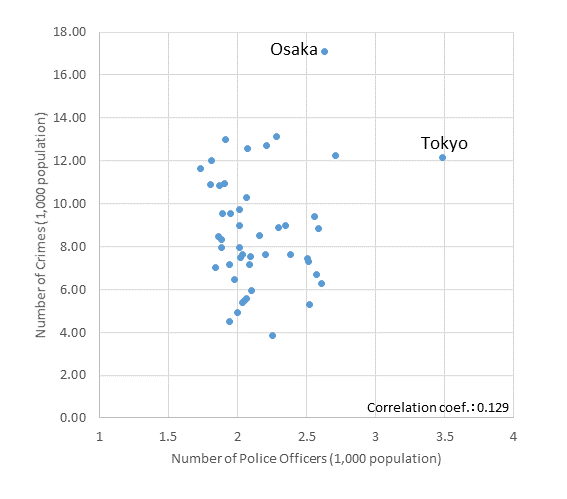
\includegraphics[width = 10.6cm]{polcrime.png}
		\caption{Simultaneity between police and crime.}
	\end{center}
\end{figure}

\begin{framed}
\begin{exercise}\upshape
	Give specific examples of endogeneity bias caused by (1) omitted variables and (2) simultaneity (other than those mentioned above).
\end{exercise}
\end{framed}

\section{Instrumental variables}

A common approach to account for the endogeneity problem is to use \textbf{instrumental variables\index{instrumental variables}} (IV).
Again, consider the following simple regression model: 
\[
	Y = \beta_0 + X \beta_1 + \eps.
\]
Here, we assume that $X$ is endogenous: $\E[X\eps] \neq 0$.
An instrumental variable for $X$, which we denote by $Z$, is a random variable that satisfies the following conditions:
\[
\begin{array}{ll}
	\E[Z \eps] = \Cov(Z, \eps) = 0 & \textbf{Exclusion restriction\index{exclusion restriction}} \\
	\Cov(Z, X) \neq 0 & \textbf{Relevance condition\index{relevance condition}}
\end{array}
\]
The exclusion restriction says that the instrumental variable $Z$ is uncorrelated with the error term $\eps$.
This implies that $Z$ is not a direct determinant of $Y$; if $Z$ directly affects $Y$, the information about $Z$ must be contained in $\eps$, leading to a correlation of $Z$ and $\eps$ (this is why the condition is called ``exclusion" restriction).
The relevance condition requires that the instrumental variable $Z$ is a determinant of the endogenous variable $X$.

\begin{example}\upshape
	As a typical econometric application, suppose that $Y$ is an individual's wage and $X$ is his education in years.
	It would be expected that the higher the individual's ability, the higher his wage.
	However, since one's ability is hard to measure correctly, the effect of ability on $Y$ will be partly included in the error term $\eps$.
	Also, there must exist a positive correlation between one's ability and education.
	Consequently, a positive correlation between $X$ and $\eps$ arises naturally; that is, $X$ should be treated as an endogenous variable.
	Here, let $Z$ be the individual's parents' education level.
	It would be legitimate to suppose that the parents' education does not ``directly" affect his own wage $Y$ (but influences on $Y$ only through $X$), and it is surely correlated with his education level.
	Thus, the parents' education level can be a valid instrument for $X$.
\end{example}

\begin{example}\upshape
	Consider once again the simultaneous relationship of police and crime.
	Here, let $Y_{it}$ and $X_{it}$ be the number of crime incidents and the size of police force in city $i$ year $t$, respectively.
	As an instrumental variable for $X_{it}$, \cite{levitt1997using} employed an indicator variable $Z_{it}$ which takes one if $t$ is the mayoral election year in city $i$.
	In years when there is an election, the incumbent mayors would have an incentive to increase the police force to reduce crime (which was indeed confirmed as statistically significant in \cite{levitt1997using}).
	Also, the presence of elections should not have ``direct'' impacts on the number of crimes.
	Thus, $Z_{it}$ is considered to be a valid instrument for $X_{it}$. 
\end{example}

Now, suppose that we have a valid instrumental variable $Z$ satisfying both the exclusion restriction and relevance condition.
Then, premultiplying both sides of \eqref{eq:simplediff} by $Z$ and taking the expectation of them yield
\[
	\underbrace{\E[Z (Y - \E Y)]}_{\Cov(Z, Y)} = \underbrace{\E[Z (X - \E X)]}_{\Cov(Z, X) \neq 0} \beta_1 + \underbrace{\E[Z \eps]}_{\Cov(Z, \eps) = 0}.
\]
Thus, we obtain
\[
	\beta_1 = \frac{\Cov(Z, Y)}{\Cov(Z, X)}.
\]
Here, suppose that the sample $\{(Y_i, X_i, Z_i): 1 \le i \le n\}$ is available, and let $\hat{\Cov}_n(Z, Y)$ and $\hat{\Cov}_n(Z, X)$ be the sample covariances of $(Z, Y)$ and $(Z, X)$, respectively.
Then, the above result implies that $\beta_1$ can be estimated by
\[
	\hat{\beta}_{n1} \equiv \frac{\hat{\Cov}_n(Z, Y)}{\hat{\Cov}_n(Z, X)}.
\] 
Further, note that 
\begin{align*}
	\hat{\Cov}_n(Z, Y) 
	& = \frac{1}{n}\sum_{i = 1}^n Z_i (Y_i - \bar Y_n) \\
	& = \frac{1}{n}\sum_{i = 1}^n Z_i ((\beta_0 + X_i\beta_1 + \eps_i) - (\beta_0 + \bar X_n \beta_1 + \bar \eps_n))\\ 
	& =\frac{1}{n}\sum_{i = 1}^n Z_i ((X_i - \bar X_n) \beta_1 + (\eps_i - \bar \eps_n))\\ 
	& = \hat{\Cov}_n(Z, X)\beta_1 + \hat{\Cov}_n(Z, \eps),
\end{align*}
where $\bar Y_n$, $\bar X_n$, and $\bar \eps_n$ are the sample averages of $Y$, $X$, and $\eps$, respectively.
Hence, 
\begin{align}\label{eq:weakIV}
	\hat{\beta}_{n1} = \beta_1 + \frac{\hat{\Cov}_n(Z, \eps)}{\hat{\Cov}_n(Z, X)}.
\end{align}
The second term on the right-hand side of \eqref{eq:weakIV} is the finite sample estimation bias.\footnote{
	Thus, this IV-based estimator is not an unbiased estimator.
}
If $\Cov(Z,X)$ is close to zero, i.e., if $Z$ is almost irrelevant to $X$, $\hat{\Cov}_n(Z, X)$ is also close to zero.
Thus, in this case, the estimation bias of $\hat{\beta}_{n1}$ can be very large.
This problem is known as the \textbf{weak instruments problem\index{weak instruments problem}}. 
There are several formal tests for weak instruments (see, e.g., \cite{stock2005testing}); however, the details are omitted here.

\begin{framed}
\begin{exercise}\upshape
	Suppose that we would like to estimate the causal impact of aircraft noise on land prices by a simple regression analysis.
	In this regression model, we should suspect that the aircraft noise variable is endogenous. Explain why, and give an example of a valid instrumental variable in this analysis.
\end{exercise}
\end{framed}

\section{2SLS procedure}

In the following, we consider a more general case with multiple regressors and multiple instrumental variables:
\begin{align*}
	Y = D \cdot \alpha_0 + X^\tr \beta_0 + \eps,
\end{align*}
where $X = (X_1, \ldots , X_{d_x})^\tr$ is a vector of exogenous explanatory variables (including a constant term), and $D$ is an endogenous explanatory variable.
Suppose that we have a vector of instrumental variables $Z_1 = (Z_{11}, \ldots, Z_{1d_z})^\tr$ for $D$.

We modify the above estimation procedure for a simple regression model as follows.
First, let $Z = (Z_1^\tr, X^\tr)^\tr$ be a vector of all exogenous variables, and assume that the inverse matrix $\E[Z Z^\tr]^{-1}$ exists.
Further, let $\mcl{P}_Z(A)$ be the orthogonal projection of $A$ onto $Z$; that is, $\mcl{P}_Z(A) \equiv Z^\tr \E[ZZ^\tr]^{-1}\E[Z A]$.
When $A$ is a vector $A = (A_1, \ldots A_k)^\tr$, $\mcl{P}_Z(A)$ is defined as 
\[
	\mcl{P}_Z(A) = (Z^\tr \E[Z Z^\tr]^{-1} \E[ZA_1], \ldots , Z^\tr \E[Z Z^\tr]^{-1} \E[ZA_k])^\tr.
\]
Rewrite the model as follows:
\begin{align}\label{eq:projection}
\begin{split}
	Y 
	& = \mcl{P}_Z(D) \cdot \alpha_0 + X^\tr \beta_0 +u \\
	& = \mcl{P}_Z(H)^\tr \theta_0 +u ,
\end{split}
\end{align}
where $H = (D, X^\tr)^\tr$, $\theta_0 = (\alpha_0, \beta_0^\tr)^\tr$, and $u = (D - \mcl{P}_Z(D)) \cdot \alpha_0 + \eps$.
The second equality in \eqref{eq:projection} is due to the fact that $\mcl{P}_Z(X) = X$ (see the supplementary material in this chapter).
By the exclusion restriction and \eqref{eq:ZX} below, we can find that 
\begin{align*}
	\E[\mcl{P}_Z(H) u] 
	& = \E\left[
	\begin{array}{c}
	\mcl{P}_Z(D) u \\
	X u
	\end{array}
	\right] \\
		& = \E\left[
	\begin{array}{c}
	\mcl{P}_Z(D) (D - \mcl{P}_Z(D))  \\
	X (D - \mcl{P}_Z(D))
	\end{array}
	\right] \cdot \alpha_0  = \underset{(1 + d_x) \times 1}{\mbf{0}}.
\end{align*}
This result implies that $\theta_0$ can be estimated by the least squares regression of $Y$ on $(\mcl{P}_Z(D), X)$, or equivalently, on $\mcl{P}_Z(H)$.
Figure \ref{fig:geo2sls} provides a simple geometry of the above discussion.

\begin{figure}[h!]
	\begin{center}
		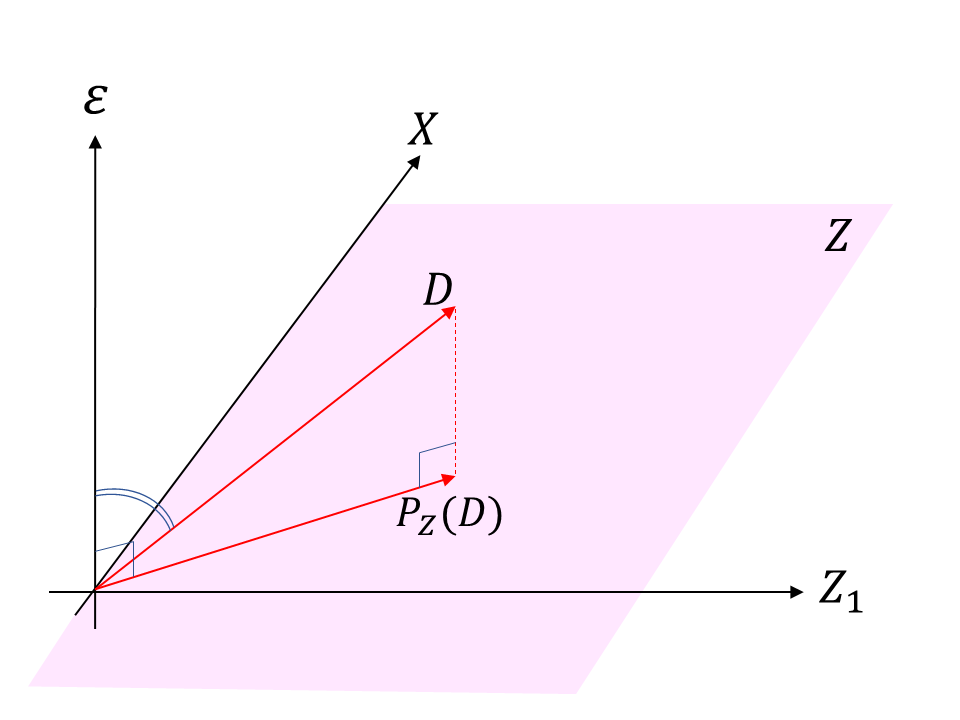
\includegraphics[width = 9cm]{projection.png}
		\caption{Orthogonal projection of $D$ onto $Z = (Z_1, X)$.}
		\label{fig:geo2sls}
	\end{center}
\end{figure}

Now, suppose that we have data of $n$ observations $\{(Y_i, D_i, X_i, Z_{1i}): 1 \le i \le n\}$.
For a sample analog to the above procedure, the parameter $\theta_0$ can be estimated in the following two steps:

\textbf{Step (1)}: perform a least squares regression of $D$ on $Z = (Z_1^\tr, X^\tr)^\tr$, and compute the predicted value of $D$ by $\hat D = Z^\tr \hat\gamma_n$, where
\[
\hat\gamma_n \equiv \left( \frac{1}{n}\sum_{i=1}^n Z_i Z_i^\tr \right)^{-1}\frac{1}{n}\sum_{i=1}^n Z_i D_i. 
\]
(At this step, it is important to check the significance of $\hat \gamma_n$.
If all elements of $\hat\gamma_n$ are close to zero, the weak instruments problem can occur.)
Let $\hat H = (\hat D, X^\tr)^\tr$.

\textbf{Step (2)}: perform a least squares regression of $Y$ on $\hat H$ to estimate $\theta_0$:
\[
	\hat\theta_n^{2sls} \equiv \left( \frac{1}{n}\sum_{i=1}^n \hat H_i \hat H_i^\tr \right)^{-1}\frac{1}{n}\sum_{i=1}^n \hat H_i Y_i.
\]
The above estimation procedure is called the \textbf{two-stage least squares\index{two-stage least squares}} (2SLS) estimator.

Noting the second equality in \eqref{eq:projection}, the 2SLS estimator can be, in fact, implemented in one step.
To do so, we introduce the following matrix notations: $\mbf{Y}_n = (Y_1, \ldots , Y_n)^\tr$, $\mbf{D}_n = (D_1, \ldots, D_n)^\tr$, $\mbf{X}_n = (X_1, \ldots, X_n)^\tr$, $\mbf{Z}_n = (Z_1, \ldots, Z_n)^\tr$, and $\mbf{H}_n = (H_1, \dots , H_n)^\tr$.
Further, let $\mcl{P}_{\mbf{Z}_n}$ be an empirical projection matrix, which is defined by
\[
	\mcl{P}_{\mbf{Z}_n} \equiv \mbf{Z}_n(\mbf{Z}_n^\tr \mbf{Z}_n)^{-1} \mbf{Z}_n^\tr.
\]
Then, $\hat{\mbf{D}}_n = (\hat D_1, \ldots , \hat D_n)^\tr$ is obtained by $\hat{\mbf{D}}_n = \mcl{P}_{\mbf{Z}_n} \mbf{D}_n$.
In addition, by the same argument as the fact $\mcl{P}_Z(X) = X$, we can easily see that $\mbf{X}_n = \mcl{P}_{\mbf{Z}_n} \mbf{X}_n$.
Therefore, $\hat{\mbf{H}}_n \equiv [\hat{\mbf{D}}_n \; ; \; \mbf{X}_n] = \mcl{P}_{\mbf{Z}_n}\mbf{H}_n$.
Consequently, noting the fact that $\mcl{P}_{\mbf{Z}_n}\mcl{P}_{\mbf{Z}_n} = \mcl{P}_{\mbf{Z}_n}$,\footnote{This property is called \textit{idempotency}.} the 2SLS estimator $\hat\theta_n^{2sls}$ can be numerically equivalently expressed as 
\begin{align}\label{eq:2slsMat}
	\begin{split}
	\hat\theta_n^{2sls}
	& = \left(\hat{\mbf{H}}_n^\tr \hat{\mbf{H}}_n \right)^{-1} \hat{\mbf{H}}_n^\tr \mbf{Y}_n\\
	& = \left(\mbf{H}_n^\tr \mcl{P}_{\mbf{Z}_n} \mcl{P}_{\mbf{Z}_n} \mbf{H}_n \right)^{-1} \mbf{H}_n^\tr \mcl{P}_{\mbf{Z}_n} \mbf{Y}_n \\
	& = \left(\mbf{H}_n^\tr  \mbf{Z}_n(\mbf{Z}_n^\tr \mbf{Z}_n)^{-1} \mbf{Z}_n^\tr \mbf{H}_n \right)^{-1} \mbf{H}_n^\tr  \mbf{Z}_n(\mbf{Z}_n^\tr \mbf{Z}_n)^{-1} \mbf{Z}_n^\tr \mbf{Y}_n.
	\end{split}
\end{align}

\section{Asymptotic properties}\label{sec:2slsAsymptotics}

The asymptotic properties of the 2SLS estimator \eqref{eq:2slsMat} can be relatively easily derived.
First, noting that $\mbf{Y}_n = \mbf{H}_n^\top\theta_0 + \mcl{E}_n$, where $\mcl{E}_n = (\eps_1, \ldots , \eps_n)^\tr$, we can obtain
\begin{align*}
	\hat\theta_n^{2sls} 
	& = \theta_0 + \left[\mbf{H}_n^\top \mbf{Z}_n(\mbf{Z}_n^\top \mbf{Z}_n)^{-1}\mbf{Z}_n^\top \mbf{H}_n  \right]^{-1}\mbf{H}_n^\top \mbf{Z}_n(\mbf{Z}_n^\top \mbf{Z}_n)^{-1}\mbf{Z}_n^\top\mcl{E}_n.
\end{align*}
by WLLN, under standard conditions, we have $\mbf{H}_n^\top \mbf{Z}_n/n \overset{p}{\to} \E[H Z^\tr]$,  $\mbf{Z}_n^\tr \mbf{Z}_n/n \overset{p}{\to} \E[Z Z^\tr]$, and  $\mbf{Z}_n^\tr \mcl{E}_n/n \overset{p}{\to} \E[Z \eps] = \underset{(d_z + d_x)\times 1}{\mbf{0}}$ as the sample size increases to infinity.
Thus,
\begin{align*}	
	\hat\theta_n^{2sls} - \theta_0
	& = \left[(\mbf{H}_n^\top \mbf{Z}_n/n)(\mbf{Z}_n^\top \mbf{Z}_n/n)^{-1}(\mbf{Z}_n^\top \mbf{H}_n/n ) \right]^{-1}(\mbf{H}_n^\top \mbf{Z}_n/n)(\mbf{Z}_n^\top \mbf{Z}_n/n)^{-1}(\mbf{Z}_n^\top\mcl{E}_n/n) \\
	& \overset{p}{\to} \left[ \E[H Z^\tr] \E[Z Z^\tr]^{-1} \E[Z H^\tr] \right]^{-1} \E[H Z^\tr] \E[Z Z^\tr]^{-1} \underbrace{\E[Z \eps]}_{= \; \mbf{0}} = \mbf{0}
\end{align*}
by Lemma \ref{lem:prodconv} and the continuous mapping theorem, implying that the 2SLS estimator $\hat\theta_n^{2sls}$ is consistent for $\theta_0$.

Next, suppose for simplicity that the error terms $\eps_i$'s are IID with variance $\E[\eps^2] = \sigma^2$.
Further, assume that $\eps$ is independent of $Z$ (note that this is a stronger condition than the uncorrelation between $\eps$ and $Z$).
Then, by CLT, it would hold that $\mbf{Z}_n^\top\mcl{E}_n/\sqrt{n} \overset{d}{\to} \mbf{N}(\mbf{0}, \E[Z Z^\tr]\sigma^2)$.
Hence, by Slutsky's theorem \ref{lem:slutsky}, we obtain the asymptotic normality of $\sqrt{n}(\hat\theta_n^{2sls} - \theta_0)$ as follows:
\begin{align*}
	\sqrt{n}(\hat\theta_n^{2sls} - \theta_0) 
	& = \left[(\mbf{H}_n^\top \mbf{Z}_n/n)(\mbf{Z}_n^\top \mbf{Z}_n/n)^{-1}(\mbf{Z}_n^\top \mbf{H}_n/n ) \right]^{-1}(\mbf{H}_n^\top \mbf{Z}_n/n)(\mbf{Z}_n^\top \mbf{Z}_n/n)^{-1}\mbf{Z}_n^\top\mcl{E}_n/\sqrt{n} \\
	& \overset{d}{\to} \mbf{N}\left(\mbf{0}, \sigma^2  \left[ \E[H Z^\tr] \E[Z Z^\tr]^{-1} \E[Z H^\tr] \right]^{-1}\right).
\end{align*}

\begin{framed}
\begin{exercise}\upshape
	Explain what happens if we create $\hat D$ using only $Z_1$ without $X$ and perform a 2SLS estimation.
	Is such an estimator consistent? If yes, prove that, and if no, explain under what additional condition(s) the estimator becomes consistent.
\end{exercise}
\end{framed}

\section{Durbin-Wu-Hausman test for endogeneity}

Note that the 2SLS estimator is consistent and asymptotically normal even when the variable $D$ is in fact exogenous. 
Of course, if $D$ is an exogenous variable, we can use the OLS estimator, and, in general, the OLS estimator is more efficient than the 2SLS estimator when both estimators are available.
Thus, statistically testing the appropriateness of using OLS or the necessity of using 2SLS is useful.

Here, we consider the following null hypothesis
\[
	\mbb{H}_0: \Cov(D, \eps) = 0,
\]
and the alternative hypothesis is its negation
\[
	\mbb{H}_1: \Cov(D, \eps) \neq 0.
\]
Under the null hypothesis $\mbb{H}_0$, both OLS and 2SLS estimators of $\alpha_0$, say $\hat \alpha_n^{ols}$ and $\hat \alpha_n^{2sls}$, respectively,  are consistent and asymptotically normal.
However under $\mbb{H}_1$, the OLS estimator $\hat \alpha_n^{ols}$ converges to $\alpha_0 + \text{endogeneity bias}$, while the 2SLS estimator is still consistent for $\alpha_0$.
Thus the difference between the OLS and 2SLS estimators is a valid test statistic for endogeneity. 

Suppose that $\mbb{H}_0$ is true.
Then, since both $\hat \alpha_n^{ols}$ and $\hat \alpha_n^{2sls}$ are asymptotically distributed as normal, we can show that the difference of them $\hat \alpha_n^{ols} - \hat \alpha_n^{2sls}$ is also asymptotically normal.
Thus, letting 
\[
	T_n \equiv \frac{\hat \alpha_n^{ols} - \hat \alpha_n^{2sls}}{\sqrt{\Var(\hat \alpha_n^{ols} - \hat \alpha_n^{2sls})}},
\]	
we have $T_n \overset{d}{\to} N (0,1)$ and also $T_n^2 \overset{d}{\to} \chi^2(1)$ under $\mbb{H}_0$, where $\chi^2(1)$ denotes the chi-square distribution with one degree of freedom.
Thus, if $T_n^2 > 3.841\ldots$ for instance, we can reject $\mbb{H}_0$ at the 5\% significance level.

In a more general setting where $q$ endogenous regressors $D = (D_1, \ldots, D_q)^\top$ exist, the statistic $T_n$ can be defined as $T_n \equiv \left[\Cov(\hat \alpha_n^{ols} - \hat \alpha_n^{2sls})\right]^{-1/2}(\hat \alpha_n^{ols} - \hat \alpha_n^{2sls})$, and it holds that $T_n^\top T_n \overset{d}{\to} \chi^2(q)$.
The above testing procedure for endogeneity is called the \textbf{Durbin-Wu-Hausman test\index{Durbin-Wu-Hausman test}}.

 
\section{A causal interpretation of the 2SLS estimate}

In this section, for simplicity, suppose that we have a dummy endogenous variable $D \in \{0,1\}$ and a dummy instrumental variable $Z \in \{0,1\}$ only, with no other covariates.
Here, we are interested in estimating the ``causal'' impact of $D$ on $Y$, rather than a mere correlation between them.

For each $d \in \{0,1\}$, define the \textbf{potential outcome} $Y(d)$ as the outcome that will be obtained when $D = d$.
Note that we never observe outcomes for the same individual under different treatment status at the same time.
That is, when $D = 1$ (resp. $D = 0$) is realized, we can observe only $Y(1)$ (resp. $Y(0)$), but $Y(0)$ (resp. $Y(1)$) is an unobservable ``counterfactual'' outcome.
Thus, the ``observed'' outcome $Y$ can be written as
\[
	Y = D \cdot Y(1) + (1 - D) \cdot Y(0).
\]
In this framework, the causal effect of $D$ on $Y$ is defined as
\[
	Y(1) - Y(0).
\]
This quantity is referred to as the \textbf{treatment effect\index{treatment effect}}, and $D$ is called the \textbf{treatment variable\index{treatment variable}} in this context.
In this way, we can define the causal effect of the treatment $D$ on the outcome $Y$ as the difference of the potential outcomes $Y(0)$ and $Y(1)$.
This approach of defining causal relationship between variables is called the \textbf{Rubin's Causal Model\index{Rubin's Causal Model}}.
Since we cannot observe both potential outcomes $Y_i(0)$ and $Y_i(1)$ at the same time (unless there is someone completely identical to $i$), it is generally impossible to estimate the individual-specific treatment effects.
Therefore, studies on treatment effects typically aim at estimating treatment effects averaged over some subpopulation; for example, 
\begin{align*}
	&\text{ATE (the average treatment effect)}: \E[Y(1) - Y(0)]\\
	&\text{CATE (the conditional average treatment effect)}: \E[Y(1) - Y(0) \mid X = x] \\
	&\text{ATET (the average treatment effect on the treated)}: \E[Y(1) - Y(0) \mid D = 1].
\end{align*}

In a seminal paper, \cite{imbens1994identification} studied conditions under which the 2SLS estimate can be interpreted as the \textbf{LATE} (local average treatment effect) -- the average treatment effect for those whose treatment status is altered by the instrument. 
Note that when both $D$ and $Z$ are dummy variables, we can classify individuals into the following four latent types:
\[
\begin{array}{ll}
	\text{\bf Complier:} & Z = 0 \Rightarrow D = 0 \;\; \& \;\; Z = 1 \Rightarrow D = 1 \\
	\text{\bf Defier:}   & Z = 0 \Rightarrow D = 1 \;\; \& \;\; Z = 1 \Rightarrow D = 0 \\
	\text{\bf Always-taker:} & Z = 0 \Rightarrow D = 1 \;\; \& \;\; Z = 1 \Rightarrow D = 1 \\
	\text{\bf Never-taker:}  & Z = 0 \Rightarrow D = 0 \;\; \& \;\; Z = 1 \Rightarrow D = 0 
\end{array}
\]
For example, consider estimating the causal effect of college degree ($D = 1$: college graduate or higher, $D = 0$: otherwise) on annual income ($Y$).
As an instrumental variable for $D$, we consider father's education level ($Z = 1$: the individual's father has a college degree or higher, $Z = 0$: otherwise).
Then, the compliers are those who will (not) go on to a college if their fathers (do not) have a college degree, the always-takers are those who will go on to a college irrespective of their fathers' education level, and so forth.
If we can assume that there are no defiers, we can distinguish the latent types from the observed data in the following sense: 
\begin{center}
	$
	\begin{array}
	[c]{cc|ccc}
	&  &  & Z & \\
	&  & 0 &  & 1\\\hline
	& 0 & \text{Complier or Never-Taker} &  & \text{Never-taker}\\
	D &  &  &  & \\
	& 1 & \text{Always-taker} &  & \text{Complier or Always-taker}
	\end{array}
	$
\end{center}
The assumption of no defiers is called \textbf{monotonicity assumption\index{monotonicity assumption}} because, when no defiers exist, increasing $Z$ from 0 to 1 never decreases $D$.
In addition, assume that $Z$ is independent of the potential outcomes (i.e., the exclusion restriction) and the individuals' types such that
\begin{align*}
	& \Pr(\text{Always-taker} \mid Z = 1) = \Pr(\text{Always-taker} \mid Z = 0) = \pi_A\\
	& \Pr(\text{Never-taker} \mid Z = 1) = \Pr(\text{Never-taker} \mid Z = 0) = \pi_N\\
	& \Pr(\text{Complier} \mid Z = 1) = \Pr(\text{Complier} \mid Z = 0) = \pi_C.
\end{align*}
Under these conditions, one can show that
\begin{align}\label{eq:LATE}
\begin{split}
	\underset{\text{\bf LATE}}{\E[Y(1) - Y(0) \mid \text{Complier}]} 
	& = \frac{\E[Y \mid Z = 1] - \E[Y \mid Z = 0]}{\E[D \mid Z = 1] - \E[D \mid Z = 0]}\\
	& = \frac{\Cov(Z, Y)}{\Cov(Z, D)}.
\end{split}
\end{align}
The term on the left-hand side of \eqref{eq:LATE} is called \textbf{LATE\index{LATE}} (the local average treatment effect).
The first equality of \eqref{eq:LATE} can be shown as follows.
Observe that
\small{\begin{align*}
	\E[Y \mid Z = 1 ] 
	& = \E[Y \mid Z = 1, \text{AT} ] \cdot \Pr(\text{AT} \mid Z = 1) + \E[Y \mid Z = 1, \text{NT} ] \cdot \Pr(\text{NT} \mid Z = 1) + \E[Y \mid Z = 1, \text{C} ] \cdot \Pr(\text{C} \mid Z = 1)\\
	& = \E[Y(1) \mid Z = 1, \text{AT} ] \cdot \pi_A + \E[Y(0) \mid Z = 1, \text{NT} ] \cdot \pi_N + E[Y(1) \mid Z = 1, \text{C} ] \cdot \pi_C\\
	& = \E[Y(1) \mid \text{AT} ] \cdot \pi_A  + E[Y(0) \mid \text{NT} ] \cdot \pi_N  + E[Y(1) \mid \text{C} ] \cdot \pi_C,
\end{align*}}
\normalsize
where the last equality follows from the exclusion restriction.
Similarly, we can show that
\begin{align*}
	\E[Y \mid Z = 0]
	& = \E[Y(1) \mid \text{AT} ] \cdot \pi_A + \E[ Y(0) \mid \text{NT} ] \cdot \pi_N  + \E[ Y(0) \mid \text{C} ]  \cdot \pi_C
\end{align*}
Thus, 
\begin{align*}
	\E [ Y \mid Z = 1 ] - E[ Y \mid Z = 0 ] 
	&= \left\{ \E[ Y(1) \mid \text{Complier} ] - \E[ Y(0) \mid \text{Complier} ] \right\} \cdot \pi_C\\
	& = \mbf{LATE}\cdot\pi_C
\end{align*}
Here, since we have assumed that there are no defiers, we must have
\begin{align*}
	\E[ D \mid Z = 1 ]   &  = \pi_C + \pi_A \\
	\E[ D \mid Z = 0 ]   &  = \pi_A.
\end{align*}
Therefore, it holds that
\begin{equation*}
	\E [D \mid Z = 1 ] - \E[ D \mid Z = 0 ] = \pi_C.
\end{equation*}
Finally, combining these results gives the desired equality, provided that $\pi_C > 0$.

The second equality of \eqref{eq:LATE} is left for an exercise.
Recall that the slope coefficient $\alpha_0$ in the regression model $Y = \beta_0 + D \cdot \alpha_0 + \eps$ can be expressed as $\alpha_0 = \Cov(Z, Y)/\Cov(Z, D)$.
This means that the 2SLS estimator for $\alpha_0$ can be seen as an estimator of the LATE parameter.

\begin{framed}
\begin{exercise}\upshape
	Prove the following equality: $\displaystyle \frac{\Cov(Z, Y)}{\Cov(Z, D)} = \frac{\E[Y \mid Z = 1] - \E[Y \mid Z = 0]}{\E[D \mid Z = 1] - \E[D \mid Z = 0]}$.
\end{exercise}
\end{framed}

\section{Numerical simulations with \textbf{R}}

In this section, we see how the endogeneity problem is serious and can be solved by the method of instrumental variables.
We first generate data of sample size $500$ as follows.
\begin{lstlisting}[basicstyle=\ttfamily\footnotesize, frame=single]
N   <- 500      # sample size
X   <- rnorm(N) # exogenous regressor
err <- rnorm(N) # error term

Z1 <- runif(N, -1, 1)  # instrumental variable
D  <- 1 + Z1 + 0.5*err # endogenous regressor
Y  <- 1 + D + X + err  # outcome variable
\end{lstlisting}
We create the variable $D$ so that it is strongly correlated with the error term; i.e., $D$ is endogenous.
The variable $Z_1$ is an instrument for $D$.
\begin{lstlisting}[basicstyle=\ttfamily\footnotesize, frame=single]
>  cov(D, err)  # endogeneity
[1] 0.5744865
>  cov(Z1, err) # exclusion restriction
[1] 0.03393532
>  cov(Z1, D)   # relevance condition
[1] 0.3617284
\end{lstlisting}
First, we run an OLS regression without accounting for the endogeneity of $D$.
The result is as follows.
\begin{lstlisting}[basicstyle=\ttfamily\footnotesize, frame=single]
> # OLS estimation #
> 
>  lm(Y ~ D + X)

Call:
lm(formula = Y ~ D + X)

Coefficients:
(Intercept)            D            X  
0.1229       1.8853       0.9780  
\end{lstlisting}
Recalling that the true coefficient of $D$ is one, we can see that the OLS coefficient estimate for $D$ is severely biased.
Next, we implement the 2SLS estimation.
Following \eqref{eq:2slsMat}, we can run the 2SLS regression in the following manner. 
\begin{lstlisting}[basicstyle=\ttfamily\footnotesize, frame=single]
# 2SLS estimation #

H <- cbind(1,D, X)
Z <- cbind(1,Z1,X)

Proj  <- Z%*%solve(t(Z)%*%Z)%*%t(Z)
theta <- solve(t(H)%*%Proj%*%H)%*%t(H)%*%Proj%*%Y

>  theta
[,1]
0.9056225
D 1.0944848
X 0.9809257
\end{lstlisting}
Then, we can observe that the 2SLS estimator performs accurately.
However, as mentioned above, the performance of the 2SLS estimator is crucially dependent on the ``strength'' of the instruments.
To see this, we recreate $D$ so that the correlation between $D$ and $Z_1$ is much weaker than the current case.
\begin{lstlisting}[basicstyle=\ttfamily\footnotesize, frame=single]
# Weak instruments problem #

D  <- 1 + 0.2*Z1 + 0.5*err # endogenous regressor
Y  <- 1 + D + X + err      # outcome variable

>  cov(Z1, D) # relevance condition
[1] 0.08591981
\end{lstlisting}

\begin{lstlisting}[basicstyle=\ttfamily\footnotesize, frame=single]
# 2SLS estimation #

H <- cbind(1,D, X)
Z <- cbind(1,Z1,X)

Proj  <- Z%*%solve(t(Z)%*%Z)%*%t(Z)
theta <- solve(t(H)%*%Proj%*%H)%*%t(H)%*%Proj%*%Y

>  theta
[,1]
0.6027511
D 1.3973392
X 0.9839573
\end{lstlisting}
As can be seen from this result, the estimation performance of the 2SLS is clearly deteriorated when the instrument is weak.

\section*{Appendix: A property of the orthogonal projection}
	
Using the formula in \eqref{eq:inverse}, denoting $\E_{AB} \equiv \E[A B^\tr] $, we have
\small\begin{align}\label{eq:ZX}
\begin{split}
\E[ZZ^\tr]^{-1}\E[ZX^\tr] 
	& = \left(\begin{array}{cc}
		\E_{Z_1 Z_1} & \E_{Z_1 X} \\
		\E_{X Z_1} & \E_{X X} 
		\end{array}	\right)^{-1}
	\left( \begin{array}{c}
		\E_{Z_1 X} \\
		\E_{X X} 
	\end{array}	\right) \\
	& \hspace{-80pt}= \left(\begin{array}{cc}
		(\E_{Z_1 Z_1}  - \E_{Z_1 X} \E_{X X} ^{-1}\E_{X Z_1} )^{-1} & -(\E_{Z_1 Z_1}  - \E_{Z_1 X} \E_{X X}^{-1} \E_{X Z_1} )^{-1} \E_{Z_1 X} \E_{X X}^{-1} \\
		-(\E_{X X}  - \E_{X Z_1} \E_{Z_1 Z_1}^{-1} \E_{Z_1 X} )^{-1} \E_{X Z_1} \E_{Z_1 Z_1}^{-1}  & (\E_{X X} - \E_{X Z_1} \E_{Z_1 Z_1}^{-1} \E_{Z_1 X} )^{-1}
	\end{array} \right)
	\left( \begin{array}{c}
		\E_{Z_1 X} \\
		\E_{X X} 
	\end{array}	\right)\\
	& \hspace{-80pt}= 
	\left(\begin{array}{c}
	\underset{d_z \times d_x}{\mbf{0}} \\
	-(\E_{X X}  - \E_{X Z_1} \E_{Z_1 Z_1}^{-1} \E_{Z_1 X} )^{-1} \E_{X Z_1} \E_{Z_1 Z_1}^{-1} \E_{Z_1 X} + (\E_{X X} - \E_{X Z_1} \E_{Z_1 Z_1}^{-1} \E_{Z_1 X} )^{-1} \E_{XX}
	\end{array} \right) \\
	& \hspace{-80pt}= 
	\left(\begin{array}{c}
	\underset{d_z \times d_x}{\mbf{0}} \\
	(\E_{X X}  - \E_{X Z_1} \E_{Z_1 Z_1}^{-1} \E_{Z_1 X} )^{-1} (\E_{X X} - \E_{X Z_1} \E_{Z_1 Z_1}^{-1} \E_{Z_1 X} )
	\end{array} \right)
	= 
	\left(\begin{array}{c}
	\underset{d_z \times d_x}{\mbf{0}} \\
	I_{d_x}
	\end{array} \right).
\end{split}
\end{align}\normalsize
Hence,
\begin{align*}
	\mcl{P}_Z(X)
	& = \left( Z^\tr \E[ZZ^\tr]^{-1} \E[ZX^\tr] \right)^\tr  = \left( \left[ Z^\tr_1 \; , \; X^\tr \right] \left(\begin{array}{c}
	\underset{d_z \times d_x}{\mbf{0}} \\
	I_{d_x}
	\end{array} \right) \right)^\tr = X.
\end{align*}
That is, the orthogonal projection of $X$ onto $Z = (Z_1, X)$ is $X$ itself.


%%%%%%%%%%%%%%%%%%%%%%%%%%%%%%%%%%%%%%%%%%%%%%%%%%%%%%%%%%%%
%%%%%%%%%%%%%%%%%%%%%%%%%%%%%%%%%%%%%%%%%%%%%%%%%%%%%%%%%%%%
%%%%%%%%%%%%%%%%%%%%%%%%%%%%%%%%%%%%%%%%%%%%%%%%%%%%%%%%%%%%

\chapter{Maximum Likelihood Estimation}\label{chap:mle}
\section{Maximum likelihood principle}
The maximum likelihood method is a basic statistical technique for estimating parameters by finding the ``most likely'' data-generating process to explain the observed data.
To what extent it is ``likely" is measured by the joint probability/density. 
\begin{align*}
\text{Least Squares} &= \text{estimate parameters by minimizing the sum of squared errors}\\
\text{Maximum Likelihood} &= \text{estimate parameters by maximizing the probability of observing the data}
\end{align*}

For example, suppose that a random variable $X$ is distributed as normal; but we do not know its mean $\E X = 2$ and variance $\Var(X) = 9$.
We have a set of observations $\{X_1, \ldots ,X_n\}$ of sample size $n$ independently drawn from the same distribution as $X$.
The relative frequency histogram of this data is given below ($n = 200$):
\begin{center}
	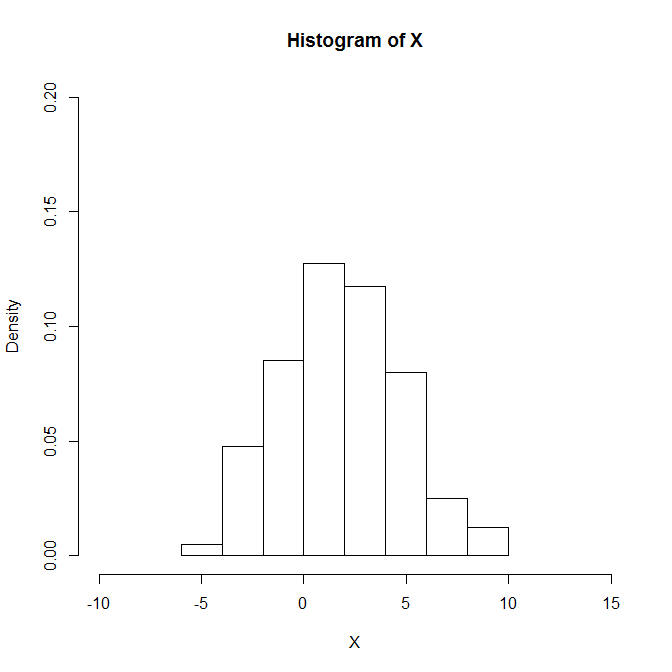
\includegraphics[width=7cm]{hist.png}
\end{center}
As a candidate distribution, for example, consider $N(6, 2)$, which is shown by a blue curve in the next figure:
\begin{center}
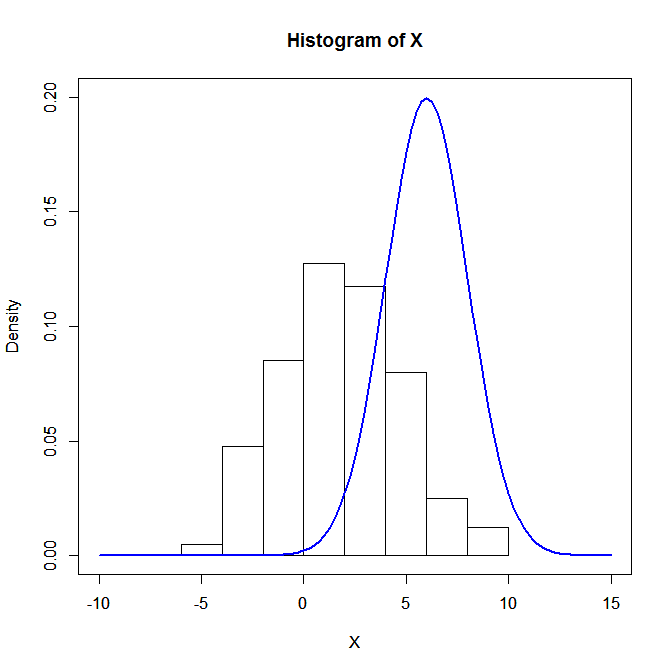
\includegraphics[width=7cm]{hist2.png}
\end{center}
If $N(6, 2)$ is the true distribution of $X$, the values in the neighborhood of $6$ would be most likely observable.
In other words, it is less likely that our data are generated from $N(6, 2)$.
The probability distribution that generates our data with highest likelihood is the one that best fits the histogram:
\begin{center}
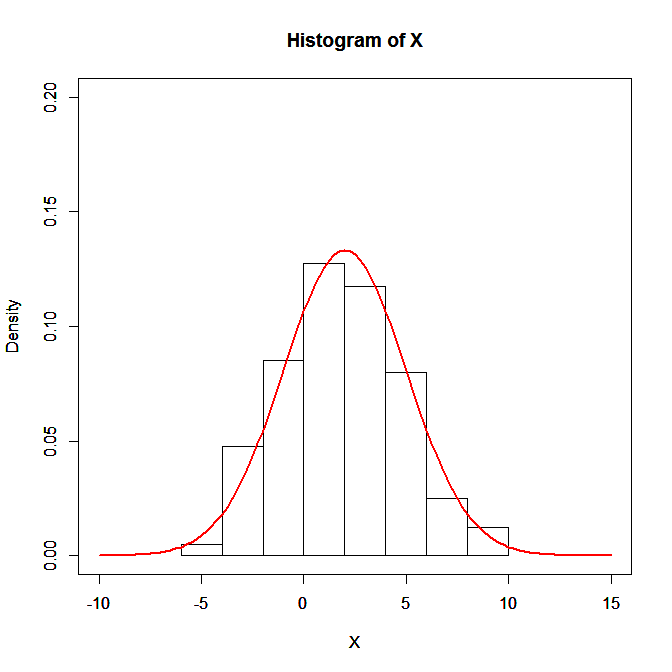
\includegraphics[width=7cm]{hist3.png}
\end{center}
The red curve in the above figure is the normal distribution with its mean and variance being equal to the sample average (1.85) and sample variance (8.55) of $X$, respectively.
Indeed, as stated below, the sample average and sample variance are the \textbf{maximum likelihood estimators\index{maximum likelihood estimator}} (MLE) of $\E X$ and $\Var(X)$, respectively.

\begin{example}[Normal random variable]\label{ex:normal}\upshape
Suppose that we have a set of observations $\{X_1, \ldots, X_n\}$ of size $n$, which are known to be IID normal $N(\mu_0, \sigma_0^2)$, but $\mu_0$ and $\sigma_0^2$ are unknown.
The joint density of the data can be written as
\[
	\text{Joint density of $\{X_1, \ldots, X_n\}$} = \prod_{i=1}^n f_X(X_i)
\] 
by the IID assumption, where $f_X(x) = \frac{1}{\sqrt{2 \pi \sigma_0^2}}\exp\left(-\frac{(x - \mu_0)^2}{2 \sigma_0^2}\right)$.
Since $\mu_0$ and $\sigma_0^2$ are unknown, we consider their candidate values $\mu$ and $\sigma^2$, respectively, and let
\[
	L_n(\theta) \equiv \prod_{i=1}^n f_X(X_i; \mu, \sigma^2),
\]
where $\theta = (\mu, \sigma^2)$, and $f_X(x; \mu, \sigma^2) = \frac{1}{\sqrt{2 \pi \sigma^2}}\exp\left(-\frac{(x - \mu)^2}{2 \sigma^2}\right)$.
The function $L_n(\theta)$ is the joint density of the data under $\theta$, which is called the \textbf{likelihood function\index{lieklihood function}}.
The likelihood function is a function of the parameter $\theta$ such that it coincides with the true joint density when evaluated at $\theta = \theta_0$.
The MLE for $\theta_0$ is defined as the maximizer of the ``log'' of the likelihood, the so-called \textbf{log-likelihood function\index{log-likelihood function}}; that is,
\begin{align}\label{eq:mle-normal}
\begin{split}
	\hat{\theta}^{mle}_n 
		& \equiv \argmax_{\theta} \log L_n(\theta) \\
		& = \argmax_{(\mu, \sigma^2)} \sum_{i=1}^n \log f_X(X_i; \mu, \sigma^2)\\
		& = \argmax_{(\mu, \sigma^2)} \sum_{i=1}^n \left[ - \frac{1}{2}\log \sigma^2 - \frac{(X_i - \mu)^2}{2 \sigma^2}\right] = \argmin_{(\mu, \sigma^2)}  \left[ \frac{n}{2}\log \sigma^2 + \frac{\sum_{i=1}^n (X_i - \mu)^2}{2 \sigma^2}\right].
\end{split}
\end{align}
A theoretical reason for maximizing the log-likelihood function, rather than maximizing the likelihood function itself, will be described later.\footnote{
	An intuitive reason for this is that, without taking the log, the product of the likelihood (probability) tends to zero as $n$ increases.
	}

From the last line of \eqref{eq:mle-normal}, we can see that the MLE $\hat{\mu}^{mle}_n$ of $\mu_0$ can be obtained independently by solving the problem $\min_\mu \sum_{i=1}^n (X_i - \mu)^2$, whose solution is clearly $ \hat{\mu}^{mle}_n = \bar X_n$, where $\bar X_n = \frac{1}{n}\sum_{i=1}^n X_i$.
Hence, the sample average of $X$ is the MLE of $\mu_0$.
For the MLE $\hat{\sigma}^{2, mle}_n$ of $\sigma^2_0$, by the first-order condition it satisfies that
\begin{align*}
	0 = \frac{n}{\hat{\sigma}^{2, mle}_n} - \frac{\sum_{i=1}^n (X_i - \bar X_n)^2}{ \left[\hat{\sigma}^{2, mle}_n \right]^2 },
\end{align*}
which further implies that
\begin{align*}
 \frac{\sum_{i=1}^n (X_i - \bar X_n)^2}{ \hat{\sigma}^{2, mle}_n  } = n \;\; \Rightarrow \;\; \hat{\sigma}^{2, mle}_n = \frac{1}{n} \sum_{i=1}^n (X_i - \bar X_n)^2.
\end{align*}
Thus, the MLE of $\sigma_0^2$ is the sample variance of $X$.
It should be noted that the MLE variance estimator is not an unbiased variance estimator.\footnote{
	As is well known, an unbiased variance estimator is obtained by $\hat{\Var}_n(X) = \frac{1}{n-1}\sum_{i=1}^n (X_i - \bar X_n)^2$.
	}

\end{example}

\begin{example}[Linear regression]\upshape
	We consider the following linear regression model with normally distributed error term:
	\begin{align*}
	& Y_i = X_i^\top \beta_0 + \eps_i, \;\; i = 1, \ldots, n \\
	& \eps_i \sim N(0, \sigma_0^2)
	\end{align*}
	Note that the second line of the above is equivalent to $Y_i - X_i^\top \beta_0 \sim N(0, \sigma_0^2)$.
	Thus, the conditional density of $Y_i$ given $X_i$ can be characterized by
	\[
	Y_i | X_i \sim N(X_i^\top \beta_0, \sigma_0^2).
	\]
	
	Denote the marginal density of $X_i$ as $f_X(\cdot)$, and let $\phi(\cdot ; \mu, \sigma^2)$ be the normal density function with mean $\mu$ and variance $\sigma^2$.
	Then, the joint density of $(Y_i, X_i)$ can be written as
	\[
	f_{Y,X}(Y_i, X_i) = \phi(Y_i ; X_i^\top \beta_0, \sigma_0^2) \cdot f_X(X_i).
	\]
	If the data are IID, the joint density of our data is
	\[
	\text{Joint density of }\{(Y_i, X_i): 1 \le i \le n\} = \prod_{i = 1}^n \phi(Y_i ; X_i^\top \beta_0, \sigma_0^2) \cdot f_X(X_i).
	\]
	Thus, letting $L_n(\theta) \equiv \prod_{i = 1}^n \phi(Y_i ; X_i^\top \beta, \sigma^2) \cdot f_X(X_i)$ be the likelihood function with $\theta = (\beta, \sigma^2)$,  the log-likelihood function is given by
	\begin{align*}
	\log L_n(\theta) = \sum_{i = 1}^n \log \phi(Y_i ; X_i ^\top \beta, \sigma^2) + \sum_{i=1}^n \log f_X(X_i).
	\end{align*}
	Since the second term on the right-hand side is irrelevant to the unknown parameters, the MLE for $\theta_0 = (\beta_0, \sigma_0^2)$ can be obtained by maximizing only the first term:
	\begin{align*}
	\hat \theta_n^{mle} 
	& \equiv \argmax_\theta \log L_n(\theta) \\
	& = \argmax_{(\beta, \sigma^2)} \left[ \sum_{i = 1}^n \log \phi(Y_i ; X_i ^\top \beta, \sigma^2)  \right] =  \argmin_{(\beta, \sigma^2)} \left[ \frac{n}{2}\log \sigma^2 + \frac{\sum_{i=1}^n (Y_i - X_i ^\top \beta)^2}{2 \sigma^2}\right],
	\end{align*}
	where the last equality follows from the same argument as in \eqref{eq:mle-normal}.
	Further, by the similar arguments in Example \ref{ex:normal}, it is easy to see that the MLE $\hat \beta_n^{mle}$ coincides with the OLS estimator and that the MLE $\hat \sigma_n^{2, mle}$ is obtained as the sample variance of the OLS residuals.
\end{example}

\begin{example}[Flipping an uneven coin]\label{ex:coin}\upshape
Suppose that we have a possibly uneven coin such that the probability of heads is unknown and may not be equal to 0.5. 
Let $X$ be a dummy variable defined by
\begin{align*}
&X = 1 \text{ for ``head",}\\
&X = 0 \text{ for ``tail".}
\end{align*}
We use $p_0$ to denote the coin's true probability of heads: $\E X = p_0$. 
Suppose that we have a set of coin-flipping data $\{X_1, \ldots , X_n \}$ of $n$ independent trials.
A natural estimator of $p_0$ is the sample average, i.e., the sample proportion of heads: $\bar{X}_n = \frac{1}{n}\sum_{i = 1}^n X_i$.
In fact, the sample average $\bar{X}_n$ is the least-squares estimator for $p_0$.
To see this, let
\[
	\hat p_n^{ls} \equiv \argmin_{p} \frac{1}{n}\sum_{i=1}^n (X_i - p)^2.
\]
The first-order condition of the minimization problem gives
\begin{align*}
	- \frac{2}{n} \sum_{i = 1}^n (X_i - \hat p_n^{ls}) = 0 \;\; 
	& \Rightarrow \;\; \frac{1}{n}\sum_{i = 1}^n X_i  -  \hat p_n^{ls} = 0 \\
	& \Rightarrow \;\; \hat p_n^{ls} = \bar{X}_n.
\end{align*}

As shown below, $\bar{X}_n$ is also an MLE for $p_0$.
The probability distribution of $X$ is
\[
	\Pr(X = 1) = p_0, \;\; \Pr(X = 0) = 1- p_0
\]
This type of probability distribution is called the \textbf{Bernoulli distribution\index{Bernoulli distribution}}.
By the independence, the joint probability of $\{X_1, \ldots , X_n\}$ is equal to
\[
	\text{Joint probability of $\{X_1, \ldots, X_n\}$} = \prod_{i = 1}^n  p_0^{X_i} (1 - p_0)^{1-X_i}.
\]
Then, the likelihood function is given by $L_n(p) \equiv \prod_{i = 1}^n  p^{X_i} (1 - p)^{1-X_i}$, and the MLE is defined as
\begin{align*}
	\hat{p}^{mle}_n 
	& \equiv \argmax_{p \in (0,1)} \log L_n(p) \\
	& = \argmax_{p \in (0,1)} \sum_{i =1}^n\left\{ X_i\log p + (1 - X_i)\log( 1-p)\right\}.
\end{align*}
The first-order condition for the above maximization implies that 
\begin{align*}
	0
	& = \sum_{i=1}^n\left\{ \frac{X_i}{\hat{p}^{mle}_n} - \frac{1 - X_i}{1 - \hat{p}^{mle}_n} \right\}\\
	%& = \sum_{i=1}^n\left\{ \frac{X_i\cdot (1 - \hat{p}^{mle}_n) - (1 - X_i)\cdot  \hat{p}^{mle}_n}{\hat{p}^{mle}_n \cdot (1 - \hat{p}^{mle}_n)} \right\}  \\	
	& = \sum_{i=1}^n\left\{ \frac{X_i - \hat{p}^{mle}_n}{\hat{p}^{mle}_n \cdot (1 - \hat{p}^{mle}_n)} \right\}.
\end{align*}
Therefore, $\hat{p}_n^{mle}$ must satisfy
\begin{align*}
\sum_{i=1}^n (X_i - \hat{p}_n^{mle}) = 0
& \Rightarrow \hat{p}_n^{mle} = \bar{X}_n.
\end{align*}
\end{example}
\bigskip

We generalize the above discussion.
Suppose we have a set of IID observations $\{X_1, \ldots, X_n\}$ of sample size $n$.
Here, $X$ may be a scalar or a vector.
For continuous (resp. discrete) $X$, let $p(x ; \theta_0)$ be the population density (resp. probability) function of $X$, where $\theta_0$ is the vector of unknown parameters to be estimated.
The functional form of $p(x ; \theta_0)$ is known up to $\theta_0$; that is, $\theta_0$ is the only unknown component.\footnote{
	If the model specification of $p$ is incorrect, then the resulting MLE is not consistent for $\theta_0$.
	Note that, for example in the case of linear regression models, we may use a least-squares method to consistently estimate the parameters even when $p$ is partly unknown.
	In this sense, in general, maximum likelihood methods require more restrictive assumptions than the other types of estimators.
	}
Then, the \textbf{likelihood function\index{likelihood function}} is defined as
\[
	L_n(\theta) \equiv \prod_{i = 1}^n p(X_i; \theta),
\]
and the \textbf{log-likelihood function\index{log-likelihood function}} is
\[
	\ell_n(\theta) \equiv \log L_n(\theta) = \sum_{i = 1}^n \log p(X_i; \theta).
\]
The \textbf{maximum likelihood estimator\index{maximum likelihood estimator}} (MLE) of $\theta_0$ is defined as the maximizer of the log-likelihood function $\ell_n(\theta)$: 
\[
	\hat \theta_n^{mle} \equiv \argmax_{\theta}\ell_n(\theta),
\]
or numerically equivalently,
\begin{align*}
	\hat \theta_n^{mle} 
	& \equiv \argmax_{\theta} \frac{1}{n} \ell_n(\theta) \\ 
	& = \argmax_{\theta} \frac{1}{n} \sum_{i = 1}^n \log p(X_i; \theta).
\end{align*}
Dividing the objective function by $n$ is for technical convenience in deriving the asymptotic properties of MLE.\footnote{
	As $n$ increases to infinity, $\ell_n(\theta)$ may also diverge to infinity since it is a summation of $n$ non-zero terms.
	However, by dividing it by $n$, under standard conditions, we can have $\frac{1}{n} \ell_n(\theta) \overset{p}{\to} \E[\log p(X_i; \theta)]$ for all $\theta$ by the ``uniform" law of large numbers.\label{foot:UWLLN}
	}

\begin{framed}
\begin{exercise}\upshape
	Suppose that we have $n$ IID observations $\{X_1, \ldots, X_n\}$ drawn from a Poisson distribution with parameter $\lambda_0$; i.e.,
	\[
		\Pr(X = k) = \frac{\lambda_0^k \exp(-\lambda_0)}{k !}.
	\]
	Find the MLE of $\lambda_0$.
\end{exercise}
\begin{exercise}\label{ex:maxuni}\upshape
	Suppose that we have $n$ IID observations $\{X_1, \ldots, X_n\}$ drawn from $\text{Uniform}[0, \alpha_0]$.
	Show that the MLE of $\alpha_0$ is given by 
	\[
	\hat \alpha_n^{mle} = \max\{X_1, \ldots, X_n\}. 
	\] 
\end{exercise}
\end{framed}

\subsection{Kullback-Leibler divergence}

Let $p(x; \theta_1)$ and $p(x; \theta_2)$ be two density (or probability) functions such that $p(x; \theta_1) = p(x; \theta_2)$ for all $x$ if and only if $\theta_1 = \theta_2$.
The following quantity is called the \textbf{Kullback-Leibler divergence\index{Kullback-Leibler divergence}}  (KL divergence) between $p(x; \theta_1)$ and $p(x; \theta_2)$:\footnote{
	Note that the KL divergence is not symmetric: $K\left( p(X; \theta_1) \| p(X; \theta_2) \right) \neq K\left( p(X; \theta_2) \| p(X; \theta_1) \right)$, in general.
	In addition, it does not satisfy the triangle inequality.
	Thus, KL divergence is not a distance function. 
	}
\renewcommand{\arraystretch}{1.5}
\begin{align*}
	K\left( p(X; \theta_1) \| p(X; \theta_2) \right)
	& \equiv \E_{\theta_1}\left[\log \frac{p(X; \theta_1)}{p(X; \theta_2)} \right]\\
	& = \left\{ \begin{array}{ll}
		\int \left[\log \frac{p(x; \theta_1)}{p(x; \theta_2)} \right] p(x; \theta_1) \mrm{d}x & \text{ if $X$ is continuous } \\
		\sum_{x \in \{x_1, \ldots , x_k \}} \left[\log \frac{p(x; \theta_1)}{p(x; \theta_2)} \right] p(x; \theta_1) & \text{ if $X$ is discrete with its support $\{x_1, \ldots, x_k\}$}
	\end{array} \right.
\end{align*}
\renewcommand{\arraystretch}{1}
where $\E_{\theta}[\; \cdot \;]$ denotes the expectation under $p(x; \theta)$ (note that $\E[\; \cdot \;] \equiv \E_{\theta_0}[\; \cdot \; ]$, where $\theta_0$ is the true value of $\theta$).
It is straightforward to see that 
\[
	K\left( p(X; \theta_1) \| p(X; \theta_2) \right) = 0
\]
if $\theta_1 = \theta_2$ since $\log 1 = 0$.
Moreover, it holds that for any $\theta_1 \neq \theta_2$, 
\[
	K\left( p(X; \theta_1) \| p(X; \theta_2) \right) > 0.
\]
Formally, we have the following result.
\begin{theorem}\label{thm:KL}
	For any density (or probability) functions $p(x; \theta_1)$ and $p(x; \theta_2)$ such that $p(x; \theta_1) = p(x; \theta_2)$ for all $x$ if and only if $\theta_1 = \theta_2$, it holds that $K(p(x; \theta_1) \| p(x; \theta_2)) \geq 0$.
	The equality holds if and only if $\theta_1 = \theta_2$.
\end{theorem}

\begin{proof}
	We only prove the case when $p(x; \theta)$ is a density function.
	First, note that
	\begin{align*}
		K(p(x; \theta_1) \| p(x; \theta_2))  
		& = \E_{\theta_1}\left[\log \frac{p(X; \theta_1)}{p(X; \theta_2)} \right] \\
		& = \E_{\theta_1}\left[- \log \frac{p(X; \theta_2)}{p(X; \theta_1)} \right].
	\end{align*}
	Then, since $-\log(\cdot)$ is a convex function, by Jensen's inequality \ref{lem:Jensen},
	\begin{align*}
	K(p(x; \theta_1) \| p(x; \theta_2))  
	& \geq -\log \E_{\theta_1}\left[ \frac{p(X; \theta_2)}{p(X; \theta_1)} \right]\\
	& = - \log \int \frac{p(x; \theta_2)}{p(x; \theta_1)}  p(x; \theta_1) \mrm{d}x\\
	& = - \log \int p(x; \theta_2) \mrm{d}x \\
	& = - \log 1 = 0.
	\end{align*}
	This proves the first argument.
	For the second argument, The ``if"-part is trivial.
	To prove the ``only if"-part, note that, if a function $\varphi(\cdot)$ is strictly convex, $\E[\varphi(X)] = \varphi(\E[X])$ occurs only when $X = \E[X]$ (i.e., when $X$ is a constant).
	 Since $- \log(\cdot)$ is a strictly convex function, $K(p(x; \theta_1) \| p(x; \theta_2)) = 0$ holds only when
	 \begin{align*}
	 	\frac{p(X; \theta_2)}{p(X; \theta_1)} 
	 	& =  \E_{\theta_1}\left[ \frac{p(X; \theta_2)}{p(X; \theta_1)} \right]\\
	 	& = \int \frac{p(x; \theta_2)}{p(x; \theta_1)}  p(x; \theta_1) \mrm{d}x\\
	 	& = \int p(x; \theta_2) \mrm{d}x = 1.
	 \end{align*}
	 This implies the desired result.
\end{proof}

\subsection{MLE minimizes the KL divergence}\label{subsec:MLEconsistency}

From Theorem \ref{thm:KL}, for the true parameter $\theta_0$, we can obtain the following trivial equality:
\begin{align*}
	\theta_0 = \argmin_\theta K( p(X; \theta_0) \| p(X; \theta) ).
\end{align*}
 Note that
\begin{align*}
	K( p(X; \theta_0) \| p(X; \theta) )
	&= \E\left[\log \frac{p(X; \theta_0)}{p(X; \theta)} \right]\\
	&= \E[\log p(X; \theta_0)] - \E[\log p(X; \theta) ].
\end{align*}
Since the first term on the right-hand side is irrelevant to $\theta$, it further holds that
\begin{align}\label{eq:pop-mle}
	\theta_0 = \argmax_\theta \E[\log p(X; \theta) ],
\end{align}
implying that the true parameter $\theta_0$ is the maximizer of the population log-likelihood function.
Thus, maximizing the population log-likelihood is equivalent to minimize the KL divergence.

Here, by the law of large numbers, we can expect that
\[
	\frac{1}{n}\sum_{i=1}^n \log p(X_i; \theta) \overset{p}{\to}  \E[\log p(X; \theta) ],
\]
for all $\theta$ (see also Footnote \ref{foot:UWLLN}).
Since $\hat{\theta}_n^{mle} = \argmax_{\theta}\frac{1}{n}\sum_{i=1}^n \log p(X_i; \theta)$, in view of \eqref{eq:pop-mle}, it holds that  $\hat{\theta}_n^{mle} \overset{p}{\to} \theta_0$.
For more precise discussion, see, for example, \cite{newey1994large}.
\begin{center}
	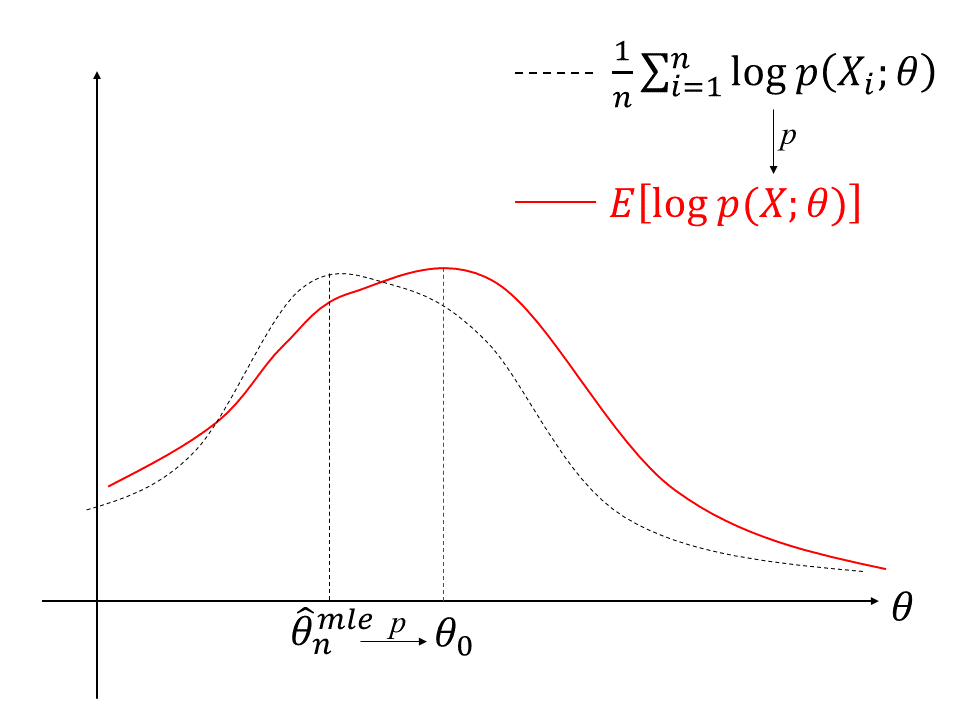
\includegraphics[width=10cm]{mle.png}
\end{center}

\section{Cramer-Rao lower bound}\label{sec:CRLB}
Now, we introduce two important concepts.
The \textbf{score function\index{score function}} (or simply score) is the partial derivative of the log-likelihood $\log p(x; \theta)$ with respect to $\theta$, which we denote by $s(x; \theta)$.
The variance covariance matrix of the score under $p(x; \theta)$ is called the \textbf{Fisher information matrix\index{Fisher infromation matrix}}, which we denote by $I(\theta)$.
Observe that the expectation of the score function (under $p(x; \theta)$) is always zero:
\begin{align}\label{eq:scorezero}
\begin{split}
	\E_\theta[s(X; \theta)]
	& = \int \left\{\frac{\partial}{\partial \theta}\log p(x; \theta)\right\} p(x; \theta) \mrm{d}x \\
	& =  \int \frac{\frac{\partial}{\partial \theta} p(x; \theta)}{p(x; \theta)}p(x; \theta) \mrm{d}x \\
	& = \int \frac{\partial}{\partial \theta} p(x; \theta)  \mrm{d}x \\
	& = \frac{\partial}{\partial \theta} \underbrace{\int p(x; \theta) \mrm{d}x}_{=1} = \mbf{0},
\end{split}
\end{align}
and, therefore
\begin{align*}
	I(\theta) 
	& \equiv \Cov_{\theta}\left[ s(X; \theta) \right] \\
	& = \E_\theta \left[ ( s(X; \theta) - \E_\theta s(X; \theta) ) ( s(X; \theta) - \E_\theta s(X; \theta) )^\top \right] \\
	& = \E_\theta\left[ s(X; \theta) s(X; \theta)^\top \right].
\end{align*}
\bigskip

When estimating $\theta_0$, we can consider many alternative estimators $\hat \theta_n$'s, including OLS, MLE, etc.
An important criterion for the choice of estimator is the \textbf{efficiency\index{efficiency}}; the more efficient estimator is the one that has the smaller variance.
Surprisingly or not, under certain regularity conditions --	see the appendix of this chapter, the inverse of the Fisher information matrix $[I(\theta_0)]^{-1}$ gives the ``lower bound'', known as \textbf{Cramer-Rao lower bound\index{Cramer-Rao lower bound}}, of the covariance matrix for all possible estimators of $\theta_0$; that is, for any ``regular" estimator $\hat \theta_n$ of $\theta_0$,
\begin{align}\label{eq:CRLB}
	\Cov\left(\sqrt{n}(\hat \theta_n - \theta_0)\right) \ge [I(\theta_0)]^{-1}.
\end{align}
Here, for any square matrices $A$ and $B$ of the same size, $A \ge B$ means that $A - B$ is positive-semidefinite.
As described below, the MLE $\hat \theta_n^{mle}$ generally attains this lower bound; that is, \eqref{eq:CRLB} holds with equality.
In other words, whenever the MLE is available, it is the most efficient estimator we can use in the class of regular estimators.
An example of ``irregular'' estimator will be provided in the appendix of this chapter.
\bigskip

We can relatively easily check \eqref{eq:CRLB} if we restrict our attention to the class of unbiased estimators.
Suppose that the data $\{X_1, \ldots , X_n\}$ are IID with density function $p(x; \theta_0)$, where $\theta_0$ is a scalar true parameter for simplicity, and that we have an \textbf{unbiased estimator\index{unbiased estimator}} $\hat \theta_n$ such that
\begin{align}\label{eq:unbiased}
	\E_\theta[\hat \theta_n] - \theta = 0
\end{align}
for any $\theta$.
Note that the above expectation is taken with respect to the data $\{X_1, \ldots , X_n\}$ since any estimator is a function of the data sample; thus, we may write $\hat \theta_n = \theta_n(X_1, \ldots , X_n)$.
\bigskip

\textbf{Proof of \eqref{eq:CRLB} for unbiased estimators.} \quad Since \eqref{eq:unbiased} holds for all $\theta$, differentiating both sides of \eqref{eq:unbiased} with respect to $\theta$, we obtain
\begin{align*}
	0 = \frac{\partial }{\partial \theta}\E_\theta[\hat \theta_n - \theta]
	& = \frac{\partial}{\partial \theta} \int [\theta_n(x_1, \ldots , x_n) - \theta] \prod_{i=1}^n p(x_i; \theta) \mrm{d}x_1 \cdots  \mrm{d}x_n\\
	& = \int [\theta_n(x_1, \ldots , x_n) - \theta] \frac{\partial}{\partial \theta} \prod_{i=1}^n p(x_i; \theta) \mrm{d}x_1 \cdots  \mrm{d}x_n - 1\\
	& = \int [\theta_n(x_1, \ldots , x_n) - \theta]  \left\{ \frac{\partial}{\partial \theta} \log\left( \prod_{i=1}^n p(x_i; \theta) \right) \right\} \prod_{i=1}^n p(x_i; \theta) \mrm{d}x_1 \cdots  \mrm{d}x_n - 1 \\
	& = \int [\theta_n(x_1, \ldots , x_n) - \theta]  \left\{\frac{\partial}{\partial \theta}\sum_{i=1}^n  \log p(x_i; \theta) \right\}\prod_{i=1}^n p(x_i; \theta) \mrm{d}x_1 \cdots  \mrm{d}x_n - 1 \\
	& = \int [\theta_n(x_1, \ldots , x_n) - \theta]  \sum_{i=1}^n s(x_i; \theta) \prod_{i=1}^n p(x_i; \theta) \mrm{d}x_1 \cdots  \mrm{d}x_n - 1\\
	& = \E_\theta\left[ (\hat \theta_n- \theta)  \sum_{i=1}^n s(X_i; \theta)  \right] - 1.
\end{align*}
Recall that $\E_\theta[\hat \theta_n- \theta] = 0$ and $\E_\theta\left[ s(X_i; \theta)  \right] = 0$ by \eqref{eq:scorezero}.
Then, by Cauchy-Schwarz inequality \ref{lem:CS} and the IID assumption, we have
\begin{align*}
	1 
	& \le \left| \E_\theta\left[ \sqrt{n}(\hat \theta_n- \theta) \cdot \frac{1}{\sqrt{n}}  \sum_{i=1}^n s(X_i; \theta)  \right] \right|\\
	& \le \Var_\theta\left( \sqrt{n}(\hat \theta_n- \theta) \right) \Var_\theta\left(\frac{1}{\sqrt{n}}\sum_{i=1}^n s(X_i; \theta) \right)\\
	& = \Var_\theta\left(\sqrt{n}(\hat \theta_n- \theta) \right) I(\theta),
\end{align*}
and, thus,
\[
	\Var_\theta\left(\sqrt{n}(\hat \theta_n- \theta) \right) \ge \frac{1}{I(\theta)}.
\]
$\blacksquare$

\section{Asymptotic properties}
Suppose that we have a consistent MLE $\hat \theta_n^{mle}$ of $\theta_0$.
By the first-order condition, the MLE $\hat \theta_n^{mle}$ satisfies that
\[
	\frac{1}{n}\sum_{i = 1}^n s(X_i; \hat \theta_n^{mle}) = \mbf{0}.
\]
Applying the mean-value expansion to $s(X_i; \hat \theta_n^{mle}) $ around $\theta_0$, we have
\[
	\mbf{0} = \frac{1}{n}\sum_{i = 1}^n s(X_i; \theta_0) + \frac{1}{n}\sum_{i=1}^n H(X_i; \bar \theta_n) (\hat \theta_n^{mle} - \theta_0),
\]
where $H(X_i; \theta) \equiv \partial s(X_i; \theta)/(\partial \theta^\top)$, or equivalently, $H(X_i; \theta) \equiv \partial^2 \log p(X_i; \theta)/(\partial \theta \partial \theta^\top)$, i.e., the Hessian matrix of $\log p(X_i; \theta)$, and $\bar \theta_n \in [\hat \theta_n^{mle}, \theta_0]$.
Then, if $\frac{1}{n}\sum_{i=1}^n H(X_i; \bar \theta_n) $ is nonsingular, we obtain
\begin{align}\label{eq:taylor}
	\sqrt{n}(\hat \theta_n^{mle} - \theta_0) = -\left[\frac{1}{n}\sum_{i=1}^n H(X_i; \bar \theta_n) \right]^{-1}\frac{1}{\sqrt{n}}\sum_{i = 1}^n s(X_i; \theta_0).
\end{align}
As shown in Section \ref{sec:CRLB}, we have $\E[s(X; \theta_0)] = 0$ and $\Cov[s(X; \theta_0)] = I(\theta_0)$.
Since $X_i$'s are IID, so are $s(X_i; \theta_0)$'s.
Then, we can apply CLT to $\frac{1}{\sqrt{n}}\sum_{i = 1}^n s(X_i; \theta_0)$ to obtain
\[
	\frac{1}{\sqrt{n}}\sum_{i = 1}^n s(X_i; \theta_0) \overset{d}{\to} \mbf{N}(\mbf{0},  I(\theta_0)).
\]
Further, note that $\hat \theta_n^{mle}$ is a consistent estimator of $\theta_0$ and so is $\bar{\theta}_n$ clearly by its definition.
Then, we have $\frac{1}{n}\sum_{i=1}^n H(X_i; \bar \theta_n) \overset{p}{\to} \E[H(X; \theta_0)]$ by WLLN, assuming that $H(x; \theta)$ is continuous at $\theta_0$.
Finally, combining these results and applying Slutsky's theorem \ref{lem:slutsky} give the following result:
\[
	\sqrt{n}(\hat \theta_n^{mle} - \theta_0) \overset{d}{\to} \mbf{N}\left( \mbf{0}, \E[H(X; \theta_0)]^{-1} I(\theta_0) \E[H(X; \theta_0)]^{-1} \right).
\]
From this result, one might think that the MLE is not necessarily the most efficient estimation method.
However, that is not the case; that is, the MLE is always the most efficient because of the following fact:
\begin{align}\label{eq:infoeq}
	I(\theta_0) = - \E[H(X; \theta_0)].
\end{align}
This equality is known as the \textbf{information matrix equality\index{information matrix equality}}.
\bigskip

\textbf{Proof of \eqref{eq:infoeq}.} \quad Since \eqref{eq:scorezero} holds for any $\theta$, differentiating both sides of \eqref{eq:scorezero} with respect to $\theta$, we have
\begin{align*}
	\mbf{0} = \frac{\partial }{\partial \theta^\top} \E_\theta[s(X; \theta)] 
	& = \frac{\partial}{\partial \theta^\top}\int s(x; \theta) p(x; \theta) \mrm{d}x \\
	& = \int H(x; \theta) p(x; \theta) \mrm{d}x + \int s(x; \theta) \frac{\frac{\partial}{\partial \theta^\top} p(x; \theta)}{p(x; \theta)} p(x; \theta) \mrm{d}x \\
	& = \int H(x; \theta) p(x; \theta) \mrm{d}x + \int s(x; \theta) s(x; \theta)^\top p(x; \theta) \mrm{d}x.
\end{align*} 
The last line implies that $-\E_\theta[H(X; \theta)] = \E_\theta[s(X; \theta) s(X; \theta)^\top]$.
Finally, the result follows from the definition of $I(\theta)$. $\; \blacksquare$

Therefore, thanks to the information matrix equality, the asymptotic distribution of the MLE can be simply written in two ways as
\begin{align*}
	& \sqrt{n}(\hat \theta_n^{mle} - \theta_0) \overset{d}{\to} \mbf{N}\left( \mbf{0}, -\E[H(X; \theta_0)]^{-1}  \right) \\
	& \sqrt{n}(\hat \theta_n^{mle} - \theta_0) \overset{d}{\to} \mbf{N}\left( \mbf{0}, [I(\theta_0)]^{-1}  \right).
\end{align*}

\section{An application: Binary response models}\label{sec:binary}
As an important application of the maximum likelihood method, we consider estimating binary response models.
Let $D$ be a binary outcome variable defined by
\[
	D = \mbf{1}\{X^\top\beta_0 \ge \eps\},
\]
where $X$ is a vector of explanatory variables, $\eps$ is an unobserved error term, and $\beta_0$ is the vector of parameters to be estimated.

First of all, note that for any constant $c > 0$, it holds that  $D = \mbf{1}\{X^\top(c\beta_0) \ge \eta\}$, where $\eta$ is a new error term defined as $\eta = c\eps$.
Thus, when the distribution of $\eps$ is fully unrestricted, $\beta_0$ cannot be ``identified" without some scale normalization (more formal discussion will be provided in Chapter \ref{chap:identification}). 
To overcome this issue, we typically impose a scale restriction on $\eps$ by assuming that $\eps$ is distributed as either the standard normal or standard logistic with location 0 and scale 1.
The resulting model based on the former assumption is called the \textbf{probit model\index{probit model}} and the one based on the latter is called the \textbf{logit model\index{logit model}}.

Then, under appropriate scale normalization, we can estimate $\beta_0$ by the maximum likelihood method in the following manner.
Observe that the conditional probability of $D = 1$ given $X$ is equal to
\[
	\Pr(D = 1 \mid X) = \Pr( \eps \le X^\top\beta_0 \mid X) = F(X^\top\beta_0),
\]
where $F(\cdot)$ is the distribution function of $\eps$, which is a known function.
Suppose that we have the data of $n$ IID observations $\{(D_i, X_i): 1 \le i \le n\}$.
Then, similarly as in Example \ref{ex:coin}, the (conditional) likelihood function for the data is given by
\[
	L_n(\beta) \equiv \prod_{i=1}^n F(X_i^\top\beta)^{D_i} (1 -  F(X_i^\top\beta))^{1 - D_i},
\] 
and thus the MLE of $\beta_0$ is defined as
\begin{align*}
	\hat \beta_n^{mle} 
	& \equiv \argmax_\beta \log L_n(\beta) \\
	& = \argmax_\beta \sum_{i =1}^n\left\{ D_i \cdot \log F(X_i^\top \beta) + (1 - D_i) \cdot \log(1 -  F(X_i^\top\beta)) \right\}.
\end{align*}
Next, we derive the Fisher information matrix.
To this end, we need to calculate the score function, which is the derivative of  $D \log F(X^\top \beta) + (1 - D) \log(1 -  F(X^\top\beta)$ with respect to $\beta$:
\begin{align*}
	s(X; \beta) 
	& = X \frac{D \cdot f(X^\top \beta)}{F(X^\top \beta)} - X \frac{(1 - D) \cdot f(X^\top \beta)}{1 - F(X^\top \beta)}\\
	& = X \frac{(D - F(X^\top \beta))f(X^\top \beta)}{F(X^\top \beta) \cdot (1 -  F(X^\top\beta)) },
\end{align*}
where $f(\cdot)$ is the density function of $\eps$.
Thus, noting that 
\[
	\E[(D - F(X^\top\beta_0))^2|X] = F(X^\top \beta_0) (1 - F(X^\top \beta_0)),
\]
the information matrix $I(\beta_0)$ is obtained by
\begin{align*}
	I(\beta_0)
	& = \E\left[ s(X; \beta_0) s(X; \beta_0)^\top \right] \\ 
	& = \E\left[ XX^\top  \frac{(D - F(X^\top \beta_0))^2 [f(X^\top \beta_0)]^2}{[F(X^\top \beta_0) \cdot (1 -  F(X^\top\beta_0))]^2 }\right] \\
	& = \E\left[ XX^\top  \frac{[f(X^\top \beta_0)]^2}{F(X^\top \beta_0) \cdot (1 -  F(X^\top\beta_0)) }\right] 
\end{align*}
by LIE.
Hence, we have
\[
	\sqrt{n}(\hat \beta_n^{mle} - \beta_0) \overset{d}{\to} \mbf{N}\left( \mbf{0}, \E\left[ XX^\top  \frac{[f(X^\top \beta_0)]^2}{F(X^\top \beta_0) \cdot (1 -  F(X^\top\beta_0)) }\right]^{-1}  \right).
\]

It is also straightforward to confirm the information matrix equality.
By the chain rule, the Hessian $H(X; \beta_0)$ can be written as
\begin{align*}
	H(X; \beta_0) 
	& = \partial s(X; \beta_0)/ \partial \beta^\top \\
	& = - XX^\top \frac{[f(X^\top \beta_0)]^2}{F(X^\top \beta_0) \cdot (1 -  F(X^\top\beta_0)) } + X (D - F(X^\top \beta_0)) \cdot \frac{\partial}{\partial \beta^\top} \left[ \frac{f(X^\top \beta_0)}{F(X^\top \beta_0) \cdot (1 -  F(X^\top\beta_0)) }\right].
\end{align*}
By LIE, we can see that the second term on the right-hand side will be zero after taking the expectation.
Thus, we have $-\E[H(X; \beta_0) ] = I(\beta_0)$, as desired.

\begin{framed}
\begin{exercise}\upshape
	Consider an ordered choice model with three ordered outcomes:
	\begin{align*}
	Y^* 
	= X^\top\beta_0 + \eps, \qquad D = 1 \iff  \qquad\:  Y^* & \le c_1 \\
	D = 2  \iff c_1 < Y^* & \le c_2 \\
	D = 3  \iff c_2 < Y^* &,
	\end{align*}
	where $Y^*$ is an unobservable latent variable, and $\theta_0 = (\beta_0, c_1, c_2)$ is the set of unknown parameters to be estimated.
	Suppose that we have an IID sample $\{(D_i, X_i): 1 \le i \le n\}$.
	The error term $\eps$ is assumed to be independent of $X$ and has a known distribution function $F$.
	Derive the log-likelihood function for this model and define the MLE $\hat \theta_n^{mle}$ of $\theta_0$.
\end{exercise}
\end{framed}

\section{Likelihood ratio test}\label{sec:LRT}
Partition the estimation parameters as $\theta_0 = (\theta_{01}, \theta_{02})$, where $\theta_{01}$ is a $q_1 \times 1$ vector, and $\theta_{02}$ is a $q_2 \times 1$ vector.
Suppose that we would like to test the following null hypothesis:
\[
	\mbb{H}_0: \theta_{02} = \theta_{02}^*.
\]
The alternative hypothesis is that at least one element of $\theta_{02}$ is not equal to the corresponding element of $\theta_{02}^*$, which is written as
\[
	\mbb{H}_1: \theta_{02} \neq \theta_{02}^*.
\]
By the maximum likelihood principle, it holds that 
\[
	\ell_n(\hat \theta_{n1}^{mle}, \hat \theta_{n2}^{mle}) \ge \ell_n(\tilde \theta_{n1}^{mle}, \theta_{02}^*),
\]
where $(\hat \theta_{n1}^{mle}, \hat \theta_{n2}^{mle})$ is the MLE of $(\theta_{01}, \theta_{02})$ under $\mbb{H}_1$, and $\tilde \theta_{n1}^{mle}$ is the ``restricted'' MLE of $\theta_{01}$ under $\mbb{H}_0$; namely, $\tilde \theta_{n1}^{mle} = \argmax_{\theta_1} \ell_n(\theta_1, \theta_{02}^*)$.
If $\mbb{H}_1$ is true, then we can expect that the former maximized log-likelihood will be significantly larger than the latter.
Thus, we can use the the difference of these log-likelihoods as a valid test statistic for $\mbb{H}_0$.
Let
\begin{align*}
	T_n 
	& \equiv 2\left(\ell_n(\hat \theta_{n1}, \hat \theta_{n2}) - \ell_n(\tilde \theta_{n1}, \theta_{02}^*) \right)\\
	& = 2 \log \frac{L_n( \hat \theta_{n1}, \hat \theta_{n2})}{L_n( \tilde \theta_{n1}, \theta_{02}^*)},
\end{align*}
where the superscript ``\textit{mle}'' is omitted for simplicity.
This test statistic is called the \textbf{likelihood ratio statistic\index{likelihood ratio statistic}}. 
Then, under certain regularity conditions, we can show that 
\begin{align}\label{eq:LRT}
T_n \overset{d}{\to} \chi^2(q_2)
\end{align}
under $\mbb{H}_0$.
Thus, if the computed $T_n$ is sufficiently large compared with the critical value of $\chi^2(q_2)$, then we can reject $\mbb{H}_0$.
This testing procedure is called the \textbf{likelihood ratio test\index{likelihood ratio test}}.
\bigskip

For a better understanding, it would be useful to provide a sketch of the proof of \eqref{eq:LRT} for a simpler case, where $\theta_0$ is a scaler and the null hypothesis is $\mbb{H}_0: \theta_0 = \theta_0^*$.
In this case, the test statistic is simplified as follows: $T_n \equiv 2\left(\ell_n(\hat \theta_n) - \ell_n(\theta_0^*) \right)$.
By the second order Taylor expansion, we have
\begin{align*}
	\ell_n(\theta_0^*) - \ell_n(\hat \theta_n)
	& =  (\theta_0^* - \hat \theta_n) \cdot \ell_n'(\hat \theta_n) + \frac{1}{2}(\theta_0^* - \hat \theta_n)^2 \cdot \ell_n''(\bar \theta_n)\\
	& = \frac{1}{2}(\theta_0^* - \hat \theta_n)^2 \cdot \ell_n''(\bar \theta_n)
\end{align*}
where $\ell_n'(\hat \theta_n)$ and $\ell_n''(\hat \theta_n)$ are the first and second derivatives of $\ell_n$ evaluated at $\hat \theta_n$, respectively, and $\bar \theta_n \in [\theta_0^*, \hat \theta_n]$.
The second equality holds from the first order condition of the maximum likelihood estimation.
Hence, we can write
\begin{align*}
	T_n 
	& = -(\theta_0^* - \hat \theta_n)^2 \cdot \ell_n''(\bar \theta_n)\\
	& =  (\sqrt{n}(\hat \theta_n - \theta_0^*))^2 \cdot \left( - \frac{1}{n}\ell_n''(\bar \theta_n) \right).
\end{align*}
Observe that under $\mbb{H}_0: \theta_0 = \theta_0^*$, we can have $\sqrt{n}(\hat \theta_n - \theta_0^*) = \sqrt{n}(\hat \theta_n - \theta_0)$, and
\[
	-\frac{1}{n} \ell_n''(\bar \theta_n) = -\frac{1}{n} \sum_{i=1}^n \frac{\partial^2 \log p(X_i, \bar \theta_n)}{\partial \theta \partial \theta} \overset{p}{\to} -\E[H(X; \theta_0^*)] = I(\theta_0).
\]
Since $\sqrt{n}(\hat \theta_n - \theta_0) \overset{d}{\to} N(0, [I(\theta_0)]^{-1})$, 
\begin{align*}
	T_n \approx \Bigg[ \: \underbrace{\frac{\sqrt{n}(\hat \theta_n - \theta_0)}{\sqrt{I(\theta_0)}}}_{\overset{d}{\to} \: N(0,1)} \: \Bigg]^2 \overset{d}{\to} \chi^2(1).
\end{align*}


\paragraph{A numerical simulation with R}
The following code gives the simulated distributions of $T_n$ for the coin-flipping data in Example \ref{ex:coin} with $n = 500$ and $\mbb{H}_0: p = p^*$ for $p^* \in \{0.5, 0.55, 0.6\}$.
Here, the true value of $p$ is set to 0.5.

We first define the log-likelihood function:
\begin{lstlisting}[basicstyle=\ttfamily\footnotesize, frame=single]
 LL <- function(p){ 
 
	LogP <- X*log(p) + (1 - X)*log(1 - p)
	ell  <- sum(LogP)
	return(ell)

	}
\end{lstlisting}
Next, we calculate the test statistic $T_n$ for each $\mbb{H}_0$ for 5000 replicated datasets:
\begin{lstlisting}[basicstyle=\ttfamily\footnotesize, frame=single]
 nrep <- 5000
 T0   <- numeric(nrep)
 T1   <- numeric(nrep)
 T2   <- numeric(nrep)

 for(i in 1:nrep){

	X   <- rbinom(500, 1, 0.5)  # flipping an even coin 500 times
	mle <- mean(X)              # MLE = sample average

	T0[i] <- 2*(LL(mle) - LL(0.5 ))
	T1[i] <- 2*(LL(mle) - LL(0.55))
	T2[i] <- 2*(LL(mle) - LL(0.6 ))

	}
\end{lstlisting}
Finally, plot the densities of the calculated $T_n$'s:
\begin{lstlisting}[basicstyle=\ttfamily\scriptsize, frame=single]
 xlm <- c(0,20)
 ylm <- c(0,1)
 xlb <- "T_n"
 ylb <- "Density"
 
 plot(density(T0), xlim = xlm, ylim = ylm, col = 2, main = "", xlab = xlb, ylab = ylb)
 par(new = T)
 plot(density(T1), xlim = xlm, ylim = ylm, col = 3, main = "", xlab = xlb, ylab = ylb)
 par(new = T)
 plot(density(T2), xlim = xlm, ylim = ylm, col = 4, main = "", xlab = xlb, ylab = ylb)
 par(new = T)
 curve(dchisq(x,1), xlim = xlm, ylim = ylm, lwd = 2, lty = 2, main = "", xlab = xlb, ylab = ylb)
 legend(
	"topright",
	c("p = 0.5", "p = 0.55", "p = 0.6", "ChiSq(1)"), 
	lwd = c(1,1,1,2),
	lty = c(1,1,1,2),
	col = c(2,3,4,1)
	) 
\end{lstlisting}
\begin{center}
	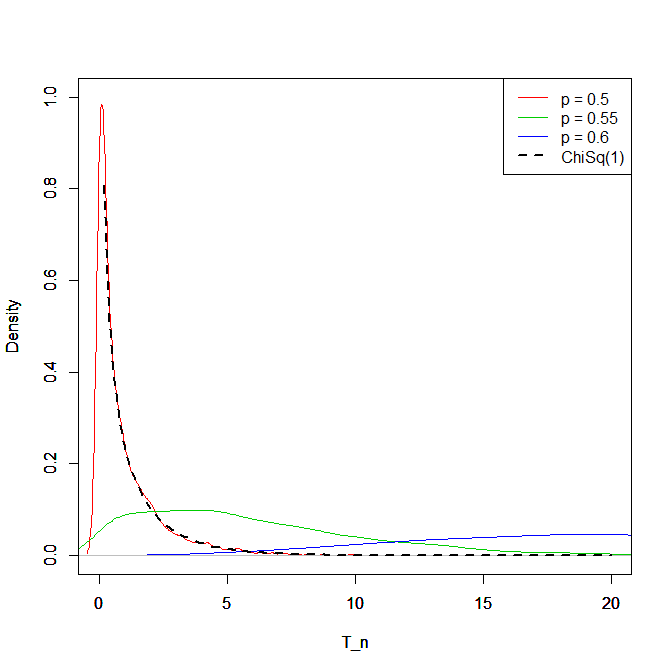
\includegraphics[width=10cm]{LRTsim.png}
\end{center}

\section{Akaike's Information Criterion}

When the number of regressors is large and only some of them are meaningful, including all of them in the model may cause an \textbf{overfitting\index{overfitting}} problem.
That is, using too many explanatory variables results in a model that adapts to the data too well, and shows poor performance in out-of-sample predictions.
In an extreme case, when the number of regressors is equal to the sample size $n$, it is possible to achieve a ``perfect'' fit to the data with zero residuals, but such a model has no predictive power.

In order to avoid the overfitting problem, we need to select the regressors that should be included in the model using some criterion.
Note that the log-likelihood is not a valid variable selection criterion since it monotonically increases in the number of included regressors; model selection based on the log-likelihood value always results in the largest model.
A ``good'' model should be defined as a model whose likelihood function well approximates the ``true'' data distribution, rather than the empirical distribution of the observed data.
\bigskip

Here, let $f_X(x)$ be the true density function of $X$.
The parameterized density $p(x; \theta_0)$ may or may not be equal to $f_X(x)$ (if they are not same, $\theta_0$ is interpreted as a ``pseudo'' true parameter).
Let $\hat \theta_n = \theta_n(X_1, \ldots, X_n)$ be the MLE from our model and $p(x; \hat \theta_n)$ be the estimated likelihood function.
Then, taking the sampling error involved in the estimate of $\hat \theta_n$ into account, we may conclude that our modelling is optimal if the following statistic is sufficiently small:
\begin{align*}
		\E_{data} K( f_X(X) \| p(X; \hat \theta_n) )
		& = \E_{data} \E_X\left[ \log \frac{f_X(X)}{p(X; \hat \theta_n)} \right] \quad \left(=\int\int \log \frac{f(x)}{p(x; \theta_n(x_1, \ldots, x_n))} f_X(x)\mrm{d}x \prod_{i=1}^n f(x_i) \mrm{d}x_i \right)\\
		& = \E_X[\log f_X(X)] - \E_{data} \E_X[\log p(X; \hat \theta_n)],
\end{align*}
which is the expected KL divergence between the true data distribution and the estimated distribution.
Since the first term is independent of the model selection, minimizing the KL divergence over the whole model space is equal to maximizing $\E_{data} \E_X[\log p(X; \hat \theta_n)]$.

By using the second order Taylor expansion around $\theta_0$, we have
\[
	\log p(X; \hat \theta_n) \approx \log p(X; \theta_0) + s(X; \theta_0)^\top (\hat \theta_n - \theta_0) + R_n(X; \hat \theta_n ),
\]
where $R_n(X; \hat \theta_n ) \equiv \frac{1}{2}(\hat \theta_n - \theta_0)^\top H(X; \theta_0) (\hat \theta_n - \theta_0)$.
Further, by \eqref{eq:scorezero},
\begin{align}\label{eq:aic1}
	\E_X[\log p(X; \hat \theta_n)] - \E_X[\log p(X; \theta_0)] \approx \E_X[R_n(X; \hat \theta_n )].
\end{align}
Also, letting $\bar s_n(\theta_0) \equiv \frac{1}{n}\sum_{i = 1}^n s(X_i; \theta_0)$, observe that by \eqref{eq:taylor} and the information matrix equality \eqref{eq:infoeq},
\begin{align}\label{eq:aic2}
\begin{split}
	 \frac{1}{n}\sum_{i = 1}^n \log p(X_i; \hat \theta_n) - \E_X[\log p(X; \theta_0)] 
	& \approx \frac{1}{n}\sum_{i = 1}^n \left(\log p(X_i; \hat \theta_n) - \log p(X_i; \theta_0) \right) \\
	& \approx \bar s_n(\theta_0)^\top (\hat \theta_n - \theta_0) + \frac{1}{n}\sum_{i=1}^nR_n(X_i; \hat \theta_n ) \\
	& \approx -\bar s_n(\theta_0)^\top \underbrace{\left[\frac{1}{n}\sum_{i=1}^n H(X_i; \bar \theta_n) \right]^{-1}}_{\overset{p}{\to}\: -[I(\theta_0)]^{-1}}\bar s_n(\theta_0) +  \E_X[R_n(X; \hat \theta_n )].
\end{split}
\end{align}
Combining \eqref{eq:aic1} and \eqref{eq:aic2} yields
\[
	\frac{1}{n}\sum_{i = 1}^n \log p(X_i; \hat \theta_n) - \E_X[\log p(X; \hat \theta_n)] \approx \bar s_n(\theta_0)^\top [I(\theta_0)]^{-1}\bar s_n(\theta_0).
\]
Then, under the IID assumption,
\begin{align*}
\begin{split}
	\E_{data} \left[\frac{1}{n}\sum_{i = 1}^n \log p(X_i; \hat \theta_n) - \E_X[\log p(X; \hat \theta_n)]\right]
	& \approx \E_{data}\left[\bar s_n(\theta_0)^\top [I(\theta_0)]^{-1}\bar s_n(\theta_0)\right]\\
	& =\text{trace}\left\{ [I(\theta_0)]^{-1}\E_{data}\left[ \bar s_n(\theta_0)\bar s_n(\theta_0)^\top \right] \right\}\\
	& =\text{trace}\Bigg\{ [I(\theta_0)]^{-1}\Bigg(\frac{1}{n}\sum_{i = 1}^n \underbrace{\E_{data}\left[ s(X_i; \theta_0) s(X_i; \theta_0)^\top \right]}_{= \: I(\theta_0)} \Bigg) \Bigg\}/n\\
	& = \frac{\text{trace}\left\{I_{\text{dim}(\theta_0)}\right\}}{n} = \frac{\text{dim}(\theta_0)}{n}.
\end{split}
\end{align*}
Finally, this implies that we can approximate $\E_{data} \E_X[\log p(X; \hat \theta_n)]$ by
\begin{align*}
	\E_{data} \E_X[\log p(X; \hat \theta_n)] 
	& \approx \frac{1}{n}\sum_{i = 1}^n \log p(X_i; \hat \theta_n) - \frac{\text{dim}(\theta_0)}{n}\\
	& = \frac{1}{n} ( \ell_n(\hat \theta_n) - \text{dim}(\theta_0) ) = - \frac{1}{2n} \text{AIC}, 
\end{align*}
where $\text{AIC}$ is defined as
\[
	\text{AIC} \equiv - 2\ell_n(\hat \theta_n) + 2 \text{dim}(\theta_0).
\]
Hence, minimizing the AIC is approximately equivalent to choosing a model which has minimum KL divergence to the true data distribution.
This way of model selection was first proposed in \cite{akaike1973information}, which is known as \textbf{Akaike's Information Criterion\index{Akaike's Information Criterion}}.
\begin{center}
	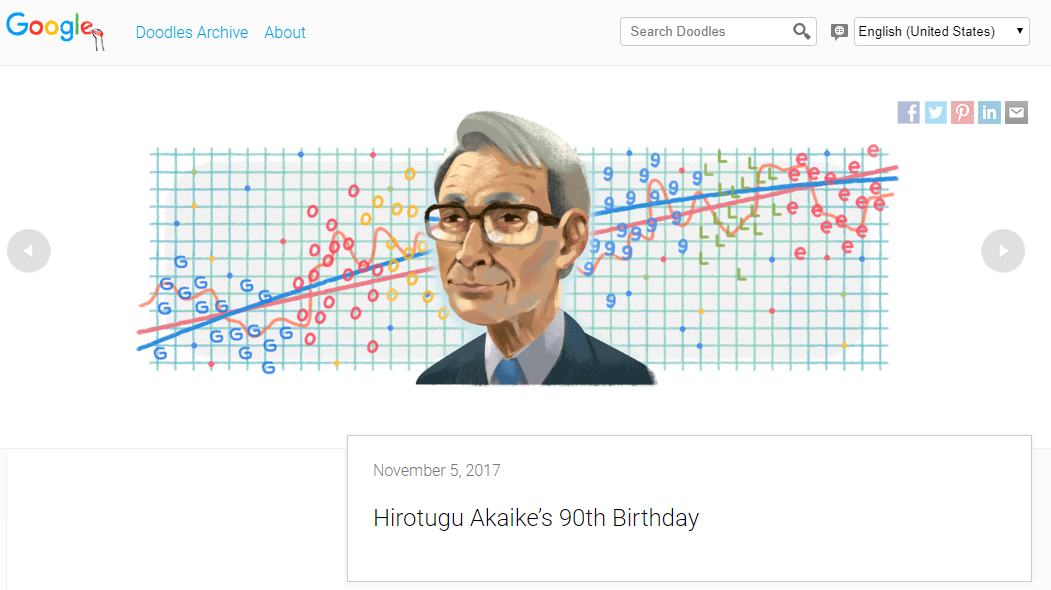
\includegraphics[width=12cm]{akaike.png}
\end{center}
It should be noted that the derivation of the AIC statistic involves a lot of large sample approximations, and it is known that the AIC tends to select a less parsimonious model under finite sample size.
Then, to improve the finite sample model selection performance, a number of modified versions of AIC has been proposed in the literature.

\section*{Appendix: Irregular estimators}

Let $\{X_1, \ldots, X_n\}$ be an IID sample drawn from $N(\mu_0, 1)$.
Then, the MLE for $\mu_0$ is the sample average $\bar X_n$, and we have the asymptotic normality result: $\sqrt{n}(\bar X_n - \mu_0) \overset{d}{\to} N(0, 1)$. 
Note that this argument holds for any given $\mu_0$.

Now, we consider the following estimator:
\begin{align*}
	\hat \mu_n = \begin{cases}
		\bar X_n & \text{if \;\; $|\bar X_n| \ge n^{-1/4}$}\\
		0        & \text{if \;\; $|\bar X_n| < n^{-1/4}$}
	\end{cases}
\end{align*}
This estimator is known as \textbf{Hodge's estimator\index{Hodge's estimator}}.
Namely, Hodge's estimator returns the MLE when $|\bar X_n| \ge n^{-1/4}$ and zero when $|\bar X_n|$ does not exceed $n^{-1/4}$.

To derive the limiting distribution of Hodge's estimator, we first consider the case where $\mu_0 \neq 0$.
Then, since $|\mu_0| - n^{-1/4} > 0$ for sufficiently large $n$, we have
\begin{align*}
	\Pr(\hat \mu_n \neq \bar X_n) 
	& = \Pr(|\mu_0 - (\mu_0 - \bar X_n) | < n^{-1/4}) \\
	& \le \Pr(|\mu_0| - |\mu_0 - \bar X_n| < n^{-1/4}) \\
	& = \Pr(|\mu_0| - n^{-1/4} < |\mu_0 - \bar X_n|) \to 0
\end{align*}
as $n \to \infty$.
This implies that $\hat \mu_n$ has the same limiting distribution as the MLE; that is, $\sqrt{n}(\hat \mu_n - \mu_0) \overset{d}{\to} N(0, 1)$.

Next, consider the case where $\mu_0 = 0$.
In this case, for any $\kappa > 0$,
\begin{align*}
	\Pr\left(\left| \sqrt{n} \hat \mu_n \right| > \kappa \right) 
	& = \Pr\left(\left| \sqrt{n}\hat \mu_n \right| > \kappa, \hat \mu_n = 0\right) + \Pr\left( \left| \sqrt{n} \hat \mu_n \right| > \kappa, \hat \mu_n \neq 0\right) \\
	& = \Pr(\left| \sqrt{n} \hat \mu_n \right| > \kappa, \hat \mu_n \neq 0)  \le \Pr( \hat \mu_n \neq 0). 
\end{align*}
Note that
\begin{align*}
	\Pr( \hat \mu_n \neq 0) 
	& = \Pr(|\bar X_n| \ge n^{-1/4}) \\
	& = \Pr(\sqrt{n}|\bar X_n - \mu_0| \ge n^{1/4}) \to 0
\end{align*}
as $n \to \infty$ since $\sqrt{n}|\bar X_n - \mu_0|$ is asymptotically equivalent to $|N(0,1)|$.
Hence, $\sqrt{n}\hat \mu_n \overset{p}{\to} 0$ and, in view of Lemma \ref{lem:p_to_d}, $\sqrt{n}\hat \mu_n \overset{d}{\to} 0$.
To summarize, the limiting distribution of Hodge's estimator is
\begin{align*}
	\sqrt{n}(\hat \mu_n - \mu_0) \overset{d}{\to} \begin{cases}
		N(0,1) & \text{if \;\; $\mu_0 \neq 0$}\\
		0      & \text{if \;\; $\mu_0 = 0$}.
	\end{cases}
\end{align*}
Although it is tempting to interpret this result as indicating that Hodge's estimator is better than the MLE, Hodge's estimator has a serious drawback.
When $\mu_0$ is away from zero, $\hat \mu_n$ behaves almost like the MLE.
However, as $\mu_0$ gets closer to zero, it differs from the MLE quite often.
To see this, we investigate the performance of $\hat \mu_n$ when $\mu_0 = h/n^{1/4}$ for some $0 < h < 1$.
The data $\{X_1, \ldots, X_n\}$ are drawn from $N(h/n^{1/4}, 1)$ for each $n$.
The asymptotic distribution of the MLE does not change under $\mu_0 = h/n^{1/4}$: $\sqrt{n}(\bar X_n - h/n^{1/4}) \overset{d}{\to} N(0,1)$.
On the other hand,
\begin{align*}
	\Pr(\hat \mu_n = 0)
	& = \Pr(|\bar X_n| < n^{-1/4}) \\
	& = \Pr(- n^{-1/4} < \bar X_n < n^{-1/4}) \\
	& = \Pr \left(- \sqrt{n}(n^{-1/4} + h n^{-1/4}) < \sqrt{n}(\bar X_n - h n^{-1/4}) < \sqrt{n}(n^{-1/4} - h n^{-1/4}) \right) \\
	& = \Pr\left(-n^{1/4}(1 + h) < \sqrt{n}(\bar X_n - h n^{-1/4}) < n^{1/4}(1 - h)\right) \to 1.
\end{align*}
Hence,
\begin{align*}
	\sqrt{n}(\hat \mu_n - h/n^{1/4}) = hn^{1/4} + o_P(1) \to \infty.
\end{align*}
Thus, the MSE of Hodge's estimator $\E [\{\sqrt{n}(\hat \mu_n - \mu_0)\}^2]$ explodes to infinity as $n$ increases when $\mu_0$ is close to zero, whereas $\E[\{\sqrt{n}(\bar X_n - \mu_0)\}^2] = 1$ holds for any $\mu_0$.
Figure \ref{fig:hodge} shows the graphs of the MSE of Hodge's estimator for three different $n$'s.
The R code to create this figure is attached below.
Hodge's estimator ``buys'' its extremely better asymptotic behavior exactly at $\mu_0 = 0$ at the cost of erratic behavior close to zero.

\begin{figure}[h!]
	\begin{center}
		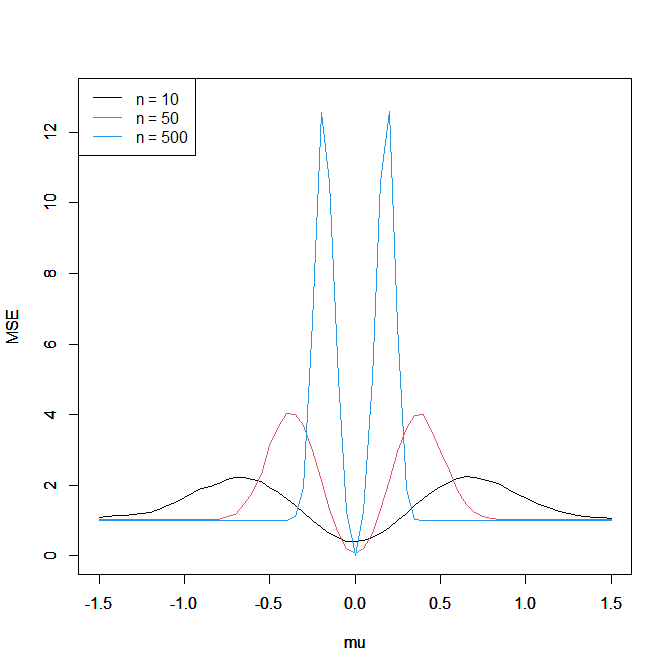
\includegraphics[width = 9cm]{hodge.png}
		\caption{MSE of Hodge's estimator}
		\label{fig:hodge}
	\end{center}
\end{figure}

The above discussion shows that in order to have a meaningful discussion on the efficiency of estimators, we need to rule out pathological estimators such as Hodge's estimator and focus on ``regular'' estimators.
An estimator $\hat \theta_n$ is called \textbf{regular\index{regular estimators}} if a small change in the true parameter $\theta_0$ changes the distribution of the estimator only slightly.
Hodge's estimator is a typical example of ``irregular'' estimators.
Within the class of regular estimators, we can show the optimality of MLE.
For more precise discussion, see, for example, Section 8.5 of \cite{van2000asymptotic}.

\bigskip

\textbf{R code to create Figure \ref{fig:hodge}}

\bigskip

\begin{lstlisting}[basicstyle=\ttfamily\footnotesize, frame=single]
ns  <- c(10, 50, 500)
mus <- seq(-1.5, 1.5, 0.05)

mse <- function(n, mu){

	se <- function(seed){
	   set.seed(seed)
	   X <- rnorm(n, mean = mu, sd = 1)
	   Xbar <- mean(X)
	   H <- 0*(abs(Xbar) < n^{-1/4}) + Xbar*(abs(Xbar) >= n^{-1/4})
	   se <- (sqrt(n)*(H - mu))^2
	   return(se)
	   }

   R <- numeric(2000)
   for(r in 1:2000) R[r] <- se(r)
   return(mean(R))
	
   }
	
result <- matrix(0, length(ns), length(mus))
for(i in 1:length(ns)) for(j in 1:length(mus)) result[i,j] <- mse(ns[i],mus[j])

plot(mus, result[1,], ylim = c(0,13), xlab = "mu", ylab = "MSE", type = "l", col = 1)
par(new = T)
plot(mus, result[2,], ylim = c(0,13), xlab = "mu", ylab = "MSE", type = "l", col = 2)
par(new = T)
plot(mus, result[3,], ylim = c(0,13), xlab = "mu", ylab = "MSE", type = "l", col = 4)
legend("topleft", legend = c("n = 10", "n = 50", "n = 500"), lty = c(1, 1, 1), col = c(1, 2, 4))
\end{lstlisting}


%%%%%%%%%%%%%%%%%%%%%%%%%%%%%%%%%%%%%%%%%%%%%%%%
%%%%%%%%%%%%%%%%%%%%%%%%%%%%%%%%%%%%%%%%%%%%%%%%
%%%%%%%%%%%%%%%%%%%%%%%%%%%%%%%%%%%%%%%%%%%%%%%%

\chapter{Generalized Method of Moments}\label{chap:gmm}
\section{Moment conditions}\label{sec:mom}

Consider the following multiple regression model:
\begin{align*}
	Y = X_1^\top \theta_0 + \eps.
\end{align*}
We assume that the regressor $\underset{d_{x1} \times 1}{X_1}$ is exogenous: $\E [X_1 \eps] = \mbf{0}$, and that $\E[X_1 X_1^\top]$ is nonsingular.
Then, one can estimate $\theta_0$ by the OLS estimator based on the following moment equations:
\begin{align*}
	\underset{d_{x1} \times 1}{\mbf{0}} = \E[X_1 \eps] = \E[X_1 (Y - X_1^\top\theta_0)]  \iff \theta_0 = \E[X_1 X_1^\top]^{-1} \E[X_1 Y].
\end{align*}
Note here that the number of moment equations $\underset{d_{x1} \times 1}{\E[X_1 (Y - X_1^\top \theta_0)] = \mbf{0}}$ available is exactly the same as the number of elements in $\underset{d_{x1} \times 1}{\theta_0}$.
In this case we say that $\theta_0$ is \textbf{just-identified\index{just-identification}}.\footnote{
	It is well-known in linear algebra that when the number of independent linear equations equals the number of unknowns, the system can be uniquely solved.
}

Now suppose that we know that not only $X_1$ but also $\underset{d_{x2} \times 1}{X_2}$ satisfies the same moment equality $\E [X_2 \eps] = \mbf{0}$.\footnote{$X_2$ could be a function of $X_1$; see also footnote \ref{foot:ols_moment} in Chapter \ref{chap:LLN_CLT}.}
For simplicity suppose that $d_{x1} = d_{x2}$.
These additional $d_{x2}$ moment conditions $\underset{d_{x2} \times 1}{\E[X_2 (Y - X_1^\top \theta_0)] = \mbf{0}}$ can be utilized in the estimation of $\theta_0$.
That is, if $\E [X_2X_1^\top]^{-1}$ exists, we can characterize $\theta_0$ alternatively by
\[
	\theta_0 = \E[X_2 X_1^\top]^{-1} \E[X_2 Y].
\]
This situation is called \textbf{over-identification\index{over-identification}}; that is, the number of available moment equations is larger than the number of unknowns.
In other words, we can write down $\theta_0$ as a function of the moments in several different ways. 
\bigskip

The above example is a special case of a more general class of moment restriction models.
Let $g(W; \theta)$ be an $\mbb{R}^J$-valued function, where $\theta$ is a $K \times 1$ vector of parameters, and $W$ is a vector of observable random variables.
We assume that $J \geq K$.
Suppose that the following moment conditions hold:
\begin{align}\label{eq:momcond}
	\E[g(W; \theta_0)] = \underset{J \times 1}{\mbf{0}},
\end{align}
where $\theta_0$ is the true value of $\theta$.
In the above multiple regression model, $g(W; \theta_0)$ corresponds to $(X_1^\top, X_2^\top)^\top (Y - X_1^\top\theta_0)$, and $W$ corresponds to $(Y, X_1, X_2)$; thus, in this case, $J = d_{x1} + d_{x2}$ and $K = d_{x1}$ (note that any two linearly dependent moment conditions are counted as the same moment condition).
If $J = K$, we say that $\theta_0$ is just-identified, and if $J > K$, it is over-identified.

\begin{example}[Linear regression]\label{ex:ols}\upshape
	Consider the following linear regression model with exogenous regressors:
	\[
	Y = X^\top\theta_0 + \eps, \;\; \E[X \eps] = \mbf{0}.
	\]
	Then, setting $g(W; \theta) = X( Y - X^\top\theta)$ gives \eqref{eq:momcond} with $W = (Y,X)$.
\end{example}

\begin{example}[Instrumental variables regression]\label{ex:2sls}\upshape
	Consider the following linear regression model with both endogenous and exogenous regressors:
	\[
	Y = D^\top\alpha_0 + X^\top\beta_0 + \eps, \;\; \E[D \eps] \neq \mbf{0}, \;\; \E[X \eps] = \mbf{0}.
	\]
	Suppose that we have a set of instrumental variables $Z_1$ for $D$, and let $Z = (Z_1^\top, X^\top)^\top$.
	Then, we have $\E [Z \eps] = \mbf{0}$, which gives \eqref{eq:momcond} by setting $g(W; \theta) = Z( Y - D^\top\alpha - X^\top\beta)$ with $\theta_0 = (\alpha_0^\top, \beta_0^\top)^\top$ and $W = (Y,D,X,Z_1)$.
\end{example}

\begin{example}[Probit model 1]\upshape\label{ex:probit}
	Consider the following probit model:
	\[
		D = \mbf{1}\{X^\top\theta_0 \geq \eps\}, \;\; \eps \sim N(0,1).
	\]
	Assuming that $\eps$ is independent of $X$, the conditional expectation of $D$ given $X$ is $\E [D \mid X] = \Phi(X^\top \theta_0)$, where $\Phi$ is the standard normal distribution function.
	Trivially, this implies that
	\[
		\E[D -  \Phi(X^\top \theta_0) \mid X] = 0.
	\]
	This ``conditional" moment restriction implies the ``unconditional" moment restrictions $\E [X (D -  \Phi(X^\top \theta_0))] = \mbf{0}$ by LIE:
	\begin{align*}
	\E [X (D -  \Phi(X^\top \theta_0))] 
	& = \E \left\{ \E[X (D -  \Phi(X^\top \theta_0)) \mid X] \right\} \\
	& = \E \left\{ X \E[ D -  \Phi(X^\top \theta_0) \mid X] \right\} = \E \left( X \times 0 \right) = \mbf{0}.
	\end{align*}
	Hence, setting $g(W; \theta) = X (D -  \Phi(X^\top \theta))$ with $W = (D,X)$, the probit model also fits in the framework of \eqref{eq:momcond}.
\end{example}

\begin{example}[Probit model 2]\label{ex:prob2}\upshape
	There are other moment conditions that can be used to estimate the probit model.
	First, note that the true parameter $\theta_0$  can be characterized as the maximizer of the population log-likelihood function (see Section \ref{subsec:MLEconsistency}):
	\[
		\theta_0 = \argmax_\theta \E\left[ D \cdot \log \Phi(X^\top \theta) + (1 - D) \cdot \log (1 - \Phi(X^\top \theta ) )  \right].
	\]
	The first order condition for this maximization problem is
	\[
		\E\left[ X  \eta(\theta_0) \right] = \mbf{0},
	\]
	where
	\[
		\eta(\theta_0) \equiv \frac{(D - \Phi(X^\top \theta_0)) \cdot \phi(X ^\top \theta_0)}{\Phi(X^\top \theta_0) \cdot (1 - \Phi(X^\top \theta_0) )},
	\]
	and $\phi$ is the standard normal density function.
	Thus, the score function $X  \eta(\theta)$ serves as $g(W; \theta)$
	
	Here, the term $\eta(\theta_0)$ is referred to as the ``generalized residual" for the probit model; this is the conditional expectation of $-\eps$ given $(D, X)$.
	Namely, using the formula for the expectation of a truncated random variable (see Appendix \ref{sec:truncate}) and the fact  that $-e\phi(e) = \phi'(e)$, we have
	\begin{align*}
		\E[-\eps \mid X, D = 1] = \E[-\eps \mid X, X^\top\theta_0 \geq \eps] 
		& = -\frac{\int_{-\infty}^{X^\top\theta_0} e \phi(e) \mrm{d}e}{\Phi(X^\top\theta_0)} \\
		& =  \frac{ \int_{-\infty}^{X^\top\theta_0} \phi'(e) \mrm{d}e}{\Phi(X^\top\theta_0)} = \underbrace{\frac{ \phi(X^\top \theta_0)}{\Phi(X^\top\theta_0)}}_{= \: \eta(\theta_0)|_{D = 1}}\\
		\E[-\eps \mid X, D = 0] = \E[-\eps \mid X, X^\top\theta_0 < \eps] 
		& = - \frac{\int_{X^\top\theta_0}^\infty e \phi(e) \mrm{d}e}{1 - \Phi(X^\top\theta_0)} \\
		& = \frac{ \int_{X^\top\theta_0}^\infty \phi'(e) \mrm{d}e}{1- \Phi(X^\top\theta_0)} = \underbrace{-\frac{ \phi(X^\top \theta_0)}{1- \Phi(X^\top\theta_0)}}_{= \: \eta(\theta_0)|_{D = 0}}.
	\end{align*}
\end{example}

\section{GMM procedure}
When the data of sample size $n$ are available, the sample analogue of $\E [g(W; \theta)]$ can be obtained by
\[
	\bar{g}_n(\theta) \equiv \frac{1}{n}\sum_{i = 1}^n g(W_i; \theta).
\]
Then, by the law of large numbers, we can expect that $\bar{g}_n(\theta_0) \approx \mbf{0}$ for sufficiently large $n$.
This implies that one can consider estimating $\theta_0$ by solving
\begin{align}\label{eq:mm_estimator}
	\bar{g}_n(\theta) = \mbf{0}
\end{align}
with respect to $\theta$.
This type of estimator is called the \textbf{method of moments\index{method of moments}} estimator.
The method of moments estimator has a unique solution when $J = K$ (i.e., just-identification) under appropriate rank conditions.
However, in general $J > K$, the parameter value that exactly satisfies \eqref{eq:mm_estimator} may not exist.

The idea of the \textbf{generalized method of moments\index{generalized method of moments}} (GMM) is to obtain an estimator of $\theta_0$ by finding a $\theta$ that makes $\bar{g}_n(\theta)$ as close to zero as possible. 
To do this, let $\Omega_n$ be a $J \times J$ positive definite symmetric ``weight" matrix.
Then, the GMM estimator of $\theta_0$ is defined by
\begin{align}\label{eq:gmm}
	\hat{\theta}_n^{gmm} \equiv \argmin_{\theta} \bar{g}_n(\theta)^\top \Omega_n \bar{g}_n(\theta).
\end{align}
Since the objective function in \eqref{eq:gmm} has a quadratic form and $\Omega_n$ is positive definite, it holds that $\bar{g}_n(\theta)^\top \Omega_n \bar{g}_n(\theta) \geq 0$ for any $\theta$.
One can simply choose an identity matrix $I_J$ of dimension $J$ as $\Omega_n$.
In this case, $\hat{\theta}_n^{gmm}$ is defined as the minimizer of $||\bar{g}_n(\theta) ||^2$.
However, as discussed later, the choice of the weight matrix affects the efficiency of the estimator.

\begin{example}[Linear regression (cont.)]\upshape
	Letting $g(W_i; \theta) = X_i( Y_i - X_i^\top\theta)$, we have
	\[
	\bar{g}_n(\theta) = \mbf{X}_n^\top (\mbf{Y}_n - \mbf{X}_n \theta)/n,
	\]
	where $\mbf{X}_n = (X_1, \ldots , X_n)^\top$, and $\mbf{Y}_n = (Y_1, \ldots , Y_n)^\top$.
	Thus, the GMM estimator $\hat\theta_n^{gmm}$ is obtained by
	\begin{align*}
		\hat{\theta}_n^{gmm} = \argmin_{\theta} (\mbf{Y}_n - \mbf{X}_n \theta)^\top \mbf{X}_n \Omega_n \mbf{X}_n^\top (\mbf{Y}_n - \mbf{X}_n \theta).
	\end{align*} 
	Solving the first order condition gives
	\begin{align*}
		- 2\mbf{X}_n^\top \mbf{X}_n \Omega_n \mbf{X}_n^\top (\mbf{Y}_n - \mbf{X}_n \hat\theta_n^{gmm}) = \mbf{0} 
		& \iff \mbf{X}_n^\top \mbf{X}_n \Omega_n \mbf{X}_n^\top (\mbf{Y}_n - \mbf{X}_n \hat\theta_n^{gmm}) = \mbf{0} \\
		& \iff \;\; \hat\theta_n^{gmm} = \left[\mbf{X}_n^\top \mbf{X}_n \Omega_n \mbf{X}_n^\top\mbf{X}_n \right]^{-1} \mbf{X}_n^\top \mbf{X}_n \Omega_n \mbf{X}_n^\top\mbf{Y}_n.
	\end{align*}
	This implies that the OLS estimator is a special case of the GMM estimator in which the weight matrix $\Omega_n$ is chosen as $\Omega_n = (\mbf{X}_n^\top \mbf{X}_n)^{-1}$.
\end{example}

\begin{example}[Instrumental variables regression (cont.)]\upshape
	Let $H = (D^\top, X^\top)^\top$ and $g(W_i; \theta) = Z_i (Y_i - H_i^\top\theta)$.
	Then, we have
	\[
	\bar{g}_n(\theta) = \mbf{Z}_n^\top (\mbf{Y}_n - \mbf{H}_n \theta)/n,
	\]
	where $\mbf{Z}_n = (Z_1, \ldots, Z_n)^\top$, and $\mbf{H}_n = (H_1, \ldots , H_n)^\top$.
	Similarly as above, the GMM estimator $\hat\theta_n^{gmm}$ can be obtained by
	\begin{align*}
		\hat{\theta}_n^{gmm} = \argmin_{\theta} (\mbf{Y}_n - \mbf{H}_n \theta)^\top \mbf{Z}_n \Omega_n \mbf{Z}_n^\top (\mbf{Y}_n - \mbf{H}_n \theta).
	\end{align*}
	By easy calculations,
	\[
	\hat \theta_n^{gmm} = \left[\mbf{H}_n^\top \mbf{Z}_n \Omega_n \mbf{Z}_n^\top\mbf{H}_n \right]^{-1} \mbf{H}_n^\top \mbf{Z}_n \Omega_n \mbf{Z}_n^\top\mbf{Y}_n.
	\]
	Thus, when setting the weight matrix $\Omega_n$ as $\Omega_n = (\mbf{Z}_n^\top \mbf{Z}_n)^{-1}$, we can see that  the GMM estimator coincides with the 2SLS estimator (see \eqref{eq:2slsMat}).
\end{example}

\section{Asymptotic properties}\label{sec:asympGMM}
Let $\Omega \equiv \plim_{n \to \infty} \Omega_n$.
Suppose that the true parameter $\theta_0$ can be characterized as
\[
	\theta_0 = \argmin_\theta \E[g(W; \theta)]^\top \Omega \E[g(W; \theta)].
\]
Then, under some regularity conditions, one can show that the GMM estimator $\hat \theta_n^{gmm}$ is consistent for $\theta_0$ (see, e.g., \cite{newey1994large}).

The asymptotic distribution of $\hat\theta_n^{gmm}$ can be derived as follows.
Hereinafter, we suppress the superscript ``$gmm$'' for notational simplicity.
By the first order condition for the minimization in \eqref{eq:gmm}, it holds that
\[
	\bar{g}'_n(\hat\theta_n)^\top \Omega_n \bar{g}_n(\hat\theta_n) = \underset{K \times 1}{\mbf{0}},
\] 
where $\bar{g}'_n( \theta) = \underset{J \times K}{\partial \bar{g}_n(\theta) / \partial \theta^\top}$.
Applying the mean-value expansion to $\bar{g}_n(\hat\theta_n)$ around $\theta_0$, we have
\[
	\mbf{0} = \bar{g}'_n(\hat\theta_n)^\top \Omega_n \left[\bar{g}_n(\theta_0) +  \bar{g}'_n(\bar{\theta}_n) (\hat\theta_n - \theta_0) \right],
\]
where $\bar{\theta}_n \in [ \hat\theta_n, \theta_0]$.
This implies that
\begin{align*}
	\sqrt{n} (\hat\theta_n - \theta_0) 
	& = -\left[ \bar{g}'_n(\hat\theta_n)^\top \Omega_n \bar{g}'_n(\bar{\theta}_n) \right]^{-1} \bar{g}'_n(\hat\theta_n)^\top \Omega_n (\sqrt{n}\bar{g}_n(\theta_0))  \\
	& = -\left[ \bar{g}'_n(\hat\theta_n)^\top \Omega_n \bar{g}'_n(\bar{\theta}_n) \right]^{-1} \bar{g}'_n(\hat\theta_n)^\top \Omega_n \left[\frac{1}{\sqrt{n}}\sum_{i=1}^n g(W_i; \theta_0)\right].
\end{align*}
Letting $V \equiv \E[g(W; \theta_0)g(W; \theta_0)^\top]$ and assuming that the data are IID, by CLT, we have
\[
	\frac{1}{\sqrt{n}}\sum_{i=1}^n g(W_i; \theta_0) \overset{d}{\to} \mbf{N}(\mbf{0}, V).
\]
In addition, by WLLN, $\bar{g}'_n(\theta_0) \overset{p}{\to} M \equiv  \E[ \partial g(W; \theta_0) / \partial \theta^\top]$.
Note that if $\hat\theta_n$ is a consistent estimator of $\theta_0$, so is $\bar{\theta}_n$ by its definition. 
Thus, by the continuous mapping theorem, we obtain both $\bar{g}'_n(\hat\theta_n) \overset{p}{\to} M$ and $\bar{g}'_n(\bar{\theta}_n) \overset{p}{\to} M$.
Finally, by Slutsky's theorem \ref{lem:slutsky}, we have the asymptotic normality of $\sqrt{n} (\hat\theta_n - \theta_0)$ as follows:
\begin{align}\label{eq:GMMnormal}
\begin{split}
	\sqrt{n} (\hat\theta_n - \theta_0) 
	& \overset{d}{\to} \mbf{N}\left(\mbf{0},  (M^\top \Omega M )^{-1} M^\top \Omega V \Omega M ( M^\top \Omega M )^{-1} \right).
\end{split}
\end{align}

\begin{framed}
\begin{exercise}\upshape
	Consider a linear regression model:
	\[
	Y = X^\top \beta_0 + \eps,
	\]
	where the conditional median of $\eps$ given $X$ is zero: $\text{Med}[\eps \mid X] = 0$.
	Describe how to construct a GMM estimator of $\beta_0$. 
\end{exercise}

\begin{exercise}\upshape
	Consider an endogenous probit model:
	\[
		Y = \mbf{1}\{\beta_0 + D \alpha_0 \ge \eps\}, \;\; \eps \sim N(0,1),
	\]
	where $D$ is potentially dependent on $\eps$.
	Suppose that there is an IV $Z_1$ for $D$ such that it is a determinant of $D$ and is independent of $\eps$. 
	An analyst tries to estimate $\theta_0 = (\beta_0, \alpha_0)^\top$ using GMM with $g(W; \theta) = Z(Y - \Phi(\beta + D \alpha))$ by analogy from Example \ref{ex:probit}, where $Z = (1, Z_1)^\top$, and $W = (Y,D,Z_1)$.
	However, such an estimator is generally inconsistent.
	Explain why.
\end{exercise}
\end{framed}

\section{Two-step optimal GMM}
It can be seen from \eqref{eq:GMMnormal} that the variance of the GMM estimator depends on the choice of the weight matrix $\Omega_n$.
An optimal GMM estimator that achieves the smallest possible asymptotic variance can be obtained by setting $\Omega_n = V_n^{-1}$ such that $\plim_{n \to \infty} \Omega_n = V^{-1}$.
With this weight matrix, the asymptotic covariance matrix in \eqref{eq:GMMnormal} can be simplified to
\[
	(M^\top V^{-1} M )^{-1} M^\top V^{-1} V V^{-1} M ( M^\top V^{-1} M )^{-1} =  (M^\top V^{-1} M )^{-1}.
\]
The optimality of this weight matrix can be easily shown as follows.
For any $\Omega$, observe that
\begin{align}\label{eq:matdiff}
\begin{split}
	&  (M^\top \Omega M )^{-1} M^\top \Omega V \Omega M ( M^\top \Omega M )^{-1}   - (M^\top V^{-1} M )^{-1} \\
	& =  (M^\top \Omega M )^{-1} M^\top \Omega V^{1/2}\left\{ I_J -  V^{-1/2}M ( M^\top V^{-1} M )^{-1} M^\top V^{-1/2} \right\} V^{1/2} \Omega M  (M^\top \Omega M )^{-1} \\
	& =   (M^\top \Omega M )^{-1} M^\top \Omega V^{1/2} \left\{ I_J - P (P^\top P)^{-1} P^\top \right\}  V^{1/2} \Omega M  (M^\top \Omega M )^{-1},
\end{split}
\end{align}
where $I_J$ is an identity matrix of dimension $J$, and $P \equiv V^{-1/2}M$.
Note that the matrix $ I_J - P (P^\top P)^{-1} P^\top$ is idempotent, and thus its eigenvalues are either $0$ or $1$.\footnote{\label{foot:idempotent}
	This can be easily proved.
	Let $A$ be an idempotent matrix such that $AA = A$, and $\lambda$ and $x$ be an eigenvalue of $A$ and its corresponding eigenvector, respectively.
	Then, we have
	\[
	\lambda x = Ax = AAx = A(\lambda x) = \lambda Ax = \lambda^2 x.
	\]
	Since the eigenvector $x$ is a nonzero vector by definition, this is possible only when $\lambda = \lambda^2$, implying that $\lambda \in \{0,1\}$.
	}
Therefore, the left-hand side in \eqref{eq:matdiff} is positive semidefinite, implying the optimality of  $\Omega_n = V_n^{-1}$.

Recall that $V = \Cov[g(W; \theta_0)]$.
Thus, its sample analog $V_n$ can be constructed by
\[
	V_n = \frac{1}{n} \sum_{i = 1}^n g(W_i; \theta_0)g(W_i; \theta_0)^\top.
\]
However, since the true parameter $\theta_0$ is unknown, $V_n$ is also unknown, and the optimal GMM is not feasible.
To estimate $V_n$, we first need to obtain a consistent GMM estimator $\hat\theta_n^{gmm}$ of $\theta_0$ with an arbitrary weighting matrix, such as $\Omega_n = I_J$.
This estimator is consistent but not fully efficient, in general.
Then, we can consistently estimate $V_n$ by
\[
	\hat V_n  = \frac{1}{n} \sum_{i = 1}^n g(W_i; \hat\theta_n^{gmm})g(W_i; \hat\theta_n^{gmm})^\top,
\]
and re-estimate $\theta_0$ by
\[
	\hat\theta_n^{opt} \equiv \argmin_{\theta} \bar{g}_n(\theta)^\top \hat V_n^{-1} \bar{g}_n(\theta).
 \] 
 The estimator $\hat\theta_n^{opt} $ is called the \textbf{two-step optimal GMM estimator\index{two-step optimal GMM estimator}}.
The two-step estimator has the same asymptotic distribution as the infeasible optimal GMM:
\[
	\sqrt{n} (\hat\theta_n^{opt} - \theta_0)  \overset{d}{\to} \mbf{N}\left(\mbf{0},  (M^\top V^{-1} M )^{-1}  \right).
\]

\begin{example}[Probit model 2 (cont.)]\upshape
	Let $g(W; \theta) = X\eta(\theta)$, where the $\eta(\theta)$ is as defined in Example \ref{ex:prob2}.
	Since $g(W; \theta)$ is the score function of the log-likelihood, the matrix $V$ is equal to the Fisher information matrix $I(\theta)$.
	Furthermore, recalling the definition $M \equiv  \E[ \partial g(W; \theta_0) / \partial \theta^\top]$, we can see that $M$ is the expected Hessian matrix of the log-likelihood: $M = \E[H(W; \theta_0)]$.
	Finally, by the information matrix equality \eqref{eq:infoeq}, we have
	\[
	\sqrt{n} (\hat\theta_n^{opt} - \theta_0)  \overset{d}{\to} \mbf{N}\left(\mbf{0}, [I(\theta_0)]^{-1}  \right).
	\]
	Thus, the optimal GMM estimator is asymptotically equivalent to the MLE in this case.
\end{example}

\begin{framed}
\begin{exercise}\upshape
	\begin{enumerate}
	\item Consider the multiple regression models in Example \ref{ex:ols}. 
	Prove that the OLS estimator is equivalent to the optimal GMM estimator under homoskedasticity.
	\item Consider the IV regression models in Example \ref{ex:2sls}.
	Prove that the 2SLS estimator is equivalent to the optimal GMM estimator under homoskedasticity.
	\end{enumerate}
\end{exercise}

\begin{exercise}\upshape
	Consider the following model: $Y = \theta_0 + \varepsilon$ with $\E[\eps] = 0$ and, for a $J \times 1$ vector of random variables $X$, $\E[X \varepsilon] = \mbf{0}$.
	Assuming that IID data $\{(Y_i,X_i): 1 \le i \le n\}$ are available, derive the optimal GMM estimator of $\theta_0$.
\end{exercise}
\end{framed}

\section{Over-identification test}

Suppose that we would like to know the validity of our moment conditions by testing the following hypotheses:
\begin{align*}
	& \mbb{H}_0: \E[g(W; \theta_0)] = \mbf{0}\\
	& \mbb{H}_1: \E[g(W; \theta)] \neq \mbf{0} \;\; \text{for all $\theta$}.
\end{align*}
In the case of just-identification $J = K$, it is possible to find a GMM estimator that exactly solves $\bar g_n(\hat \theta_n^{gmm}) = \mbf{0}$.
Note that such $\hat \theta_n^{gmm}$ may exist even when $\mbb{H}_1$ is true.\footnote{
	For example, consider a linear regression model $Y = X^\top \theta_0 + \eps$, where $X$ is endogenous: $\E[X \eps] \neq \mbf{0}$.
	Set $g(W; \theta) = X(Y - X^\top\theta)$ based on the wrong model assumption of $\E[X \eps] = \mbf{0}$.
	Then, we can find a $\hat \theta_n^{gmm}$ that exactly solves $\bar g_n(\hat \theta_n^{gmm}) = \mbf{0}$ (i.e., the OLS estimator), and this estimator is clearly inconsistent.
	}
Therefore, it is generally impossible to statistically test the validity of the moment conditions in a just-identified model.

Suppose now that $J > K$.
Then, by solving $K$ moment equations, we can set them equal to zero.
If all $J$ moment conditions are actually valid, then the remaining $J-K$ moment conditions should also be close to zero, otherwise they are away from zero.
This implies that in an over-identified model, we can test the validity of $J - K$ over-identifying moment conditions.
Under $\mbb{H}_0$, by CLT, we have
\[
	\sqrt{n} V^{-1/2} \bar g_n (\theta_0) \overset{d}{\to} \mbf{N}(\mbf{0}, I_J).
\]
Hence, $n \bar g_n (\theta_0) V^{-1} \bar g_n (\theta_0)$ has a chi-square limit distribution, and we can test $\mbb{H}_0$ based on this fact.
However note that $\theta_0$ and $V$ are unknown.
Thus, replacing them by their consistent estimators, we can show under regularity conditions that
\begin{align*}
	n \bar{g}_n(\hat\theta_n^{gmm})^\top \hat V_n^{-1} \bar{g}_n(\hat\theta_n^{gmm}) \overset{d}{\to} \chi^2(J - K)
\end{align*}
under $\mbb{H}_0$.
Thus, if the value of $n \bar{g}_n(\hat\theta_n^{gmm})^\top \hat V_n^{-1} \bar{g}_n(\hat\theta_n^{gmm})$ is sufficiently large compared with the critical value of $\chi^2(J - K)$, then we can reject $\mbb{H}_0$.
This testing approach is called \textbf{Hansen's over-identification test\index{over-identification test}} (also referred to as Hansen's $J$ test).
Note that the test statistic of the over-identification test is $n$ times the objective function for the optimal GMM.
Thus, the over-identification test can be easily performed as a by-product of the optimal GMM.

%%%%%%%%%%%%%%%%%%%%%%%%%%%%%%%%%%%%%%%%%%%%%%%%%%%%%%
%%%%%%%%%%%%%%%%%%%%%%%%%%%%%%%%%%%%%%%%%%%%%%%%%%%%%%
%%%%%%%%%%%%%%%%%%%%%%%%%%%%%%%%%%%%%%%%%%%%%%%%%%%%%%

\chapter{Identification}\label{chap:identification}

A minimal requirement for an estimator is consistency, that is, the estimator converges in probability to its true value as the sample size tends to infinity. 
A necessary condition for the existence of consistent estimators for a parameter is that the parameter can be ``identified''.
In econometrics, \textbf{identification\index{identification}} means that the parameter of interest can be ``uniquely'' determined from the observable population data (not from the sample observations).
More intuitively, identification means that if we could obtain infinite observations, the true parameter is knowable as a unique value.
For example, for maximum likelihood estimation of a parameter $\theta_0$, we can say ``$\theta_0$ is identified'' if $\theta_0$ uniquely solves the maximization problem in \eqref{eq:pop-mle}: i.e., $\{\theta : \argmax_\theta \E[\log p(X; \theta)]\}$ is a singleton.
If there is another parameter value, say $\theta_1$, that also maximizes $\E [\log p(X; \theta)]$, we cannot distinguish which of the two is the true value.
In this case, $\theta_0$ is not identified, and it is impossible to construct a consistent estimator for $\theta_0$.

In the following, we discuss the identification problem in econometrics more formally with some examples.
Although there are a number of similar identification concepts in econometrics, all of them eventually ask if the model parameters $\theta_0$ can be recovered from the population observable data.
In this chapter, we mainly follow the definitions and terminology in \cite{hurwicz1950generalization} and \cite{matzkin2013nonparametric}.
\begin{screen}
\begin{center}
	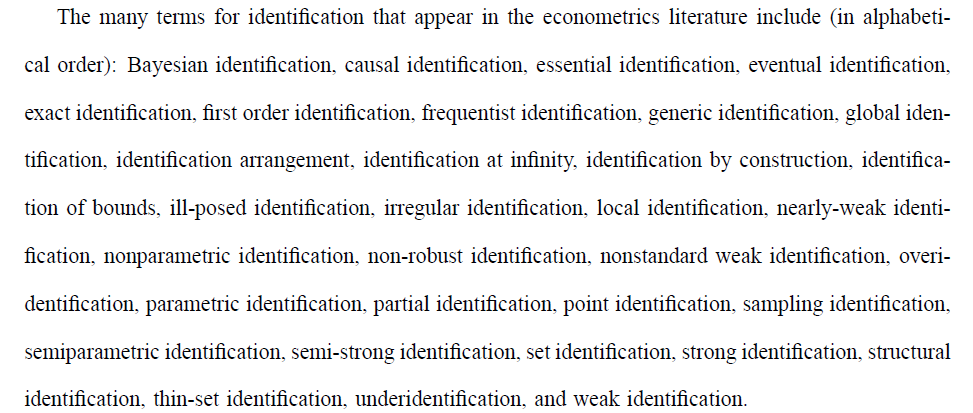
\includegraphics[width=14cm]{identifications.png}

	\footnotesize
	A quote from \cite{lewbel2019identification}
	\normalsize
\end{center}
\end{screen}

\section{A numerical illustration: a heteroskedastic probit model}
Note that the identification problem is indeed crucial in empirical studies.
Even when there seem to be no problems with the data and statistical programming, if identification is not achieved, the resulting estimates are not reliable, or you simply cannot obtain any estimates.

Suppose that a researcher considers estimating the following two heteroskedastic probit models:
\begin{align*}
	\text{Model 1} & \;\; Y = \mbf{1}\{\beta_0 + X \beta_1 \ge \eps\}, \;\; \text{where} \;\; \eps \sim N(0, \sigma^2_1(X)), \;\; \sigma_1(X) = |X\beta_2| \\
	\text{Model 2} & \;\; Y = \mbf{1}\{\beta_0 + X \beta_1 \ge \eps\}, \;\; \text{where} \;\; \eps \sim N(0, \sigma^2_2(X)), \;\; \sigma_2(X) = |(1 + \sqrt{X})\beta_2|.
\end{align*}
Here, we assume that $X$ is one-dimensional and non-negative.
At first glance, both models are quite similar and seem to be valid.
However, as shown numerically below, Model 1 is a faulty model while Model 2 is not.

We generate 1000 observations for each model, where the true parameters $(\beta_0,\beta_1,\beta_2)$ are fixed at $(0,1,1)$ for both models:
\begin{lstlisting}[basicstyle=\ttfamily\footnotesize, frame=single]
# sample size #
 n <- 1000

# true parameters #
 b0 <- 0
 b1 <- 1
 b2 <- 1

# standard deviation functions #
 sd1 <- function(a) abs(X*a)
 sd2 <- function(a) abs((1 + sqrt(X))*a)

# data generation #
 X <- runif(n,0,2) # X ~ Uniform[0,2]
 e1 <- rnorm(n, mean = 0, sd = sd1(b2))
 e2 <- rnorm(n, mean = 0, sd = sd2(b2))
 Y1 <- ifelse(b0 + X*b1 > e1, 1, 0)
 Y2 <- ifelse(b0 + X*b1 > e2, 1, 0)
\end{lstlisting}
The log-likelihood functions are as follows:
\begin{lstlisting}[basicstyle=\ttfamily\footnotesize, frame=single]
 LL1 <- function(p){
	P1 <- pnorm(p[1] + X*p[2], mean = 0, sd = sd1(p[3]))
	P0 <- 1 - P1
	LL <- Y1*log(P1) + (1 - Y1)*log(P0)
	return(-sum(LL))
	}

 LL2 <- function(p){
	P1 <- pnorm(p[1] + X*p[2], mean = 0, sd = sd2(p[3]))
	P0 <- 1 - P1
	LL <- Y2*log(P1) + (1 - Y2)*log(P0)
	return(-sum(LL))
	}
\end{lstlisting}
The obtained MLEs are
\begin{lstlisting}[basicstyle=\ttfamily\footnotesize, frame=single]
	MLE1 <- optim(c(0,1,1), LL1, method = "BFGS")
	>  MLE1
	$par
	[1] -0.01150047  2.94351522  2.85940987
	$convergence
	[1] 0 

	MLE2 <- optim(c(0,1,1), LL2, method = "BFGS")
	>  MLE2
	$par
	[1] -0.0326636  0.9913823  0.9722578
	$convergence
	[1] 0
\end{lstlisting}
Here, \texttt{convergence = 0} means that the optimization has been successfully completed.
However, the estimated parameters for Model 1 are clearly inconsistent with the true values, whereas we can correctly estimate the true parameters in Model 2.

Where does this difference come from?
The only difference between Model 1 and Model 2 is the specification of the standrd deviation function.
In fact, the one used in Model 1 has a serious problem that makes the model unidentifiable, whereas the specification in Model 2 does not have such a problem.

In this example, since we know the values of the true parameters, we can detect that there is something wrong with Model 1.
However, in real situations where we have no prior knowledge about the true model, it is generally a difficult task to determine whether the estimation results are legitimate or not.
One thing we can say for sure is that if the model is not identifiable, the resulting parameter estimates are not consistent.

\section{Definition of identification}

Suppose that a dependent variable $Y$ is uniquely determined by a \textbf{structural equation\index{structural equation}}
\[
	h(Y, X, \eps) = 0,
\]
where $X$ is a vector of observable covariates and $\eps$ is an unobserved error.
We can treat the marginal distribution of $X$ as known.
\cite{hurwicz1950generalization} defines a \textbf{structure} as a system of the structural equation and the distribution of $(X, \eps)$.
More specifically, the pair $S \equiv (h, F_{\eps,X})$ forms a structure, where $F_{\eps,X}$ denotes the joint distribution of $(X, \eps)$.
Then, each $S$ determines the distribution of observable variables $F_{Y,X}$.

Let $F^1_{Y,X}$ and $F^2_{Y,X}$ be the distributions of $(Y, X)$ generated by $S^1 \equiv (h^1, F^1_{\eps,X})$ and $S^2 \equiv (h^2, F^2_{\eps,X})$, respectively.

\begin{definition}
	The structures $S^1$ and $S^2$ are said to be \textbf{observationally equivalent\index{observationally equivalent}} if
	\[
	F^1_{Y,X} = F^2_{Y,X}.
	\]
\end{definition}
In words, when $S^1$ and $S^2$ are observationally equivalent, we cannot distinguish them from observable information alone because they generate the same distribution of observable variables.

A \textbf{model} is defined as a set of such structures with some restrictions on $h$ and $F_{\eps,X}$.
Let us denote the true structure as $S^* \equiv (h^*, F^*_{\eps,X})$.
Denote the set of functions $h$ that satisfy the restrictions that $h^*$ is assumed to satisfy by $H$, and denote the set of distributions $F_{\eps,X}$ that satisfy the restrictions that $F^*_{\eps,X}$ is assumed to satisfy is denoted by $\Gamma$.
Then, we can define a set of ``admissible'' structures as $\mcl{S}_{H,\Gamma} \equiv H \times \Gamma$.

\begin{definition}
	Let $F_{Y,X}$ be the distribution generated by a structure $S \in \mcl{S}_{H,\Gamma}$.
	Then, we say that $S^*$ is identified in $\mcl{S}_{H,\Gamma}$ if
	\[
	F_{Y,X} \neq F^*_{Y,X}
	\]
	for all $S \neq S^*$.
\end{definition} 

Next, consider a \textbf{feature} (or simply a parameter) of a structure, $\theta \equiv \theta(S)$.

\begin{definition}[Point-identification] \label{def:identification}
	The feature $\theta^* \equiv \theta(S^*)$ is point-identified (or simply ``identified'') if for any $S \in \mcl{S}_{H,\Gamma}$ that is observationally equivalent to $S^*$,
	\[
	\theta(S) = \theta(S^*).
	\]
\end{definition}
The above definition says that when the observable variables contain sufficiently rich information to uniquely determine the value of a feature $\theta$ under $\mcl{S}_{H,\Gamma}$, it is identifiable.

\begin{example}[Linear regression models]\upshape
	Consider the following linear regression model:
	\[
		Y = X^\top \beta + \eps,
	\]
	where $Y \in \mbb{R}$, $X \in \mbb{R}^k$, and $\eps \in \mbb{R}$.
	The structural equation is given by
	\[
	 	h(Y, X, \eps) = Y - X^\top \beta - \eps.
	\]
	The set of admissible $h(Y, X, \eps)$'s can be formed simply by 
	\[
		H \equiv \{h : h(Y, X, \eps) = Y -X^\top \beta-\eps,  \beta \in \mbb{R}^k\}.	
	\]
	For an admissible set of distributions $F_{\eps,X}$, for example, consider 
	\[
		\Gamma_1 \equiv \{F_{\eps,X} : \E[\eps \mid X] = 0\}.
	\]
	Then, in the class of models defined by $H \times \Gamma_1$, we can have
	\[
	\E [XY ] = \E[XX^\top] \beta
	\]
	by LIE.
	The above relationship is not sufficient to point-identify $\beta$ because the matrix $\E [XX^\top]$ may not be of full rank.
	That is, there are possibly infinite number of different  $\beta$'s that satisfy the above equality.

	Here, we add one more restriction on $\Gamma_1$.
	Namely, let 
	\[
		\Gamma_2 \equiv \{F_{\eps,X} : \E[\eps \mid X] = 0, \E[XX^\top] \text{ is nonsingular.} \}.
	\]
	Then, for any $S_1, S^* \in H \times \Gamma_2$ that are observationally equivalent, we have
	\begin{align*}
	\beta(S_1) & = \E_1[XX^\top]^{-1} \E_1[XY ] \\
	\beta(S^*) & = \E^*[XX^\top]^{-1} \E^*[XY ],
	\end{align*}
	where $\E_1$ denotes the expectation under $F^1_{Y,X}$ generated by $S_1$, and $\E^*$ denotes the expectation under $F^*_{Y,X}$ generated by $S^*$.
	Since $S_1$ and $S^*$ are observationally equivalent, we have $F^1_{Y,X} = F^*_{Y,X}$, implying that $\E_1[XX^\top]^{-1} = \E^*[XX^\top]^{-1}$ and $\E_1[XY ] = \E^*[XY ]$ hold.
	Thus,  $\beta(S_1) =  \beta(S^*)$ for any $S_1$ that is observationally equivalent to $S^*$, i.e.,  $\beta^* \equiv \beta(S^*)$ is identified.
\end{example}

As shown in the above example, in general, a parameter of interest $\theta^*$ can be identified if we can find a mapping, say $\psi$, such that $\theta^* = \psi(\text{the moments of observed random variables})$ holds.
In this case, we say that the identification is ``constructive''.
Since any observationally equivalent distributions have the same moments of all order, the requirement in Definition \ref{def:identification} is met automatically.
However, it is usually difficult to find such closed-form expressions for $\theta^*$ (of course, the lack of closed-form solution does not imply the failure of identification). 
There are many different, but closely related, notions of identification in the econometrics literature.
For a recent comprehensive survey, see \cite{lewbel2019identification}.

\begin{example}[Binary response models]\upshape
Consider the following binary response model:
\[
	Y = \mbf{1}\{ X^\top \beta \ge \eps\},
\]
where $X \in \mbb{R}^k$, and $\eps \in \mbb{R}$.
The structural equation is
\[
	h(Y, X, \eps) = Y - \mbf{1}\{ X^\top \beta \ge \eps \}.
\]
For simplicity, the following assumption is maintained throughout this part: $\Pr(X^\top \beta = X^\top \beta^*) = 1$
if and only if  $\beta =  \beta^*$ (which is the full-rankness condition in this context).
Further, let
\begin{align*}
	H_1 &
	\equiv \{h : h(Y, X, \eps) = Y - \mbf{1}\{ X^\top \beta \ge \eps\},  \beta \in \mbb{R}^k \}\\
	\Gamma_1 
	& \equiv \{F_{\eps,X} : \eps \text{ is independent of } X, \: \eps \sim N(0, 1)\} \\
	\Gamma_2
	& \equiv \{F_{\eps,X} : \eps \text{ is independent of } X, \: \eps \sim N(0, \sigma^2)\}.
\end{align*}
Note that clearly $\Gamma_1 \subset \Gamma_2$ holds by their definitions.
As it turns out,  $\beta$ can be identified under $H_1 \times \Gamma_1$ but not identified under $H_1 \times \Gamma_2$.
To see this, first focus on the models in $H_1 \times \Gamma_2$.
Then, for any observationally equivalent $S_1, S^* \in H_1 \times \Gamma_2$, we have
\begin{align*}
	\E_1[Y \mid X] 
	& = \Phi \left(\frac{X^\top \beta_1}{\sigma_1} \right) \\
	\E^*[Y \mid X]
	& = \Phi \left(\frac{X^\top \beta^*}{\sigma^*} \right).
\end{align*}
Since $S$ and $S^*$ are observationally equivalent ($F^1_{Y,X} = F^*_{Y,X}$), we have $\E_1[Y \mid X] = \E^*[Y \mid X]$ almost surely (a.s.), which implies
\begin{align}\label{eq:prob_nonident}
	\Phi \left( \frac{X^\top \beta_1}{\sigma_1} \right) = \Phi \left( \frac{X^\top \beta^*}{\sigma^*} \right ) \;\; \text{a.s.}
	\Longrightarrow \Pr\left(\frac{X^\top \beta_1}{\sigma_1} = \frac{X^\top \beta^*}{\sigma^*}\right) = 1
	\Longrightarrow \frac{\beta_1}{\sigma_1} = \frac{\beta^*}{\sigma^*},
\end{align}
where the first $\Longrightarrow$ is by the fact that $\Phi(\cdot)$ is strictly increasing and continuous.
This tells us that the exact value of $\beta^*$ is not identified in $H_1 \times \Gamma_2$; in order to achieve point identification of $\beta^*$, we need to impose an additional restriction on the model which ensures $\sigma_1 = \sigma^*$.
What we can identify within $H_1 \times \Gamma_2$ is only the relative scale of the elements of $\beta^*$.
For example, letting $\beta_{k}^*$ be the $k$-th element of $\beta^*$, it holds by \eqref{eq:prob_nonident} that
\[
	(\beta_{1k}/\sigma_1)/(\beta_{1k'}/\sigma_1) = (\beta_{k}^*/\sigma^*)/(\beta_{k'}^*/\sigma^*) \iff \beta_{1k}/\beta_{1k'} = \beta_{k}^*/\beta_{k'}^*
\]
for all observationally equivalent $S_1$.
In this situation, we say that  $\beta^*$ is identified ``up to scale''.
The above result is intuitively understandable from the fact that for any constant $c > 0$ the following two models
\[
	Y = \mbf{1}\{ X^\top \beta \ge \eps \} \;\; \text{and} \;\; Y = \mbf{1}\{ X^\top(c \beta) \ge c\eps\}
\]
can generate exactly the same distributions for the observable data.
Thus, for identification of  $\beta^*$, we need to introduce some scale normalization restriction.
A convenient way to do so is to assume that $\eps$ is distributed as the standard normal (i.e., probit model).
Then, for models in $H_1 \times \Gamma_1$, since both $\sigma_1$ and $\sigma^*$ are fixed at one, we have $\beta_1 =  \beta^*$ for any $S_1$ observationally equivalent to $S^*$ from \eqref{eq:prob_nonident}, implying that  $\beta^*$ is identifiable.

Other possible identification restrictions are, for example, as follows:
\begin{align*}
	H_2 
	& \equiv \{h : h(Y, X, \eps) = Y - \mbf{1}\{ X^\top \beta \ge \eps\} ,  \beta_1 = 1,  \beta_{-1} \in \mbb{R}^{k-1}\}, \; \text{where }  \beta = ( \beta_1,  \beta^\top_{-1})^\top,\\
	& \footnotesize{\text{(assuming that the first element of  $\beta$ is known to be positive)}} \\
	H_3
	& \equiv \{h : h(Y, X, \eps) = Y - \mbf{1}\{ X^\top \beta \ge \eps \} , \beta \in \mbb{R}^k, || \beta|| = 1\}.
\end{align*}
Then, we can show that $( \beta_{-1}, \sigma^2)$ and $(\beta, \sigma^2)$ are identifiable in $H_2 \times \Gamma_2$ and $H_3 \times \Gamma_2$, respectively.

It would be worth noting that the normality assumption on $\eps$ is in fact not necessary for identification.
With some scale normalization,  $\beta^*$ can be identified even when the distribution function of $\eps$ is completely unknown (see, e.g., \cite{manski1975maximum}).
\end{example}

\begin{framed}
\begin{exercise}\upshape
Suppose that the true system $S^*$ belongs to $\mathcal{S}_{H,\Gamma} \equiv H \times \Gamma$, where
\begin{align*}
	H 
	& \equiv \{h : h(Y,X,\eps) = Y - \phi(X^\top \beta) - \eps, \; \beta \in \mathbb{R}^\text{dim$(X)$}, \; \text{$\phi$ is a known and strictly increasing function}\} \\
	\Gamma
	& \equiv \{F_{\eps, X} : \E[\eps \mid X] = 0, \; \E[XX^\top] \text{ is nonsingular}\}
\end{align*}
Prove that $\beta(S^*)$ is point-identified.
\end{exercise}
\end{framed}

\section{Partial identification}
In the above discussion, we have considered under what conditions a parameter of interest $\theta^* \equiv \theta(S^*)$ can be identified as a unique value.
However, in practice, it is often the case that such identification conditions are quite restrictive and not testable.
Without these conditions, although the exact value of $\theta^*$ may not be identified, if we can still identify $\theta^*_L$ and $\theta^*_U$ such that
\[
	\theta^*_L \le \theta^* \le \theta^*_U,
\]
we can infer the value of $\theta^*$ (for example, if $\theta^*_L$ is positive, we can say at least that $\theta^*$ is positive).
In this situation, we say that $\theta^*$ is ``partially'' identified (or set-identified), and $[\theta^*_L, \theta^*_U]$ is called the identified interval, or more generally, the identified set.
More formal definition is as follows:
\begin{definition}[Partial-identification]
	 The feature $\theta^* \equiv \theta(S^*)$ is \textbf{partially identified\index{partial identification}} if for any $S \in \mcl{S}_{H,\Gamma}$ that is observationally equivalent to $S^*$,
	\[
	\theta(S), \theta(S^*) \in \Theta^*.
	\]
	The set $\Theta^*$ is called the \textbf{identified set\index{identified set}}.
\end{definition}
The identified set $\Theta^*$ is said to be ``informative'' if $\Theta^*$ is a bounded set, and is ``uninformative'' if not.
Note that the identified set is not unique; for an extreme example, $\mbb{R}^{\text{dim}(\theta)}$ is always an (uninformative) identified set for $\theta^*$.
In the literature on partial identification, we are usually interested in finding the smallest (i.e., the most informative) identified set.

\begin{example}[Missing data]\upshape
	Let $Y \in \{0, 1\}$ be a dummy response variable of interest.
	Suppose that $Y$ is not observable for some individuals for some reason, and let $D \in \{0, 1\}$ be a dummy variable indicating the observability of $Y$:
	\begin{align*}
	\left\{ 
	\begin{array}{ll}
	\text{$Y$ is observed} & \text{if $D = 1$}\\
	\text{$Y$ is unobserved} & \text{if $D = 0$}.
	\end{array}\right.
	\end{align*}
	This situation is quite common when the data are collected from a questionnaire survey.
	Suppose that we would like to know the population ratio of $Y = 1$, $\E [Y]$.
	Then, a common practice is to estimate it by estimating instead $\E [Y \mid D = 1]$ using only observable data subset.
	However, in order for the equality $\E [Y] = \E[Y \mid D = 1]$ to hold, we need a strong condition, such as the independence 	between $Y$ and $D$, the so-called \textbf{missing at random\index{missing at random}} assumption.

	Even when $Y$ and $D$ are dependent, in general, we can construct an informative identified interval for $\E [Y]$.
	First, observe that
	\[
		\E[Y] = \E[Y \mid D = 1] \Pr(D = 1) + \E[Y \mid D = 0] \Pr(D = 0).
	\]
	For the terms on the right-hand side, only $\E [Y \mid D = 0]$ is an unknown component.
	Note that we must have $0 \le \E[Y \mid D = 0] \le 1$ since $Y$ is a dummy variable.
	Thus, the following inequalities must hold:
	\[
		\E[Y \mid D = 1] \Pr(D = 1) \le \E[Y] \le \E[Y \mid D = 1] \Pr(D = 1) + \Pr(D = 0).
	\]
	Hence, the identified interval for $\E [Y ]$ is given by
	\[
		\Theta'_{\E[Y]} \equiv \Big[ \E[Y \mid D = 1] \Pr(D = 1), \: \E[Y \mid D = 1] \Pr(D = 1) + \Pr(D = 0) \Big] .
	\]

	\begin{center}
		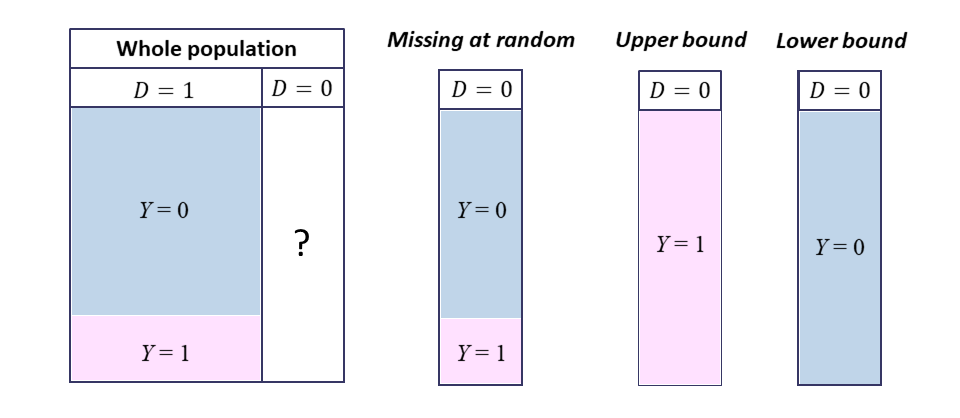
\includegraphics[width=15cm]{partialident.png}
	\end{center}

	In order to obtain a more informative identified interval than $\Theta'_{\E[Y]}$, we need to add more assumptions on $\E [Y \mid D = 0]$.
	For example, suppose that we know that $\E [Y \mid D = 1] \le \E[Y \mid D = 0]$.\footnote{
		For example, let $Y$ be the yes/no answer to a question about the experience of illegal drug use.
		Then, it would be somewhat likely that the respondents who did not answer this question have more experience of drug use ($Y = \text{yes}$) than those who did answer the question.
		Thus, it should be reasonable to assume that $\Pr(Y = \text{yes} \mid D = 1) \le \Pr(Y = \text{yes} \mid D = 0)$ in this example.
	}
	Then, the resulting identified interval for $\E [Y ]$ is
	\[
	\Theta^{\prime\prime}_{\E[Y ]} \equiv \Big[ \E[Y \mid D = 1], \: \E[ Y \mid D = 1] \Pr(D = 1) + \Pr(D = 0) \Big].
	\]
	Clearly, $\Theta^{\prime\prime}_{\E[ Y ]} \subseteq \Theta'_{\E[ Y ]}$.
\end{example}

\begin{example}[Regression with interval-valued dependent variables]\upshape
	It is fairly common that the exact value of variables such as wage or household wealth is not directly asked by surveys; instead, they usually ask the same question in the form of intervals.
	For example, let $Y$ be a wage variable, whose exact level is unknown, but we know that
	\[
	Y \in [Y_L, Y_L + \Delta],
	\]
	where both the value of $Y_L$ and that of $\Delta$ are known, $-\infty < Y_L < \infty$, and $0 < \Delta < \infty$.
	Suppose that we would like to estimate the impact of an explanatory variable $X$ on $Y$ using the following simple 	regression model:
	\[
	Y =  \beta_0 +  \beta_1 X + \eps, \;\; \E[\eps \mid X] = 0.
	\]
	For simplicity, we assume that $\E [X] = 0$.
	Then, if $Y$ were observed, we can identify $\beta_1$ by
	\[
		 \beta_1 = \frac{\E[ XY ]}{\E[X^2]},
	\]
	assuming that $\E [X^2] > 0$.
	When $Y$ is unknown, researchers often try to estimate $\beta_1$ by the sample analog of $\E [X(Y_L + \Delta/2)]/\E[X^2]$.
	However, this approach does not have a theoretical justification.
	\bigskip

	A more conservative and safer approach is to use partial identification. 
	Note that there exists a latent random variable $t \in [0, 1]$ such that
	\[
		Y = Y_L + t \Delta.
	\]
	Thus, we can write
	\[
		\beta_1 = \frac{\E[XY_L]}{\E[X^2]} + \frac{\E[X \cdot t \Delta]}{\E[X^2]}.
	\]
	Observe that
	\begin{align*}
		\E[X \cdot  t\Delta] 
		& =  \E[X \cdot  t \Delta\mbf{1}\{ X > 0 \}] + \E[X \cdot  t \Delta\mbf{1}\{ X < 0\}] \\
		& \le \E[X \cdot  1 \Delta\mbf{1}\{ X > 0 \}] + \E[X \cdot  0 \Delta\mbf{1}\{ X < 0\}] \\
		& =  \E[X \cdot  \Delta\mbf{1}\{ X > 0\}].
	\end{align*}
	This implies that the upper bound of  $\beta_1$ is obtained by
	\[
	 	\beta_1 \le \frac{\E[XY_L]}{\E[X^2]} + \frac{\E[X \cdot \Delta\mbf{1}\{ X > 0\}]}{\E[X^2]}	.
	 \]
	Similarly, we can show that $\E [X \cdot t\Delta] \ge \E[X \cdot \Delta\mbf{1}\{ X < 0\}]$, and thus the lower bound of  $\beta_1$ is
	\[
		\beta_1 \ge \frac{\E[XY_L]}{\E[X^2]} + \frac{\E[X \cdot \Delta\mbf{1}\{ X < 0\}]}{\E[X^2]}.
	\]
	Consequently, we can obtain the identified interval for  $\beta_1$ as
	\[
	\Theta_{\beta_1} \equiv \Bigg[
	\frac{\E[XY_L]}{\E[X^2]} + \frac{\E[X \cdot \Delta \mbf{1}\{ X < 0 \}]}{\E[X^2]},
	\;\;
	\frac{\E[XY_L]}{\E[X^2]} + \frac{\E[X \cdot \Delta\mbf{1}\{ X > 0 \}]}{\E[X^2]}
	\Bigg].
	\]
	From this, we can observe that the length of the identified interval is proportional to $\Delta$.
	For more general discussion on this topic, see \cite{bontemps2012set}
\end{example}

\begin{framed}
\begin{exercise}\upshape
	Consider a simple regression model:
	\[
	Y = \beta_0 + \beta_1 X + \eps, \;\; \E \eps = 0,
	\]
	where the regressor $X$ is suspected to be endogenous: $\Cov(X, \eps) \neq 0$.
	Suppose that we have an ``imperfect'' instrument $Z \in \mbb{R}$ for $X$ such that $\Cov(X, Z) > 0$ and $\underbar c \le \Cov(Z,\eps) \le \bar c$, where $\underbar c$ and $\bar c$ are known constants.
	Derive an informative identified interval for $\beta_1$.
\end{exercise}

\begin{exercise}\upshape
Imagine you are a seller at an online store like Amazon.
You have sold out your products to 300 people at the site.
Among these 300 buyers, 100 of them posted the product's review with a star rating.
The distribution of the star-ratings is as given in Table \ref{table:stars}.
Suppose that you would like to know the value of $\mu \equiv \E[\text{the number of $\star$'s}|\text{buyers}]$.

\begin{enumerate}
	\item If you assume that the missing-at-random (MAR) holds, what is the estimate of $\mu$?
	\item Do you think the MAR assumption is credible in this context? Why?
	\item When imposing no assumptions on the non-respondents, we can only partially identify $\mu$.
	(a) Derive the identified set, and (b) report the computed identified set.
	\item Suppose you would like to obtain a smaller identified set than the one obtained in 3.
	Explain specifically (a) what kind of additional assumption(s) you would introduce and (b) to what extent the resulting identified set is smaller than the one in 3. 
\end{enumerate}
\end{exercise}
\end{framed}

\begin{table}[h]
	\caption{Distribution of star-ratings}\label{table:stars}
	\begin{center}
	\begin{tabular}{c|c}
	\hline
	$\star \star \star \star \star $ & 20 \\
	$\star \star \star \star $ & 32 \\
	$\star \star \star $ & 24 \\
	$\star \star $ & 9 \\
	$\star $ & 15 \\
	\hline
	Total & 100\\
	\hline
	\end{tabular}
	\end{center}
\end{table}

%%%%%%%%%%%%%%%%%%%%%%%%%%%%%%%%%%%%%%%%%%%%%%%%%%%%%%%%%%
%%%%%%%%%%%%%%%%%%%%%%%%%%%%%%%%%%%%%%%%%%%%%%%%%%%%%%%%%%
%%%%%%%%%%%%%%%%%%%%%%%%%%%%%%%%%%%%%%%%%%%%%%%%%%%%%%%%%%

\chapter{Structural Estimation}

One of the most important tasks in econometrics is to empirically simulate the impact of new policies.
However, there is a huge difficulty to quantify the policy impact if the policy is purely hypothetical or there are no similar policies implemented in the past.
In such situations, pure causal inference methods are infeasible simply because we cannot observe data ``after'' the policy.

One possible approach to circumvent this problem is to use a \textbf{structural estimation\index{structural estimation}} technique.
Structural estimation is a method to construct econometric models explicitly based on economic theory and  estimate the parameters of functions (such as utility function, supply function, etc.) that govern the behavior of individuals and firms.
Once these functions are recovered, even when we do not have any data for the policy, we can predict how individuals and firms behave in the hypothetical situation using some economic theory as a guideline.\footnote{
	The idea of structural estimation is closely related to the well-known \textbf{Lucas critique\index{Lucas critique}} of macroeconomic forecasting:
	\begin{quote}\it
		Given that the structure of an econometric model consists of optimal decision-rules of economic agents, and that optimal decision-rules vary systematically with changes in the structure of series relevant to the decision maker, it follows that any change in policy will systematically alter the structure of econometric models. \upshape a quote from \cite{LUCAS197619}.
	\end{quote}
	His statement can be interpreted as that (atheoretical) ``reduced-form'' econometric models should not be used for the purpose of predicting the effect of a new policy.
	Rather, we should model the ``deep'' (i.e., policy invariant) parameters that characterize individual behavior based on microeconomic foundations.
	}

Note that the structural estimation does not refer to a particular estimation method or a type of econometric models.
Rather, it is a way of thinking about econometric models.
As shown below, even a simple OLS regression can be viewed as a structural estimation approach under certain microeconomic assumptions.
Then, the validity of a structural econometric model and its prediction is reduced to the validity of the economic assumptions on which the model is based.

\section{OLS estimation of production functions}
Consider a problem of estimating the agricultural production function of farmers.
For simplicity, suppose that each  farmer has only two inputs, labor $L$ (the number of workers) and capital $K$ (the size of farm land). 
The amount of agricultural output is denoted by $P$.
Then, simply running a linear regression of $P$ on $(L,K)$ is not recognized as a ``structural'' estimation, unless there is a particular reason to believe that the production function is a linear function.
Thus, the obtained regression coefficients cannot be viewed as the estimates of the deep parameters.

A more reasonable (i.e., more justifiable in terms of economic theory) functional form of the production function would be a Cobb--Douglas production function:
\[
	P = A L^\alpha K^\beta,
\] 
where $A$  denotes an idiosyncratic productivity disturbance.
The parameters $\alpha$ and $\beta$ are the output elasticities of labor and capital, respectively.
Taking the log of both sides yields the following linear regression model:
\[
	\log(P) = c + \log(L) \alpha + \log(K) \beta + \eps,
\]
where $c = \E[\log(A)]$, and $\eps = \log(A) - c$.
Hence, by simply running an OLS regression of $\log(P)$ on $(\log(L), \log(K))$, we can estimate the elasticity parameters.

It should be important to note that, although atheoretical (non-structural) estimation approaches cannot be used to simulate counterfactual policy changes, they can be used for the purpose of predicting the other farmers' output level $P$ under the same market condition.
If one's research interest is of the latter type, it is not necessary to consider a structural estimation; rather, it has been shown that using modern \textbf{machine learning} techniques is superior to the classical econometric methods for this purpose (see, e.g., \cite{bajari2015machine}).

\begin{center}
	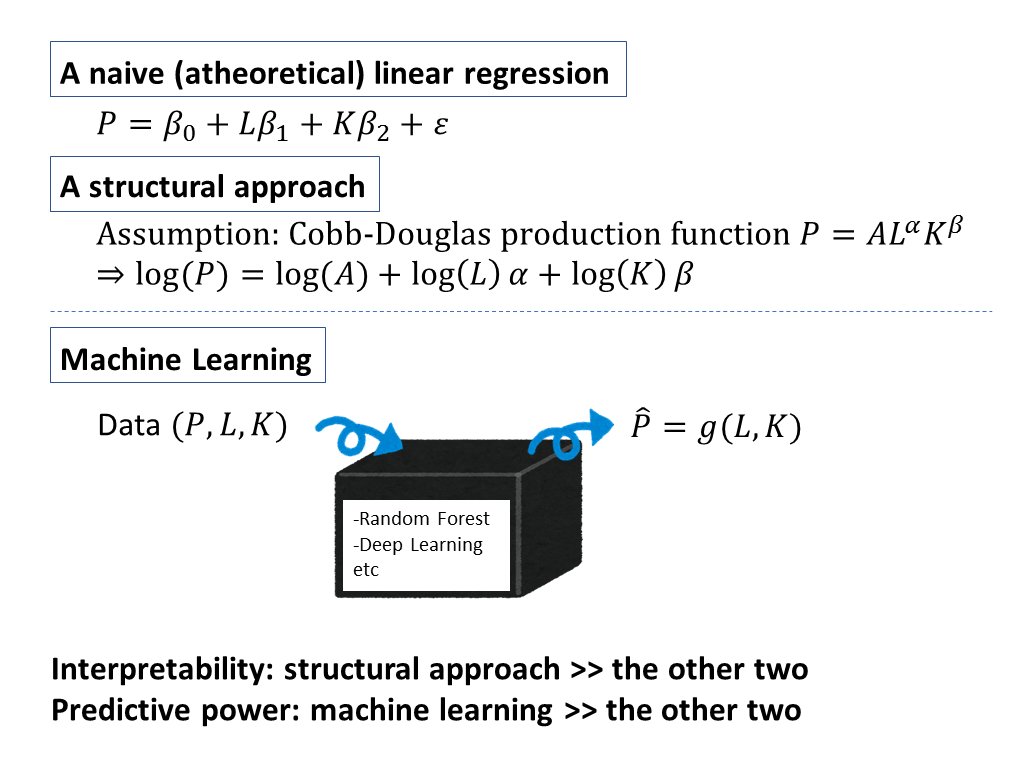
\includegraphics[width = 10.5cm]{prodfunc.png}
\end{center}

\section{Discrete choice models: the random utility framework}

Discrete choice models, such as the logit model, can be viewed as structural econometric models based on the revealed preference approach.
Suppose that there are two goods, say Good 1 and Good 2.
Let $D_i$ be a dummy outcome variable that takes one if consumer $i$ chooses Good 1 and zero if Good 2 is chosen.
Following the revealed preference approach, we can assume that $D_i = 1$ if and only if $U_{i1} > U_{i2}$, where $U_{i1}$ and $U_{i2}$ are the utilities obtained from Good 1 and Good 2, respectively.

For each individual $i$, let $X_i$ be a vector of ``observable'' individual characteristics, and $\eps_{ji}$ be an ``unobservable'' random variable that may be specific to Good $j$.\footnote{
	Note that $\eps_{ji}$ is unobservable only to researchers, but of course $i$ knows the value of her own $\epsilon$.
	}
Then, without loss of generality, we can write $i$'s utility of choosing Good $j$ as $U_{ij} = U_{ij}(X_i, \eps_{ji})$.

Here, unlike the traditional economic model of consumer demand, it is allowed that we cannot fully observe the variables that determine the utility.
Namely, the utility can depend on an unobservable random factor $\eps$.
This framework is called \textbf{random utility model\index{random utility model}} (RUM).\footnote{
	Based on the random utility framework, Daniel McFadden developed a set of econometric methods for analyzing discrete choice behavior. 
	He was awarded the Nobel Prize in economics for this work.
	}
To facilitate the discussion, suppose that the utility function takes the following form:
\[
	U_{ij}(X_i, \eps_{ji}) \equiv V_j(X_i) + \eps_{ji}, \;\; \text{for $j = 1,2$}.
\]
Then, we have
\begin{align*}
	D_i = 1
	& \iff U_{i1}(X_i, \eps_{1i}) > U_{i2}(X_i, \eps_{2i}) \\
	& \iff  V_1(X_i) + \eps_{1i} >  V_2(X_i) + \eps_{2i} \\
	& \iff  V_1(X_i) - V_2(X_i) > \eps_{2i} - \eps_{1i}.
\end{align*}

Now, we assume that the error terms $\eps_{ji}$'s are independent of $X_i$ and are IID as \textbf{Type-1 Extreme Value\index{Type-1 Extreme Value}} (also known as \textbf{Gumbel} distribution).
It is known that the difference of two independent Type-1 Extreme Value variables has the standard logistic distribution.
Therefore, we obtain
\[
	\Pr(D_i = 1 \mid X_i) = \frac{\exp[V_1(X_i) - V_2(X_i)]}{1 + \exp[V_1(X_i) - V_2(X_i)]}.
\]
In applications, we often assume a linear functional form for $V_1(X_i) - V_2(X_i)$ such that
\[
	V_1(X_i) - V_2(X_i) = X_i^\top \beta_0.
\]
for some $\beta_0$.
From this perspective, we can see that the regression coefficient $\beta_0$ in the binary response models corresponds to the difference of the marginal utilities; that is, 
\begin{align*}
	\beta_0 
	& = \frac{\partial V_1(X_i)}{\partial X} - \frac{\partial V_2(X_i)}{\partial X}\\
	& = \frac{\partial U_{i1}(X_i, \eps_{1i})}{\partial X} - \frac{\partial U_{i2}(X_i, \eps_{2i})}{\partial X}
\end{align*}
under the assumptions made here.

\section{Estimation of entry games}\label{sec:games}

In the last few decades, there has been a growing interest in the econometric analysis of game theoretic models (see, e.g., \cite{de2013econometric} for a survey on this topic).
An important early example is the estimation of \textbf{entry games\index{entry games}} (e.g., \cite{bresnahan1990entry,berry1992estimation}).
Suppose that there are two players competing in an entry game across $n$ different markets.
The players are labeled by $j = 1, 2$.
In applications, these labels refer to the actual name of the firms (e.g., JAL and ANA; Walmart and Kmart; IKEA and Nitori). 
A player's entry decision depends on its profit, which in turn depends on whether the rival also enters the market or not.

Let $D_{ij}$ denote whether player $j$ enters the market $i$ ($D_{ij} = 1$) or not ($D_{ij} = 0$), where $i = 1, \ldots, n$.
For each player $j$, we assume that the payoff from entering the market $i$ is given by
\[
	u_{ij}(d_{-j}) \equiv \rho d_{-j} + X_{ij}^\top \beta - \eps_{ij},
\]
where $d_{-j}\in\{0,1\}$ denotes the action chosen by $j$'s opponent, $X_{ij}$ and $\eps_{ij}$ denote observable and unobservable (to econometricians) payoff covariates, and $\rho$ and $\beta$ are the parameters of interest.
We assume that $(\eps_{i1}, \eps_{i2})$ are independent of $(X_{i1}, X_{i2})$ for all $i$.
The parameter $\rho$ captures the \textbf{strategic interaction effect\index{strategic interaction effect}}, in which if it is negative (resp. positive) the model exhibits strategic substitutes (resp. complements).
Note that the parameters $(\rho, \beta)$ can be heterogeneous among the players in general, but we assume that they are homogeneous to simplify the discussion.
Then, the payoff matrix of the game in market $i$ is given by
\begin{center}
\begin{tabular}{c|c|c}
	\hline
	             & $D_{i2} = 0$ & $D_{i2} = 1$ \\ \hline
	$D_{i1} = 0$ & $(0, 0)$     & $(0, X_{i2}^\top \beta - \eps_{i2})$ \\ \hline 
	$D_{i1} = 1$ & $(X_{i1}^\top \beta - \eps_{i1}, 0)$ & $(\rho + X_{i1}^\top \beta - \eps_{i1}, \rho + X_{i2}^\top \beta - \eps_{i2})$\\ \hline
\end{tabular}
\end{center}

Hereinafter, we omit the market index $i$ for simplicity when there is no confusion.
Now, assume that the realizations of $(X_1, X_2)$ and $(\eps_1, \eps_2)$ are known to both players in each market, i.e., we assume a \textbf{complete information game\index{complete information game}}.
Further, we adopt the pure strategy Nash equilibrium as the solution concept of this game.
In addition, suppose that the game is a simultaneous-move game.
Then, we can see that the players' entry decisions follow the following simultaneous binary choice model:
\begin{align}\label{eq:entry}
\begin{split}
D_1 & = \mbf{1}\{\rho D_2 + X_1^\top \beta \geq \eps_1 \} \\
D_2 & = \mbf{1}\{\rho D_1 + X_2^\top \beta \geq \eps_2 \}.
\end{split}
\end{align}
Then, we have the following relationship between the realized outcomes $(D_1, D_2)$ and the error terms $(\eps_1, \eps_2)$:
\begin{equation} \label{eq:equilibrium}
\begin{array}{lcl}
(D_1, D_2) = (1, 1) & \Longrightarrow & \eps_1 \le \rho + X_1^\top \beta, \; \eps_2 \le \rho + X_2^\top\beta, \\
(D_1, D_2) = (1, 0) & \Longrightarrow & \eps_1 \le X_1^\top \beta, \;\;\;\;\;\;\;  \eps_2 > \rho + X_2^\top\beta, \\
(D_1, D_2) = (0, 1) & \Longrightarrow & \eps_1 > \rho + X_1^\top \beta, \; \eps_2 \le X_2^\top\beta, \\
(D_1, D_2) = (0, 0) & \Longrightarrow & \eps_1 > X_1^\top \beta, \;\;\;\;\;\;\; \eps_2 > X_2^\top\beta.
\end{array}
\end{equation}
As conventionally assumed in the literature on entry games, we assume strategic substitutes, i.e., $\rho < 0$.
Then, the relationship in \eqref{eq:equilibrium} can be visually summarized in Figure \ref{fig:nash}.
\begin{figure}[h!]
	\begin{center}
		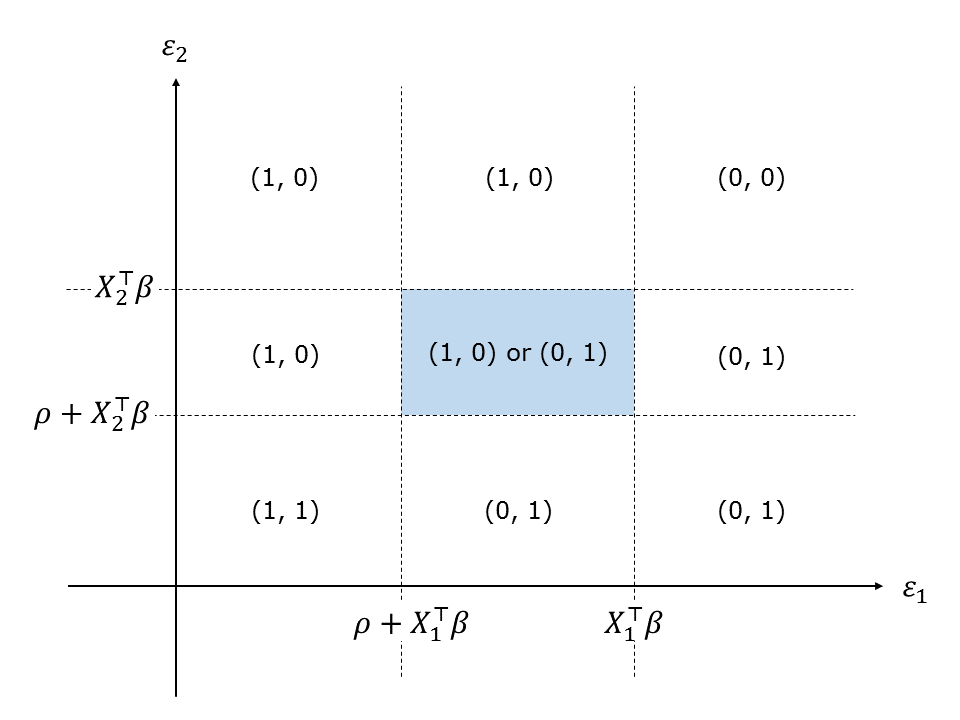
\includegraphics[width = 11cm]{fig_nash.png}
		\caption{Nash equilibrium}
		\label{fig:nash}
	\end{center}
\end{figure}
As shown in the figure, the space of $(\eps_1, \eps_2)$ cannot be partitioned into non-overlapping regions associated with the four alternative realizations of $(D_1, D_2)$.
Both $(D_1,D_2) = (0, 1)$ and $(D_1, D_2) = (1, 0)$ can occur when $(\eps_1, \eps_2)$ fall into the shaded area:
\[
	\begin{array}{l}
		\rho + X_1^\top\beta < \eps_1 \le X_1^\top\beta \\
		\rho + X_2^\top\beta < \eps_2 \le X_2^\top\beta
	\end{array} 
	\begin{array}{ll}
		\Longrightarrow & \text{$(D_1, D_2) = (0,1)$ or $(1,0)$}
	\end{array}
\]
That is, \textbf{multiple Nash equilibria\index{multiple equilibria}} exist in this region.

This non-uniqueness of model-consistent decisions is called \textbf{incompleteness\index{incompleteness}} and has been extensively studied in the literature on simultaneous equations models for discrete outcomes (see, e.g., \cite{tamer2003incomplete}).
When the model is incomplete, the standard maximum likelihood estimation is infeasible because the likelihood function is not well-defined.\footnote{
	If we simply construct the likelihood function based on the relationship \eqref{eq:equilibrium}, then it sums up to a value larger than one.
	}
In what follows, we discuss two approaches to overcome this problem.

\subsection{Rewriting the model in terms of the number of entrants}

Notice that even though there are multiple equilibria in the entry decisions, ``the number of entrants'' can be uniquely determined in our model under $\rho < 0$.
Namely, let $\mbf{N} \in \{0,1,2\}$ be the number of players choosing 1 and $F_j(\cdot)$ and $F(\cdot, \cdot)$ be the marginal and joint distribution function of $\eps_j$'s, respectively.
Then, we have the conditional likelihood function for each action as follows
\begin{align*}
	\text{No entrants} \;\; \Pr(\mbf{N} = 0 \mid X_1, X_2) 
	& = 1 - F_1(X_1^\top\beta) - F_2(X_2^\top\beta) + F(X_1^\top\beta, X_2^\top\beta) \\
	\text{Duopoly} \;\; \Pr(\mbf{N} = 2 \mid X_1, X_2) 
	& = F(\rho + X_1^\top\beta, \rho + X_2^\top\beta) \\
	\text{Monopoly} \;\; \Pr(\mbf{N} = 1 \mid X_1, X_2)
	& = 1 - \Pr(\mbf{N} = 0 \mid X_1, X_2) - \Pr(\mbf{N} = 2 \mid X_1, X_2).  
\end{align*}
Thus, the model can be estimated by solving the following maximum likelihood problem:
\[
	\max_{(\rho, \beta, \ldots)} \sum_{i = 1}^n \sum_{k \in \{0,1,2\}} \mbf{1}\{\mbf{N}_i = k\} \log \Pr(\mbf{N}_i = k \mid X_{i1}, X_{i2}).
\]
Here, the set of estimation parameters may include not only $\rho$ and $\beta$ but also some additional parameters, such as a correlation parameter between $\eps_1$ and $\eps_2$. 
This approach is pursued in \cite{bresnahan1990entry} and \cite{berry1992estimation}, which highlights that the presence of multiple equilibria does not necessarily imply the lack of point identification.

\subsection{Stochastic equilibrium selection rule}\label{subsec:stochastic}

An alternative approach is to explicitly introduce a stochastic (or possibly deterministic) equilibrium selection mechanism. 
Unlike the above approach, this approach allows us to identify the entry behavior in the region of multiplicity.
The simplest form of this approach is to assume a pure random equilibrium selection.
More specifically, suppose that the players would choose $(D_1, D_2) = (1,0)$ with probability $\lambda$ when in the multiple equilibria region.
Then, the likelihood function for each realization can be well-defined as follows:
\begin{align*}
	\Pr(0, 0 \mid X_1, X_2) 
	& = 1 - F_1(X_1^\top\beta) - F_2(X_2^\top\beta) + F(X_1^\top\beta, X_2^\top\beta)  \\
	\Pr(1, 1 \mid X_1, X_2) 
	& = F(\rho + X_1^\top\beta, \rho + X_2^\top\beta) \\
	\Pr(0, 1 \mid X_1, X_2) 
	& = F_2( X_2^\top\beta) - F(\rho + X_1^\top\beta, X_2^\top\beta) - \lambda P_{mul}(X_1, X_2) \\
	\Pr(1, 0 \mid X_1, X_2)
	& = 1 - \sum_{(d_1, d_2) \in \{(0,0), (1,1), (0,1)\}}\Pr( d_1, d_2 \mid X_1, X_2), 
\end{align*}
where
\[
	P_{mul}(X_1, X_2) \equiv F(X_1^\top\beta, X_2^\top\beta)  - F(\rho + X_1^\top\beta, X_2^\top\beta) - F(X_1^\top\beta, \rho + X_2^\top\beta) +   F(\rho + X_1^\top\beta, \rho + X_2^\top\beta) ,
\]
which is the probability that $(\eps_1, \eps_2)$ reside in the multiple equilibria region for given $(X_1, X_2)$.
Then, we can estimate the model by solving the following maximum likelihood problem:
\[
	\max_{(\rho, \beta, \lambda, \ldots)} \sum_{i = 1}^n \sum_{(d_1, d_2) \in \{0,1\}^2} \mbf{1}\{(D_{i1}, D_{i2}) = (d_1, d_2) \} \log \Pr( d_1, d_2 | X_{i1}, X_{i2}).
\]

\subsection{When the sign of $\rho$ is unknown}

So far, we have assumed that the sign of the strategic interaction effect is known a priori.
Although such assumption may be justified by economic theory in particular situations, in general, we do not have prior knowledge about $\rho$.
When the the sign of $\rho$ is unknown, it is difficult to obtain point identification of the model.

To tackle this problem, \cite{ciliberto2009market} proposed a partial identification approach.
For each realization $(D_1, D_2) = (d_1, d_2)$, we can generally write
\begin{align*}
	\Pr(d_1, d_2 \mid X_1, X_2) 
	& = \int \Pr(d_1, d_2 \mid X_1, X_2, \eps_1, \eps_2) \text{d}F \\
	& = \int_{\mcl{R}_{uni}^{(d_1, d_2)}(X_1, X_2)} \Pr(d_1, d_2 \mid X_1, X_2, \eps_1, \eps_2) \text{d}F + \int_{\mcl{R}_{mul}^{(d_1, d_2)}(X_1, X_2)} \Pr(d_1, d_2 \mid X_1, X_2, \eps_1, \eps_2) \text{d}F \\
	& = \int_{\mcl{R}_{uni}^{(d_1,d_2)}(X_1,X_2)} \text{d}F + \int_{\mcl{R}_{mul}^{(d_1, d_2)}(X_1,X_2)} \Pr(d_1, d_2 \mid X_1, X_2, \eps_1, \eps_2) \text{d}F.
\end{align*}
Here, $\mcl{R}_{uni}^{(d_1,d_2)}(X_1, X_2)$ denotes the region of $(\eps_1, \eps_2)$ where $(D_1, D_2) = (d_1, d_2)$ uniquely occurs for given $(X_1, X_2)$, and $\mcl{R}_{mul}^{(d_1,d_2)}(X_1, X_2)$ is the multiple equilibria region.
The probability function $\Pr(d_1, d_2 \mid X_1, X_2, \eps_1, \eps_2)$ plays the role of equilibrium selection function for $(d_1, d_2)$ in the multiplicity region.\footnote{
	If we can impose some parametric functional form assumption on $\Pr(d_1, d_2 \mid X_1, X_2, \eps_1, \eps_2)$ for $(\eps_1, \eps_2) \in \mcl{R}_{mul}^{(d_1, d_2)}(X_1,X_2)$, then we may point identify the model.
	Such an approach was taken in \cite{bajari2010identification}.
}
Whatever the functional form of $\Pr(d_1, d_2 \mid X_1, X_2, \eps_1, \eps_2)$ is, since $0 \le \Pr(d_1, d_2 \mid X_1, X_2, \eps_1, \eps_2) \le 1$ must hold, we have
\begin{align}\label{eq:gameinequality}
	\int_{\mcl{R}_{uni}^{(d_1,d_2)}(X_1,X_2)} \text{d}F
	\le \Pr(d_1, d_2 \mid X_1, X_2) 
	\le \int_{\mcl{R}_{uni}^{(d_1,d_2)}(X_1,X_2)} \text{d}F + \int_{\mcl{R}_{mul}^{(d_1, d_2)}(X_1,X_2)} \text{d}F. 
\end{align}
Thus, the identified set of the model parameters can be defined by the set of parameters that satisfy \eqref{eq:gameinequality}.
For practical implementation of this approach, see \cite{ciliberto2009market}.

\section{Estimation of first-price auction models}

To be added in a future update.

\section{BLP Demand Estimation}

To be added in a future update.

%%%%%%%%%%%%%%%%%%%%%%%%%%%%%%%%%%%%%%%%%%%%%%%%%%%%%%%%%%
%%%%%%%%%%%%%%%%%%%%%%%%%%%%%%%%%%%%%%%%%%%%%%%%%%%%%%%%%%
%%%%%%%%%%%%%%%%%%%%%%%%%%%%%%%%%%%%%%%%%%%%%%%%%%%%%%%%%%

\chapter{Bootstrap}

The bootstrap is a method to estimate the distribution of an estimator or that of a test statistic by repeatedly resampling the original data.
The bootstrap was introduced by \cite{efron1979bootstrap} and has continued to be one of the central interests of statistical research in all areas.
The bootstrap has several advantages over the classical inference methods that are based on the asymptotic distributions.
One is its algorithmic simplicity.
It is often the case that in complicated econometric models, the statistic of interest has a very complicated form of asymptotic variance, which makes its estimation cumbersome.
If we use a bootstrap method instead, we may circumvent such complicated computation.
A more important  advantage of using bootstrap is that under some regularity conditions, the approximated distribution obtained by the bootstrap is at least as accurate as and often more accurate than the approximation obtained in the first-order asymptotic theory.
That is, the bootstrap is not just a convenient alternative to the conventional asymptotic method, but it sometimes exhibits theoretically desirable properties compared to the conventional method.

The contents of this chapter are mostly based on \cite{HOROWITZ20013159} and \cite{horowitz2019bootstrap}.
Detailed mathematical proofs will be omitted.\footnote{For those who are interested in the theory of bootstrap, I suggest take a look at \cite{hall1992bootstrap} first, among many others.}

\section{The basic idea of the bootstrap method}

Suppose that we have an IID sample $\{X_1, \ldots, X_n\}$ of size $n$ obtained from an unknown distribution $F_0$.
Let $T_n \equiv T_n(X_1, \ldots, X_n)$ be the statistic of which we would like to know the distribution.
A conventional approach is to derive its asymptotic distribution as $n \to \infty$.
For example, let $T_n$ be the $t$-statistic for testing the null hypothesis $\mathbb{H}_0: \E X = 0$; namely,
\begin{align*}
	T_n = \frac{\bar X_n}{s_n},
\end{align*}
where $\bar X_n$ amd $s_n$ are the sample mean and sample standard deviation, respectively.
Then, by CLT, we know that $T_n$ is distributed as the standard normal $N(0,1)$ as $n \to \infty$.
This approximation is actually very accurate if the sample size is not small.
However, for more involved test statistics in complicated models, the asymptotic approximation can be inaccurate for moderate sample sizes.

Now, consider a general statistic $T_n$ and let $G_n(\cdot \mid F)$ be the distribution function of $T_n$ when the data are drawn from the distribution function $F$:
\begin{align*}
	G_n(t \mid F) 
	& \equiv P_F(T_n(X_1, \ldots, X_n) \le t) \\
	& = \int \mbf{1}\{T_n(x_1, \ldots, x_n) \le t\} \mathrm{d} F^n.
\end{align*}
The true distribution of $T_n$ under $F_0$ can be written as $G_n(\cdot \mid F_0)$.
Thus, if we happen to know the exact form of $G_n(\cdot \mid F_0)$, we can conduct any statistical inference on $T_n$; however, this is a rare case since $F_0$ is usually unknown.\footnote{
	For example, in a randomized experiment setup where any randomness comes only through the treatments, it is possible to know the exact distribution of a test statistic (cf., Fisher's randomization test).
}

For data $\{X_1, \ldots, X_n\}$ that are drawn from $F_0$, we have the empirical distribution function $F_n$ of $X$ (as an approximate of $F_0$) as
\begin{align*}
	F_n(t) \equiv \frac{1}{n}\sum_{i = 1}^n \mbf{1}\{X_i \le t\}.
\end{align*} 
Using this empirical distribution, we can compute $G_n(\cdot \mid F_n)$, instead of $G_n(\cdot \mid F_0)$, in the following manner:
\begin{description}
	\item[Step 1.] Generate a bootstrap sample $\{X_1^*, \dots, X_n^*\}$ from $F_n$. 
	\item[Step 2.] Compute the test statistic $T_n^* = T_n(X_1^*, \dots, X_n^*)$.
	\item[Step 3.] Repeat Steps 1 and 2 many times, and compute the empirical distribution of $T_n^*$. 
\end{description}
Note that the empirical distribution $F_n$ is just a discrete uniform distribution that assigns probability $1/n$ on each observed value.
Thus, Step 1 can be simply performed by a simple random sampling from $\{X_1, \ldots, X_n\}$ with replacement.
By increasing the number of repetitions in Step 3, we can approximate $G_n(\cdot \mid F_n)$ arbitrarily precisely.\footnote{
	Note that, theoretically, the exact form of $G_n(t \mid F_n)$ can be obtained by calculating the proportion of all possible bootstrap samples that have $\{T_n^* \le t\}$.
	However, this would require $n^n$ calculations, which is not possible in practice except when $n$ is very small.
	Thus, in Step 3, we basically generate ``as many bootstrap samples as possible''.
}
The above procedure is called the \textbf{nonparametric bootstrap\index{nonparametric bootstrap}}.

By a uniform LLN, we have $|F_n(z) - F_0(z)| = o_P(1)$ over all $z$.
Formally, this result is known as the \textbf{Glivenko-Cantelli theorem}.
From this result, for sufficiently large $n$, we can anticipate that $G_n(\cdot \mid F_n) \approx G_n(\cdot \mid F_0)$ in some sense if $G_n$ is continuous in $F$.
This is the consistency property of bootstrap.
A more formal definition is as follows.

Taking the limit $n \to \infty$ of $G_n(\cdot \mid F_0)$, we define the asymptotic true distribution of $T_n$ as $G_\infty(\cdot \mid F_0)$.
\begin{definition}[Bootstrap consistency]
	The bootstrap distribution estimator $G_n(\cdot \mid F_n)$ is said to be \textbf{consistent\index{Bootstrap consistency}} if, for any $\kappa > 0$,
	\begin{align*}
		\Pr \left(\; |G_n(t \mid F_n) - G_\infty( t \mid F_0)| > \kappa \;\; \text{for all } t \in \mathbb{R} \right) \to 0.
	\end{align*}
\end{definition}
Note that in the above definition, the bootstrap distribution $G_n(t \mid F_n) = P_{F_n}(T_n(X_1^*, \ldots, X_n^*) \le t)$ is a random CDF because $F_n$ depends on the original sampling $\{X_1, \ldots, X_n\}$.
Thus, the probability is taken over this randomness.
$G_\infty(\cdot \mid F_0)$ is not a stochastic function.
Once a consistent bootstrap distribution $G_n(\cdot \mid F_n)$ is obtained, we can perform statistical inference based on the bootstrap critical values and the confidence intervals directly obtained from $G_n(\cdot \mid F_n)$.

\begin{figure}[h!]
	\begin{center}
		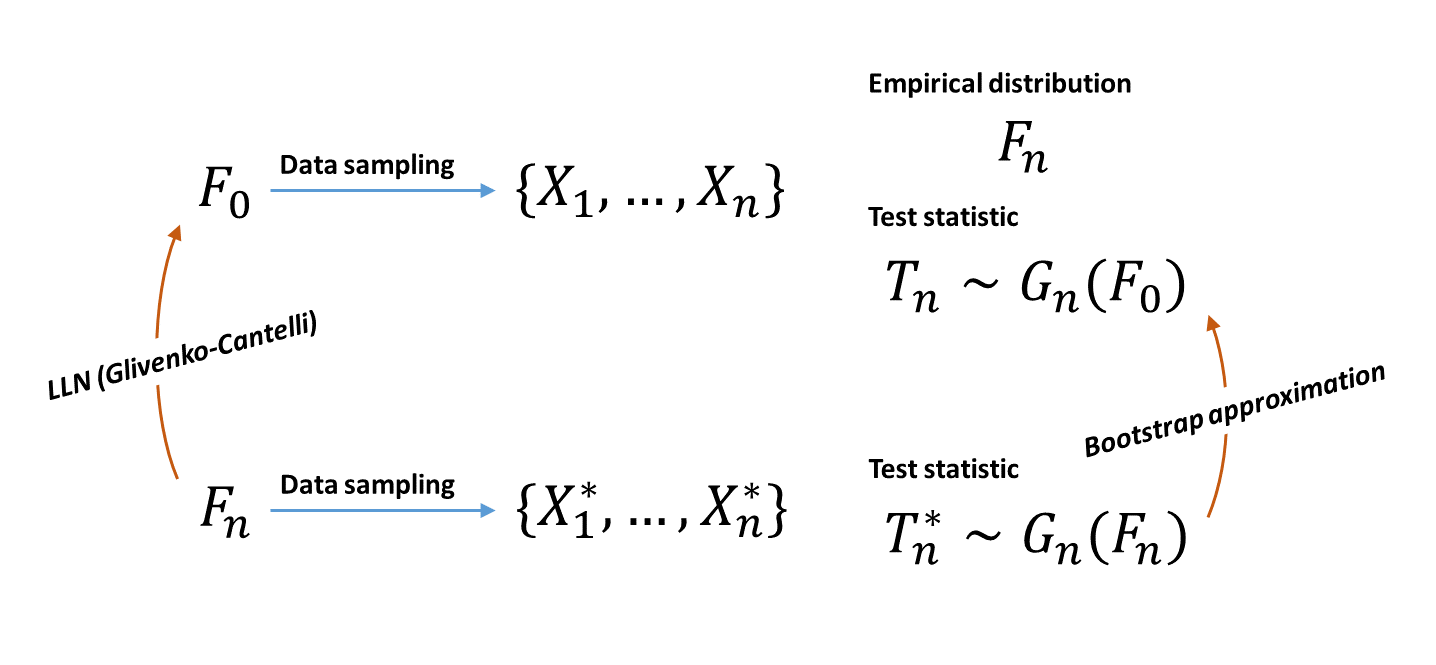
\includegraphics[width = 13cm]{bootstrap.png}
		\caption{The idea of bootstrap}
	\end{center}
\end{figure}

It is difficult to provide general and easy-to-check conditions for a bootstrap estimator to be consistent.
In many practical situations, it is often the case that the test statistic of interest can be expressed as $T_n = (\bar g_n - t_n)/s_n$ for some sequences $t_n$ and $s_n$, where $\bar g_n = n^{-1}\sum_{i = 1}^n g(X_i)$ with an IID sample $\{X_1, \ldots, X_n\}$.
For this special case, \cite{mammen1992bootstrap} shows that the nonparametric bootstrap distribution of $T_n^* = (\bar g_n^* - \bar g_n)/s_n$, where $\bar g_n^* = n^{-1}\sum_{i = 1}^n g(X^*_i)$, is consistent for the distribution of $T_n$ if and only if $T_n \overset{d}{\to} N(0,1)$.
Many of commonly used estimators and test statistics, such as least squares estimators, ML estimators, $t$-statistic, etc, have this form and are asymptotically normal.
Thus, the nonparametric bootstrap is consistent for most applications.
Nonetheless, it is important to know when the bootstrap may fail.

One such example is the estimation of the distribution of the maximum or minimum value of a sample.
Let $\{X_1, \ldots, X_n\}$ be an IID sample drawn from $\mathrm{Uniform}[0, \alpha_0]$.
As we have seen in Exercise \ref{ex:maxuni}, the ML estimator of $\alpha_0$ is given by 
\begin{align*}
	\hat \alpha_n^{mle} = \max\{X_1, \ldots, X_n\}. 
\end{align*}
Define $T_n \equiv n(\alpha_0 - \hat \alpha_n^{mle})/\alpha_0$.
One can show that the limiting distribution of $T_n$ is the standard exponential.
In particular, we have $\Pr(T_n = 0) = 0$ for all $n$.

Now, let $\{X_1^*, \ldots, X_n^*\}$ be a bootstrap sample that is obtained by sampling the original data $\{X_1, \ldots, X_n\}$ randomly with replacement.
Then, the bootstrap analog of $T_n$ is $T_n^* \equiv n(\hat \alpha_n^{mle} - \hat \alpha_n^*)/\hat \alpha_n^{mle}$, where $\hat \alpha_n^* = \max\{X_1^*, \ldots, X_n^*\}$ (note that the ``population'' value for the upper bound of the bootstrap samples is $\hat \alpha_n^{mle}$).
Hence,
\begin{align*}
	P_{F_n}(T_n^* = 0)
	& = \int \mbf{1}\{\hat \alpha_n^* = \hat \alpha_n^{mle}\} \mathrm{d} F_n^n\\
	& = \int (1 - \mbf{1}\{\text{$\hat \alpha_n^{mle} \not\in $ bootstrap sample}\}) \mathrm{d} F_n^n\\
	& = 1 - (1 - (1/n))^n \to 1 - e^{-1}.
\end{align*}
Thus, the bootstrap distribution of $T_n^*$ is not consistent for the distribution of $T_n$.
This result would be intuitively understandable noting the fact that the bootstrap maximum never exceeds the maximum of the original sample.

As in the above example, when the target parameter is on a boundary, simple nonparametric bootstrap methods often fail.
For other examples, see \cite{HOROWITZ20013159} and \cite{horowitz2019bootstrap}

\section{Asymptotic refinements}

Let $\{\mbf{X}_1, \ldots, \mbf{X}_n\}$ be an IID sample from the distribution of the random vector $\mbf{X} \sim F_0$.
Further, let $\mbf{Z}(\cdot)$ be a vector-valued function of $\mbf{X}$, and define $\zeta \equiv \E [\mbf{Z}(\mbf{X})]$, $\mbf{Z}_i \equiv \mbf{Z}(\mbf{X}_i)$, and $\bar{\mbf{Z}} \equiv n^{-1} \sum_{i = 1}^n \mbf{Z}_i$.
The parameter of interest is $H(\zeta)$ and we estimate it by $H(\bar{\mbf{Z}})$.

For example, for a simple linear regression with a standardized regressor, we have the slope parameter $\beta = H(\zeta)$ and its estimate $\hat \beta = H(\bar{\mbf{Z}})$, where $\mbf{X} = (X, Y)$, $\mbf{Z}(\mbf{X}) = (X Y , X^2 )$, 
\begin{align*}
	\zeta = \biggl(\underbrace{\E[XY]}_{\zeta_1}, \underbrace{\E[X^2]}_{\zeta_2}\biggr), 
	\;\; \bar{\mbf{Z}} = \biggl(\underbrace{\frac{1}{n} \sum_{i = 1}^n X_i Y_i}_{\bar{\mbf{Z}}_1}, \underbrace{\frac{1}{n} \sum_{i = 1}^n X_i^2}_{\bar{\mbf{Z}}_2} \biggr),
	\;\;
	H(\zeta) = \frac{\zeta_1}{\zeta_2}, 
	\;\;  H(\bar{\mbf{Z}}) = \frac{\bar{\mbf{Z}}_1}{\bar{\mbf{Z}}_2}.
\end{align*}

In the following, we focus on estimating the distribution of the statistic
\begin{align*}
	T_n = \frac{\sqrt{n}(H(\bar{\mbf{Z}}) - H(\zeta))}{s_n},
\end{align*}
where $s_n^2$ is a consistent estimator of the variance of $\sqrt{n}(H(\bar{\mbf{Z}}) - H(\zeta))$.
We assume that $H$ is sufficiently smooth such that it has sufficiently many derivatives.
In addition, we assume the following condition:

\paragraph{Cram\'{e}r Condition} 
Let $\tau$ be a vector of constants with the same dimension as $\mbf{Z}$.
Let $i \equiv \sqrt{-1}$.
$\mbf{Z}$ satisfies the Cram\'{e}r condition:
\begin{align*}
	\limsup_{||\tau || \to \infty} |\E \exp(i \tau^\top \mbf{Z})| < 1. 
\end{align*} 
That is,  the Cram\'er condition requires that the absolute value of the characteristic function $\phi_\mbf{Z}(\tau) \equiv \E \exp(i \tau^\top \mbf{Z})$ is strictly bounded by one uniformly in $\tau$.
This condition is satisfied if $\mbf{Z}$ is continuous and has a proper density function.\footnote{
	Note that $|\phi_\mbf{Z}(\tau)| \le 1$ always holds for all $\tau$:
	\begin{align*}
		|\phi_\mbf{Z}(\tau)| 
		& \le \E | \exp(i \tau^\top \mbf{Z})| \\
		& = \E |\cos(\tau^\top \mbf{Z}) + i \sin (\tau^\top \mbf{Z})| \;\; (\text{Euler's formula}) \\
		& = \E\left[  (\cos^2(\tau^\top \mbf{Z}) +  \sin^2(\tau^\top \mbf{Z}))^{1/2} \right] = 1.
	\end{align*}
	For a formal derivation of the Cram\'er condition, see, e.g., Section 2.4 of \cite{hall1992bootstrap}.
}

Let $G_n(\cdot \mid F_0)$ and $G_\infty(\cdot \mid F_0)$ denote the distribution and the asymptotic distribution of $T_n$, respectively.
Similarly, $G_n(\cdot \mid F_n)$ and $G_\infty(\cdot \mid F_n)$ are defined as the bootstrap counterparts of $G_n(\cdot \mid F_0)$ and $G_\infty(\cdot \mid F_0)$, respectively.
Then, under the Cram\'er condition, we have the following result:
\begin{align}\label{eq:edgeworth}
	\begin{split}
		\underset{\text{target}}{G_n(t \mid F_0)} & = \underset{\text{asymp dist}}{G_\infty(t \mid F_0)} + \frac{1}{n^{1/2}} g_1(t, F_0) + \frac{1}{n} g_2(t, F_0) + \frac{1}{n^{3/2}} g_3(t, F_0) + O(n^{-2}) \\
		\underset{\text{boot dist}}{G_n(t \mid F_n)} & = G_\infty(t \mid F_n) + \frac{1}{n^{1/2}} g_1(t, F_n) + \frac{1}{n} g_2(t, F_n) + \frac{1}{n^{3/2}} g_3(t, F_n) + O(n^{-2}) 
	\end{split}
\end{align}
uniformly over $t$.
Here, $g_1$ and $g_3$ are even functions and $g_2$ is an odd function with respect to the first argument.
The series expansion of a distribution function given in \eqref{eq:edgeworth} is called an \textbf{Edgeworth expansion\index{Edgeworth expansion}}.
From this result, we can see that the conventional asymptotic method that approximates $G_n(t \mid F_0)$ by its asymptotic analog $G_\infty(t \mid F_0)$ has an approximation error of order $O(n^{-1/2})$.

Note that in our setup, both $T_n \overset{d}{\to} N(0,1)$ and $T_n^* \overset{d}{\to} N(0,1)$ hold.
That is, the first terms on the right-hand side of \eqref{eq:edgeworth} are both $\Phi(t)$, the standard normal CDF.
When the asymptotic distribution of a statistic does not depend on the DGP, such as $G_\infty(t \mid F) = N(0,1)$ for any $F$ as in the present case, we say that the statistic is \textbf{asymptotically pivotal\index{asymptotically pivotal}}.
Most test statistics are asymptotically pivotal, but most estimators are not.

Then, it follows from \eqref{eq:edgeworth} that the gap between the true distribution and the bootstrap distribution is 
\begin{align*}
	G_n(t \mid F_0) - G_n(t \mid F_n) 
	& = \frac{1}{n^{1/2}}[g_1(t, F_0) - g_1(t, F_n)] + \frac{1}{n}[g_2(t, F_0) - g_2(t, F_n)] + O(n^{-3/2}).
\end{align*}
The leading term on the right-hand side is $n^{-1/2}[g_1(t, F_0) - g_1(t, F_n)]$.
Since $F_n$ converges to $F_0$, this term converges to zero faster than $n^{-1/2}$.
Indeed, one can show that $[g_1(t, F_0) - g_1(t, F_n)] = O(n^{-1/2})$, and therefore the approximation error by the bootstrap is of order $O(n^{-1})$, i.e., an \textbf{asymptotic refinement\index{asymptotic refinement}}.
Thus, the bootstrap is more accurate than the conventional asymptotic approximation.
\bigskip

The bootstrap is even more accurate when approximating the symmetrical distribution $\Pr(|T_n| \le t)$.
Noting that $g_1$ and $g_3$ are even functions and $g_2$ is an odd function (i.e., $g_1(t, F) = g_1(-t, F)$, $g_2(t, F) = - g_2(-t, F)$, and $g_3(t, F) = g_3(-t, F)$) and that $\Phi(-t) = 1 - \Phi(t)$,
\begin{align*}
	P_{F_0}(|T_n| \le t) 
	& = P_{F_0}(T_n \le t) -  P_{F_0}(T_n \le - t) \\
	& = G_n(t \mid F_0) - G_n( - t \mid F_0) \\
	& = \Phi(t) - \Phi(-t) + \frac{1}{n^{1/2}}[g_1(t, F_0) - g_1(-t, F_0)] + \frac{1}{n}[g_2(t, F_0) - g_2(-t, F_0)] \\
	& \quad + \frac{1}{n^{3/2}} [g_3(t, F_0) - g_3(-t, F_0)] + O(n^{-2}) \\
	& = 2 \Phi(t) - 1 + \frac{2}{n}g_2(t, F_0) + O(n^{-2}).
\end{align*}
Similarly,
\begin{align*}
	P_{F_n}(|T_n^*| \le t) 
	& = 2 \Phi(t) - 1 + \frac{2}{n}g_2(t, F_n) + O(n^{-2}).
\end{align*}
Further, similarly as above, one can show that $[g_2(t, F_0) - g_2(t, F_n)] = O(n^{-1/2})$.
Thus, the error in the bootstrap approximation to the symmetrical distribution is $O(n^{-3/2})$.

Note that if the statistic $T_n$ is not asymptotically pivotal (for example when a non-standardized $T_n = \sqrt{n}(H(\bar{\mbf{Z}}) - H(\zeta))$ is used), the leading term of the difference $G_n(t \mid F_0) - G_n(t \mid F_n)$ will be $G_\infty(t \mid F_0) - G_\infty(t \mid F_n)$, which is typically of order $O(n^{-1/2})$.
Then, in this case, the error of the bootstrap approximation converges to zero at the same rate as that of the conventional asymptotic approximation (i.e., no asymptotic refinements); that is, there is no merit of using bootstrap other than computational simplicity.

\begin{table}[h]
	\caption{Approximation errors for estimating $G_n(\cdot \mid F_0)$}
	\begin{tabular}{l|cccc}
		\hline
	& Asymptotic distribution     & \multicolumn{3}{c}{Bootstrap}    \\
    &                             & Pivotal                   & Pivotal + Symmetricity         & Not pivotal                 \\
		\hline
	The order of approximation error & $n^{-1/2}$ & $n^{-1}$ & $n^{-3/2}$ & $n^{-1/2}$ \\
		\hline
	\end{tabular}
\end{table}

\section{Other bootstrap resampling schemes}
\subsection{Parametric bootstrap}

The consistency property of the nonparametric bootstrap method is essentially a consequence of the consistency of $F_n$ for $F_0$.
Moreover, the size of the error in the bootstrap approximation is determined by the size of $|F_n - F_0|$.
Thus, to improve the performance of bootstrap, $F_n$ should be obtained by the most efficient available estimator.
Clearly, if we know the form of $F_0$ perfectly, we should use $F_0$ to generate bootstrap samples, rather than $F_n$.
When it is known that $F_0$ belongs to a parametric family with some unknown parameters $\theta$ such that $F_0(\cdot) = F(\cdot ; \theta_0)$, we can use $F(\cdot ; \theta_n)$ as a bootstrap sample generator with $\theta_n$ being a consistent estimator of $\theta_0$ such as an ML estimator.
This approach is called the \textbf{parametric bootstrap\index{parametric bootstrap}}.

\subsection{Residual bootstrap}

Suppose that we are interested in estimating the regression model
\begin{align*}
	Y_i = X_i^\top \beta_0 + \eps_i, \;\; \E(\eps_i \mid X_i) = 0.
\end{align*}
We assume that the data $\{(X_i, Y_i) : 1 \le i \le n\}$ are IID such that $\E(\eps_i^2) = \sigma^2$ (i.e., homoskedasticity).
$\mbf{X}_i$ includes a constant term.
For this setup, we can generate bootstrap samples in the following manner:
\begin{description}
	\item[Step 1.] Obtain the OLS estimate $\hat \beta_n$ of $\beta_0$.
	\item[Step 2.] Compute the residuals $\hat \eps_i = Y_i - X_i^\top \hat \beta_n$ for all $i= 1, \ldots, n$.
	\item[Step 3.] Create a bootstrap sample $\{(Y_i^*, X_i): 1 \le i \le n\}$, where $Y_i^* = X_i^\top \hat \beta_n + \hat \eps_i^*$, and $\eps^*_i$'s are obtained by a random sampling from $\{\hat \eps_1, \ldots, \hat \eps_n\}$ with replacement.
\end{description}
In the above procedure, only the residuals are resampled repeatedly to create bootstrap samples, and the regressors $X_i$'s are the same as the original sample and are not resampled.
This approach is called the \textbf{residual bootstrap\index{residual bootstrap}}.
Note that in Step 3, we implicitly assume that the errors are identically distributed.

If we know the exact form of the distribution function of the error terms, as in the parametric bootstrap, we can draw new error terms from it, rather than sampling from the residuals.
Such a situation is common in parametric limited dependent variable models such as probit and logit.

\subsection{Wild bootstrap}

We continue to consider the same regression model as above.
However, we now assume that the error terms are heteroskedastic: $\E(\eps_i^2) = \sigma_i^2$.
In this case, using the residual bootstrap is not appropriate.

Letting $\hat \beta_n$ denote the OLS estimate of $\beta_0$ and $\hat \eps_i = Y_i - X_i^\top \hat \beta_n$, the \textbf{wild bootstrap\index{wild bootstrap}} generates new $Y_i^*$'s as $Y_i^* = X_i^\top \hat \beta_n + u_i^*$, where
\begin{align*}
	u_i^* \equiv W_i \hat \eps_i, \;\; i = 1, \ldots, n
\end{align*}
and $\{W_i: 1 \le i \le n\}$ is a randomly generated IID sequence that is independent of the whole data and satisfies $\E W_i = 0$ and $\E W_i^2 = 1$.
Common choices of distributions for $W_i$ include the standard normal and the two-point distribution that takes $(1 - \sqrt{5})/2$ with probability $(\sqrt{5} + 1)/(2 \sqrt{5})$ and $(\sqrt{5} + 1)/2$ with probability $(\sqrt{5} - 1)/(2 \sqrt{5})$.
It can be easily confirmed that
\begin{align*}
	\E [u_i^* \mid \{(X_j, Y_j)\}_{j=1}^n] 
	& = \E [W_i \mid \{(X_j, Y_j)\}_{j=1}^n]  \hat \eps_i = 0 \\
	\E [(u_i^*)^2 \mid \{(X_j, Y_j)\}_{j=1}^n] 
	& = \E [W_i^2  \mid \{(X_j, Y_j)\}_{j=1}^n]  \hat \eps_i^2 =  \hat \eps_i^2.
\end{align*}
Hence, the heteroskedasticity in the original sample is maintained in the bootstrap sample.

%%%%%%%%%%%%%%%%%%%%%%%%%%%%%%%%%%%%%%%%%%%%%%%%%%%%%%%%%%
%%%%%%%%%%%%%%%%%%%%%%%%%%%%%%%%%%%%%%%%%%%%%%%%%%%%%%%%%%
%%%%%%%%%%%%%%%%%%%%%%%%%%%%%%%%%%%%%%%%%%%%%%%%%%%%%%%%%%

\chapter{Nonparametric Regression}\label{chap:nonpara}

Consider a general regression model: $Y = g(X) + \eps$.
As shown in \eqref{eq:msemin}, in terms of minimization of MSE, the best regression function is the conditional expectation function: $g(X) = \E[Y \mid X]$.
A linear regression model $Y = X^\top\beta + \eps$ is a special case when we impose a funcitonal form  assumption $g(X) = X^\top \beta$, and thus its optimality hinges on whether the assumption $\E[Y \mid X] = X^\top\beta$ is satisfied or not.
In reality, however, it would be extremely rare that the data follow such a linear relationship exactly, and if the functional form assumption does not hold, what the linear regression produces is only a ``linear approximation" of $\E[Y \mid X]$.
As shown in the figure below, linear approximation is not always informative and sometimes even misleading.

\begin{figure}[h!]
	\begin{center}
		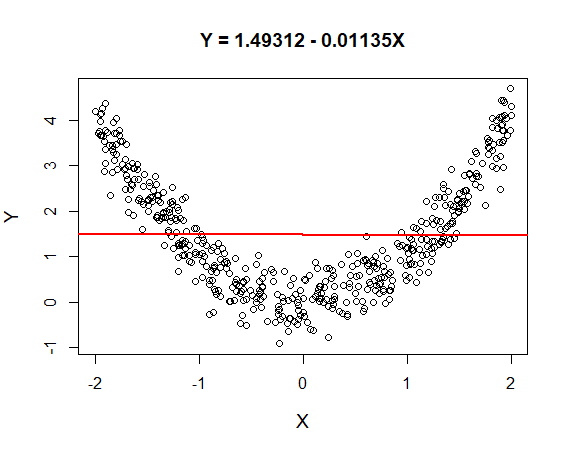
\includegraphics[width = 8cm]{reg.png}
		\caption{Linear approximation of a quadratic function}
	\end{center}
\end{figure}


Thus, ideally, we would like to estimate $\E [Y \mid X]$ without imposing any a priori functional form assumptions.
Such a regression approach is called \textbf{nonparametric\index{nonparametric}}.
In contrast, if one assumes a specific functional form $g(X, \theta)$ with a finite dimensional parameter vector $\theta$, this approach is \textbf{parametric\index{parametric}}.
The most typical parametric regression models are linear regression models.
For another example, if the range of a dependent variable is restricted to $(0,1)$, a logistic regression model $g(X, \theta) = \exp(X^\top \theta)/[1 + \exp(X^\top \theta)]$ is popularly used. 
The intermediate case between nonparametric and parametric models is called \textbf{semiparamtric\index{semiparametric}}.
As explained below, estimating a fully nonparametric regression model is almost infeasible in practice due to the curse of dimensionality unless the dimension of $X$ is less than three or at most four.
On the other hand, assuming a full parametric specification has a risk of model misspecification biases.
Then, the main idea of semiparametric regression models is to introduce mild functional form assumptions to facilitate the estimation while retaining the flexibility of nonparametric models for certain variables.
For example, if one assumes that the impact of a subset $X_1$ of $X$ on $Y$, say $\varphi(\cdot)$, is nonlinear and its functional form is left unspecified, and that the remaining subset $X_2$ is linearly related to $Y$, then the resulting regression model would be 
\begin{align*}
	Y = \varphi(X_1) + X_2^\top\beta + \eps.
\end{align*}
This type of semiparametric model is called a partially linear regression model, which will be discussed in detail later.

Note that if $X$ is a discrete random variable, the estimation of $\E[Y \mid X]$ is straightforward; split the data into subsamples according to the realized value of $X$, and compute the average of $Y$ for each subsample.
Thus, hereinafter, we assume that $X$ is a continuous random variable.

\section{Nonparametric regression}

Suppose we would like to estimate the following regression model:
\begin{align}\label{eq:nonpara}
	Y = g_0(X) + \eps,
\end{align}
where $\E[\eps \mid X] = 0$ (i.e., $g_0(X) = \E[Y \mid X]$).
If we additionally assume a parametric regression model $g(X, \theta_0) = g_0(X)$, once a consistent estimator $\hat \theta_n$ for $\theta_0$ is obtained, we can estimate $g(x, \hat \theta_n) \approx g_0(x)$ for any $x$.
However, the correct parametric specification is usually unknown to us.
Then, we consider estimating $g_0(\cdot)$ with its functional form fully unrestricted, except for some smoothness constraints.

Let $\mcl{X} \subseteq \mathbb{R}^d$ be the support of $X$.
For any given $x \in \mcl{X}$, we would like to develop a consistent estimator of $g_0(x)$.
There are two major approaches used in nonparametric regression: local regression and global regression.
The local approach is to estimate $g_0(x)$ by fitting a simple model using only the observations in the neighborhood of $x$ (the evaluation point $x \in \mcl{X}$ does not have to be an observaed data point).
Since any local estimator only gives an estimate of $g_0(\cdot)$ at a specific point $x$, if one wants to recover the whole shape of $g_0(\cdot)$, it is necessary to repeat the estimation at different points many times.
In contrast, the global approach considers a basis expansion of the function $g_0(x)\approx p(x)^\top \theta_0$ and estimates the whole functional form of $g_0(\cdot)$ at once.
Here, $p(\cdot)$ is a vector of known basis functions of increasing dimension, and $\theta_0$ is the corresponding coefficient vector.
This type of nonparametric regression is called \textbf{series regression\index{series regression}} estimator or \textbf{sieve method\index{sieve method}}.

\subsection{$k$-nearest-neighbor regression and kernel regression}

We first describe the local approach.
For simplicity, we temporarily assume that $X$ is one-dimensional.
One simplest local regression method is the \textbf{$k$-nearest-neighbor ($k$NN) regression\index{$k$-nearest-neighbor regression}}.
The $k$NN regression estimator simply computes the average of $Y$ over the $k$-closest observations to $x$ on $\mcl{X}$.

Suppose we have $n$ IID observations $\{(Y_i, X_i): 1 \le i \le n\}$.
Re-ordering the observations in the increasing order of $|X_i - x|$, so that $|X^{(1)} - x| \le |X^{(2)} - x| \le \cdots \le |X^{(n)} - x|$, the $k$NN estimator of $g_0(x)$ is given by
\begin{align*}
	\hat g^{knn}_n(x) \equiv \frac{1}{k}\sum_{i = 1}^k Y^{(i)}.
\end{align*}
Clearly, to establish the consistency of the $k$NN estimator, $|X^{(k)} - x|$ must get closer to zero as $n$ increases.
On the other hand, $k$ should increase to infinity to apply the law of large numbers to $\hat g^{knn}_n(x)$. 
That is, there is a bias-variance trade-off in terms of the choice of $k$.
Therefore, to meet these conditions simultaneously, we need to deliberately choose $k$ so that it grows to infinity but not too fast.

\bigskip

Another popularly used local regression method is the \textbf{kernel regression\index{kernel regression}}.
The idea of kernel regression is similar to that of $k$NN regression, but differs in that it introduces a \textbf{bandwidth\index{bandwidth}} parameter $h$ such that only the observations whose $X$ value falling into the interval $[x-h, \; x+h]$ are used to compute the estimator.
For example, a \textbf{local constant regression\index{local constant regression}} estimator is given by
\begin{align*}
	\hat g^{const}_n(x) \equiv \frac{\sum_{i = 1}^n \mbf{1}\{|X_i - x | \le h\} Y_i}{\sum_{i = 1}^n\mbf{1}\{|X_i - x | \le h\}}.
\end{align*}
The above estimator is slightly inefficient in practice because, once the criterion $|X_i - x | \le h$ is met, the observations adjacent to $x$ and those not that close to $x$ have the same contributions to the estimator.
Thus, it is possible to improve the estimator by assigning larger weights for the observations closer to the evaluation point $x \in \mcl{X}$.

To this end, we introduce a general weighting function $K(\cdot)$, which is referred to as the \textbf{kernel function\index{kernel function}}.
The kernel function is a continuous density function (i.e., $\int K(u)\text{d}u = 1$), and is assumed to be symmetric around zero.
Some typical choices for the kernel function are: uniform kernel $K(u) = \frac{1}{2}\mbf{1}\{|u| \le 1\}$, Epanechnikov kernel $K(u) = \frac{3}{4}(1-u^2)\mbf{1}\{|u| \le 1\}$, and Gaussian kernel $K(u) = \frac{1}{\sqrt{2\pi}}\exp(-u^2/2)$; see Figure \ref{fig:kernels}.

\begin{figure}[h!]
	\begin{center}
		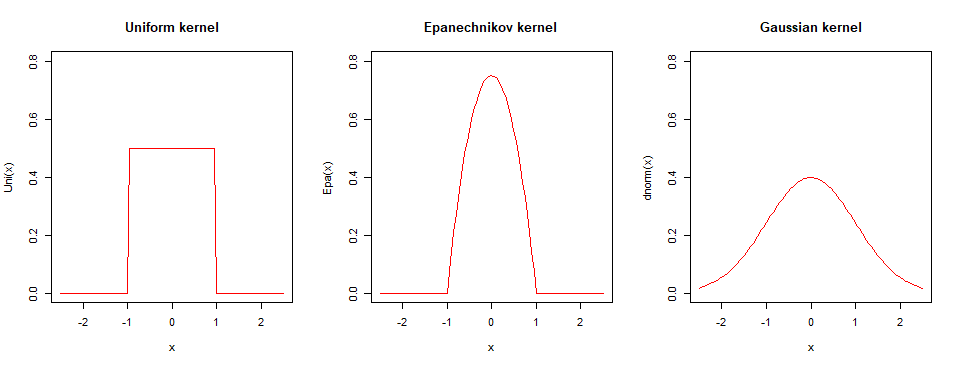
\includegraphics[width = 18cm]{kernels.png}
		\caption{Kernel density functions}\label{fig:kernels}
	\end{center}
\end{figure}

One can easily see that the local constant estimator given above is numerically equivalent to
\begin{align*}
	\hat g^{const}_n(x) = \frac{(nh)^{-1}\sum_{i = 1}^n K\left( \frac{X_i - x}{h}\right) Y_i}{(nh)^{-1}\sum_{i = 1}^n K\left( \frac{X_i - x}{h}\right)}
\end{align*}
with $K$ being the uniform kernel.
Dividing both the numerator and denominator by $nh$ is for technical convenience.
From a straightforward calculation, one can find that this $\hat g^{const}_n(x)$ is equivalent to the solution of the following weighted least squares problem:
\begin{align*}
	\hat g^{const}_n(x) = \argmin_a \sum_{i = 1}^n (Y_i - a)^2K\left( \frac{X_i - x}{h}\right).
\end{align*}
Hence, the local constant estimator can be viewed as fitting a constant-only model to the (weighted) local observations in the neighborhood of $x$ (this is why the estimator is called local ``constant'').

As an extension of the local constant approach, we can consider fitting a linear regression model to the local observations instead of simply taking the average or fitting a constant-only model.
Such an approach is called the \textbf{local linear regression\index{local linear regression}}.
That is, the local linear kernel regression estimator is defined as $\hat g^{ll}_n(x) \equiv \hat a_n$, where
\begin{align*}
	(\hat a_n, \hat b_n) = \argmin_{(a, b)} \sum_{i = 1}^n (Y_i - a - b (X_i -x))^2K\left( \frac{X_i - x}{h}\right).
\end{align*}
It is known that by including an additional regressor $(X_i - x)$, the local linear regression estimator achieves a nice bias-correction property that the local constant estimator does not have (for more details, see, e.g., \cite{li2007nonparametric}).
As a further generalization, one may consider including higher order polynomials $(X_i - x)^2$, $(X_i - x)^3$, \ldots as additional regressors.
These estimators are called the local polynomial estimators.

\begin{figure}[h!]
	\begin{center}
		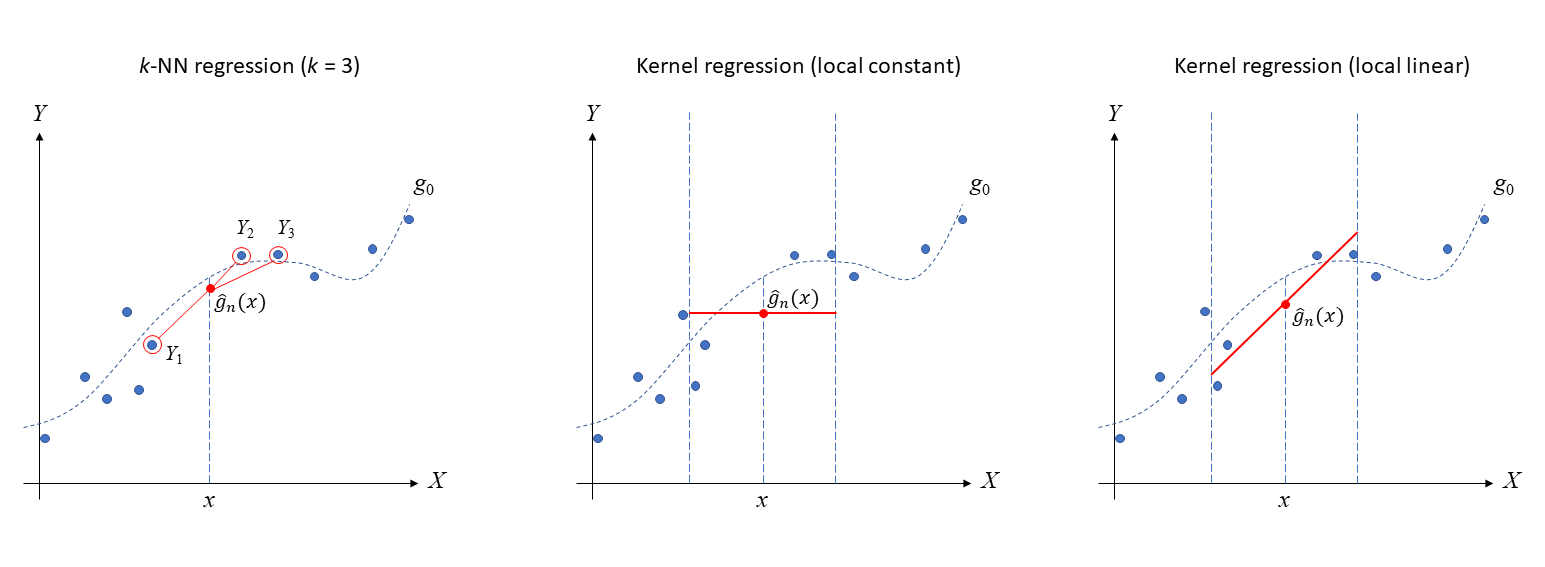
\includegraphics[width = 18cm]{localreg.png}
		\caption{Loacal nonparametric regression}
	\end{center}
\end{figure}

Here, let us provide a sketch for the proof of the consistency of $\hat g^{const}_n(x)$.
Let $f_X$ be the density function of $X$.
We first show that the numerator term of $\hat g^{const}_n(x)$ converges to $\E[Y \mid X = x]f_X(x)$ in probability.
Observe that
\begin{align*}
	\E\left[\frac{1}{nh} \sum_{i = 1}^n K\left( \frac{X_i - x}{h}\right) Y_i \right] 
	& = \frac{1}{h}\E\left[ K\left( \frac{X - x}{h}\right) Y \right] \;\; \text{(IID assumption)}\\
	& = \frac{1}{h}\int K\left( \frac{w - x}{h}\right) \E[ Y \mid X = w] f_X (w)\text{d}w \;\; \text{(LIE)} \\
	& = \int K(u) \E[ Y \mid X = x + uh] f_X (x + uh)\text{d}u \;\; \text{(change of variables: $u = (w-x)/h$)}.
\end{align*}
Recalling that $\int K(u)\text{d}u = 1$ and assuming that $\E[ Y \mid X = \cdot]$ and $f_X (\cdot)$ are bounded continuous functions, we have 
\begin{align*}
	\lim_{h \to 0} \E\left[\frac{1}{nh} \sum_{i = 1}^n K\left( \frac{X_i - x}{h}\right) Y_i \right] = \E[ Y \mid X = x] f_X (x)
\end{align*}
by the bounded convergence theorem.
By similar but slightly more tedious calculations, we can show that the variance of $(nh)^{-1} \sum_{i = 1}^n K\left( \frac{X_i - x}{h}\right) Y_i$ is of order $O((nh)^{-1})$.
Thus, if $h \to 0$ and $nh \to \infty$ as $n \to \infty$, by Chebyshev's inequality, we get $(nh)^{-1} \sum_{i = 1}^n K\left( \frac{X_i - x}{h}\right) Y_i \overset{p}{\to} \E[ Y \mid X = x] f_X (x)$.

By the same argument as above, we can prove that the denominator of $\hat g^{const}_n(x)$, $(nh)^{-1} \sum_{i = 1}^n K\left( \frac{X_i - x}{h}\right)$, converges to $f_X(x)$ in probability (this is the so-called \textbf{kernel density estimator\index{kernel density estimator}}) if $h \to 0$ and $nh \to \infty$ as $n \to \infty$.
Combining these results together, the consistency of $\hat g^{const}_n(x)$ is proved.

Note that, similar to the $k$NN regression estimator, there is a bias-variance trade-off for the choice of the bandwidth $h$.
As we have discussed, as $n$ increases, $h$ must converge to zero sufficiently slowly so that $nh$ can increase to infinity.
Intuitively, the effective sample size for a kernel regression is of order $O(nh)$ for each evaluation point, and thus to apply the law of large numbers, $nh$ must grow to infinity.

\bigskip

So far, we have focused on the case where the dimension of $X$ is just one.
When $X = (X_1, \ldots, X_d)$ is a general $d$-dimensional variable, the aforementioned estimators require some modifications.
Specifically, we introduce a ``multivariate'' kernel weighting function, say $\mbf{K}(u)$, where $u = (u_1, \ldots, u_d) \in \mathbb{R}^d$, and we can estimate $g_0(x)$ in a similar manner using $\mbf{K}(u)$ in the place of $K(u)$.
One simple way to construct $\mbf{K}(u)$ is to take the product of one-dimensional kernel functions: $\mbf{K}(u) = \prod_{j=1}^d K(u_j)$.
For example, if one employs the same bandwith $h$ for all $X_j$'s, the product uniform kernel function is
\begin{align*}
	\mbf{K}\left(\frac{X_i - x}{h}\right) = \frac{1}{2^d}\mbf{1}\{|X_{i,1} - x_1| \le h\}\mbf{1}\{|X_{i,2} - x_2| \le h\} \times \cdots \times \mbf{1}\{|X_{i,d} - x_d| \le h\}.
\end{align*}
This means that only the observations contained in the $d$-dimensional cube centered at $x$ with each side length of $2h$ can be used for estimating $g_0(x)$.
If the data are uniformly distributed on $\mcl{X}$, the size of the subsample in each cube is of order $O(nh^d)$.
Therefore, since $h$ is assumed to tend to zero, the size of the effective sample decreases ``exponentially'' (not proportionally) with respect to $d$.
Thus, nonparametric estimation of $g_0(x)$ becomes less and less feasible quickly and inefficient as $d$ grows.
This issue is known as the \textbf{curse of dimensionality\index{curse of dimensionality}}.
As far as I can see in the empirical literature, full nonparametric regression has rarely been considered when $d$ is larger than three, except when the sample size is very large (e.g., $10^5$ or more).

\subsection{Series regression}

Again, we first focus on the estimation of the model in \eqref{eq:nonpara} with a one-dimensional $X$, and extend the discussion to more general cases later.
The idea of approximating a general continuous function by a linear combination of basis functions has a long history.
Perhaps one of the most familiar to readers would be the Maclaurin expansion (i.e., the Taylor expansion at 0):
assuming that $g_0(\cdot)$ is sufficiently many times differentiable, at each $x \in \mcl{X}$
\begin{align*}
	g_0(x) = g_0(0) + g_0^{(1)}(0)x + \frac{g_0^{(2)}(0)}{2!}x^2 + \cdots + \frac{g_0^{(k)}(0)}{k!}x^k + \cdots,
\end{align*}
where $g_0^{(k)}$ denotes the $k$-th order derivative of $g_0$.
This suggests that if $g_0(\cdot)$ is sufficiently smooth, we can approximate $g_0(x)$ by $g_0(x) \approx p(x)^\top \theta_0$ with $p(x) = (1, x, x^2, \ldots, x^k)^\top$, the \textbf{power series} of order $k$, and $\theta_0 = (g_0(0), g_0^{(1)}(0), \ldots, g_0^{(k)}(0)/k!)^\top$.

A similar well-known result is the Weierstrass approximation theorem.
The theorem states that for any continuous function on a closed interval $\mcl{X}$, the same power-series approximation holds in the sense that the approximation error $g_0(x) - p(x)^\top \theta_0$ can be made arbitrarily small for any $x \in \mcl{X}$ by choosing a sufficiently large polynomial order and an appropriate coefficient vector $\theta_0$. 
Remarkably, the differentiability is not required here.

Historically, the most important series expansion result for humankind would be the \textbf{Fourier series\index{Fourier series}} expansion.
The French mathematician Joseph Fourier (1768-1830) claimed that any periodic function can be decomposed into a linear combination of sine and cosine curves.
Although its formal proof was not given by Fourier, it was later shown that his claim was after all true for a wide class of functions.
Then, named after his discovery, the following series expansion is called the Fourier series expansion: for a continuous function $g_0(\cdot)$ on a closed interval $\mcl{X}$,
\begin{align*}
	g_0(x) = a_0 + a_1\sin(\omega x) + b_1\cos(\omega x) + a_2\sin(\omega 2 x) + b_2\cos(\omega 2 x) + \cdots + a_k\sin(\omega k x) + b_k\cos(\omega k x) + \cdots,
\end{align*}
where $\omega$ is a constant determined by the size of $\mcl{X}$.

In Figure \ref{fig:seriesreg}, we provide numerical evidence for the power series approximation and the Fourier series approximation.
In the figure, the true functional form of $g_0(\cdot)$ is presented as the dotted curve.
We can clearly observe that in both series expansions, more and more precise approximation can be achieved by increasing the order of the basis functions.

\begin{figure}[h!]
	\begin{center}
		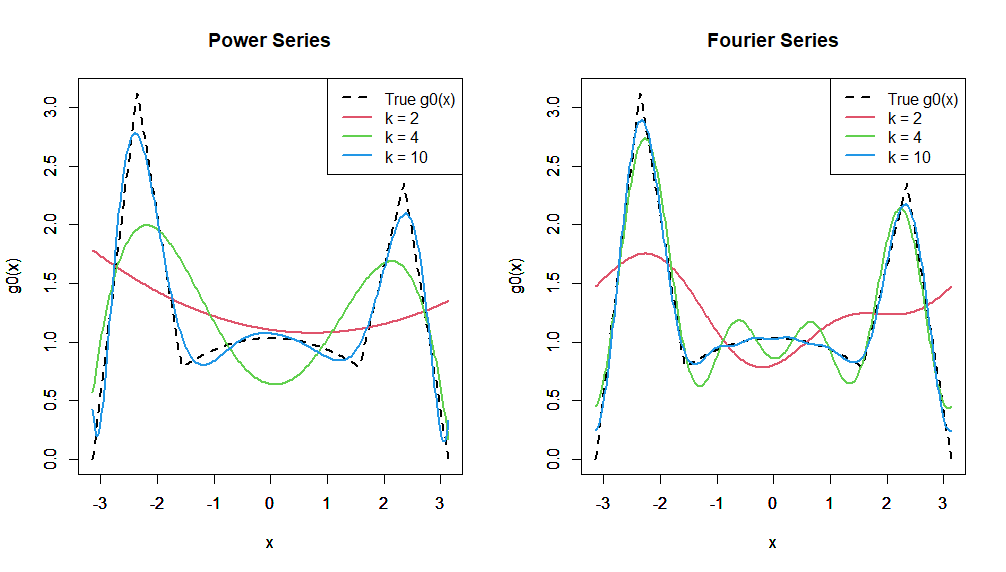
\includegraphics[width = 17cm]{seriesreg.png}
		\caption{Series approximation}\label{fig:seriesreg}
	\end{center}
\end{figure}

As such, with suitable continuity conditions, a fairly large class of functions can be approximated by some series expansion.
In addition to those introduced above, basis functions that are often adopted in applications include splines, wavelets, artificial neural networks, and so forth (see \cite{chen2007large} for their definitions and other examples).

Now, let $\{p_1(x), p_2(x), \ldots \}$ be a sequence of $\mathbb{R}$-valued basis functions, and $p(x) = (p_1(x), \ldots , p_k(x))^\top$.
We assume that for a sufficiently large $k$, there exists a $k \times 1$ vector $\theta_0$ such that the target function $g_0(\cdot)$ can be well-approximated by $p(\cdot)^\top\theta_0$ uniformly over $\mcl{X}$ in the following sense:
\begin{align*}
	|g_0(x) - p(x)^\top\theta_0 | \le O(k^{-\alpha}) \;\; \text{for any $x \in \mcl{X}$},
\end{align*}
where $\alpha > 0$ is a constant that depends on the choice of the basis function, the smoothness of $g_0$, and the dimension of $X$ (for details, see \cite{chen2007large}).
The smoother the function $g_0$ (the larger number of derivatives $g_0$ has), the larger $\alpha$ is.\footnote{
	Among the basis functions listed above, while the power series is quite popular, it is known that the power series expansion has relatively a ``slower'' convergence rate than the others.
}
Using this series approximation, we can rewrite \eqref{eq:nonpara} as follows:
\begin{align*}
	Y
	& = g_0(X) + \eps\\
	& = p(X)^\top\theta_0 + \eta
\end{align*}
where $\eta \equiv g_0(X) - p(X)^\top\theta_0 + \eps$.
Thus, the nonparametric regression model can be transformed into a ``linear regression'' model with increasing dimension.
Indeed, we can estimate $\theta_0$ simply by running an OLS regression of $Y$ on $p(X)$:\footnote{
	Here, we implicitly assume for simplicity that $\frac{1}{n}\sum_{i = 1}^n p(X_i)p(X_i)^\top$ is a nonsingular matrix.
	However, noting that the dimension of this matrix grows to infinity along with $n$, it is generally possible that the matrix is not invertible for finite $n$.
	In that case, the inverse should be replaced by a generalized inverse.
	}
\begin{align*}
	\hat \theta_n 
	& \equiv \argmin_\theta \frac{1}{n}\sum_{i = 1}^n (Y_i -  p(X_i)^\top\theta)^2 \\
	& = \left(\frac{1}{n}\sum_{i = 1}^n p(X_i)p(X_i)^\top\right)^{-1}\frac{1}{n}\sum_{i = 1}^n p(X_i)Y_i
\end{align*}
Once we obtain $\hat \theta_n$, for any given $x \in \mcl{X}$, we can estimate $g_0(x)$ by $\hat g_n(x)  \equiv p(x)^\top \hat \theta_n$.
Thus, the series regression is able to recover the shape of $g_0(\cdot)$ much more easily than the kernel regression.

To prove the consistency of $\hat g_n(x)$, by the triangle inequality, observe that
\begin{align*}
	|\hat g_n(x) - g_0(x)|
	& \le |p(x)^\top (\hat \theta_n - \theta_0)| + |g_0(x) - p(x)^\top \theta_0| \\
	& \le |p(x)^\top (\hat \theta_n - \theta_0)| + O(k^{-\alpha})
\end{align*}
Hence, it suffices to show that $|p(x)^\top (\hat \theta_n - \theta_0)| = o_P(1)$.
Here, assuming that the basis functions are bounded, we have $||p(x)|| = (p_1^2(x) + \cdots + p_k^2(x))^{1/2} = O(\sqrt{k})$.
Further, under some regularity conditions, we can show that
\begin{align}\label{eq:seriesrate}
		||\hat \theta_n - \theta_0|| = O_P\left( \sqrt{\frac{k}{n}} + k^{-\alpha}\right).
\end{align}
A sketch of the proof of this result can be found in the appendix of this chapter.
Then, combining these results with Cauchy-Schwarz inequality gives that $|p(x)^\top (\hat \theta_n - \theta_0)| \le ||p(x)|| \cdot ||\hat \theta_n - \theta_0 || = O_P(k/\sqrt{n} + k^{1/2 - \alpha})$.\footnote{
	This evaluation is actually a rough bound.
	For more sophisticated results, see, for example, \cite{belloni2015some} and \cite{chen2015optimal}.
}
Thus, if $\alpha > 1/2$ (i.e., $g_0$ is sufficiently smooth) and $k$ grows to infinity sufficiently slowly so that $k/\sqrt{n} \to 0$ is maintained, we obtain $\hat g_n(x) - g_0(x) \overset{p}{\to} 0$ for any $x \in \mcl{X}$, as desired.

\begin{comment}
To prove the asymptotic normality, we require much stronger conditions.
Here, we only state the result under the homoskedasticity assumption $\E[\eps^2 \mid X] = \sigma^2$: for a given $x \in \mcl{X}$,
\begin{align*}
	\frac{\sqrt{n}(\hat m_n(x) - g_0(x))}{\sigma \sqrt{p(x)^\top \E[p(X)p(X)^\top]^{-1}p(x)}} \overset{d}{\to} N(0,1).
\end{align*}
Then, based on this result, we can compute the confidence interval for each $g_0(x)$.
\end{comment}

\bigskip

Now we turn to the cases where $X = (X_1, \ldots, X_d)$ is a general $d$-dimensional variable.
As can be inferred from a multivariate Taylor expansion, if $X$ is $d$-dimensional, the number of basis functions required to approximate the target function increases in the order $O(k^d)$.
In general, we can construct a multivariate basis functions by taking the Kronecker product of univariate basis functions:
\begin{align*}
	p(x) = p(x_1) \otimes p(x_2) \otimes \cdots \otimes p(x_d).
\end{align*}
Thus, if $d$ is not small, the number of coefficient parameters to be estimated easily reaches several hundreds, resulting in a serious loss of efficiency.
This is the series-regression version of the curse of dimensionality.

\subsection{An empirical illustration: estimation of Engel curve}

As an empirical illustration, we nonparametrically estimate the Engel curve for food consumption using the local constant kernel regression and the series regression based on B-splines; a B-spline function is a piecewise polynomial defined by a set of ``cut points'', called \textbf{knots}.

Install \textbf{np} and \textbf{splines} packages, and load them.
The data used here is \texttt{Engel95}, a random sample taken from the U.K. Family Expenditure Survey 1995, which can be imported from the \textbf{np} package.

\begin{lstlisting}[basicstyle=\ttfamily\footnotesize, frame=single]
 library(np) # run nonparametric kernel regression
 library(splines) # compute b-spline functions

 data("Engel95") # sample size n = 1655
 food <- Engel95$food # share of food consumption
 exp  <- Engel95$logexp # log of total expenditure 
\end{lstlisting}

We first run the kernel regression using the \textbf{npreg} function.
This function automatically computes an optimal bandwidth parameter $h$, so that we do not need to specify it.

\begin{lstlisting}[basicstyle=\ttfamily\footnotesize, frame=single]
# Kernel regression #
 ghat_kernel <- npreg(food ~ exp)
\end{lstlisting}

Next, we perform the series regression.
The B-spline basis function can be computed using the \textbf{bs} function.
Here, we set the 25\%, 50\%, and 75\% empirical quantiles of \texttt{exp} as the knot values and create B-splines with $k = 6$.
After the B-splines are created, we simply run an OLS regression.

\begin{lstlisting}[basicstyle=\ttfamily\footnotesize, frame=single]
# Spline series regression #
 knots <- quantile(exp, (1:3)/4)
 p <- bs(exp, knots = knots) # compute the B-splines with k = 6
 ghat_spline <- predict(lm(food ~ p))
\end{lstlisting}

To summarize the estimation results of nonparametric regression, we present them visually.
Running the code below, we can observe that both the kernel and series regression perform very similarly.

\begin{lstlisting}[basicstyle=\ttfamily\footnotesize, frame=single]
 plot(exp, food, xlim = range(exp), ylim = range(food), 
	main = "Nonparametric regression", xlab = "exp", ylab = "food")
 par(new = T)
 plot(exp[order(exp)], ghat_kernel$mean[order(exp)], xlab = "", ylab = "",
	xlim = range(exp), ylim = range(food), type = "l", lwd = 2, col = 2)
 par(new = T)
 plot(exp[order(exp)], ghat_spline[order(exp)], xlab = "", ylab = "",
	xlim = range(exp), ylim = range(food), type = "l", lwd = 2, col = 3)
 legend("topright", c("Kernel regression", "Spline series regression"), 
	lty = c(1,1), lwd = c(2,2), col = c(2,3))
\end{lstlisting}

\begin{center}
	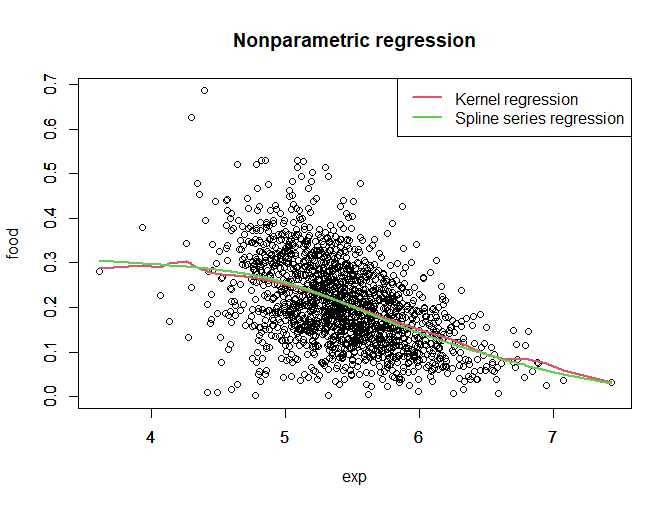
\includegraphics[width = 12cm]{engel.png}
\end{center}

\section{Semiparamtric regression}

\subsection{Partially linear models}

\subsection{Generalized additive models}

\subsection{Functional coefficient models}

\section*{Appendix: Proof of \eqref{eq:seriesrate}}

Let $\mbf{P}_n = (p(X_1), \ldots, p(X_n))^\top$, $\mbf{Y}_n = (Y_1, \ldots, Y_n)^\top$, $\mcl{E}_n = (\eps_1, \ldots, \eps_n)^\top$, $v_i \equiv g_0(X_i) - p(X_i)^\top \theta_0$, and $\mbf{V}_n = (v_1, \ldots , v_n)^\top$.
Using these notations, we can write $\mbf{Y}_n = \mbf{P}_n \theta_0 + \mbf{V}_n + \mcl{E}_n$.
Then,
\begin{align*}
	\hat \theta_n - \theta_0 
	& = \left[\mbf{P}_n^\top \mbf{P}_n /n \right]^{-1}\mbf{P}_n^\top \mbf{Y}_n /n - \theta_0 \\
	& = \left[\mbf{P}_n^\top \mbf{P}_n /n \right]^{-1}\mbf{P}_n^\top (\mbf{P}_n \theta_0 + \mbf{V}_n + \mcl{E}_n) /n - \theta_0 \\
	& = \left[\mbf{P}_n^\top \mbf{P}_n /n \right]^{-1}\mbf{P}_n^\top \mbf{V}_n /n + \left[\mbf{P}_n^\top \mbf{P}_n /n \right]^{-1}\mbf{P}_n^\top \mcl{E}_n /n 
\end{align*}
Assume that $\E[\mbf{P}_n^\top \mbf{P}_n /n]$ is positive definite for all $k$.
Applying a matrix law of large numbers to $\mbf{P}_n^\top \mbf{P}_n /n$, we have $||\mbf{P}_n^\top \mbf{P}_n /n - \E[\mbf{P}_n^\top \mbf{P}_n /n]|| = o_P(1)$.\footnote{
	A rigorous proof of this result is not that easy since $\mbf{P}_n^\top \mbf{P}_n /n$ is a matrix whose dimension increases to infinity along with $n$.
	For interested readers, see, for example, Lemma 4 of \cite{horowitz2004nonparametric}.
}
Then, with a sufficeitnly large $n$, the minimum eigenvalue of $\left[\mbf{P}_n^\top \mbf{P}_n /n \right]^{-1}$ is $O_P(1)$.
Hence, noting that the maximum eigenvalue of an idempotent matrix is at most one (see Footnote \ref{foot:idempotent}, Chapter 4),
\begin{align*}
	\left\|\left[\mbf{P}_n^\top \mbf{P}_n /n \right]^{-1}\mbf{P}_n^\top \mbf{V}_n /n \right\|^2 
	& = \mbf{V}_n^\top \mbf{P}_n \left[\mbf{P}_n^\top \mbf{P}_n /n \right]^{-2}\mbf{P}_n^\top \mbf{V}_n /n^2 \\
	& \le O_P(1) \cdot \mbf{V}_n^\top \mbf{P}_n \left[\mbf{P}_n^\top \mbf{P}_n /n \right]^{-1}\mbf{P}_n^\top \mbf{V}_n /n^2 \\
	& \le O_P(1) \cdot \mbf{V}_n^\top \mbf{V}_n /n \\
	& = O_P(1) \cdot \frac{1}{n}\sum_{i=1}^n |v_i|^2 \le O_P(k^{-2\alpha}),
\end{align*}
where in the last inequality, we have used $\max_i |v_i| = O(k^{-\alpha})$.
This implies that $\left\|\left[\mbf{P}_n^\top \mbf{P}_n /n \right]^{-1}\mbf{P}_n^\top \mbf{V} /n \right| = O(k^{-\alpha})$.

Next, note that $\E[\mcl{E}_n\mcl{E}_n^\top \mid \{X_j\}_{j=1}^n]$ is a diagonal matrix whose typical element is $\E[\eps_i^2 \mid \{X_j\}_{j=1}^n]$, which we assume to be bounded by some large constant $C$, uniformly in $i$.
Then, we have
\begin{align*}
	\E\left[ \left\| \left[\mbf{P}_n^\top \mbf{P}_n /n \right]^{-1}\mbf{P}_n^\top \mcl{E}_n /n \right\|^2 \mid \{X_j\}_{j=1}^n \right]
	& = \text{trace}\left\{ \left[\mbf{P}_n^\top \mbf{P}_n /n \right]^{-1}\mbf{P}_n^\top \E[\mcl{E}_n\mcl{E}_n^\top \mid \{X_j\}_{j=1}^n] \mbf{P}_n \left[\mbf{P}_n^\top \mbf{P}_n /n \right]^{-1}\right\}/n^2 \\
	& \le C \text{trace}\left\{ \left[\mbf{P}_n^\top \mbf{P}_n /n \right]^{-1} \right\}/n = O_P(k/n).
\end{align*}
Thus, by Markov's inequality, $\left\|\left[\mbf{P}_n^\top \mbf{P}_n /n \right]^{-1}\mbf{P}_n^\top \mcl{E}_n /n \right\|^2 = O_P(k/n)$, implying that $\left\|\left[\mbf{P}_n^\top \mbf{P}_n /n \right]^{-1}\mbf{P}_n^\top \mcl{E}_n /n \right\| = O_P(\sqrt{k/n})$.
Finally, \eqref{eq:seriesrate} holds by the triangle inequality.

%%%%%%%%%%%%%%%%%%%%%%%%%%%%%%%%%%%%%%%%
\part{Econometric Analysis of Cross-Sectional Dependence Models}
%%%%%%%%%%%%%%%%%%%%%%%%%%%%%%%%%%%%%%%%
\chapter{Cross-Sectional Dependence}
\begin{center}
	\textit{Humans are social animals} (Aristotle).
\end{center}
\section{Social interaction}
We cannot live alone away from other people.
Our behavior is inevitably affected by those around us and the social groups we belong to, and vice versa.
This interaction with others is called \textbf{social interaction\index{social interaction}}.
Thus, in order to precisely understand the nature of human behavior, such feature, i.e. social interaction, should not (or often cannot) be overlooked.

In the literature of econometrics, there is a long history in modeling the dependence structure of time series data -- the interactions between the past and present.
Estimation of econometric models with social interactions (i.e., ``cross-sectional'' interactions) is a relatively young research theme (as compared to time series literature), and now growing attention has been devoted to this field.

In an early seminal paper, \cite{manski1993identification} considered a linear social interaction model, which is called a \textbf{linear-in-means model\index{linear-in-means model}}, and distinguished three types of effects among the social interaction effects: an individual's outcome can be affected by the average outcome in the group to which he/she belongs (\textbf{endogenous effects\index{endogenous effects}}), by the average individual characteristics in the group (\textbf{contextual effects\index{contextual effect}}), and by the common environment of the group (\textbf{correlated effects\index{correlated effects}}).

For example, consider a student's academic achievement as the dependent variable of interest, say, $Y$.
Let $X$ be a determinant of academic achievement, such as whether or not belonging to an academic club.
Further, denote $e$ as the quality of class teacher.
There is an endogenous effect if individual achievement $Y$ tends to vary with the mean achievement $\bar{Y}$ of the students in the same school, class room, or other reference groups ($\bar{Y} \to Y$).
Similarly, there is a contextual effect if achievement $Y$ tends to vary with $\bar{X}$, where $\bar{X}$ is, for example, the ratio of students belonging to academic clubs ($\bar{X} \to Y$).
There are correlated effects if the students in the same class tend to achieve similarly because they are taught by the same teacher ($e \to Y$).

Importantly, the three hypotheses have different policy implications.
Consider, for example, an educational intervention providing a tutoring program to some of the students but not to the others.
If the endogenous effect exists, then an effective tutoring program not only directly helps the tutored students but, as their achievement rises, indirectly helps  other students with a feedback to further achievement gains by the tutored students.
This is the so-called \textbf{spillover effect\index{spillover effect}} or \textbf{social multiplier effect\index{social multiplier effect}}.
Exogenous effects and correlated effects do not possess such multiplier mechanism.
Thus, identification of the three social interaction effects separately is of great importance to policy implementation and evaluation.
However, as described in Chapter \ref{chap:reflection}, this is not an easy task because of the so-called \textbf{reflection problem\index{reflection problem}}.

\section{Social network}

\textbf{Social network\index{social network}} is a type of platform that facilitates social interactions between individuals.
Here, the term ``social network'' is used to refer not only to the onilne SNS (social networking service), such as Facebook or Twitter, but to the connection of individuals in a broader sense (friendship, classmates, colleagues, international trade alliance, author-coauthor relationship, etc).
Mathematically, a social network can be represented by a directed or undirected \textbf{graph}, where individuals are represented as nodes/vertices and connections between them are represented as edges of the graph.
For example, Figure \ref{fig:GATT} shows the international trade network in 1954 (\cite{arpino2017implementing}).
The black edges indicate that both countries that are connected by the edge are members of the GATT (The General Agreement on Tariffs and Trade); gray edges indicate that at least one of the two countries is not a GATT member. 

\begin{figure}[h!]
	\begin{center}
		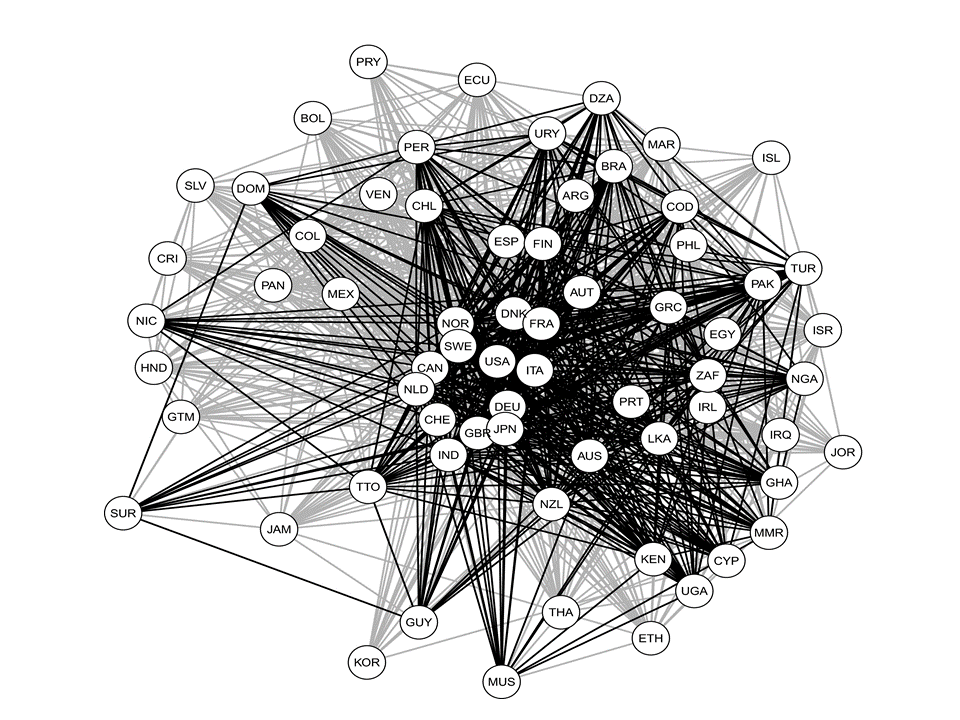
\includegraphics[width = 12cm]{GATT.png}
		\caption{Trade partners in 1954 and GATT membership, \cite{arpino2017implementing}.}
		\label{fig:GATT}
	\end{center}
\end{figure}

For another example, Figure \ref{fig:coauthor} shows the co-authorship network for 1,767 published papers in the field of statistics (\cite{said2010author}).

\begin{figure}[h!]
	\begin{center}
		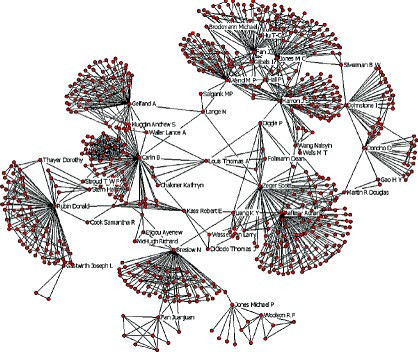
\includegraphics[width = 13cm]{coauthor.jpg}
		\caption{Co-authorship social network of statisticians, \cite{said2010author}.}
		\label{fig:coauthor}
	\end{center}
\end{figure}

Identification of linear-in-means social interaction models with network structure has been investigated by \cite{bramoulle2009identification}.
They show that, when social interactions are structured through a social network, endogenous and contextual effects can be identified (i.e., the reflection problem does not occur) on ``most'' networks.
This result will be described in detail in Chapter \ref{chap:social_network}.

\section{Spatial dependence}

Data of observations where each observation is identified by its geographical location is called spatial data. \textbf{Spatial dependence\index{spatial dependence}} (or, almost synonymously, \textbf{spatial autocorrelation\index{spatial autocorrelation}}) -- the tendency for nearby observations to be more highly correlated than those that are further apart -- distinguishes the analysis of spatial data from that of non-spatial data.
Spatial dependence is a common phenomenon observed in data from diverse areas such as climatology, geology, epidemiology, real estate market, crime, spatial price competition, etc. 

Figure \ref{fig:Tuberculosis} shows the spatial distribution of tuberculosis cases from 2002 to 2009 for each municipality in Brazil (\cite{harling2014spatial}).
In this figure, the higher rates of tuberculosis are found in the northwestern municipalities and in the coastal municipalities, indicating the presence of spatial dependence.

\begin{figure}[h!]
	\begin{center}
		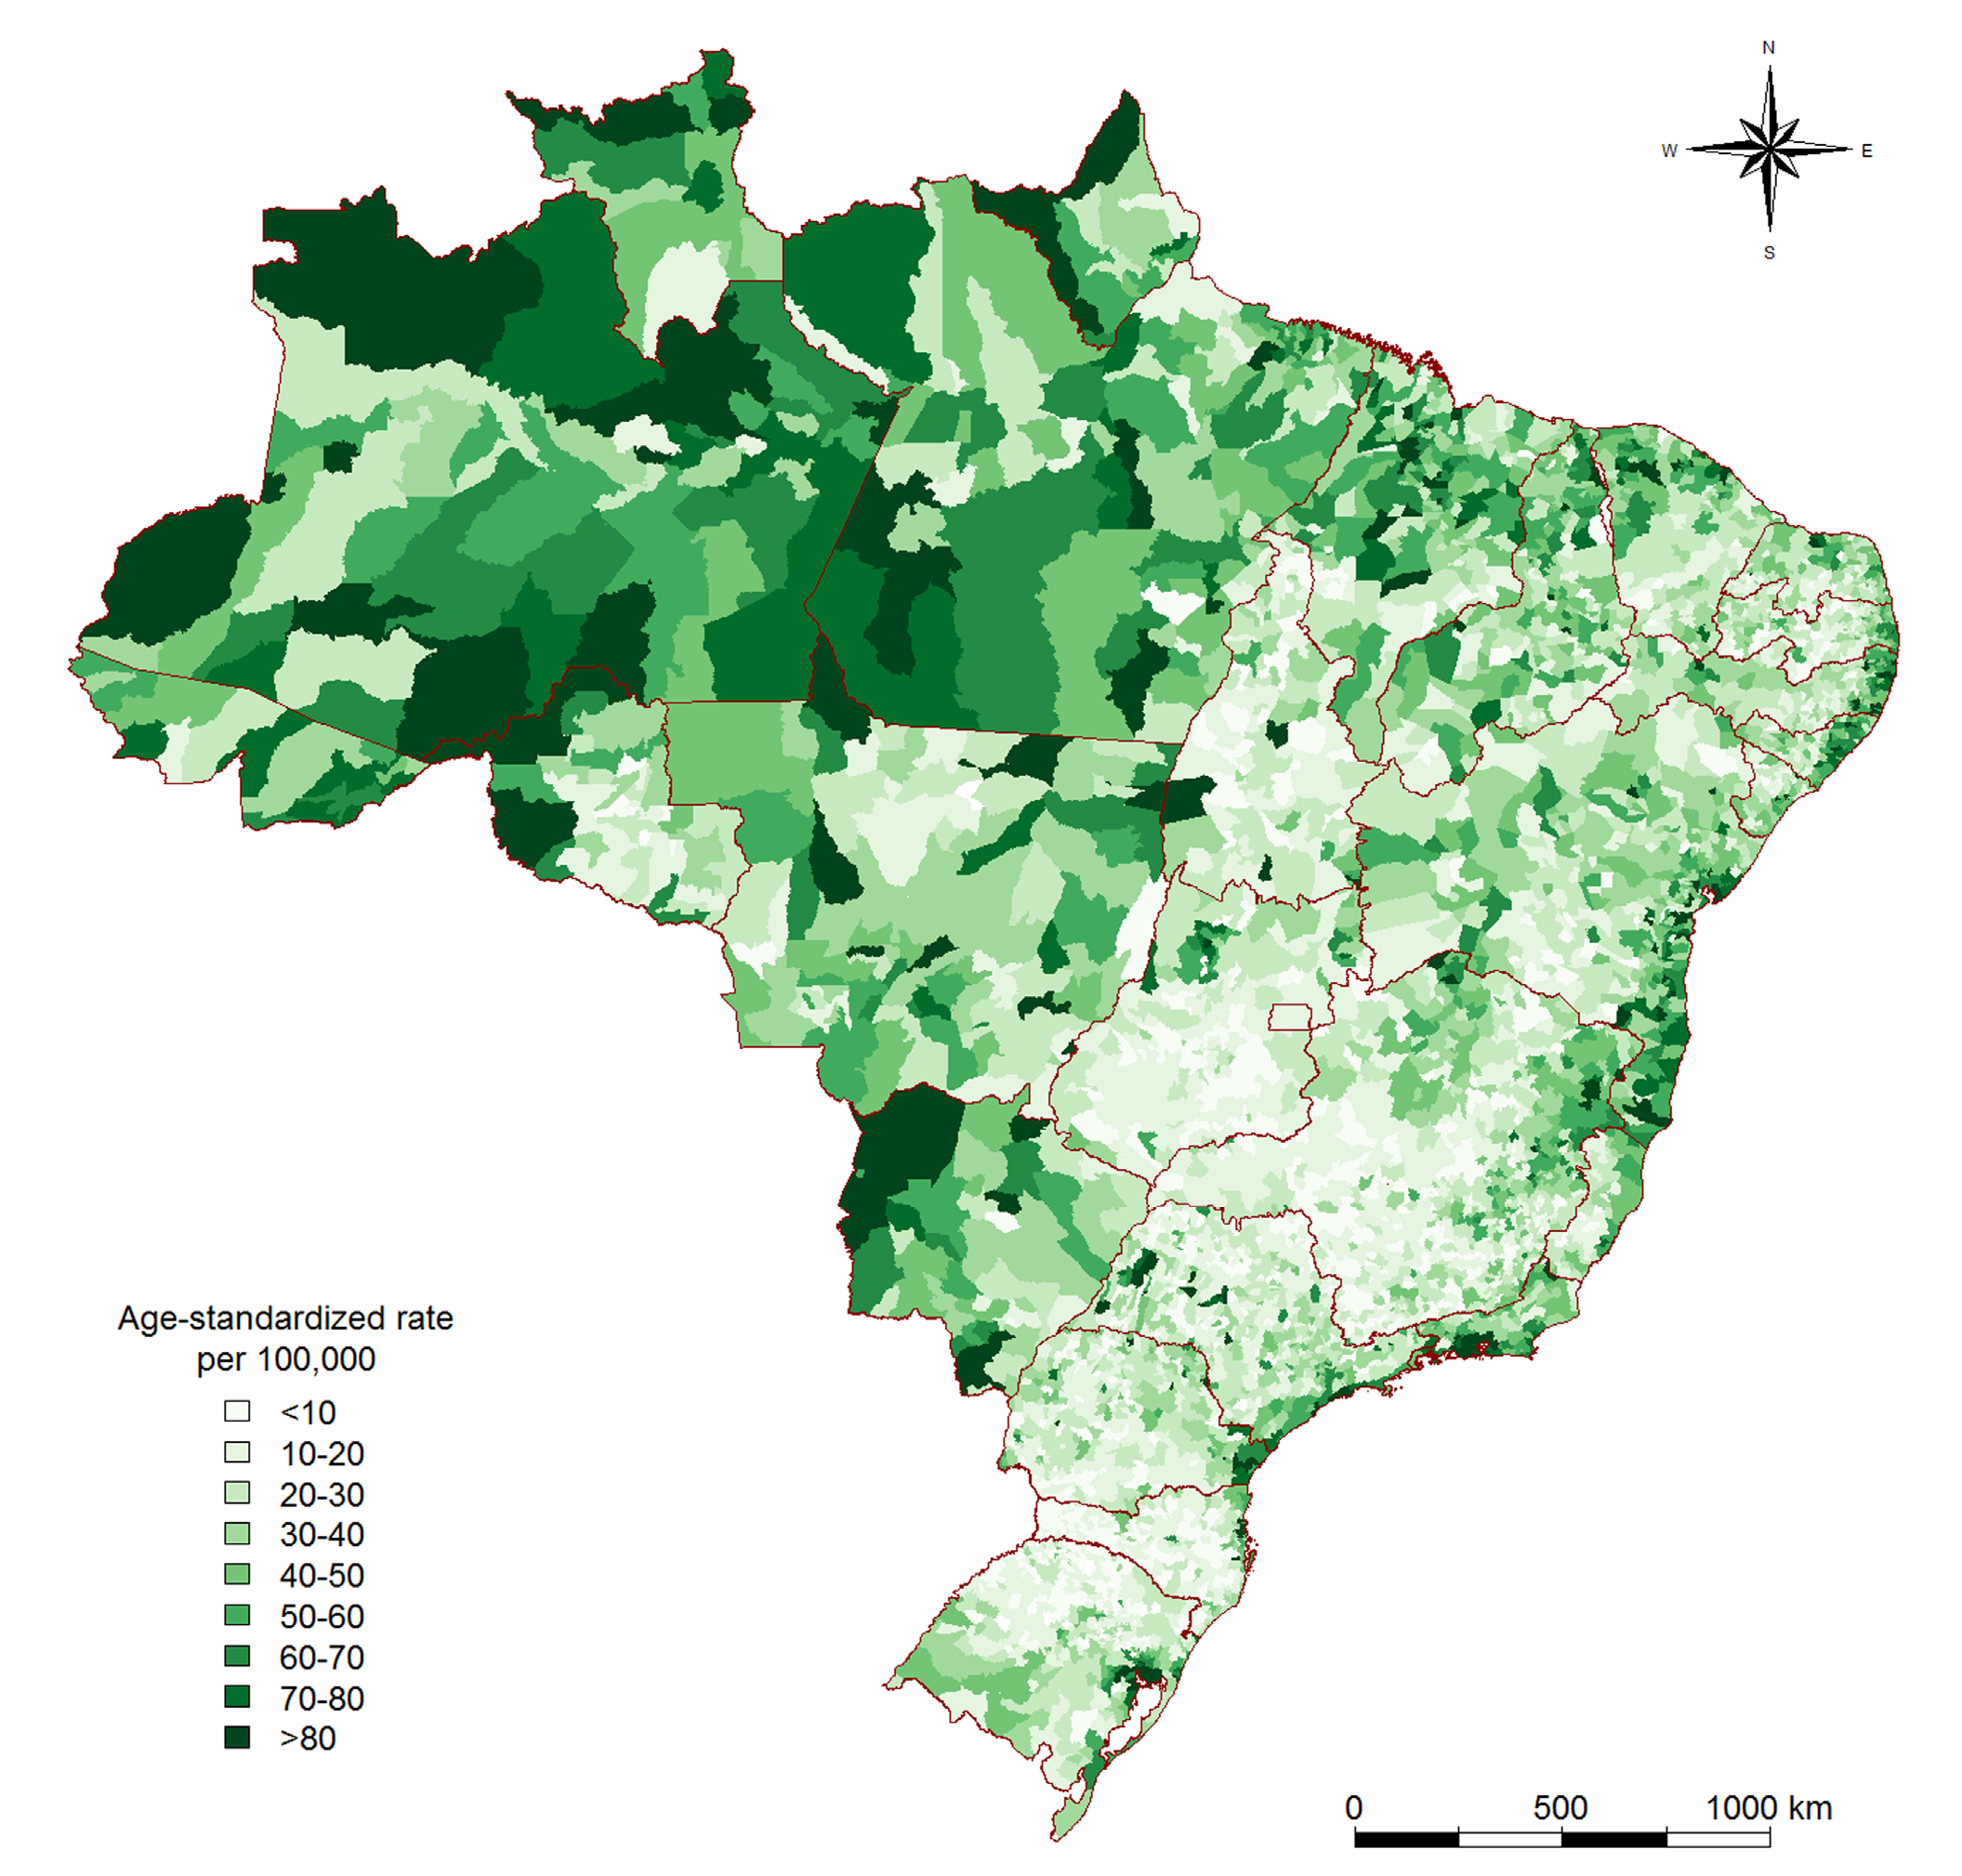
\includegraphics[width = 11cm]{Brazil.png}
		\caption{Municipal tuberculosis notification rates per 100,000 in Brazil 2002-2009, \cite{harling2014spatial}.}
		\label{fig:Tuberculosis}
	\end{center}
\end{figure}

\begin{figure}[h!]
	\begin{center}
		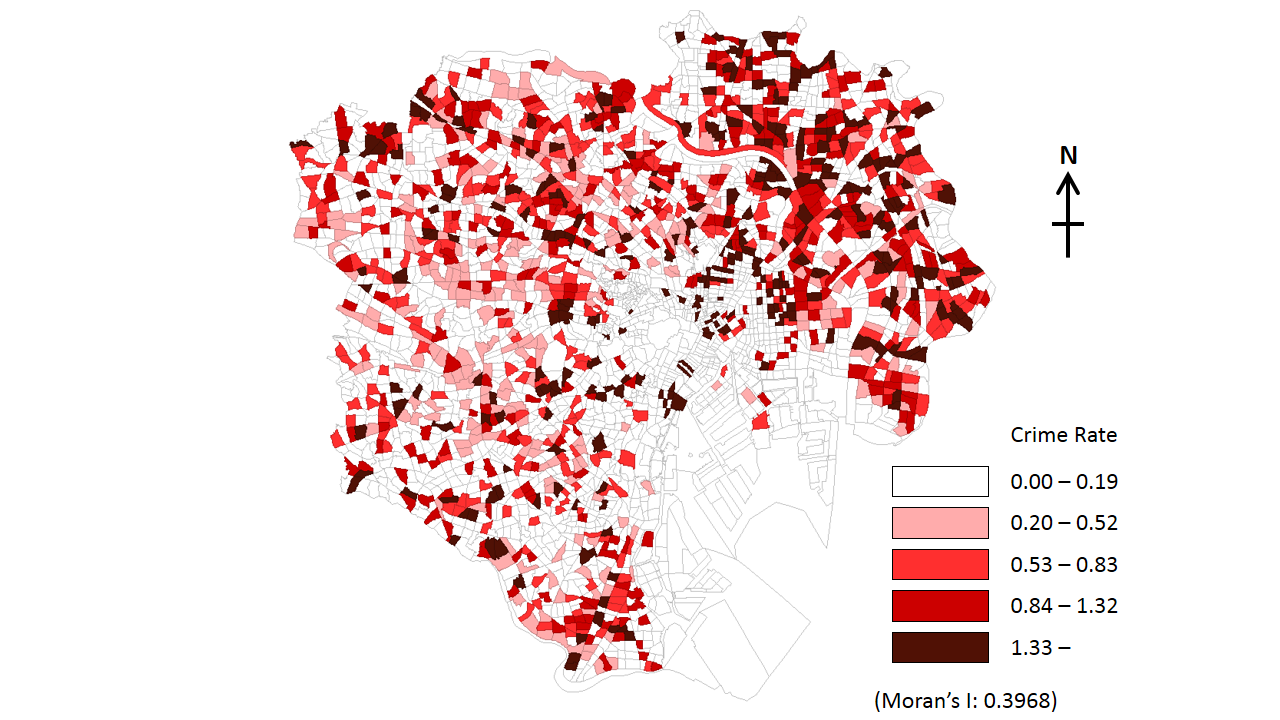
\includegraphics[width = 13cm]{crime.png}
		\caption{Distribution of household burglary rates in Tokyo 23-wards area 2011, \cite{hoshino2018semiparametric}.}
		\label{fig:crime}
	\end{center}
\end{figure}

Figure \ref{fig:crime} presents a map of Tokyo 23 wards and the value of the rate of household burglary per 1,000 households for each district in 2011 (\cite{hoshino2018semiparametric}).
The map indicates particularly low and high rates of household burglaries in the central and the northeast zones, respectively.
The \textbf{Moran's I} statistic, which is shown in the lower right of the figure (0.3968), is a type of correlation coefficient measuring the strength of spatial dependence, ranging from -1 (negative spatial dependence) to 1 (positive spatial dependence).
In Chapter \ref{chap:spatial_correlation}, we introduce several methods to statistically measure the degree of spatial correlation in data.

The field of statistics focusing on models that explicitly account for such spatial dependence is called \textbf{spatial statistics\index{spatial statistics}}, and particularly in the context of econometrics, it is called \textbf{spatial econometrics\index{spatial econometrics}}.
Since the pioneering work by \cite{anselin1988spatial}, spatial econometric methods have been widely applied in a number of empirical researches in economics.
An overview and introductory discussion of spatial econometric models are given in Chapters \ref{chap:spatial_econometrics} and \ref{chap:binary}.

One may have noticed that the spatial dependence can be seen as a special form of social interaction where the reference social group is formed based on geographical proximity.
Or, one can see social interaction as a special case of spatial dependence where the ``space'' is defined by social and economic distance between individuals.
Indeed, spatial econometric models and social interaction models have similarities in many aspects.

%%%%%%%%%%%%%%%%%%%%%%%%%%%%%%%%%%%%%%%%%%%%%%%%%%%%
%%%%%%%%%%%%%%%%%%%%%%%%%%%%%%%%%%%%%%%%%%%%%%%%%%%%
%%%%%%%%%%%%%%%%%%%%%%%%%%%%%%%%%%%%%%%%%%%%%%%%%%%%

\chapter{The Reflection Problem}\label{chap:reflection}
\section{Linear-in-means model}
\cite{manski1993identification} considered three hypotheses in order to explain the observation that individuals belonging to the same social group tend to behave similarly:
\begin{description}
	\item[Endogenous effects\index{endogenous effects}]  individuals' outcome can be affected by the mean outcome in the group.
	\item[Contextual effects\index{contextual effect}] individuals' outcome can be affected by the exogenous characteristics of the group (also referred to as \textbf{exogenous effects}).
	\item[Correlated effects\index{correlated effects}] individuals in the same group tend to behave similarly because they face similar institutional environments.
\end{description}

Let $Y$ be an outcome variable of interest (e.g., student's academic achievement), and $Z$ be a $K \times 1$ vector of individual characteristics. Also, let $X$ denote a $J \times 1$ vector of attributes characterizing an individual's reference group. Then, to account for the three distinct social effects, \cite{manski1993identification} considered the following model:
\begin{equation}\label{eq:lim1}
	Y = \alpha + \beta \E[Y \mid X] + \E[Z \mid X]^\top \gamma + Z^\top \eta + U, \quad \E[U \mid X, Z] = X^\top \delta 
\end{equation}
where $(\alpha, \beta, \gamma, \eta, \delta)$ are unknown parameters. The model in (\ref{eq:lim1}) is called the \textbf{linear-in-means model\index{linear-in-means model}}. It follows that the conditional expectation of $Y$ given $(X, Z)$ has the linear form
\begin{equation}\label{eq:lim2}
	\E[ Y \mid X, Z] = \alpha + \underbrace{\beta \E[Y \mid X]}_{\text{endogenous effect}} + \underbrace{\E[Z \mid X]^\top \gamma}_{\text{contextual effect}} + Z^\top \eta + \underbrace{X^\top \delta}_{\text{correlated effect}}
\end{equation}
If $\beta \neq 0$, $Y$ varies with $\E[Y \mid X]$, the mean of $Y$ among those individuals in the reference group characterized by $X$ (endogenous effect); if $\gamma \neq 0$, $Y$ varies with $\E[Z \mid X]$, the mean of $Z$ among those individuals in the reference group (contextual effect); and if $\delta \neq 0$, individuals in the reference group $X$ tend to behave similarly (correlated effect).

An important special case is when $X$ is a vector of indicator variables identifying which social group individuals belong to (i.e., $J$ groups in total). In this case, $\E[Y \mid X]$ and $\E[Z \mid X]$ simply denote the group means of $Y$ and $Z$, respectively, and $\delta$ represents the group-specific fixed effects.

\section{The reflection problem}

Taking the expectation of (\ref{eq:lim2}) with respect to $Z$ conditional on $X$ gives that $\E[Y \mid X]$ solves the  equation
\begin{equation}\label{eq:lim3}
	\E[Y \mid X] = \alpha + \beta \E[Y \mid X] + \E[Z \mid X]^\top (\gamma + \eta) + X^\top \delta 
\end{equation}
that is, $\E[Y \mid X]$ can be characterized as a fixed point of
\[
	H(p) \equiv \alpha + \beta p + \E[Z \mid X]^\top (\gamma + \eta) + X^\top \delta .
\]
If $\beta \neq 1$, we can solve (\ref{eq:lim3}) with respect to $\E[Y \mid X]$ as
\begin{equation}\label{eq:lim4}
	\E[Y \mid X] = \frac{\alpha}{1 -\beta} + \E[Z \mid X]^\top \frac{ (\gamma + \eta)}{1 - \beta} + X^\top \frac{\delta}{1 - \beta}. 
\end{equation}
Thus, $\E[Y \mid X]$ is a linear function of $(1, \E[Z \mid X], X)$, which implies that the endogenous effects can be expressed as the linear combination of the contextual effects and the correlated effects. Hence, in the linear-in-means model (\ref{eq:lim1}), the endogenous effects cannot be distinguished from the other two effects.

Specifically, inserting the right-hand side of (\ref{eq:lim4}) into (\ref{eq:lim2}) yields
\begin{align*}
	\E[Y \mid Z, X] 
	&= \alpha + \frac{\alpha \beta}{1 -\beta} + \E[Z \mid  X]^\top \left( \gamma +  \frac{\beta (\gamma + \eta)}{1 - \beta}\right) + Z^\top \eta  + X^\top \left( \delta + \frac{\delta \beta}{1 - \beta}\right)\\
	&= \frac{\alpha}{1 -\beta} + \E[Z \mid  X]^\top\frac{\gamma + \beta \eta}{1 - \beta} + Z^\top \eta + X^\top\frac{\delta}{1 - \beta}.
\end{align*}

\begin{theorem}[\cite{manski1993identification}]\label{thm:reflection}
Suppose that $\beta \neq 1$ and $(1, \E[Z \mid X], Z, X)$ are linearly independent.
Then, the composite parameters $(\alpha/(1 -\beta), (\gamma + \beta \eta)/(1 - \beta), \eta, \delta/(1 - \beta))$ are identified.
\end{theorem}

The interpretation of the theorem is as follows.
Suppose that a dataset $\{(Y_i, Z_i, X_i): 1 \le i \le n\}$ is available.
The theorem states that what we can estimate from the data are the four composite parameters: $\alpha/(1 -\beta)$, $(\gamma + \beta \eta)/(1 - \beta)$, $\eta$, and $\delta/(1 - \beta)$, no matter how large $n$ is.
On the other hand, the number of unknown parameters $(\alpha, \beta, \gamma, \eta, \delta)$ is five.
Therefore, we cannot identify these parameters uniquely (except for $\eta$).
In particular, the three social effects $(\beta, \gamma, \delta)$ cannot be distinguished.
This is called the \textbf{reflection problem\index{reflection problem}}.\footnote{
	Even in the presence of the reflection problem, if the value of $(\gamma + \beta \eta)/(1 - \beta)$ is non-zero, then either $\gamma$ or $\beta\eta$ (or both) is non-zero.
	Hence, one can still determine whether ``some'' social effects exist or not.
	}

If one has additional information on some parameter values, the identification result can be improved.
For example, suppose that contextual effects and correlated effects do not exist: $\gamma = \delta = 0$. Then, in this case, we have
\begin{align*}
	\E[Y \mid Z, X] = \frac{\alpha}{1 -\beta} + \E[Z \mid X]^\top\frac{\beta \eta}{1 - \beta} + Z^\top \eta .
\end{align*}
\begin{proposition}[\cite{manski1993identification}]\label{prop:reflection2} 
	Suppose that $\beta \neq 1$, $\gamma = \delta = 0$, and $(1, \E[Z \mid X], Z)$ are linearly independent. 
	Then, the composite parameters $(\alpha/(1 -\beta),  \beta \eta/(1 - \beta), \eta)$ are identified.
\end{proposition}

The proposition implies that, since $\eta$ is identified, the endogenous effect $\beta$ can be also identified from $\beta \eta / (1 - \beta)$ if $\eta \neq 0$.

\section{Numerical simulation with \R}

A direct consequence obtained from Theorem \ref{thm:reflection} and Proposition \ref{prop:reflection2} is that when $\gamma \neq 0$ the parameters of interest in model \eqref{eq:lim1}, except for $\eta$, cannot be estimated because $(1, \E[Y \mid X], \E[Z \mid X], Z)$ is linearly dependent; however, if both $\gamma$ and $\delta$ are zero, the parameters can be estimated.

We can check this result with a numerical simulation in \R.
The data-generating process used in the simulation is as follows.
\begin{lstlisting}[basicstyle=\ttfamily\footnotesize, frame=single]
N <- 300                             # sample size
X <- c(t(matrix(rnorm(10), 10, 30))) # 10 groups, 30 individuals for each.
Z <- X + X^2 + rnorm(N)              # E[Z | X] = X + X^2
U <- rnorm(N)                        # no correlated effect
 
alpha <- 1
beta  <- 0.5
gamma <- 1
eta   <- 1
 
EZ_X <- X + X^2
EY_X <- (alpha + EZ_X*(gamma + eta)) / (1 - beta)
Y    <- alpha + beta*EY_X + gamma*EZ_X + eta*Z + U
 \end{lstlisting}
The data are comprised of ten social groups with 30 members for each group, and thus, the total sample size is 300.
Here, we assume that there is no correlated effect, but the contextual effect is non-zero ($\gamma = 1$).
The conditional expectation of $Z$ given $X$ is given by $\E[Z \mid X] = X + X^2$, and that of $Y$ can be computed following equation \eqref{eq:lim4}.
Now, with this simulated dataset, if we run a linear regression of $Y$ on $(1, \E[Y \mid X], \E[Z \mid X], Z)$, ...
\begin{lstlisting}[basicstyle=\ttfamily\footnotesize, frame=single]
>  lm(Y ~ EY_X + EZ_X + Z)

Call:
lm(formula = Y ~ EY_X + EZ_X + Z)

Coefficients:
(Intercept)         EY_X         EZ_X            Z  
	 0.5158       0.7568           NA       1.0693 
\end{lstlisting}
we cannot obtain the estimate of $\gamma$ (\texttt{NA} stands for ``not available'').
If we reverse the order of $\E[Y \mid X]$ and $\E[Z \mid X], Z)$,
\begin{lstlisting}[basicstyle=\ttfamily\footnotesize, frame=single]
>  lm(Y ~ EZ_X + EY_X + Z)

Call:
lm(formula = Y ~ EZ_X + EY_X + Z)
	
Coefficients:
(Intercept)         EZ_X         EY_X            Z  
	  2.029        3.027           NA        1.069
\end{lstlisting}
now the value of $\beta$ becomes \texttt{NA}, implying that the social effects $\beta$ and $\gamma$ cannot be separately identified, i.e., the reflection problem.
However, note that the estimate of $\eta$ is unaffected by the order of regressors and is very close to its true value, that is, $\eta$ can be identified even  in the presence of the reflection problem.
This result is consistent with Theorem \ref{thm:reflection}.

Next, using the same dataset, we restrict the value of $\gamma$ to zero, as required in Proposition \ref{prop:reflection2}.
\begin{lstlisting}[basicstyle=\ttfamily\footnotesize, frame=single]
>  EY_X <- (alpha + EZ_X*eta) / (1 - beta)
>  Y    <- alpha + beta*EY_X + eta*Z + U
>  lm(Y ~ EY_X + Z)

Call:
lm(formula = Y ~ EY_X + Z)
	
Coefficients:
(Intercept)         EY_X            Z  
	 1.0022       0.5137       1.0693  
\end{lstlisting}
Then, we can estimate all parameters in the model correctly.

\section{A game theoretic interpretation}

We can interpret the linear-in-means model as a game theoretic model of incomplete information.
For simplicity, in this section we assume that contextual effects and correlated effects do not exist: $\gamma = \delta = 0$.

Let $q\in \mathbb{R}$ be an action, and the actual action made by individual $i$ is denoted by $Y_i$.
Now, assume that the payoff of individual $i$ choosing $q $ can be written as the following quadratic function:
\begin{equation*}
u_i(q, \{Y_j : X_j = X_i \})=\left[ \alpha + Z_i^\top \eta  + U_i \right] q -\frac{q^{2}}{2} + T_i(q, \{Y_j: X_j = X_i \}),
\end{equation*}
where $T_i(q, \{Y_j: X_j = X_i \})$ is a term representing the endogenous interaction between $i$ and the other members of the group to which $i$ belongs.  
For example, consider 
\begin{equation*}
T_i(q, \{Y_j : X_j = X_i \}) \equiv \dfrac{\beta}{|\{j : X_j = X_i \}|}\sum_{j : X_j = X_i}  Y_j q, \quad \beta > 0,
\end{equation*}
where $|A|$ denotes the cardinality of the set $A$.
This specification presumes that the source of social interactions is ``complementarity'': the average of group members' outcomes positively affects the individual's own marginal payoff.

Suppose that individual characteristics and error term, $Z_i$ and $U_i$, are unobservable to the other individuals including those in the same group. 
This implicitly postulates that each social group is sufficiently large such that the members of the group are not identifiable with each other.
Then, it is impossible to predict precisely the actual actions $\{Y_j: X_j = X_i \}$ from the point of view of $i$. In this situation, it is conventional to assume that each individual's behavior is characterized by a Bayesian--Nash equilibrium.
That is, a rational individual would choose an action to maximize her expected payoff:
\begin{align*}
	Y_i 
	&=\argmax_q \E_i \left[ u_i(q, \{Y_j : X_j = X_i \}) \right] \\
	&=\argmax_q \left\{ \left[ \alpha + Z_i^\top \eta  + U_i \right] q -\frac{q^{2}}{2} + \dfrac{\beta}{|\{j : X_j = X_i \}|}\sum_{j : X_j = X_i}  \E_i[Y_j] q \right\} \\
	&= \alpha + \dfrac{\beta}{|\{j : X_j = X_i \}|}\sum_{j : X_j = X_i}  \E_i[Y_j] + Z_i^\top \eta  + U_i,
\end{align*}
where $\E_i[Y_j]$ is the conditional expectation of $Y_j$ given the information set of $i$.
Notice that, because we have assumed that $Z_j$ and $U_j$ are unknown to $i$, they are not included in $i$'s information set.
Further, if $(Z, U)$'s are independent among individuals, the only available information to compute $\E_i[Y_j]$ is that $j$ is in the same group as $i$.
Consequently, we may have $\E_i[Y_j] = \E[Y | X = X_i]$; this results in the linear-in-means model:
\[
	Y_i = \alpha + \beta \E[Y | X = X_i] + Z_i^\top \eta  + U_i.
\]

The linear-in-means model assumes that an individual is affected equally by all the other members of the same group, and that she forms beliefs about their behavior utilizing only the group-level covariates.
As suggested in \cite{lee2014binary}, such framework is not appropriate for, for example, friendship networks, where the size of each social group is relatively small.
When the size of group is small, the values of the individuals characteristics $Z$ of those in the same group would be common knowledge within the members; that is $\E_i[Y_j] = \E[Y \mid Z = Z_j, X = X_i]$.
\cite{lee2014binary} called this paradigm of belief formation ``heterogeneous rational expectations''.
Heterogeneous rational expectations imply that the predicted value of the outcome of different members with different individual characteristics will be different. 
For more details, see their paper.


%%%%%%%%%%%%%%%%%%%%%%%%%%%%%%%%%%%%%%%%%%%%%%%%%


\chapter{Social Interactions through Social Networks}\label{chap:social_network}
\section{Common types of social network graphs}

\textbf{Social network\index{social network}} is a type of platform that facilitates social interactions between individuals. 
In social network analysis, networks are typically represented as \textbf{graphs\index{graph}}.
The followings are examples of social networks that we often observe in real data.
\textit{Facebook}: an undirected graph (a mutual consent is required to become Friends), \textit{Twitter}: a directed graph (a mutual consent is not required to be a Follower), \textit{married couples}: a disconnected undirected graphs, \textit{leader and followers}: a directed star graph, \textit{classroom membership}: a complete graph, and so forth.

\begin{figure}[h!]
	\begin{center}
		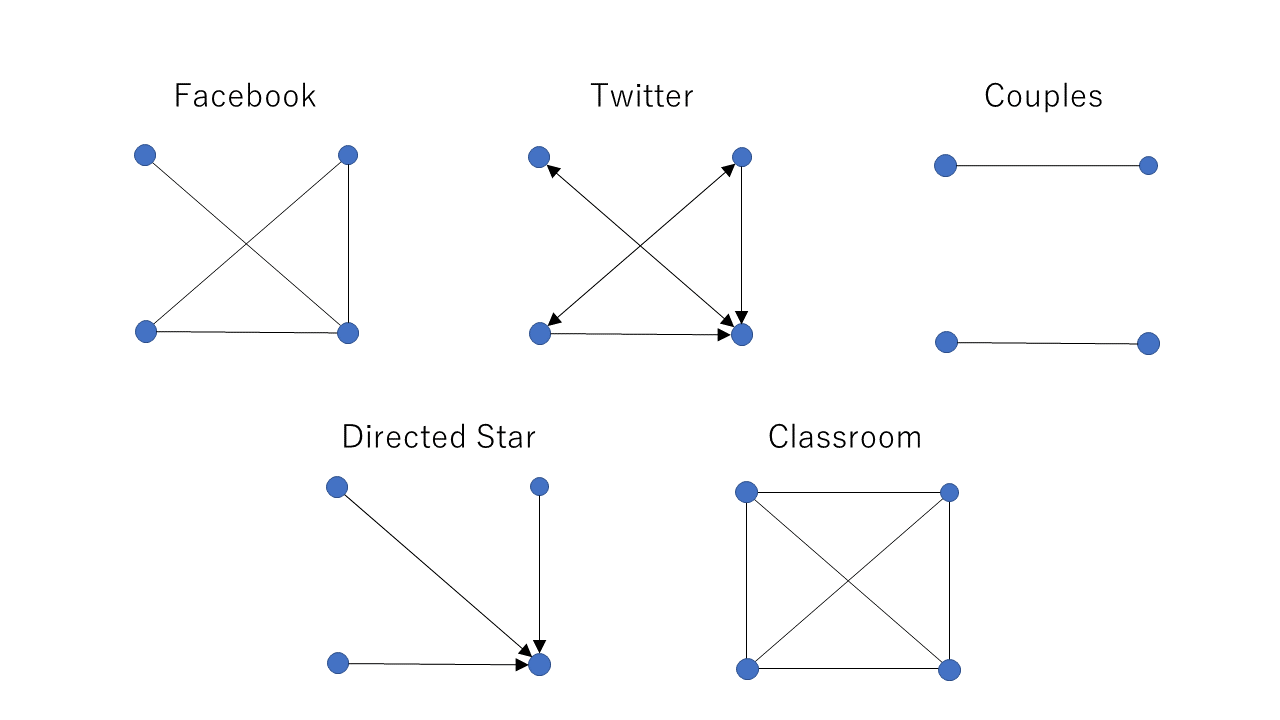
\includegraphics[width = 14cm]{snets.png}
		\caption{Social network graphs}
	\end{center}
\end{figure}

\section{Linear-in-means social network model}

When social interactions occur on social networks, such as friendship networks, the reference group for each individual is formed by the agents who are connected to her.
Thus, since the members of the reference group are distinguishable in this situation (unless the reference group is extremely large), Manski's linear-in-means model would not be appropriate.

Suppose there is a sample of $n$ individuals that form social networks.
Each individual $i$ belongs to one of these  groups, and $i$ does not necessarily interact with all the members of the group to which $i$ belongs, but may have a specific reference group (close friends) $P_i$ of size $n(i)$. 
Individual $i$ is excluded from her own reference group $P_i$, that is, $ i \not\in P_i$.
The reference is either directed  or undirected. 
For both cases, if $j$ affects $i$, we obtain $j \in P_i$.
When the friendship is directed, $j \in P_i$ does not imply the converse $i \in P_j $.
We say that an individual $i$ is \textbf{isolated\index{isolated}} if $P_i$ is empty. 
Note that while an isolated individual is not affected by the other individuals, she can still affect the others if the reference is asymmetric.
Throughout this section, we assume that not all individuals are isolated. 

\begin{figure}[h!]
	\begin{center}
	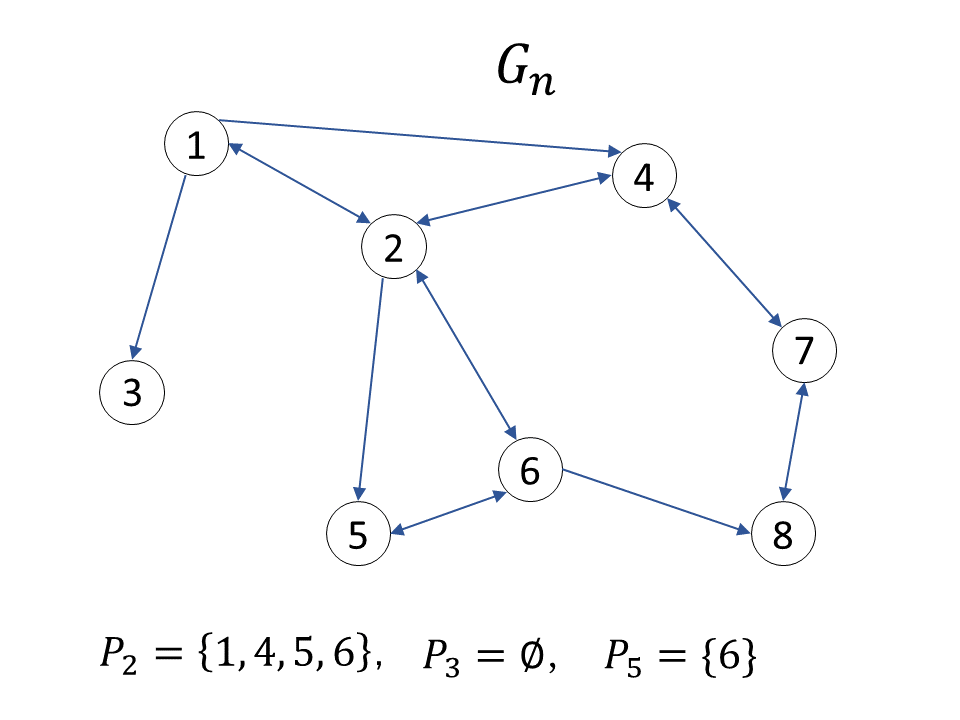
\includegraphics[width = 8cm]{reference.png}
	\caption{Reference groups. The arrows represent friendship nominations.}
	\end{center}
\end{figure}

Let $Y$ be an outcome variable of interest, and $X$ be the vector of individual characteristics. Then, we consider the following linear-in-means social network model (\cite{bramoulle2009identification}):
\begin{align}\label{eq:bramoulle}
	Y_i = \alpha + \beta \frac{\sum_{j \in P_i} Y_j}{n(i)} + X_i^\top \gamma +  \frac{\sum_{j \in P_i} X_j^\top}{n(i)} \delta + \epsilon_i, 
\end{align}
where $\beta$ captures the endogenous effect and $\delta$ the contextual effect.
For simplicity of discussion, we do not consider the correlated effects here.\footnote{
	In the linear-in-means social network models as in \eqref{eq:bramoulle}, one can account for the correlated effects by including  \textit{network fixed effects} in the model.
	For more details, see, for example, \cite{lee2007identification} and \cite{bramoulle2009identification}.
	}
The conditional expectation of $\epsilon$ given $\mathbf{X}_n = (X_1, \ldots, X_n)^\top$ is assumed to be zero: $\E[\epsilon \mid \mathbf{X}_n] = 0$ (i.e., $X$ is exogenous).

Let $\underset{n \times n}{G_n}$ be the weighted social interaction matrix (this is a directed adjacency matrix weighted by $n(i)^{-1}$).\footnote{
	Throughout this chapter, we assume that $G_n$ is non-stochastic.
	However, this assumption is indeed debatable.
	Identification and estimation of social interaction models with stochastic and endogenous $G_n$ is an important research topic in the recent literature.
}
Namely, the $(i,j)$-th element of $G_n$ is given by
\begin{align*}
	 (G_n)_{i,j} = \left\{\begin{array}{ll}
	1/n(i) & \text{ if } j \in P_i \\
	0 & \text{ otherwise }
	\end{array}\right.
\end{align*}
Note that the sum of each $i$'s row of $G_n$ is one, unless $i$ is isolated.
We can write model \eqref{eq:bramoulle} in matrix form as
\begin{align}\label{eq:bramat}
	\mbf{Y}_n = \alpha \mathbf{1}_n + \beta G_n \mbf{Y}_n + \mbf{X}_n \gamma +  G_n \mbf{X}_n \delta + \mcl{E}_n, 
\end{align}
where $\mbf{1}_n$ is an $n\times 1$ vector of ones, $\mbf{Y}_n = (Y_1, \ldots, Y_n)^\top$, and $\mcl{E}_n = (\epsilon_1, \ldots, \epsilon_n)^\top$.
Throughout the rest, we assume that $(\mathbf{1}_n, \mbf{X}_n)$ is linearly independent.

\paragraph{A game theoretic interpretation}

As opposed to Manski's linear-in-means model,  the model in \eqref{eq:bramoulle} can be seen as a game theoretic model of ``complete information''.
Assume that the payoff of individual $i$ choosing an action $q \in \mbb{R}$ can be written as the following quadratic function:
\begin{equation*}
u_i(q, \{Y_j\}_{j \in P_i})=\left[ \alpha + X_i^\top \gamma +  \frac{\sum_{j \in P_i} X_j^\top}{n(i)} \delta + \epsilon_i  \right] q -\frac{q^{2}}{2} + \beta \frac{\sum_{j \in P_i} Y_j}{n(i)} q, \;\; \beta > 0.
\end{equation*}
Here, $Y_j$'s, $j \in P_i$, are observable to $i$ under complete information. 
This specification presumes that the source of social interactions is \textbf{complementarity\index{complementarity}}: the average of friends' outcomes positively affects the individual's own marginal payoff.
Then, based on the payoff-maximization principle, the set of realized outcomes $\{Y_1, \ldots, Y_n\}$ can be characterized by a pure Nash equilibrium.
That is, 
\begin{align*}
	Y_i 
	&= \argmax_{q \in \mbb{R}}u_i(q, \{Y_j\}_{j \in P_i}) \\
	&= \alpha + \beta \frac{\sum_{j \in P_i} Y_j}{n(i)} + X_i^\top \gamma +  \frac{\sum_{j \in P_i} X_j^\top}{n(i)} \delta + \epsilon_i
\end{align*}
for all $i = 1, \ldots, n$.

For another example, one can consider
\begin{equation*}
u_i(q, \{Y_j\}_{j \in P_i})=\left[ \alpha + X_i^\top \gamma +  \frac{\sum_{j \in P_i} X_j^\top}{n(i)} \delta + \epsilon_i  \right] q -\frac{q^{2}}{2} -\frac{\beta}{2} \left( q - \dfrac{\sum_{j \in P_i} Y_j}{n(i)} \right)^2, \;\; \beta > 0.
\end{equation*}
In this case, the source of social interactions is described by \textbf{conformity\index{conformity}}: $i$'s payoff is positively affected by the degree to which she conforms with her close friends' actions. 
Solving the payoff-maximization problem, we can find that we obtain the same model as in \eqref{eq:bramoulle}.
This implies that it is generally impossible to identify the source of social interactions from model \eqref{eq:bramoulle}. 

\section{Using network structure to identify social interactions}

In the following, assume that $|\beta| < 1$.
Then, we can show that the inverse matrix $(I_n - \beta G_n)^{-1}$ exists.
For simplicity of presentation, assume that the dimension of $X$ is equal to one: $\mrm{dim}(X) = 1$.
Then, the ``reduced-form'' of model \eqref{eq:bramat} can be written as
\begin{align*}
	\mbf{Y}_n 
	& = \alpha (I_n - \beta G_n)^{-1}\mathbf{1}_n  + \gamma (I_n - \beta G_n)^{-1}\mbf{X}_n  + \delta (I_n - \beta G_n)^{-1} G_n \mbf{X}_n + (I_n - \beta G_n)^{-1}\mcl{E}_n\\
	& =  \alpha (I_n - \beta G_n)^{-1}\mathbf{1}_n  + (I_n - \beta G_n)^{-1}( \gamma I_n + \delta G_n ) \mbf{X}_n + (I_n - \beta G_n)^{-1}\mcl{E}_n.
\end{align*}
Note that it follows from the Neumann series expansion (Lemma \ref{lem:neumann}) that 
\begin{align*}
	 (I_n - \beta G_n)^{-1} 
	& = I_n + \beta G_n + \beta^2 G_n G_n + \beta^3 G_n G_n G_n + \cdots \\
	&= \sum_{t = 0}^\infty \beta^t G_n^t,
\end{align*}
where $G_n^0 = I_n$.
Thus, we have 
\[
	(I_n - \beta G_n)^{-1}\mbf{X}_n = \mbf{X}_n + \beta G_n \mbf{X}_n + \beta^2 G_n^2\mbf{X}_n + \cdots,
\]
where the first term on the right-hand side is the individual's own characteristic variables, the second term represents the average characteristics of her direct friends multiplied by $\beta$, the third term is the average characteristics of friends' friends multiplied by $\beta^2$, and so forth (see also Appendix \ref{sec:adjacency}).
This implies that, if $\beta \neq 0$, the characteristics of other individuals in the same network can affect own outcome through the social interactions, even when they are not her direct friends, and, conversely, her own characteristics affect the outcomes of the others in the same network.
In this sense, the matrix $(I_n - \beta G_n)^{-1} $ is often called the \textbf{social multiplier} matrix.

Here, assume that there are no isolated individuals.
In this case, all row-sums of $G_n^t$ for all $t = 0, 1, \ldots$ are equal to one.
Therefore, it holds that
\begin{align}\label{eq:intercept}
	\alpha  (I_n - \beta G_n)^{-1} \mathbf{1}_n 
	= \alpha \sum_{t = 0}^\infty \beta^t G_n^t \mathbf{1}_n 
	= \alpha  \sum_{t = 0}^\infty \beta^t \mathbf{1}_n  = \frac{\alpha}{1 - \beta}\mathbf{1}_n .
\end{align}
\bigskip

Now, let $\theta = (\alpha, \beta, \gamma, \delta)$ be the vector of unknown parameters to be estimated.
We say that the matrices $I_n$, $G_n$, and $G_n^2$ are linearly independent if and only if
\[
	\mu_0 I_n + \mu_1 G_n + \mu_2 G_n^2 = 0
\]
implies that $\mu_0 = \mu_1 = \mu_2 = 0$.
\begin{proposition}[\cite{bramoulle2009identification}]\label{prop:bra}
	Suppose that $\gamma \beta + \delta \neq 0$.
	
	(i)  If the matrices $I_n$, $G_n$, and $G_n^2$ are linearly independent, $\theta$  is identified.
	
	(ii) If the matrices $I_n$, $G_n$, and $G_n^2$ are linearly dependent and there are no isolated individuals, $\theta$ is not identified.
\end{proposition}

\begin{proof}
	(i) Consider two parameter vectors $\theta = (\alpha, \beta, \gamma, \delta)$ and $\theta' = (\alpha', \beta', \gamma', \delta')$.
	We show that
	\begin{align}\label{eq:ident1}
	\alpha (I_n - \beta G_n)^{-1}\mathbf{1}_n  + (I_n - \beta G_n)^{-1}( \gamma I_n + \delta G_n ) \mbf{X}_n = \alpha' (I_n - \beta' G_n)^{-1}\mathbf{1}_n  + (I_n - \beta' G_n)^{-1}( \gamma' I_n + \delta' G_n ) \mbf{X}_n
	\end{align}
	implies $\theta = \theta'$.
	Note that the above equality implies that 
	\begin{align*}
	& \alpha (I_n - \beta G_n)^{-1}\mathbf{1}_n = \alpha' (I_n - \beta' G_n)^{-1}\mathbf{1}_n\\
	& (I_n - \beta G_n)^{-1}( \gamma I_n + \delta G_n ) \mbf{X}_n = (I_n - \beta' G_n)^{-1}( \gamma' I_n + \delta' G_n ) \mbf{X}_n
	\end{align*}
	by the linear independence of $(\mbf{1}_n, \mbf{X}_n)$.
	Multiplying the both sides of the second equality by $I_n - \beta G_n$ yields
	\begin{align*}
	\gamma I_n + \delta G_n 
	& = (I_n - \beta G_n) (I_n - \beta' G_n)^{-1}( \gamma' I_n + \delta' G_n ) \\
	& = (I_n - \beta' G_n)^{-1}( \gamma' I_n + \delta' G_n )  - \beta G_n(I_n - \beta' G_n)^{-1}( \gamma' I_n + \delta' G_n ).
	\end{align*}
	Noting that $G_n(I_n - \beta' G_n)^{-1} = (I_n - \beta' G_n)^{-1} G_n$, further multiplying the both sides by $I_n - \beta' G_n$,
	\begin{align}
	& \gamma I_n + \delta G_n - \gamma \beta' G_n - \delta \beta' G_n^2 =  \gamma' I_n + \delta' G_n   - \gamma' \beta G_n   - \delta' \beta G_n^2 \nonumber \\
	& \Longrightarrow (\gamma - \gamma') I_n + (\delta - \delta' + \gamma'\beta - \gamma\beta' )G_n + (\delta'\beta - \delta\beta') G_n^2 =0. \label{eq:ident2}
	\end{align}
	Hence, we obtain $\gamma = \gamma'$, $\delta  + \gamma'\beta = \delta' + \gamma\beta'$ and $\delta'\beta = \delta\beta'$.
	Let $\lambda = \beta'/\beta$ such that $\beta' = \lambda \beta$ and $\delta' = \lambda \delta$.
	Then, 
	\begin{align*}
	\gamma = \gamma',\;\; \delta  + \gamma'\beta = \delta' + \gamma\beta' \quad 
	& \Longrightarrow\quad \delta  + \gamma \beta = \delta' + \gamma\beta' \\
	& \Longrightarrow \quad \delta  + \gamma \beta = \lambda (\delta + \gamma \beta) \\
	& \Longrightarrow \quad \lambda = 1 \quad (\because \gamma \beta + \delta \neq 0) \quad \Longrightarrow \quad \beta = \beta', \;\; \delta = \delta'.
	\end{align*}
	Finally, $\alpha = \alpha'$ follows from $\alpha (I_n - \beta G_n)^{-1}\mathbf{1}_n = \alpha' (I_n - \beta G_n)^{-1}\mathbf{1}_n$.
	
	(ii) When the matrices $I_n$, $G_n$, and $G_n^2$ are linearly dependent, we can find $\theta' = (\alpha', \beta', \gamma', \delta')$ that satisfy \eqref{eq:ident1} and \eqref{eq:ident2} but at least one of the following inequalities holds:
	\[
	\gamma - \gamma' \neq 0, \;\; \delta - \delta' + \gamma'\beta - \gamma\beta' \neq 0, \;\; \delta'\beta - \delta\beta' \neq 0.
	\]
	This implies that at least $\beta$ and $\delta$ cannot be separately identified.
	For the identification of $\alpha$, because no individual is isolated,
	\[
	\alpha (I_n - \beta G_n)^{-1}\mathbf{1}_n = \alpha' (I_n - \beta' G_n)^{-1}\mathbf{1}_n \iff \alpha/(1 - \beta) = \alpha'/(1 - \beta')
	\]
	by \eqref{eq:intercept}.
	Since $\beta$ is not identified, $\alpha$ is also not identified.
\end{proof}
\bigskip

In Proposition \ref{prop:bra}, we have assumed that $\gamma \beta + \delta \neq 0$.
The role of this assumption should be clear from the following equality.
Noting that $(I_n - \beta G_n)^{-1} = I_n +  \beta G_n(I_n - \beta G_n)^{-1}$, if $\gamma \beta + \delta = 0$, we have
\begin{align*}
	\E[\mbf{Y}_n \mid \mbf{X}_n] 
	& = \alpha (I_n - \beta G_n)^{-1}\mathbf{1}_n + \gamma (I_n - \beta G_n)^{-1}\mbf{X}_n + \delta (I_n - \beta G_n)^{-1}G_n \mbf{X}_n\\
	& = \alpha (I_n - \beta G_n)^{-1}\mathbf{1}_n + \mbf{X}_n \gamma +  (\gamma \beta + \delta) (I_n - \beta G_n)^{-1}G_n \mbf{X}_n \\
	& = \alpha (I_n - \beta G_n)^{-1}\mathbf{1}_n + \mbf{X}_n \gamma.
\end{align*}
Thus, the contextual effect vanishes when $\gamma \beta + \delta = 0$.
\bigskip

The next result shows that if $\E[G_n \mbf{Y}_n \mid \mbf{X}_n]$ is a linear function of $(\mbf{1}_n, \mbf{X}_n, G_n\mbf{X}_n)$, the matrices $I_n$, $G_n$, and $G_n^2$ become linearly dependent, and thus $\theta$ is not identified.
This result corresponds to the reflection problem of Manski's model (recall equation \eqref{eq:lim4} and Theorem \ref{thm:reflection}).
\begin{proposition}[\cite{bramoulle2009identification}]
	Suppose that $\gamma \beta + \delta \neq 0$ and that no individuals are isolated.
	If there are $(\lambda_0, \lambda_1, \lambda_2)$ satisfying $\E[G_n \mbf{Y}_n \mid \mbf{X}_n] = \lambda_0\mbf{1}_n + \lambda_1\mbf{X}_n + \lambda_2 G_n \mbf{X}_n$ for any $\mbf{X}_n$, then $I_n$, $G_n$ and $G_n^2$ are linearly dependent.
\end{proposition}

\begin{proof}
	First, by assumption
	\begin{align*}
		\E[G_n \mbf{Y}_n \mid \mbf{X}_n] 
		& = \alpha/(1 - \beta) \mathbf{1}_n  + (I_n - \beta G_n)^{-1}( \gamma G_n + \delta G_n^2 ) \mbf{X}_n\\
		& =  \lambda_0\mbf{1}_n + \lambda_1\mbf{X}_n + \lambda_2 G_n \mbf{X}_n
	\end{align*}
	for any $\mbf{X}_n$.
	This implies that $\lambda_0 = \alpha/(1 - \beta)$ and $(I_n - \beta G_n)^{-1}( \gamma G_n + \delta G_n^2 ) = \lambda_1 I_n + \lambda_2 G_n$.
	For the second equality, by multiplying the both sides by $I_n - \beta G_n$ yields
	\begin{align*}
		& \gamma G_n + \delta G_n^2  = \lambda_1 I_n + \lambda_2 G_n -  \beta \lambda_1 G_n - \beta \lambda_2 G_n^2 \\
		& \Longrightarrow \lambda_1 I_n + (\lambda_2 - \beta \lambda_1 - \gamma) G_n - (\beta \lambda_2 + \delta) G_n^2 = 0.
	\end{align*}
	Here assume that $I_n$, $G_n$, and $G_n^2$ are linearly independent.
	Then, it must hold that $\lambda_1 = 0$ and $\lambda_2 = \gamma$, and hence $\gamma \beta + \delta = 0$.
	This is a contradiction with the assumption that $\gamma \beta + \delta \neq 0$.
	Therefore, $I_n$, $G_n$, and $G_n^2$ are linearly dependent.
\end{proof}

\begin{example}[Classroom interaction: single classroom]\upshape
	Consider a school classroom of size $n$, where each student is interacted with all the other $n-1$ students in the same classroom.
	In this case, the social interaction matrix $G_n$ is characterized by a weighted complete graph with the weights being all equal to $1/(n - 1)$.
	A typical element of $G_n^2$ is given by
	\begin{align*}
		(G_n^2)_{i,j} = \left\{\begin{array}{ll}
		\sum_{k = 1} ^n (G_n)_{i,k} (G_n)_{k,j} = (n - 2)/(n-1)^2& \text{ if $i \neq j$} \\
		\sum_{k = 1} ^n (G_n)_{i,k} (G_n)_{k,j} = 1/(n-1)& \text{ if $i = j$}
		\end{array}\right.
	\end{align*}
	Therefore, we have
	\[
	\frac{1}{n - 1} I_n + \frac{n-2}{n-1} G_n = G_n^2,
	\]
	and thus $\theta$ cannot be identified.
\end{example}

\begin{example}[Classroom interaction: multiple classrooms]\upshape
	Now assume that (without loss of generality) there are two classrooms of sizes $n_1$ and $n_2$.
	In this case, the social interaction matrix $G_n$ is a block-diagonal matrix
	\[
		G_n = \left( \begin{array}{cc}
		G_{n1} & 0 \\
		0 & G_{n2}		
		\end{array}\right),
	\]
	where each $G_{nj}$ is a weighted complete graph with weights equal to $1/(n_j - 1)$, for $j = 1,2$.
	By the same argument as above, we can see that
	\[
	G^2_n = \left( \begin{array}{cc}
	\frac{1}{n_1 - 1} I_{n_1} + \frac{n_1 - 2}{n_1 - 1} G_{n1} & 0 \\
	0 & 	\frac{1}{n_2 - 1} I_{n_2} + \frac{n_2 - 2}{n_2 - 1} G_{n2}
	\end{array}\right) .
	\]
	Therefore, if $n_1 \neq n_2$, we can identify $\theta$.
	In words, the variations in classroom sizes have identification power; see \cite{lee2007identification}.
\end{example}

\begin{example}[Intransitive network]\upshape
	Suppose now that individuals interact through a network. 
	In  addition, suppose that we can find an \textbf{intransitive triad\index{intransitive triad}} (i.e., a friend of my friend is not necessarily my friend) in the network.
	For example, suppose that there is a set of three individuals $(i, j, k)$ satisfying $(G_n)_{i,j} > 0$, $(G_n)_{j,k} > 0$, but $(G_n)_{i,k} = 0$, such that the shortest path between $i$ and $k$ is of length 2.
	In this case, the $(i, k)$-th element of $G_n^2$ is larger than zero, while that of $G_n$ is zero (and of course that of $I_n$ is also zero).
	Therefore, the presence of the intransitive triad guarantees the linear independence.
	\begin{figure}[h!]
	\begin{center}
		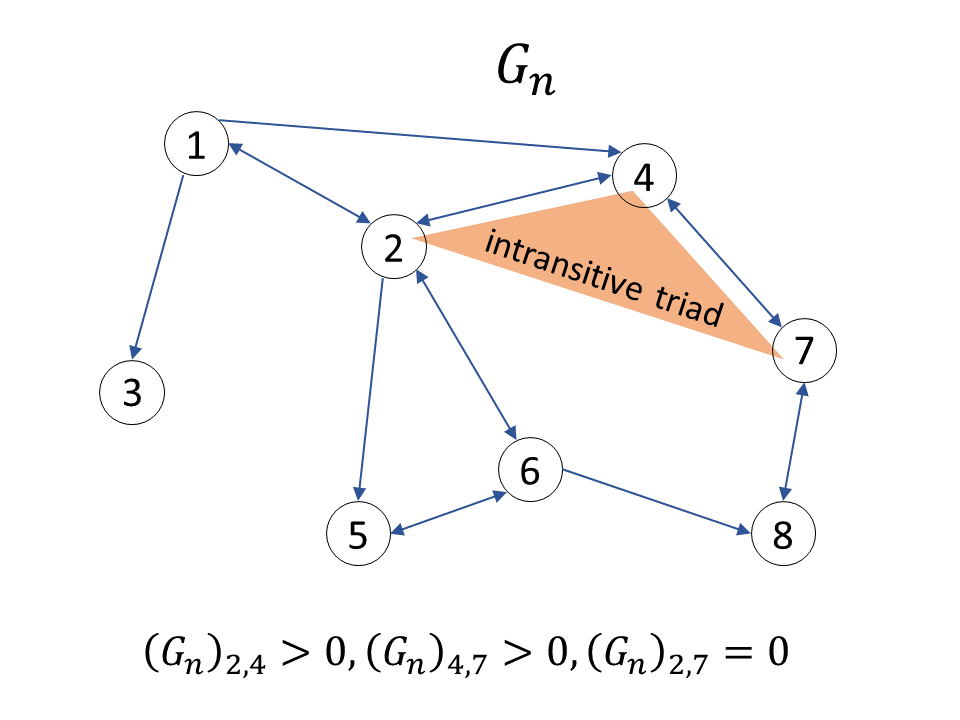
\includegraphics[width = 9cm]{intransitive.png}
		\caption{Intransitive triad}
	\end{center}
	\end{figure}
\end{example}

\hrulefill
\begin{exercise}\upshape
	Prove that if $|\beta| < 1$ the matrix $I_n - \beta G_n$ is nonsingular. (Hint: use Lemma \ref{lem:neumann})
\end{exercise}
\begin{exercise}\upshape
Prove that all row-sums of $G_n^t$ for all $t = 0, 1, \ldots$ are one when there are no isolated individuals.
\end{exercise}


\section{Estimation}\label{sec:estimation_soc}

Let us recall that the model to be estimated is \eqref{eq:bramat}:
\[
	\mbf{Y}_n = \alpha_0 \mathbf{1}_n + \beta_0 G_n \mbf{Y}_n + \mbf{X}_n \gamma_0 +  G_n \mbf{X}_n \delta_0 + \mcl{E}_n,
\]
where $\theta_0$ is the true parameter value of $\theta = (\alpha, \beta, \gamma, \delta)$.
Given the identification results as above, we here provide an approach to estimate $\theta_0$
In this section, we do not restrict the dimension of $X$ to be one.

First of all, it should be clear that the OLS estimator that simply regresses $\mbf{Y}_n$ on $(\mathbf{1}_n, G_n \mbf{Y}_n, \mbf{X}_n, G_n \mbf{X}_n)$ is inconsistent because of the endogeneity of $G_n \mbf{Y}_n$; if $i$ and $j$ are friends such that $i \in P_j$,
\begin{align*}
	\E[Y_j \epsilon_i]
	& = \E\left[\left(\alpha +\frac{\beta_0}{ n(j)} \sum_{k \in P_j} Y_k + X_j^\top \gamma_0 + \frac{1}{n(j)} \sum_{k \in P_j} X_k^\top \delta_0 + \epsilon_j\right) \epsilon_i\right] \\
	& = \frac{\beta_0}{ n(j)} \underbrace{\E\left[ \sum_{k \in P_j} Y_k \epsilon_i\right]}_{\neq \: 0} + \E[\epsilon_j \epsilon_i ].
\end{align*}
Thus, even when $\epsilon_i$ and $\epsilon_j$ are uncorrelated, unless $\beta_0 = 0$, $\E[Y_j \epsilon_i] \neq 0$ in general.

To account for this endogeneity problem, we can use a 2SLS estimator with instrumental variables.
Fortunately, a set of reasonable instrumental variables for $G_n\mbf{Y}_n$ can be easily found.
Observe that
\[
	G_n \mbf{Y}_n = \alpha_0 G_n \mathbf{1}_n + \beta_0 G^2_n \mbf{Y}_n + G_n \mbf{X}_n \gamma_0 +  G^2_n \mbf{X}_n \delta_0 + G_n \mcl{E}_n.
\]
This expression implies that $G^2_n \mbf{X}_n$ is a valid instrument for $G_n\mbf{Y}_n$, which is not included in the outcome equation \eqref{eq:bramat}, and is correlated with $G_n\mbf{Y}_n$ (assuming that $\delta_0 \neq 0$) but not with $\mcl{E}_n$.\footnote{
	Note that if the matrices $I_n$, $G_n$, and $G_n^2$ are linearly dependent, $G^2_n \mbf{X}_n$ is perfectly collinear with $(\mbf{X}_n, G_n\mbf{X}_n)$, and thus $G^2_n \mbf{X}_n$ cannot be used as an identifying instrument.
	From this, one can view the identification condition in Proposition \ref{prop:bra} that $I_n$, $G_n$, and $G_n^2$ are linearly independent as a condition ensuring that $G^2_n \mbf{X}_n$ becomes a valid instrument for $G_n\mbf{Y}_n$.
}

The 2SLS estimation procedure is as follows.
First, run a least squares regression of $G_n \mbf{Y}_n$ on $\mbf{Z}_n = (\mbf{1}_n, \mbf{X}_n, G_n\mbf{X}_n, G_n^2\mbf{X}_n)$, and compute the predicted value of $G_n\mbf{Y}_n$, say $\hat{G_n\mbf{Y}_n}$, by
\[
\hat{G_n\mbf{Y}_n} = \mbf{Z}_n(\mbf{Z}_n^\top \mbf{Z}_n)^{-1}\mbf{Z}_n^\top G_n \mbf{Y}_n.
\]
In the second stage,  run a least squares regression of $\mbf{Y}_n$ on $(\mbf{1}_n, \hat{G_n\mbf{Y}_n}, \mbf{X}_n, G_n\mbf{X}_n)$ to obtain the estimator $\hat \theta_n$ of $\theta$.
Note that since $(\mbf{1}_n, \mbf{X}_n, G_n\mbf{X}_n)$ is a subset of $\mbf{Z}_n$, it holds that $(\mbf{1}_n, \mbf{X}_n, G_n\mbf{X}_n) = \mbf{Z}_n(\mbf{Z}_n^\top \mbf{Z}_n)^{-1}\mbf{Z}_n^\top (\mbf{1}_n, \mbf{X}_n, G_n\mbf{X}_n)$, and the second-stage regression is numerically equivalent to regressing $\mbf{Y}_n$ on $\mbf{Z}_n(\mbf{Z}_n^\top \mbf{Z}_n)^{-1}\mbf{Z}_n^\top \mbf{H}_n$, where $\mbf{H}_n = (\mbf{1}_n, G_n\mbf{Y}_n, \mbf{X}_n, G_n\mbf{X}_n)$.
Hence, the 2SLS estimator $\hat \theta_n$ can be obtained actually in one step by
\begin{align}\label{eq:2slssoc}
\hat \theta_n = \left[\mbf{H}_n^\top \mbf{Z}_n(\mbf{Z}_n^\top \mbf{Z}_n)^{-1}\mbf{Z}_n^\top \mbf{H}_n  \right]^{-1}\mbf{H}_n^\top \mbf{Z}_n(\mbf{Z}_n^\top \mbf{Z}_n)^{-1}\mbf{Z}_n^\top\mbf{Y}_n.
\end{align}
Under some regularity conditions, the 2SLS estimator $\hat \theta_n$ is consistent for $\theta_0$ and asymptotically normally distributed at $\sqrt{n}$ rate; see Section \ref{sec:2slsAsymptotics}.

%%%%%%%%%%%%%%%%%%%%%%%%%%%%%%%%%%%%%%%%%%%%%%%%%
%%%%%%%%%%%%%%%%%%%%%%%%%%%%%%%%%%%%%%%%%%%%%%%%%
%%%%%%%%%%%%%%%%%%%%%%%%%%%%%%%%%%%%%%%%%%%%%%%%%

\chapter{Spatial Data}\label{chap:spatial_correlation}

\section{Spatial data}

\textbf{Spatial data\index{spatial data}} are data that are related to geographic information as part of that data. 
Geographic information refers to all kind of data that identify the spatial location of each data unit, which is stored not only in the form of point data (i.e., longitude and latitude), but also in the form of spatial polygon data (e.g., regions, districts, and municipalities) and mesh data (e.g., the distribution of air pollutants, satellite images, and brain images).
\begin{figure}[h!]
	\begin{center}
		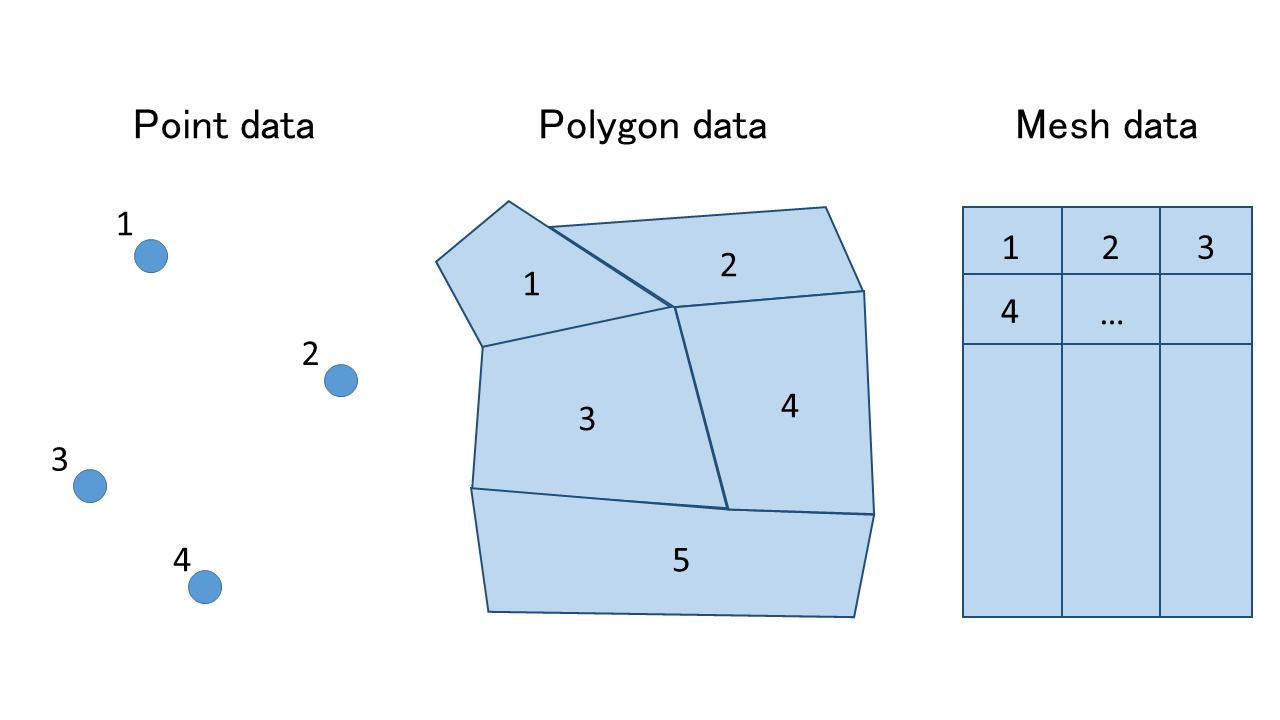
\includegraphics[width = 12cm]{spdata.png}
		\caption{Spatial data\label{fig:spdata}}
	\end{center}
\end{figure}

An integrated computational system, which is designed to store, manipulate, and visualize spatial data, is called \textbf{GIS\index{GIS}} (geographic information system). 
 The world's most popular GIS software is ArcGIS (ESRI).
 In these days, free and open source GIS softwares, such as QGIS and Grass GIS, have been becoming more popular.  
The statistical software \textbf{R} is also able to process and analyze spatial information with additional packages (such as \textbf{sf}, \textbf{spdep}, etc).

\begin{figure}[h!]
	\begin{center}
		
\includegraphics[width = 12cm]{GIS.png}
		\caption{Open-source free GIS\label{fig:GIS}}
	\end{center}
\end{figure}

\section{Moran's I and Geary's C}

\subsection{Spatial weight matrix}

The first step in any spatial data analysis is to plot the data on a map to find out if there is a specific correlational pattern in the data.
Figure \ref{fig:Tuberculosis} and \ref{fig:crime} are examples of plotted spatial data (polygon data).
In these examples, we can find a tendency that districts of similar values are spatially clustered.
This phenomenon is called \textbf{spatial autocorrelation\index{spatial autocorrelation}}, more precisely speaking, a ``positive'' spatial autocorrelation.
Negative spatial autocorrelation means that nearby districts have dissimilar values.
Although negative spatial autocorrelation is rarely observed in real data, a spatial competition under strategic substitutes potentially may generate a negative correlation (e.g., where to open convenience stores).
\begin{figure}[h!]
	\begin{center}
		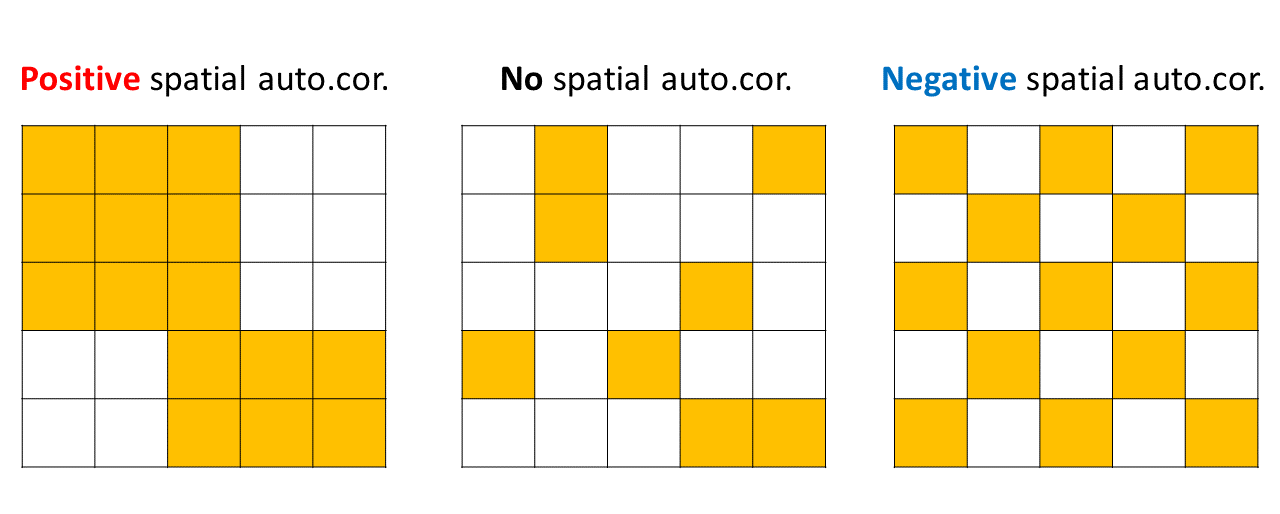
\includegraphics[width = 12cm]{spauto.png}
		\caption{Spatial autocorrelation}
	\end{center}
\end{figure}

The main objectives of spatial data analysis are to quantify and to analyze the mechanism of spatial autocorrelation in the data. 
In measuring the degree of spatial autocorrelation, one thing that needs clarification is what ``nearby'' means.
How to measure the proximity between two spatial units depends on the form of spatial data.
For point data, the proximity can be defined simply by the Euclidean distance (or, possibly other distance measures, such as road distance and travel time).
For polygon data, the proximity is often determined by whether the units share a common border or not.
For this type of proximity measure, there are two common approaches: \textbf{Rook contiguity\index{Rook contiguity}} and \textbf{Queen contiguity\index{Queen contiguity}} (based on the movement of chess pieces).
The rook contiguity defines neighbors by the existence of a common edge between two spatial units, and the queen contiguity is based on the existence of either a common edge or vertex between them (see Figure \ref{fig:contiguity}).
Note that, if one specifies a representative point of each polygon (e.g., location of administrative office, center of gravity), the distance-based proximity can be used for polygon data as well.

\begin{figure}[h!]
	\begin{center}
		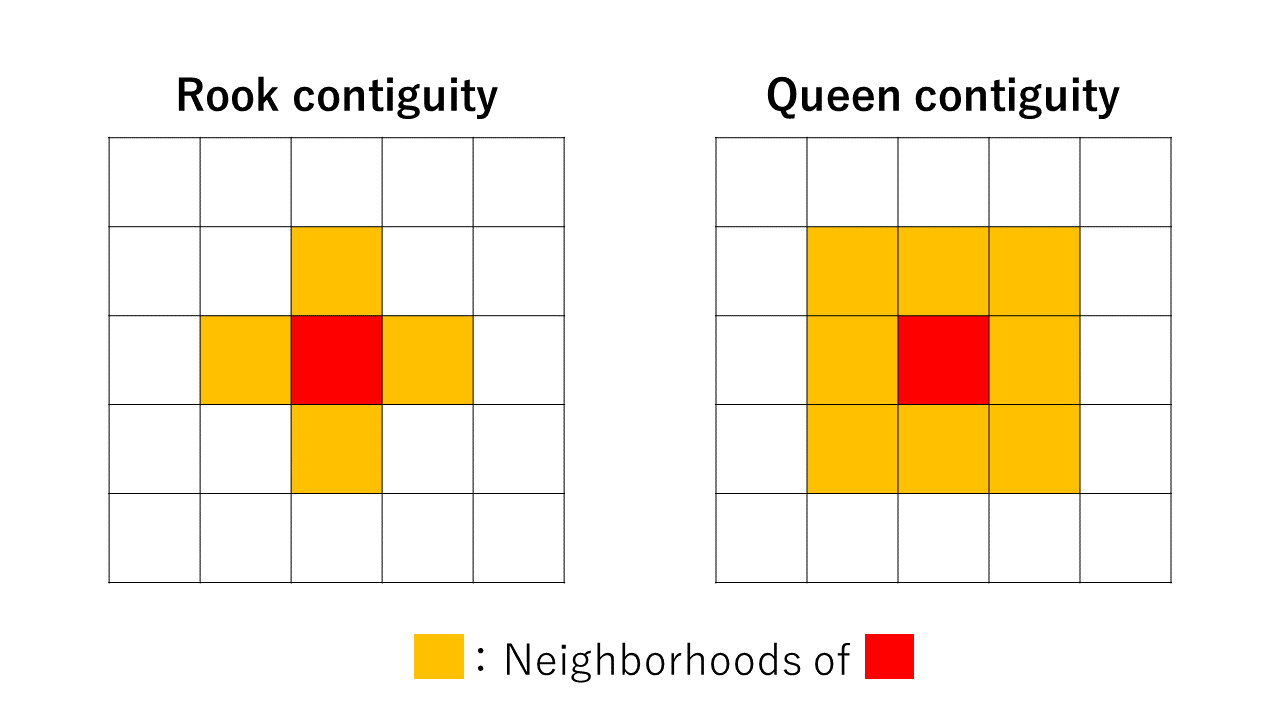
\includegraphics[width = 10cm]{adj.png}
		\caption{Rook contiguity and Queen contiguity\label{fig:contiguity}}
	\end{center}
\end{figure}

Now, consider a variable $X$, and suppose that we have sample data $\{X_1, \ldots, X_n\}$ of size $n$, where the subscript denotes each spatial unit.
Further, let $w_{ij}$ $(1 \le i,j \le n)$ be positive constants satisfying
\begin{align*}
\text{(i)} & \quad w_{ii} = 0  \;\; \text{for all $i$}\\
\text{(ii)} &\quad  w_{ij} \ge 0 \;\; \text{if $i$ and $j$ are close}\\
\text{(iii)} &\quad  w_{ij} = 0 \;\; \text{if $i$ and $j$ are distant enough}\\
\text{(iv)} &\quad  \sum_{j = 1}^n w_{ij} =1 \;\; \text{for all $i$}.
\end{align*} 
Such $w_{ij}$ is called the \textbf{spatial weight\index{spatial weight}} between $i$ and $j$.
Using the spatial weight, we can define the weighted ``neighborhood average'' of $X$ around unit $i$ by
\[
	X_i^* \equiv \sum_{j=1}^n w_{ij} X_j.
\]
Note that $i$ is not included in its own neighborhood ($w_{ii} = 0$).

\subsection*{Examples of spatial weights}
\paragraph{Polygon data}
In the case of polygon data, a commonly used spatial weight is as follows:
\[
	\begin{array}{ll}
	w_{ij} = \frac{1}{\text{\# of adjacent districts to $i$}}& \text{ if $j$ is adjacent to $i$} \\
	& \\
	w_{ij} = 0 &  \text{ if $j$ is not adjacent to $i$.} 
	\end{array}
\]
With this spatial weight, $X_i^*$ can be interpreted as the average of $X$ over the districts that are adjacent to $i$.
Note that the requirements $w_{ii} = 0$ and $\sum_{j = 1}^n w_{ij} =1$ for all $i$ means that there are no isolated districts, such as islands.
The latter condition is introduced for expositional simplicity, and can be relaxed in practice.

\paragraph{Point data}
In the case of point data, we first need to calculate the distance between every pair of spatial units, say $d(i,j)$.
Define,
\[
	\begin{array}{ll}
	v_{ij} = \frac{1}{d(i,j)^r}& \text{ if $d(i,j) \leq q $ and $j \neq i$} \\
	& \\
	v_{ij} = 0 &  \text{ otherwise } 
	\end{array}
\]
where $r$ is some positive number, which is typically 1 or 2, and $q$ is a pre-specified threshold value such that the objects with distance larger than $q$ are assumed to be independent.
Note that the $v_{ij}$'s defined above do not generally satisfy $\sum_{j = 1}^n v_{ij} = 1$.
Thus, we normalize them in the following way:
\[
	w_{ij} = \frac{v_{ij}}{\sum_{j' = 1}^n v_{ij'}}.
\]
This type of spatial weight is often called the distance-based spatial weight.
\bigskip

An $n \times n$ matrix $W_n$ whose $(i,j)$-th entry is given by $w_{ij}$ is called the \textbf{spatial weight matrix\index{spatial weight matrix}}: namely,
\[
	W_n = \left(\begin{array}{cccc}
		0            & w_{12} & \cdots & w_{1n} \\
		w_{21} &  0           & \cdots & w_{2n} \\
		\vdots    & \vdots    & \ddots & \vdots \\
		w_{n1} & w_{n2} & \cdots & 0
		\end{array}\right)
\]
One can view that the spatial weight matrix $W_n$ is a spatial version of the weighted social interaction matrix $G_n$.
Note that $W_n$ is not necessarily a symmetric matrix.
Using the spatial weight matrix, we can simply write $(X^*_1, \ldots, X_n^*)^\top = W_n \mbf{X}_n$, where  $\mbf{X}_n = (X_1, \ldots, X_n)^\top$.
\bigskip

Now, we are ready to more formally describe the definition of spatial autocorrelation.
We say that there exists a positive (resp. negative) spatial autocorrelation in the data if $\mbf{X}_n$ and $W_n \mbf{X}_n$ are positively (resp. negatively) correlated.
As one may notice, the determination of the existence of spatial autocorrelation is dependent and sensitive to the (somewhat arbitrarily) chosen spatial weights matrix $W_n$.

\subsection{Moran's I and Geary's C}

There are two major statistics to measure the magnitude of spatial autocorrelation.
The one is \textbf{Moran's I\index{Moran's I}} statistic, and the other is \textbf{Geary's C\index{Geary's C}} statistic, which are defined by
\[
	I \equiv \frac{\sum_{i=1}^n \sum_{j = 1}^n w_{ij}(X_i - \bar{X}_n) (X_j - \bar{X}_n)}{\sum_{i=1}^n (X_i - \bar{X}_n)^2}
\]
and
\[
	C \equiv \frac{n - 1}{2 n} \frac{\sum_{i=1}^n \sum_{j = 1}^n w_{ij}(X_i - X_j )^2}{\sum_{i=1}^n (X_i - \bar{X}_n)^2}
\]
respectively, where $\bar X_n = n^{-1}\sum_{i=1}^n X_i$.
Since Moran's I is a spatial extension of the standard (i.e., Pearson's) correlation coefficient between $\mbf{X}_n$ and $W_n \mbf{X}_n$, $I$ takes the value on the range $[-1, 1]$:
\[
\begin{array}{ll}
	\;\;\;0 < I \le 1 & \text{Positive spatial autocorrelation} \\
	\;\;\;\;\;\; I = 0 & \text{No spatial autocorrelation} \\
	-1 \leq I < 0 & \text{Negative spatial autocorrelation.}
\end{array}
\]
On the other hand, Geary's C ranges in value from $0$ to $2$, and the degree of spatial autocorrelation decreases as $C$ increases:
\[
\begin{array}{lc}
	1 < C \le 2 & \text{Negative spatial autocorrelation} \\
	\;\;\; C = 1 & \text{No spatial autocorrelation} \\
	0 \leq C < 1 & \text{Positive spatial autocorrelation.}
\end{array}
\]

Figure \ref{fig:IandC} provides numerical examples of Moran's I and Geary's C statistic based on the rook contiguity-based spatial weight.
\begin{figure}[h!]
	\begin{center}
		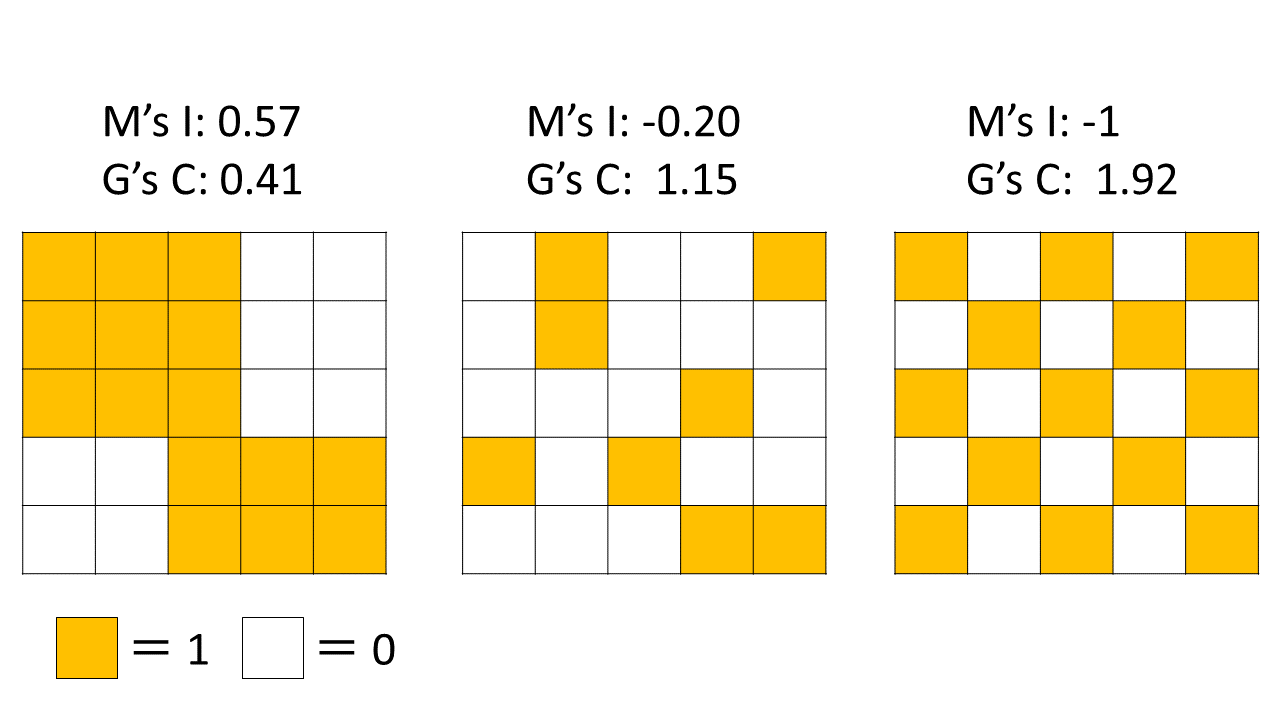
\includegraphics[width = 12cm]{IandC.png}
		\caption{Numerical examples: Moran's I and Geary's C\label{fig:IandC}}
	\end{center}
\end{figure}

\section{Spatial random variables}
\subsection{Spatial stochastic process}
In applications, it is mostly the case that $X$ is a random variable rather than a non-stochastic variable.
Suppose that each realized value of $X$ is uniquely characterized by its location $s$ in $\mathbb{R}^2$, and we may write $X \equiv X(s)$.
The collection of random variables $\{X(s) : s \in \mcl{S}_n\}$ is called as a \textbf{spatial stochastic process\index{spatial stochastic process}} (random field) with the sampling region $\mcl{S}_n \subseteq \mathbb{R}^2$.
The sampling region $\mcl{S}_n$ can be dependent on the sample size $n$, and it is usually required that $\mcl{S}_n$ expands as $n$ increases in each direction in $\mathbb{R}^2$, as stated below.

If $X(s)$ is independent of $X(s')$ for all $s \neq s'$, a random sample $\{X_1, \ldots, X_n\}$ of $X$ from $n$ distinct locations $\{s_i \in \mcl{S}_n: 1 \le i \le n\}$, where $X_i \equiv X(s_i)$, can be virtually treated as the standard non-spatial data.
In this case, letting $\sigma^2(s) = \Var(X(s)) < \infty$, we have
\[
	\Var\left( \bar X_n\right) = \frac{1}{n} \bar{\sigma}^2_n \to 0,
\]
as $n \to \infty$, where $\bar{\sigma}^2_n = \frac{1}{n}\sum_{i=1}^n \sigma^2(s_i)$.
Thus, by Chebyshev's inequality (\ref{eq:chevyshev}), for any positive constant $\kappa >0$,
\[
	\Pr\left( \left| \bar X_n - \E \bar X_n \right| \ge \kappa \right) \le \frac{\Var(\bar X_n)}{\kappa^2} \to 0,
\]
implying that the WLLN holds: $\bar X_n \overset{p}{\to} \E \bar X_n$. 
Similarly, it can be straightforwardly verified that the CLT also holds (under some additional regularity conditions).

However, the above argument is not realistic for spatial data in that $\{X_1, \ldots, X_n\}$ are independent.
It is clear that if the dependence between the variables is strong such that $\Var\left( \bar X_n\right)$ does not converge to zero, standard large sample theory would not be applicable.
In contrast, even when they are dependent, it is possible to show that the law of large numbers and the central limit theorem hold only if the degree of dependence is sufficiently weak.

Here, for simplicity, assume that the data points are located on a regular lattice in $\mathbb{R}^2$, and that $\Cov(X(s), X(s')) \equiv C(s, s') = \rho$, where $0 < \rho < \infty$, if $(s, s')$ are neighboring grid-points, and $C(s, s') = 0$ otherwise.

\begin{figure}[h!]
	\begin{center}
		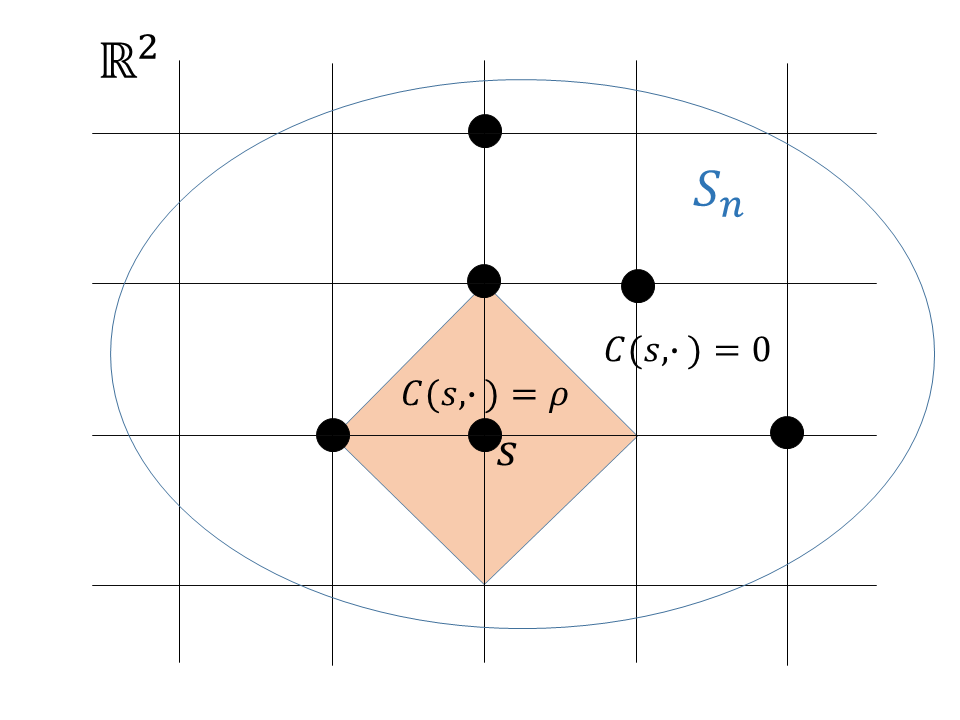
\includegraphics[width = 9cm]{sprnd.png}
		\caption{A type of weak spatial dependence}
	\end{center}
\end{figure}

The assumption that the covariance between the variables at two different locations depends only on the distance between them is called \textbf{isotropy\index{isotropy}} (i.e., directions do not matter).

Then, noting that there are at most four neighboring data points for each $s$, we have
\begin{align*}
	\Var(\bar X_n) 
	& = \frac{1}{n^2}\sum_{i=1}^n \sigma^2(s_i) + \frac{1}{n^2}\sum_{i = 1}^n \underbrace{\sum_{j \neq i}^n C(s_i, s_j)}_{\le \: 4\rho} \\
	& \le \frac{1}{n}\bar{\sigma}_n^2 + \frac{1}{n} 4 \rho \to 0
\end{align*}
as $n \to \infty$.
Therefore, the WLLN holds, and so does CLT with some weak additional conditions.
Although the spatial dependence structure introduced in this example is too simplistic for real data, more realistic dependence structures are proposed in the literature, for example, \textit{spatial mixing} and \textit{spatial near epoch dependence}, which are both natural spatial extensions of the dependence concept used in time series analysis.

\subsection{Spatial sampling}
 
 As mentioned above, if the degree of spatial dependence is sufficiently weak, one can rely on standard large sample theory.
It is important to note that such assumption implicitly requires that the sampling region must be (weakly) expanding: $\mcl{S}_n \subseteq \mcl{S}_{n + 1} \subseteq \cdots \subseteq \mbb{R}^2$, with the minimum distance between observations being fixed away from zero.
Large sample theory based on this type of data sampling framework is called \textbf{increasing domain asymptotics\index{increasing domain asymptotics}}.

On the other hand, suppose that the sampling region is fixed and bounded:  $\mcl{S}_n = \mcl{S}_{n + 1}  = \cdots \subset \mbb{R}^2$.
In this case, as the sample size $n$ increases, the observations get denser and denser.
Consequently, for a given data point $s$, the number of observations that are spatially dependent of $s$ can increase to infinity as $n$ increases.
This case is called \textbf{infill asymptotics\index{infill asymptotics}} (or fixed domain asymptotics).
As can be easily imagined, asymptotic theory under the infill asymptotics is much more involved than the one under the increasing domain asymptotics.
The infill asymptotic theory has been an important research field particularly in the literature on high frequency time series.

\begin{figure}[h!]
	\begin{center}
		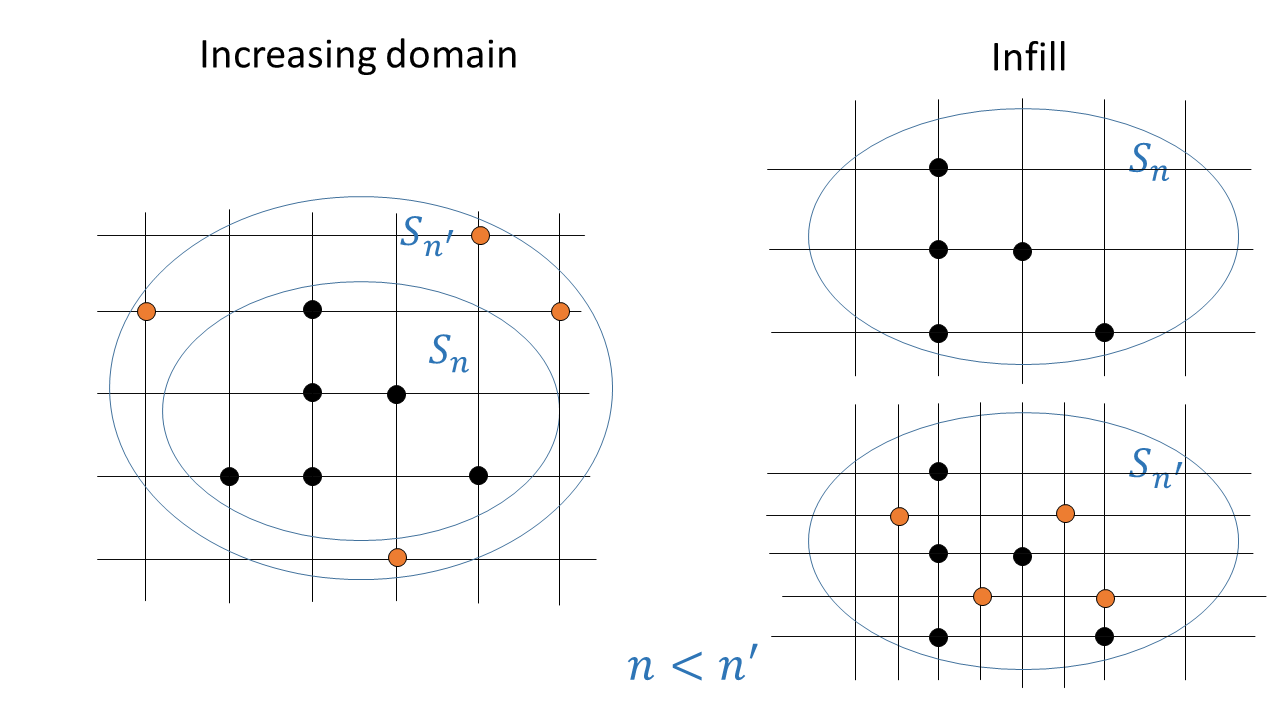
\includegraphics[width = 12cm]{asymptotics.png}
		\caption{Increasing domain asymptotics and infill asymptotics}
	\end{center}
\end{figure}
%%%%%%%%%%%%%%%%%%%%%%%%%%%%%%%%%%%%%%%%%%%%%%%%%

\chapter{Spatial Econometrics}\label{chap:spatial_econometrics}

Spatial econometrics is a subfield of econometrics that deals with spatial interaction (spatial autocorrelation) across spatial units.
Spatial econometric tools have become popular as empirical data analysis techniques for a range of diverse topics, including local economic growth, property markets, local competition between municipalities, local crime, and so forth. 
There are two most commonly used spatial econometric models: the \textbf{spatial lag model\index{spatial lag model}} (or spatial autoregressive model) and the \textbf{spatial error model\index{spatial error model}}.
In terms of the three types of social interaction effects classified by \cite{manski1993identification}, the spatial lag model is a model that accounts for possible endogeneity of spatial interaction, and the spatial error model accounts for the spatially correlated effects.

\section{Spatial lag model}\label{sec:SLM}

Let $Y$ be a dependent variable of interest, and $X$ be the vector of explanatory variables including a constant term.
Suppose that a sample $\{(Y_i,X_i): 1 \le i \le n\}$ of size $n$ is observed.
Further, let $w_{ij}$ be a spatial weight term between $i$ and $j$.
Recall that $w_{ii} = 0$ for normalization.
Then, the following model is called the \textbf{spatial lag model\index{spatial lag model}} (SLM):
\begin{align}\label{eq:slm}
	Y_i = \rho_0 \sum_{j = 1}^n w_{ij} Y_j + X_i^\tr\beta_0 + \eps_i, \;\; i = 1,\ldots,n.
\end{align}
Here, $\rho_0$ is a parameter that captures the spatial endogenous effect, $\beta_0$ is a vector of unknown coefficients, and $\eps$ is an unobserved random variable such that $\E \eps = 0$.
The SLM assumes that the average outcome of the neighboring districts influences on own outcome.

For example, imagine that there are two districts, which are almost identical in terms of sociodemographic and economic characteristics.
Suppose that one of them is surrounded by areas with higher crime rates, and the other is  located in a low crime rate area.
Then, if the crime rate of the former district is higher than that of the latter, this suggests the existence of spatial endogenous effect, and the spatial parameter $\rho_0$ will be estimated as positive.

Let $W_n = (w_{ij})_{i,j = 1}^n$ be the spatial weight matrix, and write $\mbf{Y}_n = (Y_1, \ldots, Y_n)^\top$�C$\mbf{X}_n = (X_1, \ldots , X_n)^\top$�Cand $\mcl{E}_n = (\eps_1, ...., \eps_n)^\top$.
Then, we can rewrite model \eqref{eq:slm} in matrix form as
\[
	\mbf{Y}_n =  \rho_0 W_n \mbf{Y}_n + \mbf{X}_n \beta_0 + \mcl{E}_n.
\]
As one can see, the form of the SLM is quite similar to that of the social interaction model in \eqref{eq:bramat}.
Indeed, the SLM can be interpreted in the same manner as in the social interaction model.
That is, the SLM can be viewed as a game model of complete information with the realized outcomes $\{Y_1, \ldots, Y_n \}$ being a result of Nash equilibrium behavior.\footnote{
	In this case, the source of spatial autocorrelation is the presence of local strategic interaction.
	However, in many applications, what mechanisms generate the spatial autocorrelation is less concerned, and researchers often introduce a model like \eqref{eq:slm} a priori.
}
In addition, if $|\rho_0| < 1$ and the spatial weight matrix is normalized such that each row sums to unity, the matrix $I_n - \rho_0 W_n$ is nonsingular, and thus the inverse matrix 
$(I_n - \rho_0 W_n)^{-1}$ exists.
Thus, the reduced-form of the SLM can be obtained by
\[
	\mbf{Y}_n =  (I_n - \rho_0 W_n)^{-1}\mbf{X}_n \beta_0 + (I_n - \rho_0 W_n)^{-1}\mcl{E}_n.
\]

By Neumann series expansion (Appendix \ref{sec:neumann}), we have 
\[
	(I_n - \rho_0 W_n)^{-1}\mbf{X}_n\beta_0 = \mbf{X}_n\beta_0 + \rho_0 W_n \mbf{X}_n\beta_0 + \rho_0^2 W_n^2\mbf{X}_n\beta_0 + \cdots.
\]
Similarly to the social interaction model, the second term on the right-hand side represents the effect of the neighbors' characteristics, and the third term is the effect from the neighbors' neighbors' characteristics, and so forth.
This implies that a marginal increase in $X$ affects not only own outcome $Y$ but the outcomes of the others, and vice versa.
In the context of spatial econometrics, the matrix $(I_n - \rho_0 W_n)^{-1} $ is called the \textbf{spatial multiplier} matrix.

\subsection{Maximum likelihood estimation}

 For the same reason mentioned in Section \ref{sec:estimation_soc}, a simple OLS estimator that regresses $\mbf{Y}_n$ on $(W_n \mbf{Y}_n, \mbf{X}_n)$ is not consistent because of the endogeneity of $W_n \mbf{Y}_n$.
 To deal with this problem, one may use a maximum likelihood approach.
 Specifically, assume that the error terms $(\eps_1, \ldots , \eps_n)$ are IID as normal $N(0, \sigma_0^2)$.
 Then, the conditional joint distribution of $\mbf{Y}_n$ given $\mbf{X}_n$ is characterized by
 \[
 	\mbf{Y}_n \mid \mbf{X}_n \sim \mbf{N}\left( (I_n - \rho_0 W_n)^{-1}\mbf{X}_n \beta_0, \; (I_n - \rho_0 W_n)^{-1}(I_n - \rho_0 W_n^\top)^{-1}\sigma_0^2\right),
 \]
and one can show that the log-likelihood function of the SLM is given by
\begin{align*}
 	\ell^{SLM}_n(\rho, \beta, \sigma^2) 
 	&= -\frac{n}{2} \log (2\pi) -\frac{n}{2} \log\sigma^2 + \log | I_n - \rho W_n| \\
 	& \quad - \frac{1}{2\sigma^2} ((I_n - \rho W_n)\mbf{Y}_n - \mbf{X}_n \beta)^\top ((I_n - \rho W_n)\mbf{Y}_n - \mbf{X}_n \beta),
 \end{align*}
where $|A_n|$ denotes the determinant of the matrix $A_n$.
Then, we can obtain a consistent estimator of $(\rho_0, \beta_0, \sigma_0^2)$ as the maximizer of the above log-likelihood function; see \cite{lee2004asymptotic} for details on the theoretical properties of this estimator.

However, this maximum likelihood estimation has two serious drawbacks.
First, the assumption that $(\eps_1, \ldots , \eps_n)$ are IID normal is very restrictive for spatial data, since spatial units are naturally correlated and heterogeneous in several characteristics, such as area size and population.
Second, the computation of the objective function $\ell^{SLM}_n(\rho, \beta, \sigma^2)$ can be quite expensive when the sample size is not small; calculating the determinant of a large matrix is very time-consuming and often computationally intractable.
Fortunately, as described below, one can obtain a consistent estimator of the model parameters by the 2SLS method of \cite{kelejian1998generalized}, without relying on the IID normality assumption.

\subsection{2SLS estimation}\label{subsec:2sls}

To simplify the exposition, in the following we assume that the regressor $X$ is non-stochastic and bounded in absolute value.\footnote{
	The assumption of non-stochastic regressors is often adopted in the literature of spatial econometrics, partly for the purpose of avoiding tedious technical discussions on the underlying spatial random process.
	In the non-stochastic regressors framework, we should interpret the analysis as being conditional on the realization of these variables.
}
Then, since $\E \eps  = 0$, this automatically implies that the regressor $X$ is exogenous: $\E[X\eps] = X \E[\eps] = 0$.

Suppose that the matrix $I_n - \rho_0 W_n$ is nonsingular with $|\rho_0| < 1$.
Then, we have
\begin{align*}
	W_n \mbf{Y}_n 
	& = W_n(I_n - \rho_0 W_n)^{-1}\mbf{X}_n\beta_0 + W_n (I_n - \rho_0 W_n)^{-1}\mcl{E}_n\\
	& = W_n\mbf{X}_n\beta_0 + \rho_0 W^2_n\mbf{X}_n\beta_0 + \rho^2_0 W^3_n\mbf{X}_n\beta_0 + \cdots +  W_n (I_n - \rho_0 W_n)^{-1}\mcl{E}_n.
\end{align*}
The first line implies that the ideal instrumental variable for the endogenous regressor $W_n\mbf{Y}_n$ is $W_n(I_n - \rho W_n)^{-1}\mbf{X}_n\beta$.
However, we cannot use this since $\rho_0$ and $\beta_0$ are unknown in practice.
The second line shows that the ideal instrument $W_n(I_n - \rho_0 W_n)^{-1}\mbf{X}_n\beta_0$ is expressed as a linear combination of $\{W_n\mbf{X}_n, W^2_n\mbf{X}_n, \ldots\}$.
Thus, a subset of columns of $\{W_n\mbf{X}_n, W^2_n\mbf{X}_n, \ldots\}$ can be used as a feasible and reasonable instrument for $W_n\mbf{Y}_n$.
Specifically, let $\mbf{Z}_{n1}$ be a matrix of instrumental variables composed of a subset of linearly independent columns of $\{W_n\mbf{X}_n, W^2_n\mbf{X}_n, \ldots\}$, and define $\mbf{Z}_n = (\mbf{X}_n, \mbf{Z}_{n1})$.
Then, a consistent estimator of $\theta_0 = (\rho_0, \beta_0^\top)^\top$ can be obtained the 2SLS method as follows.
In the first step, we regress the endogenous variable $W_n \mbf{Y}_n$ on $\mbf{Z}_n$, and obtain the predicted value of $W_n\mbf{Y}_n$ by 
\[
	\hat{W_n\mbf{Y}_n} = \mbf{Z}_n(\mbf{Z}_n^\top \mbf{Z}_n)^{-1}\mbf{Z}_n^\top W_n \mbf{Y}_n.
\]
In the second step, $\theta$ is estimated by a linear regression of $\mbf{Y}_n$ on $(\hat{W_n\mbf{Y}_n}, \mbf{X}_n)$.
Let $\hat \theta_n$ be the resulting estimator of $\theta_0$.
In the same manner as in \eqref{eq:2slssoc}, we can derive the closed-form expression for the 2SLS estimator $\hat \theta_n$ as
\begin{align}\label{eq:2sls}
	\hat \theta_n = \left[\mbf{H}_n^\top \mbf{Z}_n(\mbf{Z}_n^\top \mbf{Z}_n)^{-1}\mbf{Z}_n^\top \mbf{H}_n  \right]^{-1}\mbf{H}_n^\top \mbf{Z}_n(\mbf{Z}_n^\top \mbf{Z}_n)^{-1}\mbf{Z}_n^\top\mbf{Y}_n,
\end{align}
 where $\mbf{H}_n = (W_n\mbf{Y}_n, \mbf{X}_n)$. 
Asymptotic properties of the 2SLS estimator \eqref{eq:2sls} can be derived in the same way as in Section \ref{sec:2slsAsymptotics}.

\section{Spatial error model}\label{sec:SEM}

It is highly possible that the unobserved determinant of $Y$, $\eps$, involves some spatial factors.
If they are spatially correlated, the model has spatial correlated effects.
To account for the spatial correlated effects (i.e., spatial autocorrelation of $\eps$), we can consider the following model:
\begin{align}\label{eq:sem}
\begin{split}
	Y_i  & = X_i^\tr\beta_0 + \eps_i \\
	\eps_i & = \lambda_0 \sum_{j = 1}^n w_{ij} \eps_j + u_i, \;\; i = 1,\ldots,n
\end{split}
\end{align}
where $u_i$ is an idiosyncratic (non-spatial) error term such that $\E u = 0$, and $\lambda_0$ is the parameter that captures the spatial correlated effect.
The above model is called the \textbf{spatial error model\index{spatial error model}} (SEM).
In contrast to the SLM, the SEM does not admit the existence of spatial multiplier effects; that is, in SEM, an increase in own $X$ solely influences on own $Y$ and not on the others' outcomes.
Thus, these two models have quite different policy implications.

\subsection{Maximum likelihood estimation}
Again, we retain the assumption that $X$ is non-stochastic.
When the matrix $I_n - \lambda_0 W_n$  is nonsingular with $|\lambda_0| < 1$, the SEM can be re-written in matrix form as
\[
	\mbf{Y}_n =  \mbf{X}_n \beta_0 + (I_n - \lambda_0 W_n)^{-1}U_n,
\]
where $U_n = (u_1, \ldots, u_n)^\top$.
Then, since each $\eps$ can be expressed as a linear combination of $(u_1, \ldots, u_n)$, we have $\E \eps = 0$, and thus $\E[X \eps] = 0$ holds; that is, $X$ is exogenous.
Therefore, for the estimation of SEM, a simple OLS regression yields a consistent estimate of $\beta_0$, although not efficient and uninformative for the spatial parameter $\lambda_0$.

In order to estimate $\lambda_0$, we can consider a maximum likelihood estimation.
Assuming now that $(u_1, \ldots , u_n)$ are IID as normal $N(0, \sigma_0^2)$, the conditional joint distribution of $\mbf{Y}_n$  given $\mbf{X}_n$ is characterized by
\[
	\mbf{Y}_n \mid \mbf{X}_n \sim \mbf{N}\left(\mbf{X}_n \beta_0, \; (I_n - \lambda_0 W_n)^{-1}(I_n - \lambda_0 W_n^\top)^{-1}\sigma^2_0 \right).
\]
After some calculations, the log-likelihood function of the SEM can be obtained as follows:
\begin{align*}
	\ell^{SE}_n(\lambda, \beta, \sigma^2) 
	& = -\frac{n}{2} \log (2\pi) -\frac{n}{2} \log\sigma^2 + \log | I_n - \lambda W_n| \\
	& \quad - \frac{1}{2\sigma^2} (\mbf{Y}_n - \mbf{X}_n \beta)^\tr(I_n - \lambda W_n)^\tr (I_n - \lambda W_n) (\mbf{Y}_n  - \mbf{X}_n \beta).
\end{align*}
By maximizing the above log-likelihood function, we can obtain a consistent estimator of $(\lambda_0, \beta_0, \sigma^2_0)$.
However, the IID normality assumption is restrictive as mentioned above.
Also, again since the log-likelihood function involves the determinant of the matrix $I_n - \lambda W_n$, there can be significant difficulties in the practical computation of this estimator.
In order to overcome this issue, \cite{kelejian1999generalized} developed a method of moments (MM) estimator that is not dependent on the IID normality assumption and is computationally easy irrespective of the size of the sample.

\subsection{Method of moments estimation}\label{subsec:mm}

The estimation procedure of the MM estimator is implemented in two steps.
The first step estimates the coefficients $\beta_0$ by the OLS regression of $\mbf{Y}_n$ on $\mbf{X}_n$, and let $\hat \beta_n$ be the resulting estimator.
Here, we assume that $(u_1, \ldots , u_n)$ are homoskedastic with variance $\E[u_i^2] = \sigma_0^2$ for all $i$.\footnote{
	The homoskedasticity assumption is introduced for simplicity.
	A heteroskedasticity-robust version of the estimation procedure is explained in \cite{kelejian2010specification}.
}
In the second step, we estimate $(\lambda_0, \sigma_0^2)$ by the MM approach.
The estimator is based on the following three moment equalities: 
\begin{align*}
	\E\left[ U_n^\top U_n /n \right] = \sigma_0^2, \;\; \E\left[ \bar U_n^\top \bar U_n /n \right] =  \sigma_0^2  \mrm{trace}\left\{ W_n^\top W_n/n \right\}, \;\;  \E\left[ \bar U_n^\top U_n/n \right] = 0,
\end{align*}
where $\bar U_n = W_n U_n$.
Note that for any $n \times 1$ vectors $A_n$ and $B_n$, $A_n^\top B_n = \mrm{trace}\{ A_n B_n^\top \}$.
In the third equality, we have used the fact that the diagonal elements of $W_n$ are zero.
Let $\bar{\mcl{E}}_n = W_n \mcl{E}_n$ and $\bar{\bar{\mcl{E}}}_n = W_n W_n \mcl{E}_n$.
Since we have
\[
	U_n = \mcl{E}_n - \lambda_0 \bar{\mcl{E}}_n\; \text{ and }\; \bar U_n = \bar{\mcl{E}}_n - \lambda_0 \bar{\bar{\mcl{E}}}_n,
\]
 the above three equalities can be rewritten in terms of $\mcl{E}_n$ as
\begin{align*}\renewcommand{\arraystretch}{1.8}
\begin{array}{lllll}
	\E\left[ \mcl{E}_n^\top \mcl{E}_n /n\right] 
	& - 2\lambda_0 \E\left[ \mcl{E}_n^\top \bar{\mcl{E}}_n/n \right] 
	& +  \lambda^2_0 \E\left[ \bar{\mcl{E}}_n^\top \bar{\mcl{E}}_n/n \right] 
	& - \sigma^2_0 
	& = 0,\\
	\E\left[ \bar{\mcl{E}}_n^\top \bar{\mcl{E}}_n/n \right] 
	& - 2\lambda_0 \E\left[ \bar{\mcl{E}}_n^\top \bar{\bar{\mcl{E}}}_n/n \right] 
	& +  \lambda^2_0 \E\left[ \bar{\bar{\mcl{E}}}_n^\top \bar{\bar{\mcl{E}}}_n/n \right] 
	& - \sigma^2_0 \mrm{trace}\left\{ W_n^\top W_n/n \right\} 
	& = 0, \\
	\E\left[ \bar{\mcl{E}}_n^\top \mcl{E}_n/n \right] 
	& - \lambda_0 \E\left[ \bar{\mcl{E}}_n^\top \bar{\mcl{E}}_n/n + \bar{\bar{\mcl{E}}}_n^\top \mcl{E}_n/n\right] 
	& +  \lambda^2_0 \E\left[ \bar{\mcl{E}}_n^\top \bar{\bar{\mcl{E}}}_n/n \right]  
	&
	& = 0.
\end{array}
\end{align*}
Equivalently,
\begin{align*}
	\Gamma_n (\lambda_0, \lambda_0^2, \sigma_0^2)^\top - \gamma_n = \mbf{0},
\end{align*}
where
\[\renewcommand{\arraystretch}{1.8}
	\Gamma_n \equiv \left(
	\begin{array}{ccc}
	2 \E\left[ \mcl{E}_n^\top \bar{\mcl{E}}_n/n \right] 
	& - \E\left[ \bar{\mcl{E}}_n^\top \bar{\mcl{E}}_n/n \right] 
	& 1 \\
	2 \E\left[ \bar{\mcl{E}}_n^\top \bar{\bar{\mcl{E}}}_n/n \right] 
	& - \E\left[ \bar{\bar{\mcl{E}}}_n^\top \bar{\bar{\mcl{E}}}_n/n \right] 
	& \mrm{trace}\left\{ W_n^\top W_n/n \right\}  \\
	\E\left[ \bar{\mcl{E}}_n^\top \bar{\mcl{E}}_n/n + \bar{\bar{\mcl{E}}}_n^\top \mcl{E}_n/n\right] 
	& - \E\left[ \bar{\mcl{E}}_n^\top \bar{\bar{\mcl{E}}}_n/n \right]  
	& 0
	\end{array}
	\right)
	\qquad
	\gamma_n \equiv \left(\begin{array}{c}
	\E\left[ \mcl{E}_n^\top \mcl{E}_n /n\right] \\
	\E\left[ \bar{\mcl{E}}_n^\top \bar{\mcl{E}}_n/n \right] \\
	\E\left[ \bar{\mcl{E}}_n^\top \mcl{E}_n/n \right]
	\end{array}
	\right).
\]\renewcommand{\arraystretch}{1}
Thus, the true value of $(\lambda, \sigma^2)$ can be characterized as the minimizer of the objective function $|| \Gamma_n (\lambda, \lambda^2, \sigma^2)^\top - \gamma_n ||^2$, where $|| \cdot ||$ denotes the Euclidean norm.
This implies that we can estimate $(\lambda_0, \sigma^2_0)$ by minimizing the sample analog of $|| \Gamma_n (\lambda, \lambda^2, \sigma^2)^\top - \gamma_n ||^2$, where the expectations in the definition of $\Gamma_n$ and $\gamma_n$ are dropped, and $\mcl{E}_n$ is replaced by $\hat{\mcl{E}}_n = \mbf{Y}_n - \mbf{X}_n\hat \beta_n$.
Let the resulting MM estimator of  $(\lambda_0, \sigma^2_0)$ be $(\hat \lambda_n, \hat \sigma_n^2)$.
\cite{kelejian1999generalized} proved that the MM estimator $(\hat \lambda_n, \hat \sigma_n^2)$ is consistent under mild regularity conditions.
The limiting distribution of $(\hat \lambda_n, \hat \sigma_n^2)$ is complicated and is omitted here (see, e.g., \cite{kelejian2010specification}).
\bigskip

Once a consistent estimate $(\hat \lambda_n, \hat \sigma_n^2)$ is obtained, we can use a generalized least squares (GLS) estimator of $\beta_0$ to obtain a more efficient estimate.
Specifically, let
\[
	\hat \Omega_n \equiv (I_n - \hat \lambda_n W_n)^{-1}(I_n - \hat \lambda_n W_n^\top)^{-1} .
\]
Then, the GLS estimator of $\beta_0$ is defined by
\begin{align}\label{eq:gls}
	\hat \beta_n^{GLS} = \left[\mbf{X}_n^\top \hat \Omega_n^{-1} \mbf{X}_n \right]^{-1} \mbf{X}_n^\top \hat \Omega_n^{-1} \mbf{Y}_n.
\end{align}
The GLS estimator $\hat \beta_n^{GLS}$ is asymptotically efficient, with its covariance matrix being $ (\sigma^2/n)\left[\mbf{X}_n^\top \Omega_n^{-1} \mbf{X}_n / n \right]^{-1}$, where $\Omega_n \equiv (I_n - \lambda_0 W_n)^{-1}(I_n - \lambda_0 W_n^\top)^{-1}$.

\section{Empirical analysis with \textbf{R}: Household burglary in Tokyo}\label{sec:emp_burglar}

It is commonly observed that different locations sharing the same social and economic conditions do not necessarily experience the same crime intensity.
Instead, spatial clusters of crimes (i.e., ``hot spots'') exist.
Accordingly, it is important to incorporate spatial information in quantitative criminology research.
In this empirical analysis, we investigate the determinants of household burglary risk in Tokyo.

The dataset used here is the same as the one in \cite{hoshino2018semiparametric}.\footnote{
	The data files are available on request.
}
The variables used in the analysis are created from several data sources.
For crime data, we use the number of household burglaries recorded in 2011 by the Tokyo Metropolitan Police Department for each district in Tokyo.
The socio-demographic and economic information for each district are taken from the Census 2010 and the Commercial Statistics Survey 2009.
The definitions of the variables are summarized in the following table.
All variables are constructed at the district level.

\begin{center}
	\begin{tabular}{l|l|l}
		\multicolumn{3}{c}{ Variables and their definitions} \\ \hline\hline
				&  \multicolumn{1}{|c|}{\small Variable} &  \multicolumn{1}{|c}{\small Definition} \\ \hline
		\small Dependent variable & \small \textit{burglary} & ${\small 1,000\times }\dfrac{\text{{\small \# of recorded household burglaries}}}{\text{{\small \# of households}}}$ \\ 
		&  &  \\ 
		\small Explanatory variables & \small \textit{nhmem}  & \small Average number of household members. \\
													  & \small \textit{dnsty} & \small Residential density (\# of residences / Area of district). \\ 
		                                              & \small \textit{owner} & \small Portion of owner-occupied houses. \\
		                                              & \small \textit{elder}    & \small Portion of households headed by the elderly (over 65 years old). \\
		                                              & \small \textit{high}    & \small Portion of high-rise residential buildings. \\ 
		                                              & \small \textit{manag} & \small \# of workers in managerial positions / Labor force population. \\ 
		                                              & \small \textit{retail}      & \small Total area of retail stores in district / Area of district. \\ 
												     & \small Ward dummies & \small Dummies for the 23 special wards of Tokyo.$^\dagger$ \\ \hline
	\end{tabular}
	\begin{flushleft}
	($\dagger$: {\small Here, 22 dummy variables are introduced. Nerima ward is omitted as a benchmark.)}
	\end{flushleft}
\end{center}

After deleting the observations with missing values, a sample of $n = 3025$ observations is used in this analysis.
With this dataset, we estimate SLM \eqref{eq:slm} and SEM \eqref{eq:sem} by the 2SLS method and the MM method, respectively.
The spatial weight matrix is constructed based on Queen-contiguity and is row-normalized.

Set the \textbf{R} working directory appropriately, and read the csv files.
\begin{lstlisting}[basicstyle=\ttfamily\footnotesize, frame=single]
# Data #

 data <- as.data.frame(read.csv("TokyoCrime.csv"))
 n    <- nrow(data) # sample size (n = 3025)

# Spatial weight matrix #

 W <- as.matrix(read.csv("TokyoCrime_W.csv", header = FALSE))
\end{lstlisting}
The variables used are defined as follows.
\begin{lstlisting}[basicstyle=\ttfamily\footnotesize, frame=single]
# Variables #

 Y  <- data$burglary
 X1 <- with(data, cbind(nhmem, dnsty, owner, elder, high, manag, retail))

 ward23 <- as.numeric(data$ward)
 wdum   <- matrix(0, n, 22)
 for(i in 1:22) wdum[,i] <- ifelse(ward23 == i, 1, 0)

 X <- cbind(1, X1, wdum)
\end{lstlisting}

We first estimate the SLM.
In accordance with the notation in Section \ref{subsec:2sls}, define the variables as follows.
\begin{lstlisting}[basicstyle=\ttfamily\footnotesize, frame=single]
 H  <- cbind(W%*%Y, X)
 Z1 <- cbind(W%*%X1, W%*%W%*%X1, W%*%W%*%W%*%X1)
 Z  <- cbind(X, Z1)
\end{lstlisting}
As the instruments for $W_n \mbf{Y}_n$, we employ the first, second, and third-order spatial lags of the explanatory variables (excluding the constant and the ward dummies).
Then, following \eqref{eq:2sls}, we obtain the 2SLS estimate in the following manner.
\begin{lstlisting}[basicstyle=\ttfamily\footnotesize, frame=single]
# 2SLS estimation #

 P     <- Z%*%solve(t(Z)%*%Z)%*%t(Z)
 theta <- solve(t(H)%*%P%*%H)%*%t(H)%*%P%*%Y
\end{lstlisting}
We compute the covariance matrix of the 2SLS estimator under homoskedasticity.
Once the covariance matrix is obtained, we can then calculate the standard error and t-value of the estimated parameter.
\begin{lstlisting}[basicstyle=\ttfamily\footnotesize, frame=single]
# Covariance matrix under homoskedasticity #

 sigma2 <- mean((Y - H%*%theta)^2) 
 Q_ZZ   <- t(Z)%*%Z/n
 Q_ZH   <- t(Z)%*%H/n 
 Cov    <- (sigma2/n)*solve(t(Q_ZH)%*%solve(Q_ZZ)%*%Q_ZH)

 sd   <- diag(Cov)^0.5 # Standard error
 tval <- theta/sd      # t-value
\end{lstlisting}
The summary of the results is as follows. 
\begin{lstlisting}[basicstyle=\ttfamily\footnotesize, frame=single]
>  cbind(theta, sd, tval)
                     sd
        0.4257077087 0.18952982  2.246125184
        0.6074076919 0.23175842  2.620865663
nhmem  -0.1652634554 0.09324095 -1.772434221
dnsty   5.9766729090 3.18795297  1.874768216
owner   0.0733078500 0.16210661  0.452220004
elder   0.0625461529 0.35319744  0.177085524
high   -0.5562633330 0.12004293 -4.633870187
manag  -0.3134209803 0.92201410 -0.339930790
retail -0.4174281178 0.41219978 -1.012683981

== The results for the ward dummies are omitted to save space. ==
\end{lstlisting}
The results show that the spatial autocorrelation in the household burglary rate is positive and significant.
It indicates that a one-point increase in the average burglary rate of neighboring districts increases own district's burglary rate by about 0.4.
Among the other explanatory variables, we find that the \textit{high} variable significantly negatively affect the burglary rate.
This result would be a reflection of the fact that high-rise buildings are likely equipped with high-security system.
\bigskip

Next, we estimate the SEM.
The fist step of the estimation procedure is to estimate $\beta_0$ by OLS. 
\begin{lstlisting}[basicstyle=\ttfamily\footnotesize, frame=single]
# OLS estimation #

 beta <- lm(Y ~ X - 1)$coef
\end{lstlisting}
The second step is to implement the MM estimation.
In line with Section \ref{subsec:mm}, we define the following quantities.
\begin{lstlisting}[basicstyle=\ttfamily\footnotesize, frame=single]
 E  <- Y - X%*%beta
 E1 <- W%*%E
 E2 <- W%*%W%*%E

 Gam1 <- c(2*t(E)%*%E1/n,              -t(E1)%*%E1/n, 1)
 Gam2 <- c(2*t(E1)%*%E2/n,             -t(E2)%*%E2/n, sum(diag(t(W)%*%W))/n) 
 Gam3 <- c(t(E1)%*%E1/n + t(E2)%*%E/n, -t(E1)%*%E2/n, 0)
 Gam  <- rbind(Gam1, Gam2, Gam3)
 gam  <- c(t(E)%*%E/n, t(E1)%*%E1/n, t(E1)%*%E/n)
\end{lstlisting}
Then, the objective function to be minimized is defined as follows.
\begin{lstlisting}[basicstyle=\ttfamily\footnotesize, frame=single]
# Objective function in the MM estimation #

 ObjF <- function(param){

	g <- Gam%*%c(param[1], param[1]^2, param[2]^2) - gam
	sum(g^2)

	}
\end{lstlisting}
Here, the vector \texttt{param} is a 2-dimensional vector with its first element corresponding to the spatial parameter $\lambda$ and the second element to the standard error $\sigma$.
The minimizer of \texttt{ObjF} can be found by using the command \texttt{optim}.
To do this, we need to specify initial candidate values for $\lambda$ and $\sigma$, which are set to 0.5 and the standard deviation of the residuals (\texttt{sd(E)}), respectively.
\begin{lstlisting}[basicstyle=\ttfamily\footnotesize, frame=single]
 NLS    <- optim(c(0.5, sd(E)), ObjF)
 lambda <- NLS$par[1]
 sigma2 <- NLS$par[2]^2

>  c(lambda, sigma2)
[1] 0.1597388 0.9959481
\end{lstlisting}

Using these estimated values, we re-estimate $\beta_0$ by the GLS method.
Following \eqref{eq:gls}, the GLS estimate $\hat \beta_n^{GLS}$ is computed as follows.
\begin{lstlisting}[basicstyle=\ttfamily\footnotesize, frame=single]
# GLS estimation #

 Omega    <- solve(diag(n) - lambda*W)%*%solve(diag(n) - lambda*t(W))
 beta_GLS <- solve(t(X)%*%solve(Omega)%*%X)%*%t(X)%*%solve(Omega)%*%Y

>  cbind(beta, beta_GLS)
         beta            
X        0.8835338084  0.88768536
Xnhmem  -0.1741576539 -0.17705278
Xdnsty   7.5336515722  7.19534826
Xowner   0.0612327015  0.05990058
Xelder   0.0172327270  0.01519167
Xhigh   -0.6863309538 -0.66143487
Xmanag  -0.4887735638 -0.40733820
Xretail -0.4189122834 -0.49152027

== The results for the ward dummies are omitted to save space. ==
\end{lstlisting}
Since the impact of the spatially correlated effects is not strong, the OLS estimate and the one obtained by GLS are only slightly different.
Finally, we compute the standard errors and t-values of the GLS coefficients.
\begin{lstlisting}[basicstyle=\ttfamily\footnotesize, frame=single]
# Covariance matrix #

 Cov <- (sigma2/n)*solve(t(X)%*%solve(Omega)%*%X/n)

 sd   <- diag(Cov)^0.5 # Standard error
 tval <- beta_GLS/sd   # t-value
\end{lstlisting}
The summary of the results is as follows. 
\begin{lstlisting}[basicstyle=\ttfamily\footnotesize, frame=single]
>  cbind(beta_GLS, sd, tval)
                   sd
        0.88768536 0.20913531  4.24455045
nhmem  -0.17705278 0.09752507 -1.81545921
dnsty   7.19534826 3.15978566  2.27716340
owner   0.05990058 0.16498658  0.36306333
elder   0.01519167 0.36085584  0.04209899
high   -0.66143487 0.10933201 -6.04978255
manag  -0.40733820 0.95136201 -0.42816319
retail -0.49152027 0.42438051 -1.15820651

== The results for the ward dummies are omitted to save space. ==
\end{lstlisting}
When comparing the parameter values estimated from the SLM and those from the SEM, the signs and relative significances are similar overall.
In the SEM, the \textit{dnsty} variable shows a significantly positive impact on the burglary rate: it should be natural to expect fewer household burglaries in areas with fewer residences.
%%%%%%%%%%%%%%%%%%%%%%%%%%%%%%%%%%%%%%%%%%%%%%%%%

\chapter{Binary Response Models with Spatial Interactions}\label{chap:binary}

In this chapter, we consider binary response models with spatial interactions.
The outcome variable of interest is now a dummy variable, say $D$.
For example, suppose that $D_i = 1$ if assault and violent crimes occurred once or more in district $i$ in a given year, and $D_i = 0$ otherwise.
As we have seen in Section \ref{sec:emp_burglar}, crime data often exhibit spatial correlation for several reasons.
Thus, in order to precisely examine the determinants of $D$, it is required to incorporate the spatial dependence in the model.
In Section \ref{sec:spprobit}, we introduce the spatial-lag probit model and the spatial-error probit model, which are natural extensions of the linear spatial lag model (in Section \ref{sec:SLM}) and the linear spatial error model (in Section \ref{sec:SEM}), respectively.
The estimation of the spatial probit models is much more involved as compared to the linear models, and the standard maximum likelihood approach is not feasible due to computational complexity.
Then in Section \ref{sec:spGMM}, for model estimation, we develop GMM procedures that can be implemented relatively easily.\footnote{
	Alternatively, some researchers have suggested the use of Bayesian approach (see, e.g., \cite{lesage2009introduction}).
	}
\section{Spatial probit models}\label{sec:spprobit}

\subsection{Two spatial-lag probit models}
Let $D$ be a binary response variable of interest, and $X$ be the vector of explanatory variables.
Suppose that a sample $\{(D_i,X_i): 1 \le i \le n\}$ of size $n$ is observed.
Further, let $w_{ij}$ be a spatial weight term between $i$ and $j$ with $w_{ii} = 0$ for normalization.

First, we consider the following model, which can be seen as a direct extension of the linear spatial lag model in Section \ref{sec:SLM} to binary outcome:
\begin{align}\label{eq:sl_probit1}
\begin{split}
	D_i & = \mathbf{1}\{Y^*_i \geq 0\}\\
	Y^*_i & = \rho_0 \sum_{j = 1}^n w_{ij} D_j + X_i^\top \beta_0 - \eps_i, \;\; i = 1 , \ldots, n.
\end{split}
\end{align}
Here, $\rho_0$ is the parameter that represents the magnitude of the spatial endogenous effect for the binary outcome $D$, and $Y^*$ is an unobservable ``latent'' dependent variable (propensity variable).
Hereinafter, we assume that the error terms $\eps_i$'s are IID as the standard normal $N(0,1)$.
Note that the standard probit model cannot be used to estimate this model because the regressor $\sum_{j = 1}^n w_{ij} D_j$ is not independent of $\eps_i$ through the spatial interactions, which causes the endogeneity issue.

Not only the endogeneity problem, the model \eqref{eq:sl_probit1} has a more serious issue that hinders the estimation.
If we interpret $Y^*$ as the ``marginal payoff'' of taking an action $D = 1$, observing that one's payoff is dependent on the others' actions, then the realized outcomes $\{D_1, \ldots, D_n \}$ based on \eqref{eq:sl_probit1} can be viewed as a pure strategy Nash equilibrium under complete information.
In general, there is potentially a large number of multiple solutions in this model.
As discussed in Section \ref{sec:games}, even in the case of two individuals only, the estimation of the model \eqref{eq:sl_probit1} involves a certain difficulty.
As such, the model \eqref{eq:sl_probit1} has been rarely studied in the literature of spatial econometrics.\footnote{
	One way to deal with this problem is to explicitly assume an equilibrium selection rule when in the multiple equilibria region (see \cite{soetevent2007discrete}), as in Subsection \ref{subsec:stochastic}.
}
\bigskip

Now, suppose instead that the propensity variable $Y^*$ is spatially autocorrelated.
Such a model is more tractable than the one in \eqref{eq:sl_probit1}.
Namely, consider the following model:
\begin{align}\label{eq:sl_probit2}
\begin{split}
	D_i & = \mathbf{1}\{Y^*_i \geq 0\}\\
	Y^*_i & = \rho_0 \sum_{j = 1}^n w_{ij} Y^*_j + X_i^\top \beta_0 - \eps_i, \;\;  i =1 , \ldots, n.
\end{split}
\end{align}
Let $W_n = (w_{ij})_{i,j = 1}^n$ be the spatial weight matrix, and write $\mbf{Y}^*_n = (Y^*_1, \ldots, Y^*_n)^\top$�C$\mbf{X}_n = (X_1, \ldots , X_n)^\top$�Cand $\mcl{E}_n = (\eps_1, \ldots , \eps_n)^\top$.
Then, we can rewrite the second equation in \eqref{eq:sl_probit2} in matrix form as
\begin{align*}
	\mbf{Y}^*_n 
	& =  \rho_0 W_n \mbf{Y}^*_n + \mbf{X}_n \beta_0 - \mcl{E}_n \\
	& = (I_n - \rho_0 W_n)^{-1}\mbf{X}_n \beta_0 - (I_n - \rho_0 W_n)^{-1}\mcl{E}_n.
\end{align*}
Let the $i$-th row of $(I_n - \rho_0 W_n)^{-1}\mbf{X}_n $ be $\bar x_i(\rho_0)$ and the $i$-th element of $(I_n - \rho_0 W_n)^{-1}\mcl{E}_n$ be $\bar \eps_i(\rho_0)$.
Then, we can write
\[
	D_i = \mbf{1}\{\bar x_i(\rho_0)^\top \beta_0 \geq  \bar \eps_i(\rho_0)\}.
\]
Note that, in order to estimate the parameters by a (full) maximum likelihood procedure, we need to compute the joint probability of $\{ D_1, \ldots , D_n \}$ given $\mbf{X}_n$.
However, by assumption,
\[
	\left( \begin{array}{c}
	\bar \eps_1(\rho_0) \\
	\vdots \\
	\bar \eps_n(\rho_0)
	\end{array} \right) = (I_n - \rho_0 W_n)^{-1}\mcl{E}_n \sim \mbf{N}\left(\underset{n \times 1}{\mbf{0}}, \; \underset{n \times n}{(I_n - \rho_0 W_n)^{-1}(I_n - \rho_0 W_n^\top)^{-1}}\right),
\]
implying that the reduced form error terms $\bar \eps_i(\rho_0)$'s are not independent with non-zero covariances; thus, the likelihood function involves the evaluation of an $n$-dimensional integral
\[
	\Pr(D_1, \ldots , D_n \mid \mbf{X}_n) = \int_{\mcl{A}_n} \int_{\mcl{A}_{n-1}} \cdots \int_{\mcl{A}_1} \phi(e_1, \ldots, e_n; \rho_0) \mrm{d}e_1 \cdots \mrm{d}e_{n-1}\mrm{d}e_n,
\]
where $\phi(\cdot, \ldots, \cdot; \rho_0)$ is the joint density function of $n$-variate normal distribution with mean $\mbf{0}$ and covariance matrix $(I_n - \rho_0 W_n)^{-1}(I_n - \rho_0 W_n^\top)^{-1}$, and
\begin{align*}
	\mcl{A}_i \equiv \left\{
	\begin{array}{cl}
	\left(-\infty, \bar x_i(\rho_0)^\top \beta_0 \right] & \text{ if } D_i = 1 \\
	\left(\bar x_i(\rho_0)^\top \beta_0, \infty \right)  & \text{ if } D_i = 0.
	\end{array}\right.
\end{align*}
This high dimensional integration makes the standard maximum likelihood estimation infeasible for large sample sizes.
To circumvent this problem, researchers have proposed several alternatives to the maximum likelihood method that can be implemented in practice (at the cost of some efficiency loss).
Among them, we will describe a GMM estimator for the model \eqref{eq:sl_probit2} in Section \ref{sec:spGMM}.

\subsection{Spatial-error probit model}

Similarly to Section \ref{sec:SEM}, we can also consider to incorporate spatially autocorrelated error terms in the binary response model:
\begin{align}\label{eq:se_probit}
\begin{split}
	D_i & = \mathbf{1}\{Y^*_i \geq 0\}\\
	Y^*_i & = X_i^\top \beta_0 - \eps_i, \\
	\eps_i & = \lambda_0  \sum_{j = 1}^n w_{ij} \eps_j + u_i, \;\; i = 1, \ldots , n.
\end{split}
\end{align}
where $u_i$'s are idiosyncratic (non-spatial) error terms that are IID as the standard normal $N(0,1)$, and $\lambda_0$ is the parameter that captures the spatial correlated effect.
Then, we can call this model the spatial-error probit.

Letting $U_n = (u_1, \ldots, u_n)^\top$, we can rewrite the second equation in \eqref{eq:se_probit} in matrix form as
\begin{align*}
	\mbf{Y}^*_n = \mbf{X}_n \beta_0 - (I_n - \lambda_0 W_n)^{-1}U_n.
\end{align*}
If we denote the $i$-th element of $(I_n - \lambda_0 W_n)^{-1}U_n$ as $\bar u_i(\lambda)$, then we can write
\[
	D_i = \mbf{1}\{ X_i^\top \beta_0 \geq  \bar u_i(\lambda_0)\}.
\]
Analogously to the above discussion, we observe that
\[
\left( \begin{array}{c}
\bar u_1(\lambda_0) \\
\vdots \\
\bar u_n(\lambda_0)
\end{array} \right) = (I_n - \lambda_0 W_n)^{-1}U_n \sim \mbf{N}\left(\underset{n \times 1}{\mbf{0}}, \; \underset{n \times n}{(I_n - \lambda_0 W_n)^{-1}(I_n - \lambda_0 W_n^\top )^{-1}}\right).
\]
Again, this implies that estimating the parameters by a (full) maximum likelihood procedure involves a high-dimensional integration, which is intractable when the sample size is large.

\section{GMM estimation of spatial probit models}\label{sec:spGMM}

In this section, we mainly discuss GMM estimation of the spatial-lag probit model in \eqref{eq:sl_probit2}.
GMM estimation of the spatial-error probit model \eqref{eq:se_probit} can be implemented in a similar manner, and is omitted here.

Here, let $\ell_{ij}(\rho_0)$ be the $(i,j)$-th element of the matrix $(I_n - \rho_0 W_n)^{-1}$.
Then, the reduced form error term $\bar{\eps}_{i}(\rho_0)$ can be written as
\[
	\bar{\eps}_{i}(\rho_0) = \sum_{j=1}^n\ell_{ij}(\rho_0)\eps_j.
\]
Recall that we have assumed that $\eps_j$'s are IID standard normal.
Thus, it holds that
\[
	\ell_{ij}(\rho_0)\eps_j \sim N(0, \ell^2_{ij}(\rho_0)).
\]
Moreover, by the reproductive property of normal distribution, the distribution of $\bar{\eps}_{i}(\rho_0)$ is characterized as
\[
	\bar{\eps}_{i}(\rho_0) \sim N(0, V_i(\rho_0)), \text{ where } V_i(\rho_0) \equiv \sum_{j=1}^n\ell^2_{ij}(\rho_0).
\] 
Hence, the distribution of $\bar{\eps}_{i}(\rho_0)/\sqrt{V_i(\rho_0)}$ is standard normal.
Then, since
\begin{align*}
	D_i 
	& = \mbf{1}\{\bar x_i(\rho_0)^\top \beta_0 \ge  \bar \eps_i(\rho_0)\} \\
	& = \mbf{1}\{\xi_i(\rho_0)^\top \beta_0 \ge  r_i \}, \text{ where } \xi_i(\rho_0) \equiv \frac{\bar x_i(\rho_0)}{\sqrt{V_i(\rho_0)}} \text{ and } r_i \equiv \frac{\bar{\eps}_{i}(\rho_0)}{\sqrt{V_i(\rho_0)}} \sim N(0,1),
\end{align*}
we can compute the generalized residual for this model, the conditional expectation of $r_i$ given $(D_i, X_1, \ldots , X_n)$, by 
\begin{align*}
	\eta_i(\theta_0) \equiv \frac{(D_i - \Phi(\xi_i(\rho_0)^\top \beta_0)) \cdot \phi(\xi_i(\rho_0)^\top \beta_0)}{\Phi(\xi_i(\rho_0)^\top \beta_0) \cdot (1 - \Phi(\xi_i(\rho_0)^\top \beta_0) )}
\end{align*}
as in Example \ref{ex:prob2}, where $\theta_0 = (\rho_0, \beta_0^\top)^\top$.

Now, let $Z_i$ be the vector of instrumental variables.
Note that since the number of unknown parameters is larger than the dimension of $X$, we need to add (at least one) more exogenous variables to estimate $\rho_0$.
For example, letting $X_{1i}$ be a sub-vector of $X_i$, one can use $Z_i = (X^\top_i, \sum_{j=1}^n w_{i,j} X_{1i}^\top)^\top$. Then, the GMM estimator of the true parameter $\theta_0$ is defined by
\begin{align}\label{eq:spGMM}
\hat{\theta}_n = \argmin_{\theta} \bar{g}_n(\theta)^\top \Omega_n \bar{g}_n(\theta),
\end{align}
 where 
\[
	\bar{g}_n(\theta) \equiv \frac{1}{n}\sum_{i=1}^n Z_i \eta_i(\theta).
\]

Note that the above estimation procedure requires calculating the inverse matrix $(I_n - \rho W_n)^{-1}$ many times, which is computationally extremely burdensome when $n$ is not small.
For computational tractability, in practice, one can use the Neumann series approximation $(I_n - \rho W_n)^{-1} \approx \sum_{t = 0}^T \rho^t W_n^t$ with $T$ being three or four.
Asymptotic properties of the GMM estimator \eqref{eq:spGMM} can be derived in the same way as in Section \ref{sec:asympGMM}.
See also \cite{pinkse1998contracting} for more details.

\begin{appendices}

	\chapter{Introductory Graph Theory}
	
	In history, the paper written by Leonhard Euler on the \textit{Seven Bridges of K\"onigsberg} published in 1736 is regarded as the first paper in graph theory. 
	In this paper, Euler solved the famous K\"onigsberg bridges problem which asks ``whether you can cross each of the seven bridges in Figure \ref{fig:konig} exactly once and return to the starting point''.
	
	\begin{figure}[h!]
		\begin{center}
			\includegraphics[width = 10cm]{konigsberg.png}
			\caption{Seven Bridges of K\"onigsberg\label{fig:konig}}
			\footnotesize{(The figure is taken from Wikipedia.)}\normalsize
		\end{center}
	\end{figure}
	
	The answer to the K\"onigsberg bridges problem is: NO.
	 
	\section{Basic terminology}
	
	Mathematically, a \textbf{graph\index{graph}} $G$ is a pair of sets $G =(V, E)$, where $V = \{v_i\}$ is a set of \textbf{vertices\index{vertex}} (also referred to as nodes, agents, individuals, etc, depending on the context), and $E = \{e_{ij}\}$ is a set of \textbf{edges\index{edge}} (links between nodes).
	If $i = j$, this edge $e_{ii}$ is called \textbf{loop\index{loop}} or self-loop (self-link).
	We say that a graph has \textbf{multiple edges\index{multiple edges}} if there are multiple distinct edges connecting the same pair of vertices (i.e., $E$ is a \textit{multiset} of edges rather than an ordinary set).
	A \textbf{simple graph\index{simple graph}} is a graph that has no loops and no multiple edges.
	In the following, we mainly focus on simple graphs. 
	
	A \textbf{directed graph\index{directed graph}} is a graph whose edges have a \textit{direction} (directed graphs distinguish between $e_{ij}$ and $e_{ji}$).
	A graph is an \textbf{undirected graph\index{directed graph}} if it is not directed (no distinction between $e_{ij}$ and $e_{ji}$).
	Figure \ref{fig:graph} is an example of simple undirected graph.
	In the following, except when explicitly stated, we will restrict our attention to undirected graphs.
	
	\begin{figure}[h!]
		\begin{center}
			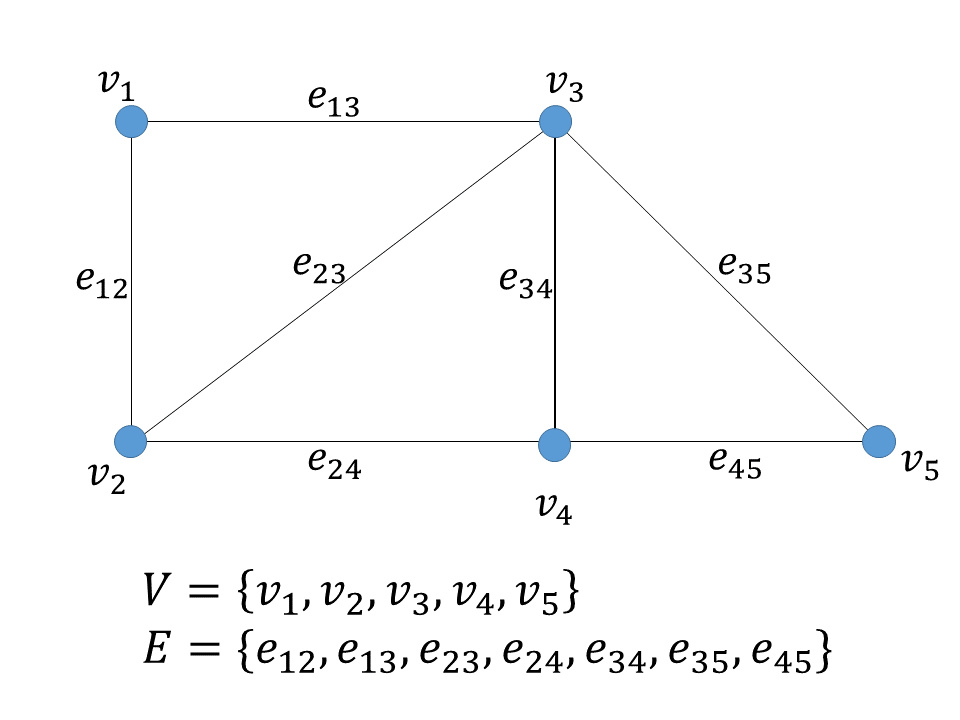
\includegraphics[width = 10cm]{graph1.png}
			\caption{A graph $G = (V, E)$\label{fig:graph}}
		\end{center}
	\end{figure}
	
	A \textbf{complete graph\index{complete graph}} is a simple undirected graph in which every pair of vertices is connected by an edge.
	The complete graph with $n$ vertices is often denoted by $K_n$ (Figure \ref{fig:complete}). 
	It is clear that a complete graph $K_n$ has $n(n-1)/2$ edges.
	
	\begin{figure}[h!]
		\begin{center}
			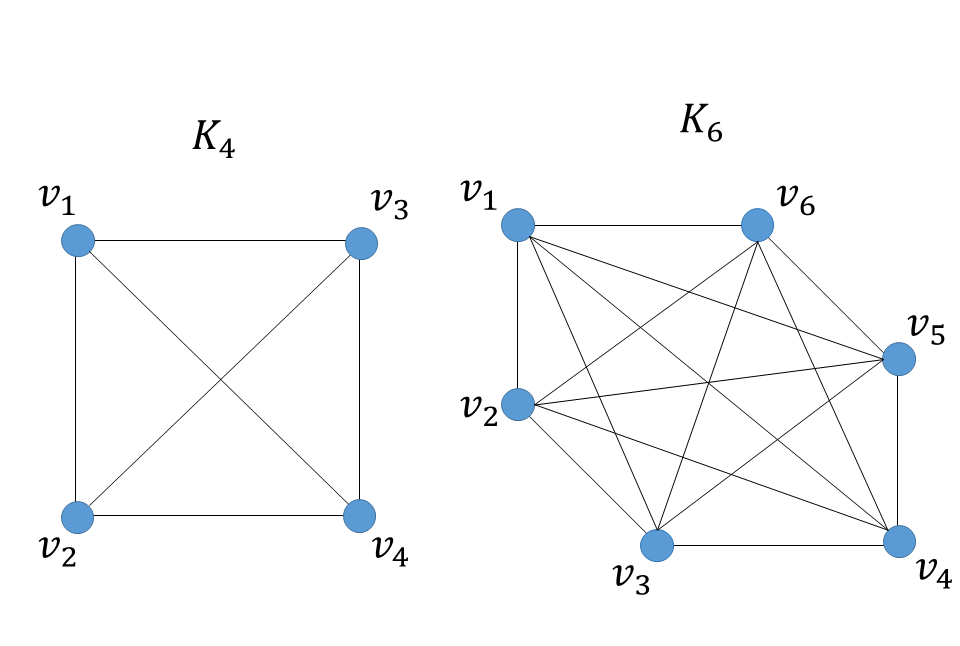
\includegraphics[width = 10cm]{complete.png}
			\caption{Complete graphs\label{fig:complete}}
		\end{center}
	\end{figure}
	
	\section{Paths, Cycles and Connectivity}
	
	For a graph $G = (V, E)$, a \textbf{walk\index{walk}} from $v_i$ to $v_t$ is a finite sequence of edges of the form $e_{ij}, e_{jk}, \ldots , e_{ls}, e_{st}$.
	If the starting vertex and the ending vertex are same, i.e., $v_i = v_t$, we say that the walk is \textbf{closed\index{closed}}.
	The number of edges included in a walk is called its \textbf{length\index{length}}.
	A walk $e_{ij}, e_{jk}, \ldots , e_{ls}, e_{st}$ in which all the edges $\{e_{ij}, e_{jk}, \ldots , e_{ls}, e_{st}\}$ are distinct is called a \textbf{trail\index{trail}}.
	In addition, a walk in which all the vertices $\{v_i, v_j, v_k, \ldots v_l, v_s, v_t\}$ are distinct (except, possibly, $v_i = v_t$) is a \textbf{path\index{path}}.
	A closed path is called a \textbf{cycle\index{cycle}}.
	For vertices $v_i$ and $v_j$, the \textbf{distance} from $v_i$ to $v_j$ is the length of the shortest path from $v_i$ to $v_j$.
	When a graph is directed, there may exist one-way edges in the graph.
	Therefore, in this case the distance from $v_i$ to $v_j$ does not generally coincide with that from $v_j$ to $v_i$.
	\bigskip
	
	We say that a graph is \textbf{connected\index{connected}} if there is a path between each pair of vertices, otherwise it is said to be disconnected (Figure \ref{fig:connected}).
	When a graph is disconnected, it is possible that there is no path between a pair of vertices.
	In this case, we set the distance between them to infinity.
	
	\begin{figure}[h!]
		\begin{center}
			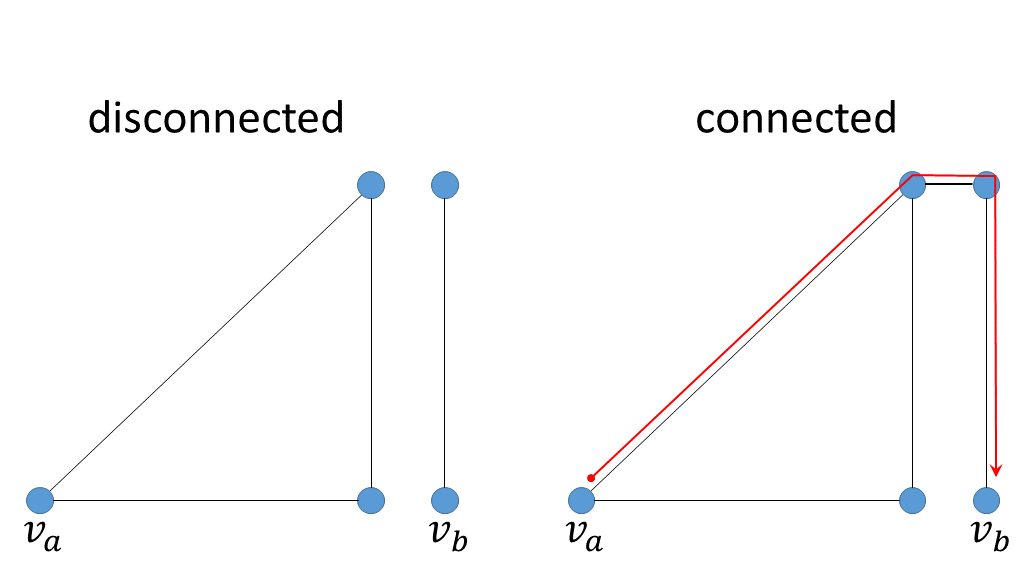
\includegraphics[width = 12cm]{connected.png}
			\caption{Connected/disconnected graph\label{fig:connected}}
		\end{center}
	\end{figure}
	
	The next result provides an easy-to-check sufficient condition for a graph to be connected.
	\begin{proposition}
		Let a graph $G = (V, E)$ be a simple graph with $n \ge 2$ vertices. 
		If the number of edges in $G$ is larger than $(n-1)(n-2)/2$, then the graph is connected.
	\end{proposition}
	
	\begin{proof}
		We prove the result by contradiction.
		Suppose that $G$ is disconnected and is comprised of $k > 1$ connected graph components.
		It is clear that the maximum number of edges that $G$ can contain decreases as $k$ increases.
		Thus, it is sufficient to consider the case $k = 2$.
		Let $G_1$ and $G_2$ be connected graphs with $n_1$ and $n_2$ vertices, respectively, such that $G = G_1 \cup G_2$ ($n_1 + n_2 = n$).
		Here, note that, in order to attain the maximum number of edges, (without loss of generality) $G_1$ must be a single vertex without edges and $G_2$ must be a complete graph $K_{n-1}$.
		Then, since the number of edges in $K_{n-1}$ is equal to $(n-1)(n-2)/2$, the number of edges in $G$ is at most $(n-1)(n-2)/2$, which is a contradiction with the assumption.
		Thus, $G$ is connected.
	\end{proof}
	
	\section{Degree}
	
	For a graph $G = (V, E)$, if there is an edge $e_{ij} \in E$ between $v_i$ and $v_j$, we say that $v_i$ and $v_j$ are \textbf{adjacent\index{adjacent}}.
	In a complete graph, all pairs of vertices are adjacent.
	When $v_i$ and $v_j$ are adjacent, we say that the vertices $v_i$ and  $v_j$ are \textbf{incident\index{incident}} with the edge $e_{ij}$.
	
	\begin{figure}[h!]
		\begin{center}
			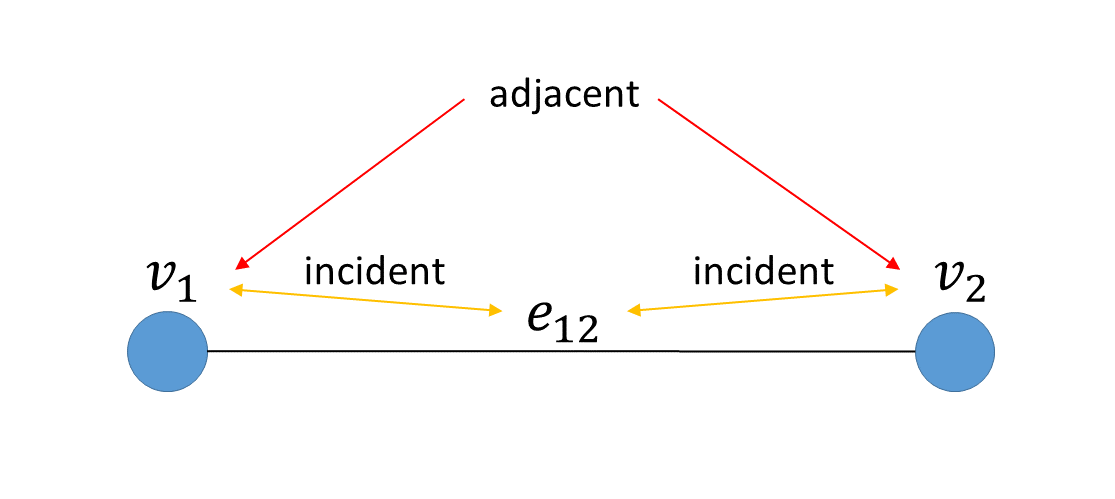
\includegraphics[width = 10cm]{adjacent.png}
			\caption{Adjacency and incidence\label{fig:adjacency}}
		\end{center}
	\end{figure}
	
	The \textbf{degree\index{degree}} of a vertex $v$ of a graph $G$ is the number of edges incident with $v$, which we denote as $d_G(v)$.
	A loop is counted twice in $d_G(v)$.
	A vertex of degree $d_G(v) = 0$ and $d_G(v) = 1$ are said to be \textbf{isolated vertex\index{isolated vertex}} and \textbf{end vertex\index{end vertex}} of $G$, respectively.
	When the graph $G = V(V, E)$ is simple with no loops and multiple edges, the degree of a vertex $v_i \in V$ is equal to the number of vertices adjacent to $v_i$, namely,
	\[
		d_G(v_i) = | \{v_j \in V : e_{ij}\in E\} |,
	\]
	where $| A |$ denotes the cardinality of set $A$.
	For a complete graph $K_n$, the degrees of all vertices are equal to $n - 1$.
	
	\begin{figure}[h!]
		\begin{center}
			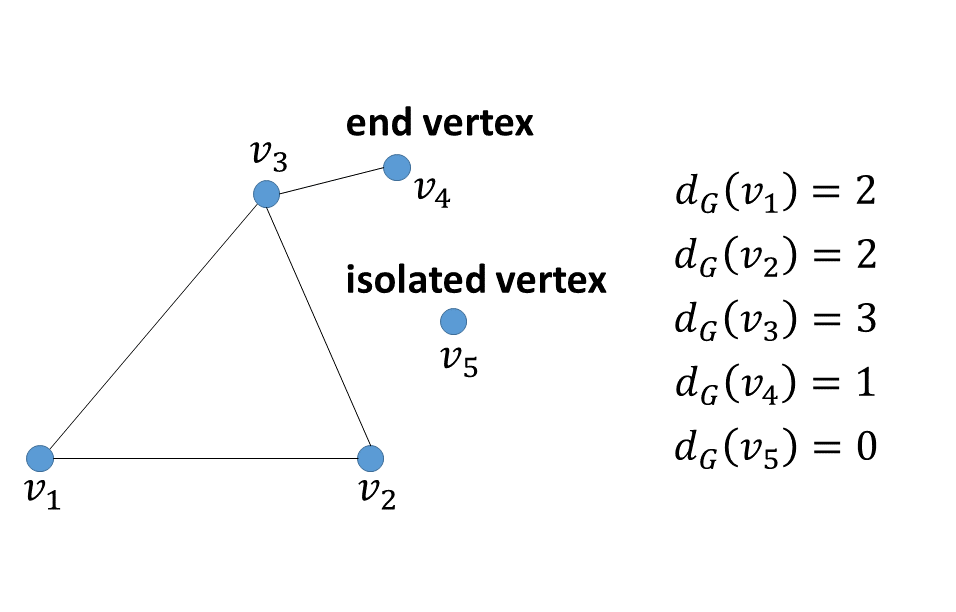
\includegraphics[width = 10cm]{degree.png}
			\caption{Degree\label{fig:degree}}
		\end{center}
	\end{figure}
	
	The next result is often referred to as the ``handshaking'' lemma:
	\begin{proposition}[Handshaking]\label{prop:handshake}
		For any graph $G = (V, E)$, $\sum_{v \in V} d_G(v) = 2 | E |$.
		(The total number of hands shaken is twice the number of handshakes.)
	\end{proposition}
	
	\begin{proof}
		Let $\mathbf{1}(v \sim e)$ be an indicator that takes 1 if $v$ is incident with $e$ and 0 otherwise.
		Then, we can write $d_G(v) = \sum_{e \in E}\mathbf{1}(v \sim e)$.
		Note that each edge contributes 2 to the sum of degrees: $\sum_{v \in V}\mathbf{1}(v \sim e) = 2$ holds for each $e \in E$.
		Thus,
		\begin{align*}
			\sum_{v \in V} d_G(v) 
			& = \sum_{v \in V} \sum_{e \in E}\mathbf{1}(v \sim e) \\
			& = \sum_{e \in E} \;\; \underbrace{\sum_{v \in V} \mathbf{1}(v \sim e)}_{=2} = 2 |E|.
		\end{align*}
	\end{proof}
	
	As a corollary of the above result, we can easily show that the number of vertices of odd degree is even.
	
	\section{Eulerian graph}
	
	A connected graph $G$ is an \textbf{Eulerian graph\index{Eulerian graph}} if there exists a closed trail containing every edge of $G$.
	Such a trail is called an \textbf{Eulerian trail\index{Eulerian trail}}.
	In other words, an Eulerian graph is a graph that can be drawn unicursally without lifting one's pencil from the paper and without repeating any lines.
	
	Then, the problem of K\"onigsberg bridges is equivalent to asking whether the lower-right graph in Figure \ref{fig:euler} has an Eulerian trail.
	In 1736, Euler proved that if the degree of each vertex of $G$ is an even number, then $G$ has an Eulerian trail.
	From this result, we can see that the upper graphs in Figure \ref{fig:euler} are Eulerian, and the lower graphs are not.
	
	\begin{figure}[h!]
		\begin{center}
			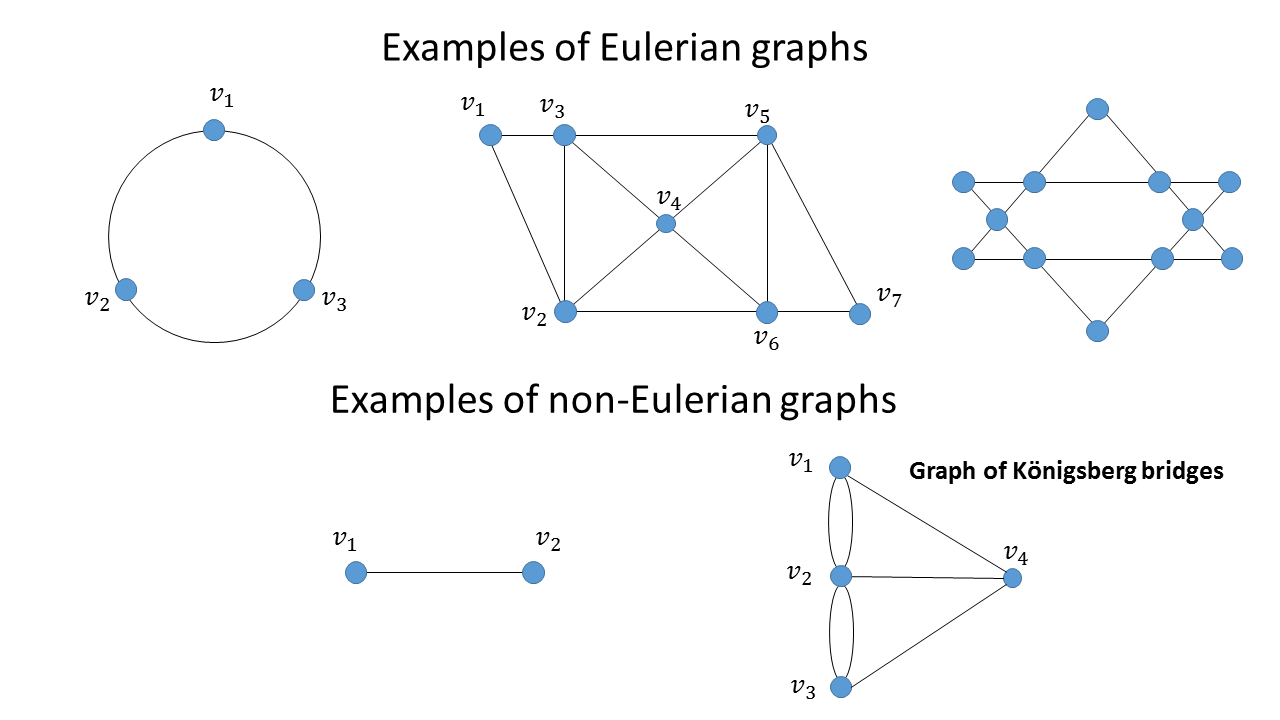
\includegraphics[width = 15cm]{graphs.png}
			\caption{Eulerian graphs and non-Eulerian graphs\label{fig:euler}}
		\end{center}
	\end{figure}
	
	Before providing the proof of this result, we prove the following useful lemma.
	\begin{lemma}\label{lem:cycle}
		If $G$ is a graph in which the degree of each vertex is at least $2$, then $G$ contains a cycle (recall: cycle = closed path).
	\end{lemma}
	
	\begin{proof}
		If $G$ has loops or multiple edges, the result trivially holds.
		Then, suppose that $G$ is a simple graph.
		Let $v$ be any vertex of $G$, and construct a walk starting from $v$, say $v \to v_1 \to v_2 \to \cdots $, by choosing $v_{i+1}$ such that $v_{i+1}$ is adjacent to $v_i$ and $v_{i+1} \neq v_{i-1}$.
		The existence of such walk is guaranteed by the simplicity of $G$ and the assumption made.
		Since the number of vertices if finite, we must eventually choose a vertex that has been chosen before.
		Letting $v_k$ be the first such vertex, the walk contains a cycle starting from $v_k$.
	\end{proof}
	
	Now, we state Euler's (1736) result formally as follows:
	\begin{theorem}
		A connected graph $G = (V,E)$ is Eulerian if and only if the degree of each vertex of $G$ is even.
	\end{theorem}
	
	\begin{proof}
		(Eulerian $\Rightarrow$ the degrees of the vertices are even.) Suppose that $P$ is an Eulerian trail of $G$.
		Whenever $P$ passes through a vertex, there is a contribution of 2 to the degree of that vertex.
		Since each edge appears exactly once in $P$, the degree of each vertex must be even.
		\bigskip
		
		(The degrees of the vertices are even $\Rightarrow$ Eulerian.) We prove the result by induction with respect to $q = |E|$.
		If $q \le 2$, the result trivially holds.
		Then, suppose that $q > 2$ and the result holds for any connected graph $G' = (V', E')$ with $|E'| \le q - 1$.
		Since the degrees of the vertices of $G$ are at least 2, by Lemma \ref{lem:cycle}, we can construct a cycle $C: v_1 \to v_2 \to \cdots \to v_1$ in $G$.
		Let $G_1 = (V_1, E_1)$ be a graph obtained by eliminating the edges in $C$ from $G$.
		Since $|E_1| \le q - 1$, $G_1$ is Eulerian by assumption.
		Here, we can choose a vertex $v^* \in V_1$ which is included in the cycle $C$. 
		Noting that an Eulerian trail can be started at any vertex and it will end at the same vertex, we can construct an Eulerian trail of $G_1$ starting and ending at $v^*$, say $P^*$.
		Then, the cycle $v_1 \to v_2 \to \cdots \to \underbrace{v^* \to \cdots \to v^*}_{P^*} \to \cdots \to v_1$ is an Eulerian trail of $G$.
	\end{proof}
	\section{Adjacency matrix}\label{sec:adjacency}
	
	For a graph $G = (V, E)$ with $n$ vertices $\{v_1, \ldots, v_n\}$, its \textbf{adjacency matrix\index{adjacency matrix}} $A_n = (a_{i,j})$ is the $n \times n$ matrix whose $(i,j)$-th element is the number of edges joining $v_i$ and $v_j$.
	If $G$ has no loops, the diagonal elements of $A_n$ are zero.
	Further, if $G$ has no multiple edges, each $(i,j)$-th element of $A_n$ is an indicator whether $v_i$ is adjacent to $v_j$ or not.
	Adjacency matrix of an undirected graph is symmetric, while that of an directed graph can be asymmetric (Figure \ref{fig:adjmat}).
	The adjacency matrix $A_n$ contains all the information about the graph $G$.
	
	\begin{figure}[h!]
		\begin{center}
			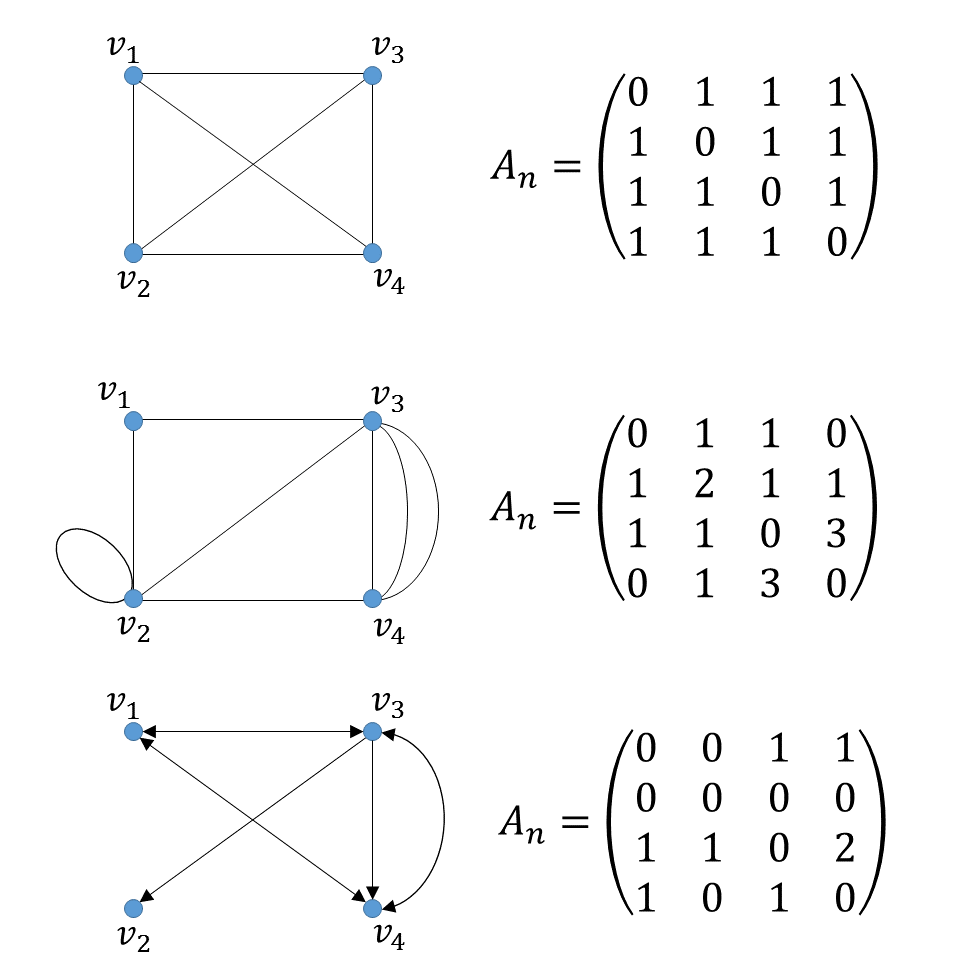
\includegraphics[width = 12cm]{adjmat.png}
			\caption{Adjacency matrix\label{fig:adjmat}}
		\end{center}
	\end{figure}
	
	\subsection*{Some useful properties of adjacency matrix}
	
	\begin{enumerate}
		\item Using the adjacency matrix, the degree of vertex $v_i$ can be calculated as
		\[
			d_G(v_i) = \sum_{j = 1}^n a_{i,j}
		\]
		which is the $i$-th row sum of $A_n$.
		In the case of directed graph, the $i$-th row sum of $A_n$ corresponds to the ``out-degree'' of $v_i$.
		By Proposition \ref{prop:handshake}, it follows that the total number of edges is equal to one-half of the sum of all entries of $A_n$.
		\item For a non-negative integer $\ell$, the $(i,j)$-th element of $A_n^\ell$ equals to the number of walks of length $\ell$ from $v_i$ to $v_j$. (We define $A_n^0$ to be the identity matrix $I_n$.)
		Recall that $a_{ik}$ tells us the number of edges from $v_i$ to $v_k$.
		Hence, the number of walks of length 2 from $v_i$ to $v_j$ passing through $v_k$ is obtained by $a_{ik}a_{kj}$, and the total number of such walks is $\sum_{k = 1}^n a_{ik}a_{kj} = (A_n^2)_{i,j}$.
	
		\begin{figure}[h!]
			\begin{center}
				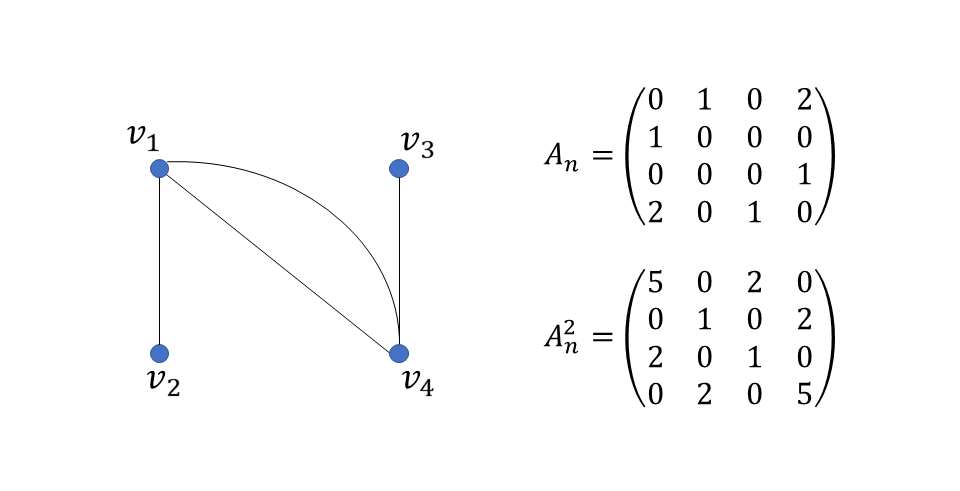
\includegraphics[width = 12cm]{nwalks.png}
				\caption{Number of walks\label{fig:nwalks}}
			\end{center}
		\end{figure}
	
		By using this property, one can easily find the shortest path length between a given pair of vertices.
		For example, suppose that $ (A_n)_{i,j} =  (A_n^2)_{i,j} = \cdots =  (A_n^{\ell - 1})_{i,j} = 0$ and $(A_n^\ell)_{i,j} > 0$. 
		Then, the shortest path length between $v_i$ and $v_j$ is $\ell$.
	\end{enumerate}
	
	\section{Centrality in networks}
	In empirical network analysis, we often want to identify which agents (vertices/nodes) are most ``central''.
	The definition of ``centrality'' varies by contexts and purposes.
	
	The most basic centrality measure is the \textbf{degree centrality\index{degree centrality}} of a vertex $v$, which is simply defined as the degree of $v$, $d_G(v)$.
	The degree centrality is based on an idea that a person who has many connections is the most important person.
	For example, see the graph in Figure \ref{fig:center}.
	For this graph, the most central vertices in terms of the degree centrality are $v_3$ and $v_5$.
	However, in this example, one might consider that $v_4$ is more central than $v_3$ and $v_5$.
	
	Here, let us denote the distance (i.e., the length of the shortest path) between the vertices $v_i$ and $v_j$ by $\Delta(v_i, v_j)$.
	The \textbf{eccentricity\index{eccentricity}} $e(v)$ of a node $v$ in a connected graph $G = (V, E)$ is the maximum distance between $v$ and $u \in V$, that is
	\[
		e(v) = \max_{u \in V} \Delta(v, u).
	\]
	When $G$ is not connected, we define $e(v) = \infty$ for all $v$.
	Then, the reciprocal of the eccentricity value can be also used as a measure of centrality.
	Based on this centrality measure, the most central vertex in the graph in Figure \ref{fig:center} is $v_4$.
	
	More sophisticated centrality measure can be constructed based on the accessibility to other vertices, including not only adjacent vertices but also those that are not adjacent in the graph. 
	Here, recall that the $(i,j)$-th element of the $\ell$-th power of the adjacency matrix $A_n^\ell$ represents the number of walks of length $\ell$ from $v_i$ to $v_j$, where $n$ is the number of vertices in the graph.
	Thus, letting $\mathbf{1}_n$ be the vector of ones of length $n$, the $i$-th element of $A_n^\ell \mathbf{1}_n$ is equal to:
	\[
		(A_n^\ell \mathbf{1}_n)_i = \text{the number of vertices reachable from $v_i$ by length-$\ell$ walk.}
	\]
	Let $\beta \in (0,1)$ be an ``propagation factor'' for an increase of the length.
	(For example, one may interpret $\beta$ as the magnitude of peer effects; or, for another example, the rate of infection of a disease to neighboring residents.)
	Then, we can consider the $i$-th element of $C_n(\beta)$, where
	\[
		C_n(\beta) = \left( \sum_{\ell = 0}^\infty \beta^\ell A_n^\ell \right) \mathbf{1}_n,
	\]
	as the $i$-th centrality value, which is called the \textbf{Bonacich centrality\index{Bonacich centrality}}.
	
	\begin{figure}[h!]
		\begin{center}
			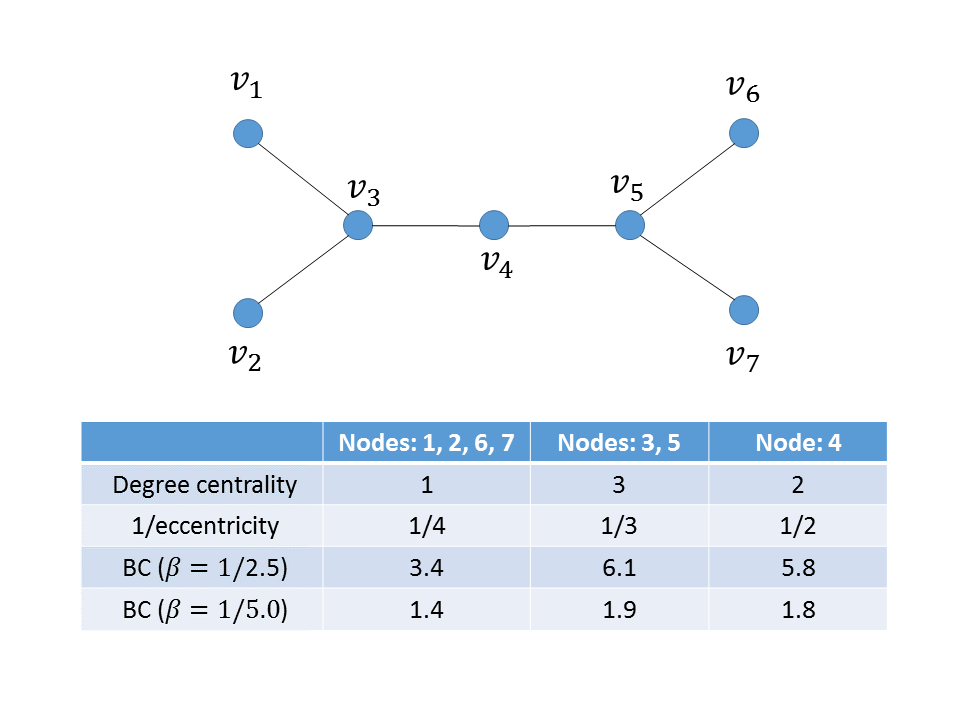
\includegraphics[width = 14cm]{central.png}
			\caption{Centrality measures\label{fig:center}}
		\end{center}
	\end{figure}
	
	In the third and the fourth row of the table in Figure \ref{fig:center}, we report the Bonacich centrality of each vertex with $\beta = 1/2.5$ and $\beta = 1/5$, respectively.
	As we can see, in terms of Bonacich centrality, the centrality of the vertices 3, 4 and 5 becomes more (less) prominent if the propagation factor $\beta$ is large (small).
	
	It is important to note that a higher-order matrix polynomial $\beta^\ell A_n^\ell$ can quickly diverge to infinity for some choice of $\beta$.
	When $\beta$ is appropriately chosen so that $C_n(\beta)$ exists, using the Neumann series formula, it can be exactly obtained by
	\[
	C_n(\beta) = \left(I_n - \beta A_n \right)^{-1}\mathbf{1}_n,
	\]
	where $I_n$ is the $n \times n$ identity matrix (see Appendix \ref{sec:neumann} for details).
	An easy-to-check sufficient condition for the existence of $C_n(\beta)$ is that $\beta \cdot \max_{v \in V}d_G(v) < 1$.
	
	In the literature on network games, the Bonacich centrality has an important role in identifying the \textit{key player}, the player who, once removed from the network, causes the most significant impact on the aggregate outcome such as total welfare of the network (see, e.g., \cite{ballester2006s}).
	
	%%%%%%%%%%%%%%%%%%%%%%%%%%%%%%%%%%%%%%%
	
	\chapter{Supplementary Mathematical Notes}
	\section{Some supplementary results in probability theory.}
	\begin{lemma}\label{lem:prodconv}
	Let $X_n \in \mathbb{R}$ and $Y_n \in \mathbb{R}$ be sequences of random variables such that $X_n \overset{p}{\to} \bar X$ and $Y_n \overset{p}{\to} \bar Y$, respectively, where both $\bar X$ and $\bar Y$ are finite.
	Then, it holds that $X_n Y_n \overset{p}{\to} \bar X \bar Y$.
	\end{lemma}
	
	\begin{proof}
		By the triangle inequality,
		\begin{align*}
		|X_n Y_n - \bar X \bar Y|
		& = |X_n Y_n - \bar X Y_n + \bar X Y_n - \bar X \bar Y| \\
		& \le |X_n Y_n - \bar X Y_n| + |\bar X Y_n - \bar X \bar Y| \\
		& = |Y_n| \cdot |X_n - \bar X| + |\bar X |\cdot | Y_n - \bar Y|. 
		\end{align*}
		The second term on the right-hand side clearly converges to zero in probability.
		For the first term, note that $|Y_n|$ is not necessarily finite for some $n$.
		Let $\kappa > 0$ and $\eta > 0$ be positive numbers.
		 \begin{align*}
		\Pr(|Y_n| \cdot |X_n - \bar X| > \kappa) 
		& = \Pr(|Y_n| \cdot |X_n - \bar X| > \kappa, |Y_n| \le 1/\eta) +	\Pr(|Y_n| \cdot |X_n - \bar X| > \kappa, |Y_n| > 1/\eta) \\
		& \le \Pr(|X_n - \bar X| > \kappa \eta) +	\Pr(|Y_n| > 1/\eta) \\
		& \le \Pr(|X_n - \bar X| > \kappa \eta) +	\Pr(|\bar Y| > 1/(2\eta)) + \Pr(|Y_n - \bar Y| > 1/(2\eta)).
		 \end{align*}
		By choosing sufficiently small $\eta$, the terms on the right-hand side all converge to zero in probability by assumption.
		Thus, we have 
		 \[
		 \lim_{n\to\infty} \Pr(|Y_n| \cdot |X_n - \bar X| > \kappa) = 0.
		 \]
		 Since ths choice of $\kappa$ is arbitrary, this gives the desired result.
	\end{proof}
	
	\begin{lemma}[Slutsky's theorem]\label{lem:slutsky}
		Let $X_n \in \mathbb{R}$ and $Y_n \in \mathbb{R}$ be sequences of random variables such that $X_n \overset{d}{\to} \bar X$ and $Y_n \overset{p}{\to} c$, respectively.
		Then,
		\begin{align*}
		\mathrm{(i)} & \;\; X_n + Y_n \overset{d}{\to} \bar X + c,\\
		\mathrm{(ii)} & \;\; X_n Y_n \overset{d}{\to} c \bar X.
		\end{align*}
		More generally, $g(X_n, Y_n) \overset{d}{\to} g(\bar X, c)$ holds for any continuous function $g(\cdot, \cdot)$. 
	\end{lemma}
	The proof is omitted (see, e.g., Lemma 2.8 in \cite{van2000asymptotic}).
	
	\begin{lemma}[Jensen's inequality]\label{lem:Jensen}
		 Let $X \in \mbb{R}$ be a random variable and $\varphi(\cdot)$ be a convex function.
		 Then,
		\[
			\E[\varphi(X)] \ge \varphi(\E[X]). 
		\]
		If $\varphi(\cdot)$ is concave, then
		\[
			\E[\varphi(X)] \le \varphi(\E[X]). 
		\]
	\end{lemma}
	
	\begin{proof}
		Suppose that $\varphi(\cdot)$ is a convex function.
		Let $L(x) = a + bx$ be a straight line which is tangent to $\varphi(x)$ at $x = \E[X]$.
		Since $\varphi(\cdot)$ is convex, for all $x$, $\varphi(x) \ge L(x)$.
		Thus,
		\begin{align*}
		\E[\varphi(X)] 
		& \ge \E[L(X)] = \E[a + bX] = a + b \E[X] = L(\E[X]) =  \varphi(\E[X]).
		\end{align*}
		\begin{center}
			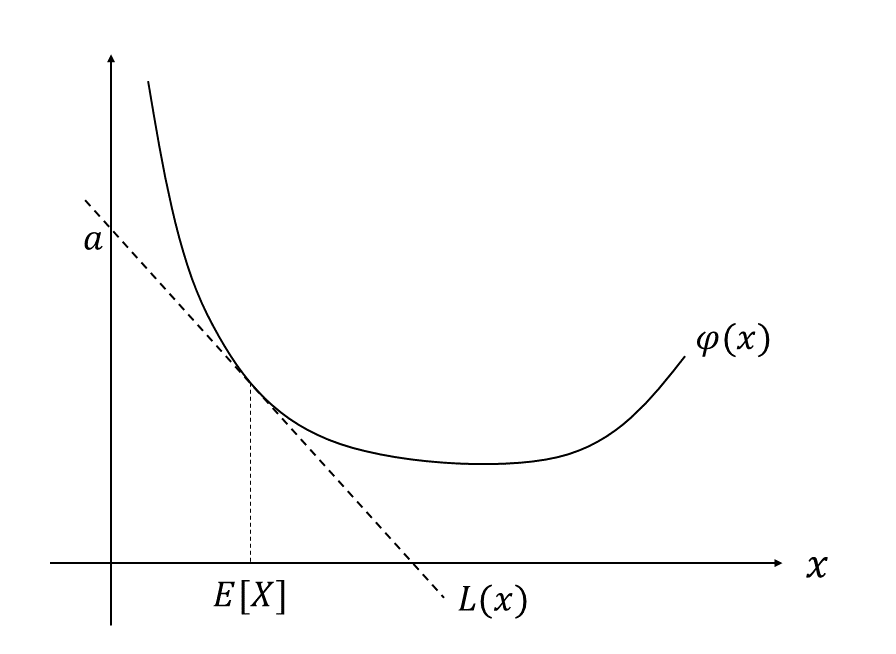
\includegraphics[width = 10cm]{jensen.png}
		\end{center}
	
	\end{proof}
	
	\begin{lemma}[Cauchy-Schwarz inequality]\label{lem:CS}
		For any random variables $X \in \mbb{R}$ and $Y \in \mbb{R}$, we have
		\[
		\left| \E[XY] \right| \le \sqrt{\E[X^2]} \sqrt{\E[Y^2]}. 
		\]
	\end{lemma}
	
	\begin{proof}
		When either $\E[X^2] = 0$ or $\E[Y^2] = 0$ is true, the result follows trivially with equality.
		Thus, we may consider the case where $\E[X^2], \E[Y^2] > 0$.
		Let us define $W = (X - c Y)^2$ for some constant $c$.
		Since $W$ is a non-negative random variable, we must have
		\begin{align*}
			0 
			& \le \E[W] \\
			& = \E[X^2] - 2c\E[XY] + c^2 \E[Y^2].
		\end{align*}
		Further, if we choose $c = \frac{\E[XY]}{\E[Y^2]}$, we have
		\[
			 \E[X^2] - 2c\E[XY] + c^2 \E[Y^2] = \E[X^2] - \frac{\E[XY]^2}{\E[Y^2]}.
		\]
		Combining these results yields the desired result.
	\end{proof}
	%%%%%%%%%%%%%%%%%%%%%%%%%%%%%%%%%%%%%%%
	\section{Neumann series expansion}\label{sec:neumann}
	Let $A = (a_{i,j})$ be a matrix of finite-dimension $n \times m$.\footnote{
		This is just for simplicity.
		In general, we can consider a linear operator $A$ on an infinite dimensional Banach space.
	}
	We use $||A||_\infty$ to denote its infinity-norm: $||A||_\infty \equiv \max_{1 \le i \le n}\sum_{j = 1}^m |a_{i,j}|$.
	
	\begin{lemma}
		The infinity norm is sub-multiplicative.
		That is, for matrices $\underset{n \times m}{A} = (a_{i,j})$ and $\underset{m \times p}{B} = (b_{j,k})$, $||A B ||_\infty \le ||A||_\infty ||B||_\infty$ holds.
	\end{lemma}
	
	\begin{proof}
		\begin{align*}
		||A B ||_\infty
		& = \max_{1 \le i \le n}\sum_{k = 1}^p \left| \sum_{j = 1}^m a_{i,j} b_{j,k} \right| \\
		& \le \max_{1 \le i \le n}\sum_{k = 1}^p \sum_{j = 1}^m | a_{i,j}| \cdot |b_{j,k}| \\
		& =\max_{1 \le i \le n} \sum_{j = 1}^m | a_{i,j}| \sum_{k = 1}^p |b_{j,k}| \\
		& \le \max_{1 \le i \le n} \sum_{j = 1}^m | a_{i,j}| \max_{1 \le j \le m} \sum_{k = 1}^p |b_{j,k}| = ||A ||_\infty ||B||_\infty.
		\end{align*}
	\end{proof}
	
	The series of matrices $\sum_{t = 0}^\infty A^t$ is called the \textbf{Neumann series\index{Neumann series}}.
	The Neumann series has the following important property:
	\begin{lemma}[Neumann series expansion]\label{lem:neumann}
		Suppose that $A_n$ is an $n \times n$ symmetric matrix such that $||A_n||_\infty < 1$.
		Then, $I_n - A_n$ is nonsingular, and it holds that $(I_n - A_n)^{-1} = \sum_{t = 0}^\infty A_n^t$.
	\end{lemma}
	
	\begin{proof}
		The first part is an elementary result in matrix algebra. 
		For the second part, observe that, for some $t$,
		\begin{align*}
		(I_n - A_n) (I_n + A_n + A_n^2 + \cdots + A_n^t) 
		& =  (I_n + A_n + A_n^2 + \cdots + A_n^t)  -  \underbrace{A_n (I_n + A_n + A_n^2 + \cdots + A_n^t) }_{A_n + A_n^2 + \cdots + A_n^{t+1}} \\
		& = I_n - A_n^{t+1}.
		\end{align*}
		Multiplying both sides by $(I_n - A_n)^{-1}$ yields
		\begin{align*}
		& (I_n + A_n + A_n^2 + \cdots + A_n^t)  =   (I_n - A_n)^{-1} - (I_n - A_n)^{-1}A_n^{t+1}, \\
		& \text{and thus } (I_n - A_n)^{-1} - (I_n + A_n + A_n^2 + \cdots + A_n^t) =  (I_n - A_n)^{-1}A_n^{t+1}.
		\end{align*}
		Since the infinity norm is sub-multiplicative, noting that $||A_n||_\infty < 1$ by assumption,
		\begin{align*}
		|| (I_n - A_n)^{-1} - (I_n + A_n + A_n^2 + \cdots + A_n^t)||_\infty 
		& =  ||(I_n - A_n)^{-1}A_n^{t+1}||_\infty \\
		& \le  ||(I_n - A_n)^{-1}||_\infty ||A_n^{t+1}||_\infty \\
		& \le  ||(I_n - A_n)^{-1}||_\infty ||A_n||^{t+1}_\infty \to 0
		\end{align*}
		as $t \to \infty$.
	\end{proof}
	
	\section{Expectation of a truncated random variable}\label{sec:truncate}
	
	Let $X$ be a continuous random variable with its probability distribution function $F(\cdot)$ and density function $f(\cdot)$.
	Further, let $a$ be a constant.
	Then, the conditional distribution of $X$ given that $X \leq a$ is obtained by
	\begin{align*}
	F(x \mid X \leq a)
	& = \Pr(X \leq x \mid X \leq a)\\
	& = \frac{\Pr(X \leq \min\{x, a\})}{\Pr(X \leq a)} = \left\{\begin{array}{cl}
	1 & \text{ if $x \geq a$} \\ 
	\frac{F(x)}{F(a)} & \text{ if $x < a$}
	\end{array}	\right. .
	\end{align*}
	By differentiating the both sides with respect to $x$, the conditional density of $X$ given that $X \leq a$ is given by
	\begin{align*}
	f(x \mid X \leq a) = \left\{\begin{array}{cl}
	0 & \text{ if $x \geq a$} \\ 
	\frac{f(x)}{F(a)} & \text{ if $x < a$}
	\end{array}	\right. .
	\end{align*}
	Thus, the expectation of $X$ conditional on $X \leq a$ is
	\begin{align*}
	\E[X \mid X \leq a] 
	& = \int_{-\infty}^{\infty} x f(x \mid X \leq a) \mrm{d}x \\
	& = \frac{\int_{-\infty}^a x f(x) \mrm{d}x}{F(a)}.
	\end{align*}
	By analogous arguments, we can show that the expectation of $X$ conditional on $X > a$ is obtained by
	\begin{align*}
	\E[X \mid X > a] 
	& = \int_{-\infty}^{\infty} x f(x \mid X > a) \mrm{d}x \\
	& = \frac{\int_a^\infty x f(x) \mrm{d}x}{1 - F(a)}.
	\end{align*}
	
	\section{The inverse of a partitioned matrix}
	Consider a partitioned matrix
	\[
		A = \left(\begin{array}{cc}
		A_{11} & A_{12} \\
		A_{21} & A_{22}
	\end{array}	\right).
	\]
	Then, the inverse of $A$ is given by
	\begin{align}\label{eq:inverse}
		A^{-1} = \left(\begin{array}{cc}
		(A_{11} - A_{12}A_{22}^{-1}A_{21})^{-1} & -(A_{11} - A_{12}A_{22}^{-1}A_{21})^{-1}A_{12}A_{22}^{-1} \\
		-(A_{22} - A_{21}A_{11}^{-1}A_{12})^{-1}A_{21}A_{11}^{-1} & (A_{22} - A_{21}A_{11}^{-1}A_{12})^{-1}
	\end{array} \right).
	\end{align}
	\end{appendices}
	

\clearpage	
\bibliography{references}

\printindex

\end{document}